%; whizzy -pdf .
\documentclass[10pt]{book}
\usepackage{url,hyperref,clrscode,amsmath,amsthm,apalike,fancyhdr,booktabs}
\usepackage[sf,bf,tiny]{titlesec} %add bf for boldface titles
\usepackage{pgf,tikz,pgflibraryshapes,pgflibraryarrows,pgfbaselayers,pgfbaseplot}
\usepackage{multirow,colortbl}
\usepackage[paperwidth=5.82in,paperheight=7.76in,marginparwidth=.75in,marginparsep=.3in,left=.25in,right=.25in,top=.1in,bottom=.1in]{geometry}
%\usepackage[marginparwidth=1.5in,marginparsep=.2in,left=.75in,right=2in,top=.75in,bottom=.75in,paperwidth=6in,paperheight=9in]{geometry}
\usepackage[small,labelfont={sf,bf}]{caption}

%\usepackage[margincaption,ragged]{sidecap} 
\newenvironment{SCfigure}{\begin{figure}}{\end{figure}}
\newenvironment{SCtable}{\begin{table}}{\end{table}}

\usepackage{mparhack}%fixes a bug where margin notes sometimes appeared on wrong side

%Add two special symbols: a filled circle and an open circle
\usepackage{wasysym}
\newcommand{\medbullet}{\mbox{\wasyfamily\char32}}
\newcommand{\medcirc}{\mbox{\wasyfamily\char35}}

\newcounter{exercise}
\newenvironment{exercises}{\section*{Exercises}\addcontentsline{toc}{section}{Exercises}\begin{list}
{\arabic{chapter}.\arabic{exercise}}
{\usecounter{exercise}}}{\end{list}}

%\usepackage[urw-garamond]{mathdesign} %does not have boldface for rm font.

%\usepackage{eco} %use oldstyle (lowercase) numbers. Unf. the numbers
%are type 3 so we'll need to use something else.

%\usepackage{adobegaramond} %font bought from Adobe, seems to work well
%with CM math but does not have sans-serif font.

%Use times fonts
%\usepackage{mathptmx}

%Set up times roman as the main font and adobe helvetica (95%) as the
%sans serif fong. Adds support  for some special characters, like the circles.
%\usepackage{txfonts} 

%Intro to game theory uses mathpazo 10pt, Palatino font
%\usepackage{mathpazo} 
%check out mathdesign package for more fonts

\usepackage{makeidx}
\makeindex


%headers
\pagestyle{fancy}
\fancyhead{} % clear all header fields
%\fancyhead[RO]{\textsf{\rightmark}}
%\fancyhead[LE]{\textsf{\leftmark}}
\fancyhead[RO]{\nouppercase{\textsf{\textbf{\rightmark}}}\hfill\textbf{\thepage}}
\fancyhead[LE]{\textbf{\thepage}\hfill\nouppercase{\textsf{\textbf{\leftmark}}}}

%\fancyheadoffset[RO,LE]{\marginparwidth+\marginparsep}

%\fancyhead[LE]{\slshape \leftmark}
%\fancyfoot[C]{\thepage}
\fancyfoot{}
\renewcommand{\headrulewidth}{0.4pt}
\renewcommand{\footrulewidth}{0pt}
\setlength{\headheight}{15pt} 

%Don't leave blank spaces
\renewcommand{\topfraction}{.9}
\renewcommand{\bottomfraction}{.7}
\renewcommand{\textfraction}{.1}
\renewcommand{\floatpagefraction}{.9}

%hyphenated words
\hyphenation{re-in-force-ment a-syn-chro-nous com-bi-na-to-rial}


%Make empty pages trully empty
\makeatletter
\def\cleardoublepage{\clearpage\if@twoside \ifodd\c@page\else
  \hbox{}
  \vspace*{\fill}
  \begin{center}
%    This page intentionally left blank.
  \end{center}
  \vspace{\fill}
  \thispagestyle{empty}
  \newpage
  \if@twocolumn\hbox{}\newpage\fi\fi\fi}
\makeatother

%marginal comments. Changing the c to a t moves the box down.
\newcommand{\mc}[1]{\marginpar{\mbox{}\fbox{\raggedright
        \begin{minipage}[c]{\marginparwidth}\raggedright
          {\small #1}
        \end{minipage}}}}

%term definition
%\newcommand{\td[1]{\mbox{}\textbf{#1}\marginpar{\center
%\textsc{#1}}}

%place the terms flush against the outside
\usepackage{chngpage}
\newcommand{\td}[1]{\mbox{}\textbf{#1}\index{#1}\marginpar{%
\checkoddpage\ifcpoddpage\raggedleft\else\raggedright\fi\textsc{#1}}}
%\tdi{name as it looks}{name to be indexed}
\newcommand{\tdi}[2]{\mbox{}\textbf{#1}\index{#2@#1}\marginpar{%
\checkoddpage\ifcpoddpage\raggedleft\else\raggedright\fi\textsc{#1}}}
\newcommand{\idx}[1]{#1\index{#1}}
\newcommand{\idxi}[2]{#1\index{#2@#1}}


%netlogo links...could use cooltooltips package from CTAN for pop-up messages.
\newcommand{\netlogo}[1]{\marginpar{%
\begin{center}
\tikz[x=.5cm,y=.5cm,line width=1pt]{\draw (0,0) -- (1,2) -- (2,0) --
  (1,.5) -- cycle;}

\texttt{\href{http://jmvidal.cse.sc.edu/netlogomas/#1.html}{#1}}
\end{center}}}

%hypersetup for pdf
\hypersetup{ %bookmarksopen,
  bookmarksnumbered,   
  colorlinks=false,
  pdfborder=0 0 0, %eliminate hyperlink highlighting
  pdftitle={Fundamentals of Multiagent Systems},
  pdfauthor={Jose M. Vidal},
  pdfsubject={},
  pdfkeywords={multiagent systems, game theory, economics},
  %FitBH=fit visible, FitH=fit width.
  pdfview=FitH,
  pdfstartview=FitH
}

%probabilities
\newcommand{\Pro}{\ensuremath{\mathbf{Pr}}}
%vectors
\newcommand{\vu}{\ensuremath{\vec{u}}} %outcome
\newcommand{\vv}{\ensuremath{\vec{v}}} %another outcome
\newcommand{\va}{\ensuremath{\vec{a}}} %actions
\newcommand{\vA}{\ensuremath{\vec{A}}} %actions
\newcommand{\vb}{\ensuremath{\vec{b}}} %beliefs in POMDP
\newcommand{\bidi}{\ensuremath{b^{\text{items}}}}
\newcommand{\bidp}{\ensuremath{b_1}}
\newcommand{\bidpi}{\ensuremath{b_1^{\text{items}}}}
\newcommand{\bidv}{\ensuremath{b^{\text{value}}}}
\newcommand{\bidpv}{\ensuremath{b_1^{\text{value}}}}
\newcommand{\bida}{\ensuremath{b^{\text{agent}}}}
\newcommand{\astar}{\ensuremath{A^*}}
\newcommand{\idastar}{\ensuremath{IDA^*}}
%acronyms
\newcommand{\acro}[1]{\textsc{#1}}

%pgf stuff
%a stick-figure person
\newcommand{\person}[1]{%
\draw #1 circle (.1cm)
++(0,-.1) -- ++(0,-.4) -- ++(-.2, -.3) 
++(.4,0) -- ++(-.2,.3) 
++(0,.2) -- ++(-.3,-.1)
++(.3,.1) -- ++(.3,-.1);}
%default style for all tikzpictures
\tikzstyle dstyle=[line width=1pt]
\tikzstyle thinline=[line width=.1pt]


\newcommand{\hreffoot}[2]{\href{#1}{#2}}

%theorems
\newtheorem{theorem}{Theorem}[chapter]
\newtheorem{assumption}{Assumption}[chapter]
\newtheorem{definition}{Definition}[chapter]


%snugbox came from usenet, via google. I use it when placing text
%inside pgf nodes.
\makeatletter
\def\snugbox{\hbox\bgroup\setbox\z@\vbox\bgroup
    \leftskip\z@\expandafter\let\expandafter\\\csname @normalcr\endcsname
    \bgroup\aftergroup\make@snug\noindent
    \let\next=}
\def\make@snug{\par\sn@gify\egroup \box\z@\egroup}
\def\sn@gify
   {\skip\z@=\lastskip \unskip
    \advance\skip\z@\lastskip \unskip
    \unpenalty
    \setbox\z@\lastbox
    \ifvoid\z@ \nointerlineskip \else {\sn@gify} \fi
    \hbox{\unhbox\z@}\nointerlineskip
    \vskip\skip\z@
    }
\makeatother

%pictures of famous people on the margins
%\mp{picture filename}{name of person}{birth}{death}{other}
\newcommand{\mpic}[5]{\mc{\includegraphics[width=\marginparwidth]{#1}
    #2. \oldstylenums{#3}--\oldstylenums{#4}. #5}}
\newcommand{\mpicnd}[3]{\mc{\includegraphics[width=\marginparwidth]{#1}
    #2. #3}}

%Elements of Typographical style tips:
%Get rid of extra space after period.
\frenchspacing
\begin{document}

\thispagestyle{empty} %cover page
\phantom{a} %ugly hack, but otherwise vspace does not work
\vspace{3in}
{\Large Fundamentals \emph{of}}

\smallskip

{\Huge Multiagent Systems}

\smallskip

with NetLogo Examples

\bigskip

\hspace{1in}{\Large \emph{Jos\'{e} M Vidal}}

\vspace{1in}


\hfill\textsc{\today}


\newpage %copyright page
\phantom{a} 
\vspace{3in}
\thispagestyle{empty}
\textbf{Fundamentals of Multiagent Systems}

by Jos\'{e} M. Vidal

\smallskip

Copyright \textcopyright{} 2007 Jos\'{e} M. Vidal. All rights reserved.

\tableofcontents
% Add a BDI architecture chapter? 

%Thanks to
%Jiangbo Dang, Huang Jingshan

\chapter*{Preface}
\addcontentsline{toc}{chapter}{Preface}

The goal of this book is to cover all the material that a competent
multiagent practitioner or researcher should be familiar with. Of
course, since this is a relatively new field the list of required
material is still growing and there is some uncertainty as to what are
the most important ideas. I have chosen to concentrate on the
theoretical aspects of multiagent systems since these ideas have been
around for a long time and are important for a wide variety of
applications. I have stayed away from technological issues because
these are evolving very fast.  Also, it would require another textbook
to describe all the distributed programming tools available. A reader
interested in the latest multiagent technologies should visit the
website \url{www.multiagent.com}.

The book is linked to a large number of sample NetLogo programs
\cite{netlogo}.  These programs are meant to be used by the reader as
an aid in understanding emergent decentralized behaviors. It is hard
for people, especially those new to distributed systems, to fully
grasp the order that can arise from seemingly chaotic simple
interactions. As Resnick notices:\mc{Resnick points to examples such
  as surveys of 8--15 year old kids, half of which believe that the
  government sets all prices and salaries.}
\begin{quotation}
  \emph{``But even as the influence of decentralized ideas grows, there is a
  deep-seated resistance to such ideas. At some deep level, people
  seem to have strong attachments to centralized ways of
  thinking. When people see patterns in the world (like a flock of
  birds), they often assume that there is some type of centralized
  control (a leader of the flock). According to this way of thinking,
  a pattern can exist only if someone (or something) creates and
  orchestrates the pattern. Everything must have a single cause, and
  ultimate controlling factor. The continuing resistance to
  evolutionary theories is an example: many people still insist that
  someone or something must have explicitly designed the complex,
  orderly structures that we call Life.''} \cite{resnick94a}
\end{quotation}\mc{Resnick created StarLogo in order to teach the
  \emph{decentralized} mindset. Wilensky, one of his students, later
  extended StarLogo and created NetLogo.}


The reader is assumed to be familiar with basic Artificial
Intelligence techniques \cite{russell03a}. The reader should also be
comfortable with mathematical notation and basic computer science
algorithms. The book is written for a graduate or advanced
undergraduate audience. I also recommend
\cite{mas-colell95a,osborne99a} as reference books.


\section{Usage}
\label{sec:usage}

If you are using the \textsc{pdf} version of this document you can
click on any of the citations and your \textsc{pdf} reader will take
you to the appropriate place in the bibliography. From there you can
click on the title of the paper and your web browser will take you to
a page with a full description of the paper. You can also get the full
paper if you have the user-name and password I provide in class. The
password is only available to my students due to licensing
restrictions on some of the papers.

Whenever you see an icon such as the one on this margin
\netlogo{ABTgc} it means that we have NetLogo implementation of a
relevant problem. If you are using the \textsc{pdf} version of this
document you can just click on the name and your browser will take you
to the appropriate applet. Otherwise, the \textsc{url} is formed by
pre-pending \url{http://jmvidal.cse.sc.edu/netlogomas/} to the name
and appending \url{.html} at the end. So the \textsc{url} for this
icon is \url{http://jmvidal.cse.sc.edu/netlogomas/ABTgc.html}.


\section{Acknowledgments}

I would like to thank the students at the University of South Carolina
who have provided much needed feedback on all revisions of this book.
Specifically, I thank Jimmy Cleveland, Jiangbo Dang, Huang Jingshan,
and Alicia Ruvinsky. I am also especially grateful to faculty members
from other Universities who have used this book in their classes and
provided me with invaluable feedback. Specifically I thank Ram\'{o}n
F. Brena, Muaz Niazi, and Iyad Rahwan.



%%% Local Variables: 
%%% mode: latex
%%% TeX-master: "~/wp/mas/mas"
%%% TeX-command-default: "PDFlatex"
%%% End:



\chapter{Multiagent Problem Formulation}
\label{cha:problemfor}


The goal of multiagent systems' research is to find methods that allow
us to build complex systems composed of autonomous agents who, while
operating on local knowledge and possessing only limited abilities,
are nonetheless capable of enacting the desired global behaviors. We
want to know how to take a description of what a \emph{system of
  agents} should do and break it down into individual agent behaviors.
At its most ambitious, multiagent systems aims at reverse-engineering
emergent phenomena as typified by ant colonies, the economy, and the
immune system. Multiagent systems approaches the problem using the
well proven tools from game theory, Economics, and Biology. It
supplements these with ideas and algorithms from artificial
intelligence research, namely planning, reasoning methods, search
methods, and machine learning.

\mc{A more relaxed introduction to the topics in this chapter is given
  in \cite[Chapters 16--17]{russell03a}.} These disparate influences
have lead to the development of many different approaches, some of
which end up being incompatible with each other.  That is, it is
sometimes not clear if two researchers are studying variations of the
same problem or completely different problems.  Still, the model that
has thus far gained most attention, probably due to its flexibility as
well as its well established roots in game theory and artificial
intelligence, is that of modeling agents as utility maximizers who
inhabit some kind of Markov decision process.  This is the model we
present in this chapter and the one we will use most often throughout
the book. Note, however, that while this is a very general model it is
not always the best way to describe the problem.  We will also examine
the traditional artificial intelligence planning model and, in later
chapters, models inspired by Biology. Another popular model is that of
agents as logical inference machines. This model is favored by those
working on semantic or logical applications. We will sometimes make
reference to \td{deductive} agents which can deduce facts based on the
rules of logic, and \td{inductive} agents (see
Chapter~\ref{cha:learn-mult-syst}) which use machine learning
techniques to extrapolate conclusions from the given evidence.


\section{Utility}

A common simplifying assumption is that an agent's preferences are
captured by a \td{utility function}.  This function provides a map
from the states of the world or outcome of game to a real number.
\mc{In game theory it is known as the von Neumann-Morgenstern utility
  function.} The bigger the number the more the agent likes that
particular state.  Specifically, given that $S$ is the set of states
in the world the agent can perceive then agent $i$'s utility function
is of the form

\begin{equation}
  \label{eq:utility}
  u_i : S \rightarrow \Re.
\end{equation}

Notice also that the states are defined as those states of the world
that the agent can perceive. For example, if a robot has only one
sensor that feeds him a binary input, say 1 if it is bright and 0 if
its dark, then that robot has a utility function defined over only two
states regardless of how complicated the real world might be, such as
$u_i(0) = 5$, $u_i(1) = 10$. In practice, agents have sophisticated
inputs and it is impractical to define a different output for each
input. Thus, most agents also end up mapping their raw inputs to a
smaller set of world states. Creating this mapping function can be
challenging as it requires a deep understanding of the problem
setting.

Given an agent's utility function we can define a \td{preference
  ordering} for the agent over the states of the world.  By comparing
the utility values of two states we can determine which one is
preferred by the agent. This ordering has the following properties.
\begin{itemize}
\item \emph{reflexive}: $u_i(s) \geq u_i(s)$
  
\item \emph{transitive}: If $u_i(a) \geq u_i(b)$ and $u_i(b) \geq u_i(c)$ then $u_i(a) \geq u_i(c)$.
  
\item \emph{comparable}: $\forall_{a,b}$
  either $u_i(a) \geq u_i(b)$ or $u_i(b) \geq u_i(a)$. 
\end{itemize} 

We can use utility functions to describe the behavior of almost every
agent. Utility functions are also useful for capturing the various
tradeoffs that an agent must make, along with the value or expected
value of its actions. For example, we can say that a robot receives a
certain payment for delivering a package but also incurs a cost in
terms of the electricity used as well as the opportunity cost---he
could have been delivering other packages. If we translate all these
payments and costs into utility numbers then we can easily study the
tradeoffs among them.

Once we have defined a utility function for all the agents then all
they have to do is take actions which maximize their utility. As in
game theory, we use the word \td{selfish} to refer to a rational agent
that wants to maximize its utility. Notice that this use is slightly
different from the everyday usage of the word which often implies a
desire to harm others, a true selfish agent cares exclusively about
its utility. The use of selfish agents does not preclude the
implementation of cooperative multiagent systems.
\mc{\textbf{selfish}, adj.  Devoid of consideration for the
  selfishness of others. ---\emph{The Devil's Dictionary}}We can view
a cooperative multiagent system as one where the agents' utility
functions have been defined in such a way so that the agents seem to
cooperate. For example, if an agent receives a higher utility for
helping other agents then the resulting behavior will seem cooperative
to an observer even though the agent is acting selfishly.

We use utility functions as a succinct way of representing an agent's
behavior. In the actual implementations these functions will sometimes
be probabilistic, sometimes they will be learned as the agent acts in
the world, sometimes they will be incomplete, sometimes they will be
the result of some inferencing or induction. Still, by assuming that
the function exists we can more easily design and study a multiagent
system.


\subsection{Utility is Not Money}
\label{sec:money}

Note that while utility represents an agent's preferences it is not
necessarily equated with money. In fact, the utility of money has been
found to be roughly logarithmic. For example, say Bill has \$100
million while Tim has \$0 in the bank. They both contemplate the
possibility of winning one million dollars. Clearly, that extra
million will make a significant difference in Tim's lifestyle while
Bill's lifestyle will remain largely unchanged, thus Tim's utility for
the same million dollars is much larger than Bill's. There is
experimental evidence that shows most people have these type of
conditional preferences. Very roughly, people's utility for smaller
amounts of money is linear but for larger amounts it becomes
logarithmic. Notice that we are considering the \td{marginal utility}
of money, that is, it is the utility for the next million dollars.  We
assume that both Bill and Tim have the same utility for their first
million dollars.  \mc{You can determine your own curve by repeatedly
  asking yourself for increasing values of $x$: which one would you
  rather have, $x$ dollars, or a $50/50$ chance at winning $2\cdot x$
  dollars? When you start preferring the first choice you are dropping
  below the $y=x$ line.}

Recent results in behavioral economics have shown that the true
utility function is more complicated than what can be captured by a
mathematical function \cite{camerer03a}. One experiment shows that
people are less likely to take a gamble when the wording of the
question is such that the person must give back some money, even if
the gamble is mathematically identical to another one that uses
different wording. The experiment in question is the following: which
option would you prefer (a) I give you \$10,000 and a 50/50 chance at
winning another \$10,000, or (b) I give you \$20,000 and then flip a
coin and if it comes out heads you have to give me \$10,000. Both of
these are equivalent but a large majority of people prefer option (a).

The fact that people are not entirely rational when making choices
about money becomes important to us when we start to think about
building agents that will buy, sell, or negotiate for humans. It is
reasonable to assume that in these systems people will demand agents
that behave like people. Otherwise, the agent would be making
decisions the user finds disagreeable. People's apparent irrationality
also opens up the possibility that we could build agents that are
better negotiators than us.

\subsection{Expected Utility}
\label{sec:expected-utility}

Once we have utility functions we must then determine how the agents
will use them. We assume each agent has some sensors which it can use
to determine the state of the world and some effectors which it can
use to take action.  These actions can lead to new states of the
world. For example, an agent senses its location and decides to move
forward one foot. Of course, these sensors and effectors might not
operate perfectly: the agent might not move exactly one foot or its
sensors might be noisy. Let's assume, however, that the agent does
know the probability of reaching state $s'$ given that it is in state
$s$ and takes action $a$. This probability is given by $T(s,a,s')$
which we call the \td{transition function}. Since the transition
function returns a probability then it must be true that the sum of
$T(s,a,s')$ over all possible $a$ and $s'$ is equal to one.

Using this transition function the agent can then calculate its
\td{expected utility} for taking action $a$ in state $s$ as
\begin{equation}
  \label{eq:mod-eu}
  E[u_i,s,a] = \sum_{s' \in S} T(s,a,s')u_i(s'),
\end{equation}
where $S$ is the set of all possible states. 

An agent can use the expected utility function to determine the value
of a piece of added information it might acquire such as an extra
sensor reading or a message from another agent. For example, consider
a piece of new information that leads the agent to determine that it
is not really in state $s$ but it is instead in state $t$. Perhaps a
second agent tells him that he is near a precipice and not in the
middle of a plateau as the agent originally thought. In this case the
agent can compare the expected utility it would have received under
the old state against the new one it will now receive. That is, the
\td{value of information} for that piece of information is given by
\begin{equation}
  \label{eq:mod-valueinfo}
  E[u_i,t,\pi_i(t)] -  E[u_i,t,\pi_i(s)].
\end{equation}
The value of the piece of information is the expected utility the
agent receives now that he knows he is in $t$ and takes action
accordingly minus the utility it would have received if he had instead
mistakenly assumed it was in $s$ and taken action accordingly. This
equation provides a simple and robust way for agents to make
meta-level decisions about what knowledge to seek: what messages to
send, which sensors to turn on, how much deliberation to perform, etc.

Specifically, an agent can use it to play \emph{``what if''} games to
determine its best action in the same way a person might. For example,
say a doctor has made a preliminary decision about which drug to
prescribe for a patient but is uncertain about the patient's specific
disease. She can calculate the value of information acquired from
performing various tests which could identify the specific disease. If
a test, regardless of its outcome, would still lead the doctor to
prescribe the same drug then the value of the information from that
test's result is zero: it does not lead to a change in action so
\eqref{eq:mod-valueinfo} is zero. On the other hand, a test that is
likely to change the doctor's action will likely have a high value of
information.


\section{Markov Decision Processes}
\label{sec:mark-decis-proc}
\mpic{models/markov2}{Andrey Markov}{1856}{1922}{}


So far we have assumed that only the agent can change the state of the
world. But, the reality in most cases is that agents inhabit an
environment whose state changes either because of the agent's action
or due to some external event. We can think of the agent sensing the
state of the world then taking an action which leads it to a new
state. We also make the further simplifying assumption that the choice
of the new state therefore depends only on the agent's current state
and the agent's action. This idea is formally captured by a \td{Markov
  decision process} or \acro{mdp}.
\begin{definition}[Markov Decision Processess]
  An \acro{mdp} consists of an initial state $s_1$ taken from a set of
  states $S$, a transition function $T(s,a,s')$ and a reward function
  $r: S \rightarrow \Re$.
\end{definition}

The transition function $T(s,a,s')$ gives us the probability that an
agent in state $s$ who takes action $a$ will end up in state $s'$.
For a purely \td{deterministic} world we have that this function will
be zero for all $s'$ of each given $s,a$ pair except one, for which it
will be one.  That is, in a deterministic world an agent's action has
a completely predictable effect. This is not the case for a
\td{non-deterministic} environment where an agent's action could lead
to a number of different states, depending on the value of this fixed
probability function.

\begin{SCfigure}
  \begin{minipage}{1.0\linewidth}
    \begin{center}
      \begin{tikzpicture}
        \node[draw,circle] (s1) at (0,0) {$s_1$};
        \node[draw,circle] (s2) at (0,3) {$s_2$};
        \node[draw,circle] (s3) at (3,3) {$s_3$};
        \node[draw,circle] (s4) at (3,0) {$s_4$};
        \draw[->] (s1) .. controls (-.3,1.5)
        .. node[above,sloped] {$a_1: 0.8$} (s2);
        \draw[->] (s1) .. controls (-1,-1) and (-1,0) .. node[left]
        {\snugbox{$a_1 : 0.2$ \\$a_2 : 0.2$}} (s1);
        \draw[->] (s1) .. controls (1.5,.3) .. node[above,sloped]
        {$a_2 : 0.8$} (s4);
        \draw[->] (s2) .. controls (.3,1.5) .. node[above,sloped]
        {$a_3 : 0.8$} (s1);
        \draw[->] (s2) .. controls (1.5,3.3) .. node[above,sloped]
        {$a_2 : 0.8$} (s3);
        \draw[->] (s2) .. controls (-1,3) and (-1,4) .. node[left]
        {\snugbox{$a_2 : 0.2$ \\ $a_3 : 0.2$}} (s2);
        \draw[->] (s3) .. controls (1.5,2.7) .. node[below,sloped]
        {$a_4 : 1$} (s2);
        \draw[->] (s3) .. controls (3.3,1.5) .. node[above,sloped]
        {$a_3 : 1$} (s4);
        \draw[->] (s4) .. controls (2.7,1.5) ..
        node[above,sloped] {$a_1 : 0.9$} (s3);
       \draw[->] (s4) .. controls (4,-1) and (4,0) .. node[right]
       {\snugbox{$a_1 : 0.1$\\$a_4 : 0.2$}} (s4);
       \draw[->] (s4) .. controls (1.5,-.3) .. node[below,sloped]
       {$a_4: 0.8$} (s1);

        \node[below] (t) at (7.8,6.5)  {
          \begin{tabular}{cccr} \toprule
            $s_i$ & $a$ & $s_j$ & $T(s_i,a,s_j)$ \\ \midrule
            $s_1$ & $a_1$ & $s_1$ & $0.2$ \\
            $s_1$ & $a_1$ & $s_2$ & $0.8$ \\
            $s_1$ & $a_2$ & $s_1$ & $0.2$ \\
            $s_1$ & $a_2$ & $s_4$ & $0.8$ \\ 
            $s_2$ & $a_2$ & $s_2$ & $0.2$ \\
            $s_2$ & $a_2$ & $s_3$ & $0.8$ \\
            $s_2$ & $a_3$ & $s_2$ & $0.2$ \\
            $s_2$ & $a_3$ & $s_1$ & $0.8$ \\ 
            $s_3$ & $a_4$ & $s_2$ & $1$ \\
            $s_3$ & $a_3$ & $s_4$ & $1$ \\
            $s_4$ & $a_1$ & $s_4$ & $0.1$ \\
            $s_4$ & $a_1$ & $s_3$ & $0.9$ \\
            $s_4$ & $a_4$ & $s_4$ & $0.2$ \\
            $s_4$ & $a_4$ & $s_1$ & $0.8$ \\  \bottomrule
          \end{tabular}
        };
        \node[below] (r) at (4,6.5) {
          \begin{tabular}{cr} \toprule
            $s$ & $r(s)$ \\ \midrule
            $s_1$ & 0 \\
            $s_2$ & 0 \\
            $s_3$ & 1 \\
            $s_4$ & 0 \\ \bottomrule
          \end{tabular}
        };
      \end{tikzpicture}
    \end{center}
  \end{minipage}
  \caption{Graphical representation of a sample Markov decision
    process along with values for the transition and reward functions.
    We let the start state be $s_1$.}
  \label{fig:markovprocess}
\end{SCfigure}

Figure~\ref{fig:markovprocess} shows a typical visualization of an
\acro{mdp}, this one with four states. Notice that in this example the
agent's actions are limited based on the state, for example, in state
$s_1$ the agent can only take actions $a_1$ and $a_2$. Also note that
when the agent is in state $s_1$ and it takes action $a_1$ there is a
$0.2$ probability that it will stay in the same state. In this example
the agent receives a reward of 1 only when it reaches $s_3$, at which
point its only option is to leave $s_3$.

The agent's behavior is captured by a \td{policy} which is a mapping
from states to actions. We will use $\pi$ to denote the agent's
policy. The agent's goal then becomes that of finding its \td{optimal
  policy} which is the one that maximizes its expected utility, as we
might expect a selfish agent to do. This strategy is known as the
principle of \td{maximum expected utility}. Agent $i$'s optimal policy
can thus be defined as

\begin{equation}
  \label{eq:mod-meu}
  \pi^*_i(s) = \arg \max_{a \in A} E[u_i,s,a].
\end{equation}

But, in order to expand the expected value within that equation we
must first determine how to handle future rewards.  That is, is it
better to take 100 actions with no reward just to get to a state which
gives the agent a reward of 100, or is it better to take 100 actions
each of which gives the agent a reward of 1? Since no agent is likely
to live forever we will not want to wait forever for that big reward.
On the other hand, it seems reasonable to give up a small reward in
the next couple of steps if we know there is a very big reward
afterwards. As such, we generally prefer to use \td{discounted
  rewards} which allow us to smoothly reduce the impact of rewards
that are farther off in the future. We do this by multiplying the
agent's future rewards by an ever-decreasing \td{discount factor}
represented by $\gamma$, which is a number between zero and one.

For example, if an agent using policy $\pi$, starts out in state $s_1$
and visits states $s_1, s_2, s_3,\ldots$ then we say that its
discounted reward is given by
\begin{equation}
  \label{eq:mod-discounted}
  \gamma^0 r(s_1) + \gamma^1 r(s_2) + \gamma^2 r(s_3) + \cdots
\end{equation}
Note, however, that we only know $s_1$. The rest of the states, $s_2,
s_3,\ldots$ depend on the transition function $T$. That is, from state
$s_1$ we know that the probability of arriving at any other state $s'$
given that we took action $a$ is $T(s,a,s')$ but we do not know which
specific state the agent will reach. If we assume that the agent is an
utility maximizing agent then we know that it is going to take the
action which maximizes its expected utility. So, when in state $s$ the
agent will take action given by \eqref{eq:mod-meu}, which when
expanded using \eqref{eq:mod-eu} gives us 
\begin{equation}
  \label{eq:mod-bestaction}
  \pi^*(s) = \arg\max_a \sum_{s'} T(s,a,s') u(s'),
\end{equation}
\mpic{models/bellman}{Richard Bellman}{1920}{1984}{Norbert Wiener
  prize, IEEE Medal of Honor.}  where $u(s')$ is the utility the agent
can expect from reaching $s'$ and then continuing on to get more
rewards for successive states while using $\pi^*$.  We can now work
backwards and determine what is the value of $u(s)$. We know that when
the agent arrives in $s$ it receives a reward of $r(s)$, but we now
also know that because it is in $s$ it can take its action based on
$\pi^*(s)$ and will get a new reward at the next time.  Of course,
that reward will be discounted by $\gamma$.  As such, we can define
the real utility the agent receives for being in state $s$ as
\begin{equation}
  \label{eq:bellman}
  u(s) = r(s) + \gamma \max_a \sum_{s'} T(s,a,s')u(s').
\end{equation}
This is known as the \td{Bellman equation} and it captures the fact
that an agent's utility depends not only on its immediate rewards but
also on its future discounted rewards. Notice that, once we have this
function defined for all $s$ then we also have the agent's true
optimal policy $\pi^*(s)$, namely, the agent should take the action
which maximizes its expected utility, as given in
\eqref{eq:mod-bestaction}.

The problem we now face is how to calculate $u(s)$ given the
\acro{mdp} definition.  One approach is to solve the set of equations
formed. Given $n$ states we have $n$ Bellman equations each one with a
different variable. We thus have a system of $n$ equations with $n$
variables so, theoretically, we can find values for all these
variables. In practice, however, solving this set of equations is not
easy because of the $\max$ operator in the Bellman equation which
makes the equations non-linear.

\begin{SCfigure}
  \begin{minipage}{1.0\linewidth}
    \begin{codebox}
      \Procname{$\proc{value-iteration}(T,r,\gamma,\epsilon)$}
      \li \Do
      \li  $u \gets u'$
      \li $\delta \gets 0$
      \li \For $s \in S$ %foreach
      \li \Do $u'(s) \gets r(s) + \gamma \max_a \sum_{s'} T(s,a,s')
      u(s')$
      \li \If $|u'(s) - u(s)| > \delta$
      \li \Then $\delta \gets |u'(s) - u(s)|$
          \End
       \End
      \li \kw{until} $\delta < \epsilon(1-\gamma)/\gamma$
      \End
      \li \Return $u$
    \end{codebox}
  \end{minipage}
  \caption{The \proc{value-iteration} algorithm. It takes as input an
    \acro{mdp} given by $T(\cdot)$, a discount value $\gamma$, and an
    error $\epsilon$. It returns a $u(s)$ for that \acro{mdp} that is
    guaranteed to have an error less than $\epsilon$.}
  \label{fig:value-iter}
\end{SCfigure}

\begin{SCfigure}
  \begin{minipage}{1.0\linewidth}
  \begin{center}
  \begin{tabular}{lrrrrr} \toprule
             & \multicolumn{5}{c}{Time $(t)$} \\  \cmidrule{2-6} 
             & 0 & 1 & 2              & 3 & 4 \\ \midrule
    $u(s_1)$ & 0 & 0 & 0              & $.5(.8).45 = .18$ & $.5(.036 +
    .376) = .206$ \\
    $u(s_2)$ & 0 & 0 & $.5(.8)1 = .4$ & $.5(.88)1 = .44$ & $.5(.088 + .96) = .52$\\
    $u(s_3)$ & 0 & 1 & 1              &$1 + .5(1).45 = 1.2$ & $1 +
    .5(.47) = 1.2$ \\
    $u(s_4)$ & 0 & 0 & $.5(.9)1 =.45$ & $.5(.9 + .045) =.47$ & $.5(1.1 + .047) = .57$\\
    \bottomrule
  \end{tabular}

  \medskip

  \begin{tabular}{cc} \toprule
    $s$ & $\pi^*(s)$ \\ \midrule
    $s_1$ & $a_2$ \\
    $s_2$ & $a_2$ \\
    $s_3$ & $a_3$ \\
    $s_4$ & $a_1$ \\ \bottomrule
  \end{tabular}
  \end{center}
  \end{minipage}
  \caption{Example application of the \proc{value-iteration} algorithm
    to the MDP from figure~\ref{fig:markovprocess}, assuming
    $\gamma=.5$ and $\epsilon = .15$. The algorithm stops after $t=4$.
    The bottom table shows the optimal policy given the utility values
    found by the algorithm.}
  \label{fig:valueiterex}
\end{SCfigure}

Another approach for solving the problem is to use \td{value
  iteration}. In this method we start by setting the values of $u(s)$
to some arbitrary numbers and then iteratively improve these numbers
using the \td{Bellman update} equation:
\begin{equation}
  \label{eq:bellman-update}
  u^{t+1}(s) \gets r(s) + \gamma \max_a \sum_{s'}T(s,a,s')u^t(s').
\end{equation}
The reader will notice that this equation is nearly the same as
\eqref{eq:bellman}, except that we are now updating the $u$ values
over time. It has been shown that this process will eventually, and
often rapidly, converge to the real values of $u(s)$. We also know
that if the maximum change in utility for a particular time step is
less than $\epsilon(1-\gamma)/\gamma$ then the error is less than
$\epsilon$.  This fact can be used as a stopping condition.

\netlogo{valueiter}The \proc{value-iteration} algorithm is shown in
figure~\ref{fig:value-iter}. This algorithm is instance of \td{dynamic
  programming} in which the optimal solution to a problem is found by
first finding the optimal solutions to sub-problems. In our case, the
sub-problems are the variables themselves. Finding a value for one
variable helps us find values for other variables.

%In figure~\ref{fig:valueiterex} the top table shows how the utility
%values change over time. The bottom table shows the actions that a
%utility-maximizing agent would take given the utility values returned
%by the the algorithm.


For example, figure~\ref{fig:valueiterex} shows how the utility values
change as the \proc{value-iteration} algorithm is applied to the
example from figure~\ref{fig:markovprocess}. The utilities start at 0
but $s_3$ is quickly set to 1 because it receives a reward of 1.  This
reward then propagates back to its immediate neighbors $s_2$ and $s_4$
at time 2 and then at time 3 it reaches $s_1$. At time 4 the algorithm
stops because the biggest change in utility from time 3 to time 4 was
$0.13$, for $s_4$, which is less than or equal to
$\epsilon(1-\gamma)/\gamma = .15$.


\subsection{Multiagent Markov Decision Processes}
\label{sec:mult-mark-decis}

The \acro{mdp} model represents the problems of only one agent, not of
a multiagent system. There are several ways of transforming an
\acro{mdp} into a multiagent \acro{mdp}. The easiest way is to simply
place all the other agents' effects into the transition function. That
is, assume the other agents don't really exist as entities and are
merely part of the environment.  This technique can work for simple
cases where the agents are not changing their behavior since the
transition function in an \acro{mdp} must be fixed. Unfortunately,
agents that change their policies over time, either because of their
own learning or because of input from the users, are very common.

A better method is to extend the definition of \acro{mdp} to include
multiple agents all of which can take an action at each time step. As
such, instead of having a transition function $T(s,a,s')$ we have a
transition function $T(s,\va,s')$, where \va{} is a vector of size
equal to the number of agents where each element is an agent's action,
or a symbol representing non-action by that agent. We also need to
determine how the reward $r(s)$ is to be doled out amongst the agents.
One possibility is to divide it evenly among the agents.
Unfortunately, such a simplistic division can mislead agents by
rewarding them for bad actions. A better method is to give each agent
a reward proportional to his contribution to the system's reward. We
will see how this can be done in chapter~\ref{sec:coin}.

\subsection{Partially Observable MDPs}
\label{sec:part-observ-mdps}

In many situations it is not possible for the agent to sense the full
state of the world. Also, an agent's observations are often subject to
noise. For example, a robot has only limited sensors and might not be
able to see behind walls or hear soft sounds and its microphone might
sometimes fail to pick up sounds. For these scenarios we would like to
be able to describe the fact that the agent does not know in which
state it is in but, instead, believes that it can be in any number of
states with certain probability. For example, a robot might believe
that it is in any one of a number of rooms, each with equal
probability, but that it is definitely not outdoors. We can capture
this problem by modeling the agent's \td{belief state} \vb{} instead
of the world state. This belief state is merely a probability
distribution over the set of possible states and it indicates the
agent's belief that it is in that state.  For the case with four
states, the vector $\vb = \langle \frac{1}{2}, \frac{1}{2}, 0,
0\rangle$ indicates that the agent believes it is either in $s_1$ or
$s_2$, with equal probability, and that it is definitely not in $s_3$
or $s_4$.

We also need an \td{observation model} $O(s,o)$ which tells the agent
the probability that it will perceive observation $o$ when in state
$s$. The agent can then use the observations it receives to update its
current belief \vb{}. Specifically, if the agent's current belief is
\vb{} and it takes action $a$ then its new belief vector $\vb'$ can be
determined using
\begin{equation}
  \label{eq:pomdp-belief-update}
  \forall_{s'} \; \vb'(s') = \alpha O(s', o) \sum_s T(s,a,s')\, \vb(s),
\end{equation}
where $\vb(s)$ is the value of \vb{} for $s$ and $\alpha$ is a
normalizing constant that makes the belief state sum to 1. When we put
all these requirements together we have a \td{partially observable
  Markov decision process} or \acro{pomdp} which are a very natural
way of describing the problems faced by an agent with limited sensors.
Of course, since the agent does not know the state then it cannot use
value iteration to solve this problem.

Luckily, it turns out that we can use \eqref{eq:pomdp-belief-update}
to define a new transition function
\begin{equation}
  \label{eq:pomdp-transition}
  \tau(\vb,a,\vb') = \left\{ 
      \begin{array}{ll}
        \sum_{s'}O(s',o) \sum_s T(s,a,s')\,\vb(s) & \text{if
          \eqref{eq:pomdp-belief-update} is true for }\vb,a,\vb' \\
        0 & \text{otherwise,}
      \end{array}
      \right.
\end{equation}
and a new reward function
\begin{equation}
  \label{eq:pomdp-reward}
  \rho(\vb) = \sum_s \vb(s) r(s).
\end{equation}

Solving a \acro{pomdp} on a physical state amounts to solving this
\acro{mdp} on the belief state. Unfortunately, this \acro{mdp} can
have an infinite number of states since the beliefs are continuous
values. Luckily, there do exist algorithms for solving these type of
\acro{mdp}s. These algorithms work by grouping together beliefs into
regions and associating actions with each region. \mc{See
  \cite[Chapter 17.5]{russell03a} for introduction to dynamic decision
  networks.}In general, however, when faced with a \acro{pomdp}
problem it is usually easier to use a dynamic decision networks to
represent and solve the problem.


\section{Planning}
\label{sec:planning}

In the \td{artificial intelligence planning} problem an agent is also
given a set of possible states and is asked for a sequence of actions
that will lead it to a desirable world state. However, instead of a
transition function the agent is given a set of operators.  Each
operator has pre-requisites that specify when it can be used---in
which states---and effects which specify the changes the operator will
cause in the state. The planning problem is to find a sequence of
operators that take the agent from the start state to the goal state.

It should be clear that this problem is a special case of an
\acro{mdp}, one where only one state provides a reward and all the
transitions have probability of 1 or 0. The transitions are generated
by applying the operators to the current state. By describing the
problem using operators we achieve a much more succinct definition of
the problem than by enumerating all states and transition
probabilities as done in an \acro{mdp}. Still, our goal is solving the
problem, not defining it with as few bits as possible.  The more
detailed description of the states does, however, provide an advantage
over the simple state listing used in \acro{mdp}, namely, it provides
added information about the composition of the state. For example, if
we want to reach a state that has properties of \id{is-blue?} and
\id{is-wet?} then we can use this knowledge to set about getting the
state of the world blue and, once that is done, to get it wet without
changing its color. This kind of information is opaque in a \acro{mdp}
description which simply describes a wet blue state as $s_{11}$ and a
dry blue state as $s_{23}$. Operators and their corresponding state
descriptions thus provide the agent with more knowledge about the
problem domain.

There exists many planning algorithms which solve the basic planning
problem and variations of it, including cases where there is a
possibility that the operators don't have the desired effect (making
it even more like an \acro{mdp}), cases where the agent must start
taking actions before the plan can be finished, and cases where there
is uncertainty as to what state the agent is in (like \acro{pomdp}).
Most modern planning algorithms use a graphical representation of the
problem. That is, they end up turning the problem into an
\acro{mdp}-like problem and solving that.  These algorithms are
sophisticated and are available as libraries to use with your
programs. \mc{See \cite[Chapters 11--12]{russell03a} for pointers to
  these programs.}  If the need arises to solve a planning problem or
an \acro{mdp} it is advisable to use one of the many available
libraries or, at worst, implement one of the published algorithms
rather than trying to implement your own.


\subsection{Hierarchical Planning}
\label{sec:hier-plann}

A very successful technique for handling complexity is to recursively
divide a problem into smaller ones until we find problems that are
small enough that they can be solved in a reasonable amount of time.
This general idea is known as the \td{divide and conquer} approach in
\acro{ai}. Within planning, the idea can be applied by developing
plans whose primitive operators are other plans. For example, in order
to achieve your goal of a holiday at the beach you must first arrange
transportation, arrange lodging, and arrange meals. Each one of these
can be further decomposed into smaller actions, and there might be
different ways of performing this decomposition. Within the planning
model this amounts to building virtual operators which are planning
problems themselves, instead of atomic actions. The problem then
becomes one of deciding which virtual operators to build. In fact, the
problem is very similar to that of deciding which functions or classes
to write when implementing a large software project.

Within the \acro{mdp} model we can imagine building a hierarchy of policies,
each one taking of from states that fit a particular description (say,
dry states) to other types of states (say, red and wet). We can then
define new \acro{mdp} problems which use sets of states as atomic states and
the new policies as transition functions, similar to how we built
\acro{pomdp}s. These techniques are studied in \td{hierarchical learning}.

Hierarchical planning and learning are usually studied as ways of
making the planning and learning problems easier, that is, as ways to
develop algorithms that will find solutions faster. However, once
developed these hierarchies provide added benefits in a multiagent
system. Specifically, they can be used to enable coordination among
agents \cite{durfee99b}. By exchanging top-level plan names (or
policies) the agents have a general idea of what each other is doing
without the need for exchanging detailed instructions of what they are
doing at each step. For example, with two robots moving boxes in a
room one might tell the other that its moving a box from the South
corner to the East corner, the other agent then knows that if it stays
in the Northwest part of the room it does not need to worry about the
exact location of its partner---the robots stay out of each other's
way without detailed coordination. This technique of using
goal/plan/policy hierarchies for multiagent coordination has been very
successful. We will examine it in more detail in
Chapter~\ref{cha:hier-coord}.

\section{Summary}
\label{sec:summary}

The view of an autonomous agent as an utility-maximizing agent that
inhabits an \acro{mdp}, or variation thereof, is most popular because
of its flexibility, applicability to disparate domains, and
amenability to formal analysis with mathematical or computational
tools. As such, this book will largely adopt this model as the basis
for formulating the various multiagent problems. Note, however, that
the \acro{mdp} is a tool for describing the problem faced by an agent.
In practice, it is rare that a practical solution to a real world
problem is also implemented as an algorithm to solve the raw
\acro{mdp}. More commonly we find algorithms which use a much more
succinct, and therefore practical, method for representing the
problem. Unfortunately, these representations tend to be very domain
specific; they cannot be used in different domains.

\begin{exercises}
\item Marvin is a robot that inhabits a 3 by 3 grid and can only move
  North, South, East, and West. Marvin's wheels sometimes spin so that
  on each action there is a .2 probability that Marvin remains
  stationary. Marvin receives a reward of 1 whenever it visits the
  center square.
  \begin{enumerate}
  \item Draw an \acro{mdp} which describes Marvin's problem.
  \item What is the optimal policy?
  \end{enumerate}

\item The dynamic programming approach can be used to solve a wide
  variety of problems. For example, the Google search engine ranks
  results using the PageRank algorithm in which the pagerank of a
  webpage is proportional to the number of other pages that link to it
  weighted by their own pagerank. Thus, the pagerank can be calculated
  using a simple variation of the value iteration algorithm. However,
  one problem is that we do not know how long it will take for the
  algorithm to converge.

  Implement the \proc{value-iteration} algorithm from
  figure~\ref{fig:value-iter} and run experiments to determine how
  much time it takes to converge as you increase the number of states
  given a fixed edge to node ratio. Try different ratios.


\item You have a table with three blocks: A, B, C. Assume the state of
  the world is completely defined by the position of the blocks
  relative to each other, where a block can only be on the table on on
  top of another block. At most one block can be on top of another
  block block. You are further given the following operators:
  \begin{itemize}
  \item $\proc{move-to-table}(\id{block})$: Requires that \id{block}
    has no other block on top of it. Results in the block now being on
    the table.
  \item $\proc{move-to-block}(\id{b1}, \id{b2})$: Requires that block
    \id{b2} not have any other block on top of it. Results in block
    \id{b1} being on top of block \id{b2}.
  \end{itemize}
  Draw an \acro{mdp} for this domain assuming operators always have
  their intended results.


\item Implement a NetLogo program where the patches are randomly set
  to one of three colors: black, red, and green.There is a turtle in
  this world who can only move North, South, East, and West by one
  patch at a time. Each time it lands in a patch it receives a reward
  determined by the color of the patch: black is 0, red is -1, and
  green in 1.

  The turtle's movement is noisy, so when it decides to move North it
  ends up at the desired North tile with probability .5, and the tile
  NorthEast of its current location (a diagonally adjacent tile) with
  probability .25, and at the tile NorthWest of its current location
  with a probability of .25.

  Implement the \proc{value-iter} algorithm for this domain and find
  the optimal policy.
\end{exercises}



%The agent E:sensors -> agent -> action:E
%agent - knowledge base -< inference

%%% Local Variables: 
%%% mode: latex
%%% TeX-command-default: "PDFlatex"
%%% TeX-master: "~/wp/mas/mas"
%%% End: 



\chapter{Distributed Constraints}
\label{ch:dconstraints}

\hyphenation{no-good}

%  +(.75,1.75) node[gray,fill=gray,circle,draw,text width=.25cm,inner
%  sep=0cm] {}

\newcommand{\graphgrid}[1]{%
  \draw #1 -- +(1.5,0) 
  +(0,.5) -- +(1.5,.5)
  +(0,1) -- +(1.5,1)
  +(0,1.5) -- +(1.5,1.5)
  +(0,0) -- +(0,1.5)
  +(.5,0) -- +(.5,1.5)
  +(1,0) -- +(1,1.5)
  +(1.5,0) -- +(1.5,1.5)
  +(0,0) node[above left] {$x_3$}
  +(0,.5) node[above left] {$x_2$}
  +(0,1) node[above left] {$x_1$}
  +(.25,1.75) node {\medbullet}
  +(.75,1.75) node {\textcolor{gray}{\medbullet}}
  +(1.25,1.75) node {$\medcirc$};
}

\newcommand{\drawxat}[4]{%
  \draw (.5cm*#3+#1cm,.5cm*#4+#2cm) -- +(.5,.5)
  +(.5,0) -- +(0,.5);}

\newcommand{\drawxatred}[4]{%
  \draw[gray] (.5cm*#3+#1cm,.5cm*#4+#2cm) -- +(.5,.5)
  +(.5,0) -- +(0,.5);}

\newcommand{\tc}[1]{%
  \textcolor{#1}{\medbullet}}

Most multiagent systems are characterized by a set of autonomous
agents each with local information and ability to perform an action
when the set of actions of all must be coordinated so as to achieve a
desired global behavior. In all these cases you own all the agents in
question and can program them to do whatever you want. Thus, there is
no need to properly incentivise them as there would be in an open
system, which we study in later Chapters. However, there is still the
problem of coordination. Since each agent only has local information
it might be hard for it to decide what to do.

In this chapter we look at some algorithms for performing distributed
search in cooperative multiagent systems where each agent has some
local information and where the goal is to get all the agents to set
themselves to a state such that the set of states in the system is
optimal. For example, imagine a group of small sensors in a field.
Each sensor can communicate only with those that are near him and has
to decide which of its modalities to use (sense temperature, point
radar North, point radar South, etc.) so that the group of sensors
gets a complete view of the important events in the field. Or, imagine
a group of kids who have been told to stand in a circle, each one must
move find a spot to stand on but the position of that spot depends on
everyone else's location. In these examples the agents have local
information, can take any one of their available actions at any time,
but the utility of their actions depends on the actions of others. We
find that many multiagent problems can be reduced to a distributed
constraints problem. Thus, the algorithms we present in this chapter
have many different applications.


\section{Distributed Constraint Satisfaction}
\label{sec:dcs}

We start by formally describing the problem. In a \td{constraint
  satisfaction problem} (\idxi{\acro{csp}}{CSP}) we are given a set of
variables, each with its own domain along with a set of constraints.
The goal is to set every variable to a value from its domain such that
no constraints are violated. Formally,

\begin{definition}[Constraint Satisfaction Problem]
  Given a set of variables $x_1$, $x_2$,\ldots,$x_n$ with domains $D_1,
  D_2,\ldots,D_n$ and a set of boolean constraints $P$ of the form
  $p_k (x_{k1}, x_{k2}, \ldots , x_{kj}) \rightarrow \{0,1\}$, find
  assignments for all the variables such that no constraints are
  violated.
\end{definition}


\begin{SCfigure}
  \begin{minipage}{1.0\linewidth}
  \begin{center}
    \begin{tikzpicture}[style=dstyle]
      \tikzstyle{every node}=[draw,circle,text width=1em];
      \node (a) at (0,0) {};
      \node (b) at (0,2) {};
      \node (c) at (2,2) {};
      \node (d) at (2,0) {};
      \node (e) at (1,4) {};
      \node (f) at (4,1) {};
      \draw (a) -- (b) -- (c) -- (d) -- (a);
      \draw (b) -- (e) -- (c);
      \draw (c) -- (f) -- (d);
    \end{tikzpicture}
  \end{center}
  \end{minipage}
  \caption{Sample graph coloring problem. You must color each node
    either black, white, or gray so that no two nodes connected by an
    edge have the same color. Can you find a coloring?}
  \label{fig:graphcoloring}
\end{SCfigure}

The most widely studied instance of a constraint satisfaction problem
is the graph coloring problem, shown in
figure~\ref{fig:graphcoloring}.  In this problem we are given a graph
and a set of colors. The problem is to find out if there is a way to
color each node with one of the given colors such that no two nodes
that are connected by an edge have the same color.  We can easily map
the graph coloring problem to the formal definition of a \acro{csp} by
considering each node to be a variable, the domains to be the set of
colors, and each edge becomes a constraint between its two nodes that
is true only if their values are different.  Notice that, in graph
coloring constraints are only over two variables instead of over any
set of variables as we find in the general constraint satisfaction
problem.

The constraint satisfaction problem is NP-complete. As such, me use
search algorithms to find a solution and hope that the actual running
time will be less than the worst-case exponential time. In practice we
find that there are many special cases where we can solve the problem
really fast. For example, in the \td{n-queens problem} we are given an
$8 \times 8$ chess board with $8$ queens for which we must find places
on the board such that no queen can take another queen.  This problem
is a special case of the \acro{csp} but it is one for which there are
algorithms that can find a solution very quickly for large numbers of
queens as the problem is under constrained.

\begin{SCfigure}
  \begin{minipage}{1.0\linewidth}
  \begin{codebox}
    \Procname{$\proc{depth-first-search-csp}(i,g)$}
    \li \If $i > n$ 
    \li \Then \Return $g$
        \End
    \li \For $v \in D_i$ 
    \li \Do \If setting $x_i \gets v$ does not violate any constraint in
    $P$ given $g$ 
    \li     \Then $g' \gets \proc{depth-first-search-csp}(i+1 , g + \{x_i \gets v\})$ 
    \li           \If $g' \neq \emptyset$
    \li           \Then \Return $g'$
    \li           \End
             \End
         \End
    \li \Return $\emptyset$
  \end{codebox}
  \end{minipage}
  \caption{A centralized depth first search algorithm for the \acro{csp}.
    Variable $g$ holds the partial assignment of variable values. The
    algorithm is called with
    $\proc{depth-first-search-csp}(1,\emptyset)$.}
  \label{fig:dfs-csp}
\end{SCfigure}

A simple but effective method for solving the centralized constraint
satisfaction problem is with the use of a \td{depth first search}
algorithm, as shown in figure~\ref{fig:dfs-csp}. The algorithm simply
chooses an arbitrary ordering for the variables.\mc{A common
  modification is to improve the variables' ordering.} On each call it
tries to set the current variable $x_i$ to all its possible values to
see which ones do not violate any of the constraints in $P$ given the
partial variable assignment $g$. Whenever a value $v$ works, the
algorithm adds that assignment to $g$ and recursively tries to assign
the next variable in the list. This algorithm performs a complete
search and is thus guaranteed to find a solution if one exists. Depth
first search is also practical because it only requires an amount of
memory that is linear on the number of variables, that is, it has
$O(n)$ memory usage.  As we shall see later in this chapter, some of
the distributed algorithms try to parallelize this basic algorithm.

\medskip

In the \td{distributed constraint satisfaction} (\idxi{\acro{dcsp}}{DCSP})
problem we give each agent one variable. The agent is responsible for
setting the value of its own variable. The agents do not know the
values of any other variable but can communicate with other agents.
Formally, we define:

\begin{definition}[Distributed Constraint Satisfaction Problem] Give
  each agent one of the variables in a \acro{csp}. Agents are
  responsible for finding a value for their variable and can find out
  the values of the other agents' variables via communication
\end{definition}

Usually the agents are limited so that they can only communicate with
their neighbors---the agents with whom they share a constraint. Some
algorithms, however, allow agents to communicate with any other agent.
Also, most algorithms assume that the agents know about all the
constraints that involve their variable. 

The \acro{dcsp} is pervasive in multiagent research and many
real-world problems can be reduced to a \acro{dcsp}, or a variation
thereof. As such, many \acro{dcsp} algorithms have been developed,
each one with its own set of strengths and weaknesses. In the next
sections we examine some of the most popular algorithms.

\subsection{Filtering Algorithm}
\label{sec:filtering}

Picture yourself as one of the agents. You know your constraints, the
domain of your variable, and the domain of the variables of your
neighbors. You can use this information to determine if any of the
values from your variable's domain is impossible. That is, if there is
a value which violates some constraint no matter what value one of
your neighbors uses then that value will clearly not be part of the
solution so you can get rid of it. Similarly, all other agents might
do the same.

\begin{SCfigure}
  \begin{minipage}{1.0\linewidth}
    \begin{codebox}
      \Procname{$\proc{filtering}()$}
      \li \For $j \in \{\text{neighbors of }i\}$ \hspace{3em}\Comment $i$ is this agent.
      \li \Do  $\proc{revise}(x_i,x_j)$
          \End
    \end{codebox}
    \begin{codebox}
      \Procname{$\proc{handle-new-domain}(j,D')$}
      \li $D_j \gets D'$
      \li $\proc{revise}(x_i,x_j)$
    \end{codebox}
    \begin{codebox}
      \Procname{$\proc{revise}(x_i,x_j)$}
      \li $\id{old-domain} \gets D_i$
      \li \For $v_i \in D_i$ 
      \li \Do \If there is no $v_j \in D_j$ consistent with $v_i$
      \li     \Then $D_i \gets D_i - v_i$
              \End
          \End
      \li \If $\id{old-domain} \neq D_i$
      \li \Then $\forall_{k \in \{\text{neighbors of } i\}} k.\proc{handle-new-domain}(i,D_i)$
           \End
    \end{codebox}
  \end{minipage}
  \caption{The filtering algorithm. Each agent $i$ executes
    $\proc{filtering}()$.}
  \label{fig:filtering}
\end{SCfigure}

This idea is implemented by the \td{filtering algorithm}
\cite{waltz75} shown in figure~\ref{fig:filtering}. Every agent $i$
executes the \proc{filtering} procedure which leads it to do a
\proc{revise} with every one of its neighbors' variables $x_j$. If the
agent does succeed in eliminating one or more values from its domain
it then tells its neighbors its new domain.  When an agent receives
new domains from its neighbors it again executes \proc{revise} for
those neighbors. This process repeats itself until all agents finish
their computations and no more messages are sent.

The filtering algorithm is guaranteed to stop since there are only a
finite number of values in all the domains and the algorithm only
sends a message when a value is eliminated from a domain. Once it
stops, the filtering algorithm might have reduced the size of some
domains. Unfortunately, it might stop at a point where one or more of
the agents still has many values in its domain. Thus, it can stop
before a solution is found.

\begin{SCfigure}
  \begin{minipage}{1.0\linewidth}
  \begin{center}
    \begin{tikzpicture}[style=dstyle]
      \node[draw,circle] (x1) at (1,2) {$x_1$};
      \node[draw,circle] (x2) at (0,0) {$x_2$};
      \node[draw,circle] (x3) at (2,0) {$x_3$};
      \draw (x1) -- (x2) -- (x3) -- (x1);
      \graphgrid{(.25,2.5)}
      \graphgrid{(-1,-2.5)}
      \graphgrid{(1.5,-2.5)}
      \drawxat{.25}{2.5}{2}{2}
      \drawxat{.25}{2.5}{0}{0}
      \drawxat{.25}{2.5}{0}{1}
      \drawxat{.25}{2.5}{2}{0}

      \drawxat{-1}{-2.5}{2}{2}
      \drawxat{-1}{-2.5}{0}{0}
      \drawxat{-1}{-2.5}{0}{1}
      \drawxat{-1}{-2.5}{2}{0}

      \drawxat{1.5}{-2.5}{2}{2}
      \drawxat{1.5}{-2.5}{0}{0}
      \drawxat{1.5}{-2.5}{0}{1}
      \drawxat{1.5}{-2.5}{2}{0}

      \draw (2,3.25) node[right] {\textbf{1}: \proc{revise}($x_1, x_3$)};
      \drawxatred{.25}{2.5}{1}{2}
      \drawxatred{-1}{-2.5}{1}{2}
      \drawxatred{1.5}{-2.5}{1}{2}
      \draw (-.25,-3) node {\textbf{2}: \proc{revise}($x_2, x_3$)};
      \drawxatred{-1}{-2.5}{1}{1}
    \end{tikzpicture}
  \end{center}
  \end{minipage}
  \caption{Filtering example. The agents start out with some
    prohibited colors as indicated by the black crosses. On the first
    step $x_1$ does his \proc{revise} and eliminates the color gray
    from consideration. It then tells everyone else about this. Then
    $x_2$ does its revise and eliminates the color gray from its
    domain.}
  \label{fig:filterex}
\end{SCfigure}


Figure~\ref{fig:filterex} shows an example of the filtering algorithm
as applied to the graph coloring problem. In this problem the agents
have three possible colors but start out with already limited domains
as indicated by the black crosses. For example, agent $x_1$ can only
be either black or gray. At the first step $x_1$ executes
\proc{revise}($x_1, x_3$) and realizes that since $x_3$ must be gray
that it cannot be gray. As such, it eliminates gray from its domain
and tells all the other agents about this. The other agents
incorporate this knowledge. Then, agent $x_2$ does a
\proc{revise}($x_2,x_3$) and realizes that it also can't be gray and
thus eliminates gray from its domain. At this point $x_2$ knows the
final configuration. When it tells the other agents about its new
domain then all the agents will also know the final solution.

In this example the filtering algorithm found a specific solution.
Unfortunately, this is a rare occurrence. More often we find that the
filtering algorithm only slightly reduces the size of the domains. For
example, if we run the example from figure~\ref{fig:filterex} but
start with all possible colors in all domains then the filtering
algorithm will not be able to do anything. That is, none of the agents
are able to eliminate any color from their domain because many
colorings are possible.

\begin{SCfigure}
  \begin{minipage}{1.0\linewidth}
  \begin{center}
    \begin{tikzpicture}[style=dstyle]
      \node[draw,circle] (x1) at (1,2) {$x_1$};
      \draw (x1)
      +(-.25,.75) node {$\medbullet$}
      +(.25,.75) node {$\medcirc$};
      \node[draw,circle] (x2) at (0,0) {$x_2$};
      \draw (x2)
      +(-.25,-.75) node {$\medbullet$}
      +(.25,-.75) node {$\medcirc$};
      \node[draw,circle] (x3) at (2,0) {$x_3$};
      \draw (x3)
      +(-.25,-.75) node {$\medbullet$}
      +(.25,-.75) node {$\medcirc$};
      \draw (x1) -- (x2) -- (x3) -- (x1);
    \end{tikzpicture}
  \end{center}
  \end{minipage}
  \caption{Example of a problem that does not have a solution and
    the filtering algorithm cannot that fact.}
  \label{fig:nosolfilter}
\end{SCfigure}

The filtering algorithm might also fail to eliminate values from the
domains even when no coloring exists. That is, the filtering algorithm
cannot reliably detect problems that do not have a solution. This
problem can be illustrated with the example in
figure~\ref{fig:nosolfilter}. Here the nodes have to choose between
either white or black. We know that there is no possible way to color
these nodes without violating a constraint. However, the filtering
algorithm will get stuck at the first step in this example and will
not be able to reduce the size of the domains. Namely, each agent
considers that if he is black then the other two could be white and if
he is white then the other two could be black. As such, no agent
eliminates colors from its domain.

\subsection{Hyper-Resolution Based Consistency Algorithm}

The reason the filtering algorithm fails for this example is because
the \proc{revise} function considers only the agent's own value and
one other agent's value at a time. More generally, we need to consider
the agent's value against all possible combinations of the values of
two of its neighbors, of three of its neighbors, and so on all the way
to considering the values of all of its neighbors at the same time.

More formally, we say that if an agent can find a suitable value
regardless of the values of $k$ of its neighbors then it can be
consistent with anything they might do. If we can say this for all
agents then we have achieved \tdi{$k$-consistency}{k-consistency}.

\begin{definition}[$k$-consistency]
  Given any instantiation of any $k-1$ variables that satisfy all
  constraints it is possible to find an instantiation of any
  k$^{th}$ variable such that all $k$ variable values satisfy all
  constraints.
\end{definition}

If we can prove that problem is $j$-consistent for $j=2,3,\ldots$ up
to some number $k$ then we could say that the problem is strongly
$k$-consistent.

\begin{definition}[Strongly $k$-consistent]
  A problem is \emph{strongly $k$-consistent} if it is
  $j$-consistent for all $j \leq k$.
\end{definition}

We now face the problem of proving that a particular \acro{dcsp} is
strongly $k$-consistent. Notice that the filtering algorithm
guarantees $2$-consistency since it ensures that all agents can find a
value regardless of the value any one of their neighbors might set. We
need to extend this procedure to more than one neighbor. This can be
done using the \td{hyper-resolution rule}.

\begin{definition}[Hyper-Resolution Rule]
  \begin{gather*}
    \,\,A_1 \vee A_2 \vee \cdots \vee A_m \\
    \neg (A_1 \wedge A_{11} \wedge \cdots) \\
    \neg (A_2 \wedge A_{21} \wedge \cdots)\\
    :\\
    \frac{\neg (A_m \wedge A_{m1} \wedge \cdots)}{\neg (A_{11} \wedge \cdots \wedge A_{21} \wedge \cdots \wedge A_{m1} \wedge \cdots )}.
  \end{gather*}
\end{definition}

The hyper-resolution rule is a simple deduction rule from formal logic
whose form just so happens to correspond exactly to what we need. The
idea is that the agents' domains can be represented as an OR statement
like the first one in the rule. For example, if agent $x_1$ can be
either gray, black, or white then we write $x_1 = \text{gray} \vee x_1
= \text{black} \vee x_1=\text{white}$. The constraints are represented
as negations like the one in the second line of the hyperesolution
rule. For example, if there is a constraint that says that $x_1$ and
$x_2$ cannot both be white we would write that as $\neg (x_1 =
\text{white} \wedge x_2 = \text{white}$.  Once we have represented
both the domain and the constraints in this logical form then we can
use the hyper-resolution rule to generate new constraints which are
added to the agent's knowledge and communicated to the other agents.
Each one of these new constraints is called a \td{nogood}.

We can use the hyper-resolution rule to implement a distributed
constraint satisfaction algorithm that, unlike the filtering
algorithm, will detect all cases where there is no solution and will
find a solution when there is one. The algorithm is basically the same
as the filtering algorithm but we modify the \proc{revise} function to
instead use the hyper-resolution to generate new nogoods. These
nogoods are then sent to the other agents. When an agent receives
nogoods from other agents it adds them to its set of nogoods. The
process continues until no new nogoods can be derived by any agent or
until a contradiction is reached. When a contradiction is found it
means that no solution exists to this problem.

We now show how the hyper-resolution algorithm would solve the problem
from figure~\ref{fig:nosolfilter}. Table~\ref{tab:hyperex} shows a few
of the initial statements in the agents' databases. Note that many of
the nogoods are missing due to space limitations but you can easily
infer them as they correspond to the constraints in the problem. One
possible run of the algorithm is as follows:

\begin{SCtable}
  \begin{minipage}{1.0\linewidth}
  \begin{center}
    \begin{tabular}{rccc}\toprule
       & $\mathbf{x_1}$ & $\mathbf{x_2}$ & $\mathbf{x_3}$ \\ \cmidrule{2-4}
       & \phantom{$\neg ($}$x_1 = \medcirc \vee x_1 = \medbullet$\phantom{$)$} &
      \phantom{$\neg ($}$x_2 = \medcirc \vee x_2 = \medbullet$\phantom{$)$} &
      \phantom{$\neg ($}$x_3 = \medcirc \vee x_3 = \medbullet$\phantom{$)$}  \\ 
       & $\neg (x_1 = \medcirc \wedge x_2 = \medcirc)$ &
      $\neg (x_1 = \medcirc \wedge x_2 = \medcirc)$ &
      $\neg (x_1 = \medcirc \wedge x_2 = \medcirc)$   \\ 
      Time & $\neg (x_1 = \medbullet \wedge x_2 = \medbullet)$ &
      $\neg (x_1 = \medbullet \wedge x_2 = \medbullet)$ &
      $\neg (x_1 = \medbullet \wedge x_2 = \medbullet)$ \\ \midrule
      1 & \textcolor{black}{$\neg(x_2 = \medcirc \wedge x_3 = \medbullet)$} & 
      \textcolor{black}{$\neg(x_2 = \medcirc \wedge x_3 = \medbullet)$} & 
      \textcolor{black}{$\neg(x_2 = \medcirc \wedge x_3 =
        \medbullet)$}\\ 
      2 & \textcolor{black}{$\neg(x_2 = \medbullet \wedge x_3 = \medcirc)$} &
      \textcolor{black}{$\neg(x_3 = \medbullet)$}&
      \textcolor{black}{$\neg(x_2 = \medbullet \wedge x_3 = \medcirc)$}  \\ 
      3 & &
      \textcolor{black}{$\neg(x_2 = \medbullet \wedge x_3 = \medcirc)$}&  
      \textcolor{black}{$\neg(x_3 = \medcirc)$} \\ 
      4 & &
      \textcolor{black}{$\neg(x_3 = \medcirc)$}  &  
      \textcolor{black}{$\neg(x_3 = \medbullet)$} \\ \bottomrule
    \end{tabular}
  \end{center}
  \end{minipage}
  \caption{Example databases for a sample run of the hyper-resolution
    based consistency algorithm as applied to the graph of
    figure~\ref{fig:nosolfilter}. Only a few of the nogoods produced
    by the graph's constraints are shown due to space constraints. You
    can infer the rest. New statements are added starting at time 1.}
  \label{tab:hyperex}
\end{SCtable}
% \only<presentation>{
%   \begin{center}
%     \begin{tikzpicture}[line width=1pt]
%       \node[draw,circle] (x1) at (1,1.5) {$x_1$};
%       \draw (x1)
%       +(-.25,.75) node {$\medbullet$}
%       +(.25,.75) node {$\medcirc$};
%       \node[draw,circle] (x2) at (0,0) {$x_2$};
%       \draw (x2)
%       +(-.25,-.75) node {$\medbullet$}
%       +(.25,-.75) node {$\medcirc$};
%       \node[draw,circle] (x3) at (2,0) {$x_3$};
%       \draw (x3)
%       +(-.25,-.75) node {$\medbullet$}
%       +(.25,-.75) node {$\medcirc$};
%       \draw (x1) -- (x2) -- (x3) -- (x1);
%     \end{tikzpicture}
%   \end{center}}
Let $x_1$ start out by doing
\begin{center}
\begin{tabular}{c}
  \phantom{$\neg ($}$x_1 = \medcirc \vee x_1 = \medbullet$\phantom{$)$} \\
  $\neg(x_1 = \medcirc \wedge x_2 = \medcirc)$ \\
  $\neg(x_1 = \medbullet \wedge x_3 = \medbullet)$ \\ \midrule
  $\neg(x_2 = \medcirc \wedge x_3 = \medbullet)$
\end{tabular}
\end{center}
at time 1. It then sends $\neg(x_2 = \medcirc \wedge x_3 =
\medbullet)$ to $x_2$ and $x_3$. $x_2$ then can do

\begin{center}
  \begin{tabular}{c}
    \phantom{$\neg ($}$x_2 = \medcirc \vee x_2 = \medbullet$\phantom{$)$} \\
    $\neg(x_2 = \medcirc \wedge x_3 = \medbullet)$ \\
    $\neg(x_2 = \medbullet \wedge x_3 = \medbullet)$ \\ \midrule
    $\neg(x_3 = \medbullet)$
  \end{tabular}
\end{center}
Meanwhile, $x_1$ can do
\begin{center}
  \begin{tabular}{c}
    \phantom{$\neg ($}$x_1 = \medcirc \vee x_1 = \medbullet$\phantom{$)$} \\
    $\neg(x_1 = \medbullet \wedge x_2 = \medbullet)$ \\
    $\neg(x_1 = \medcirc \wedge x_3 = \medcirc)$ \\ \midrule
    $\neg(x_2 = \medbullet \wedge x_3 = \medcirc)$ 
  \end{tabular}
\end{center}
$x_1$ then sends the nogood $\neg(x_2 = \medbullet \wedge x_3 = \medcirc)$ to
$x_2$ and $x_3$. Using this message, $x_2$ can now do
\begin{center}
  \begin{tabular}{c}
    \phantom{$\neg ($}$x_2 = \medcirc \vee x_2 = \medbullet$\phantom{$)$} \\
    $\neg(x_2 = \medcirc \wedge x_3 = \medcirc)$ \\
    $\neg(x_2 = \medbullet \wedge x_3 = \medcirc)$ \\ \midrule
    $\neg(x_3 = \medcirc)$
  \end{tabular}
\end{center}
$x_2$ then sends $\neg(x_3 = \medcirc)$ and $\neg(x_3 = \medbullet)$
to $x_3$. Using this message, $x_3$ can then do
\begin{center}
  \begin{tabular}{c}
    $x_3 = \medcirc \vee x_3 = \medbullet$ \\
    $\neg(x_3 = \medcirc)$ \\
    $\neg(x_3 = \medbullet)$ \\ \midrule
    Contradiction
  \end{tabular}
\end{center}
This last step derives a contradiction which means that the algorithm
has been able to prove that no solution exists.

In practice, the hyper-resolution algorithm is very slow because there
is often little guidance as to which nogoods should be derived first.
That is, at any one time each agent can derive a large number of
different nogoods. Most of these are useless to the other agents and
there is no easy way for the agent to determine which nogoods might be
most useful since that would require that it also know about the other
agents' databases. As such, we find that in practice the
hyper-resolution algorithm spends a lot of time deriving useless
nogoods. This is especially true as the size of the nogoods---their
number of terms---increases. Also, if the problem does have a solution
then the algorithm only stops when all the agents prove to themselves
that they cannot generate any new nogood, which can take a very long
time. In summary, hyper-resolution in its raw form is impractical for
most cases with the possible exception of highly over-constrained
problems.

\subsection{Asynchronous Backtracking}

Earlier, in figure~\ref{fig:dfs-csp}, we saw a depth first search
algorithm for solving a constraint satisfaction problem. The algorithm
sets a variable to a specific value and, recursively, tries to set a
new variable to some value which would not violate any of the
constraints with existing values. If no such value exists the
algorithm backs up and re-sets one of the variables it has already
set. This type of depth first search is also known as a
\td{backtracking} algorithm because we set the variables to some
values and then if there is a conflict we backtrack, unset
variables, and try again with different values.

The \td{asynchronous backtracking} algorithm (\idxi{\acro{abt}}{ABT}),
is a distributed asynchronous version of the centralized depth first
search algorithm for constraint satisfaction \cite{yokoo00a}.
\acro{abt} performs the same kind of search but it does so via the use
of messages between agents and under the understanding that only the
owner of the variable can change its value.

The \acro{abt} algorithm also implements some performance improvements
on the basic depth first search. As we mentioned earlier, there is
often much to be gained by properly ordering the variables.  In
general, we want to place variables that are involved in more
constraints towards the top of the tree and search them first so as to
avoid having to do some backtracking later on. This heuristic has been
shown to work well and is employed by \acro{abt}.

Each agent $i$ in \acro{abt} is responsible for variable $x_i$.  All
agents are given a fixed \id{priority} ordering, from 1 to $n$.  Each
agent $i$ can change the value of its variable $x_i$. The agents keep
track of the others' variables in \id{local-view}. The list of
\id{neighbors} is initially set to be just the other agents with whom
the agent shares a constraint but, as we will see, this list can grow.
The agents find out other agents' variable values by sending messages.
There are only three types of messages that \acro{abt} sends. Thus,
only three remote procedures need to be implemented.

\begin{enumerate}
\item $\proc{handle-ok?}(j, x_{j})$ where $j$ is the name of another agent
  and $x_j$ is its current variable value. This message asks the
  receiver if that assignment does not violate any of his constraints.

\item $\proc{handle-nogood}(j, \id{nogood})$ which means that $j$ is
  reporting that it can't find a value for his variable because of
  $nogood$.

\item $\proc{handle-add-neighbor}(j)$ which requests the agent to add
  some other agent $j$ as its neighbor. This message is handled by simply
  adding that agent to \id{neighbors}.
\end{enumerate}

\begin{SCfigure}
  \begin{minipage}{1.0\linewidth}
  \begin{codebox}
    \Procname{$\proc{handle-ok?}(j, x_{j})$}  
    \li $\id{local-view} \gets \id{local-view} + (j, x_j)$
    \li $\proc{check-local-view}()$
  \end{codebox}

  \begin{codebox}
    \Procname{$\proc{check-local-view}()$}
    \li \If $\id{local-view}$ and $x_i$ are not consistent
    \li \Then \If no value in $D_i$ is consistent with $\id{local-view}$
    \li       \Then $\proc{backtrack}()$
    \li       \Else select $d \in D_{i}$ consistent with $\id{local-view}$
    \li       $x_i \gets d$
    \li       $\forall_{k \in \id{neighbors}} \;k.\proc{handle-ok?}(i,x_i)$
              \End
       \End
  \end{codebox}
  \begin{codebox}
    \Procname{$\proc{handle-add-neighbor}(j)$}
    \li $\id{neighbors} \gets \id{neighbors} + j$
  \end{codebox}

  \begin{codebox}
    \Procname{$\proc{handle-nogood}(j, \id{nogood})$}  
    \li record $nogood$ as a new constraint
    \li \For $(k,x_k) \in \id{nogood}$ where $k \notin \id{neighbors}$
    \li \Do $k.\proc{handle-add-neighbor}(i)$
    \li $\id{neighbors} \gets \id{neighbors} + k$
    \li $\id{local-view} \gets \id{local-view} + (k,x_k)$
    \End
    \li $\id {old-value} \gets x_i$
    \li $\proc{check-local-view}()$
    \li \If $\id{old-value} \neq x_i$
    \li \Then $j.\proc{handle-ok?}(i,x_i)$
    \End
  \end{codebox}

  \begin{codebox}
    \Procname{$\proc{backtrack}()$}
    \li $nogoods \gets \left\{V\,|\,V=\right.$ inconsistent subset of
    \id{local-view} using hyper-resolution rule$\}$
    \li \If an empty set is an element of $nogoods$
    \li \Then broadcast that there is no solution
    \li       terminate this algorithm
    \End
    \li \For $V \in nogoods$
    \li    \Do select $(j, x_j)$ where $j$ has lowest priority in $V$
    \li        $j.\proc{handle-nogood}(i,V)$
    \li        $\id{local-view} \gets \id{local-view} - (j, x_j)$
    \End
    \li $\proc{check-local-view}()$
  \end{codebox}
  \end{minipage}
  \caption{\acro{abt} algorithm. All agents start by setting
    themselves to some color and invoking a \proc{handle-ok?} on all
    their neighbors. After this they become event driven.}
  \label{fig:abt}
\end{SCfigure}

The full algorithm can be seen in figure~\ref{fig:abt}. All agents
start out by setting their $x_i$ variable to some value and then
asking all their neighbors to \proc{handle-ok?} After that they become
event-driven, handling messages as they arrive. \acro{abt} assumes
that messages are never lost and arrive and in the same order they
were sent.

\begin{SCfigure}
  \begin{minipage}{1.0\linewidth}
  \begin{center}
    \begin{tikzpicture}[style=dstyle]
      \node[draw,circle] (x1) at (2,4) {$x_1$};
      \draw (x1)
      +(-.25,.75) node {$\medbullet$}
      +(.25,.75) node {$\medcirc$};
      \node[draw,circle] (x2) at (0,0) {$x_2$};
      \draw (x2)
      +(-.25,-.75) node {$\medbullet$}
      +(.25,-.75) node {$\medcirc$};
      \node[draw,circle] (x3) at (4,0) {$\mathbf{x_3}$};
      \draw (x3)
      +(-.25,-.75) node {$\medbullet$};
      \draw (x1) -- (x2)
      (x3) -- (x1);


      \draw (0,0) node[circle,fill=white] {$x_2$};
      \draw (4,0) node[circle,fill=black] {\textcolor{white}{$x_3$}};

      \draw[-angle 90,gray] (x2) .. controls +(0,.5) and +(-.5,-.5) .. 
      node[black,above,sloped] {\textbf{1:} $: \mathbf{ok?} (x_2, \medcirc)$}
      (x1);
      \draw[-angle 90,gray] (x3) .. controls +(0,.5) and +(.5,-.5) .. 
      node[black,above,sloped] {\textbf{1:} $ \mathbf{ok?} (x_3, \medbullet)$} (x1);
      
      \draw (3,4.5) node[black,right] 
      {\textbf{2:} $\id{local-view} = (x_2,\medcirc), (x_3, \medbullet)$};


      \draw[-angle 90,gray] (x1) .. controls +(2,-.5) and +(1,.5) .. 
      node[black,above,sloped] {\textbf{3:} $\mathbf{nogood} (x_2 = \medcirc \wedge
        x_3 = \medbullet)$} (x3);

      \draw[gray] (x3) -- node[black,above] {\textbf{4:} Added link} (x2);

      \draw[-angle 90,gray] (x2)
      .. controls +(.5,.6) and +(-.5,.6) .. 
      node[above,sloped,black] {\textbf{5:} $\mathbf{ok?} (x_2, \medcirc)$}
      (x3);

      \draw (4.3,-.3) node[right,black] 
      {\textbf{5:} $\id{local-view} = (x_2,\medcirc)$};

      \draw[-angle 90,gray] (x3)
      .. controls +(-.5,-.5) and +(.5,-.5) .. 
      node[below,sloped,black] {\textbf{6:} $\mathbf{nogood} (x_2, \medcirc)$}
      (x2);

    \end{tikzpicture}
  \end{center}
  \end{minipage}
  \caption{\acro{abt} example. The numbers preceding each message indicate
    the time at which the particular action took place. Only the first
    six steps are shown.}
    \label{fig:abtex}
\end{SCfigure}

The procedure \proc{check-local-view} checks that the agent's current
value $x_i$ is consistent with the values it thinks its neighbors
have. If not then it checks to see if it can find some other value
that will work. If it can't find one then this means it must
\proc{backtrack} and find a new value. If it can then it sets $x_i$ to
that value and informs its neighbors.

Nogoods are handled by \proc{handle-nogood}. The first thing this
procedure does is to see if any of the agents in the nogood is not in
\id{neighbors} so it can add it. This step is needed to ensure the
algorithm will arrive at a correct answer. The nogood is added to the
set of constraints and \proc{check-local-view} is called to ensure
there are no conflicts.

Finally, the \proc{backtrack} procedure is responsible for generating
and sending new nogoods. As we saw, it is only called when there is no
way for the agent to set is value so that no constraints are violated.
This means that someone else must change their value. That someone
else is the agent with the lowest priority in the nogood.
\proc{backtrack} first uses the hyper-resolution rule (or similar) to
generate one or more nogoods.\mc{Some versions of \acro{abt} use one
  nogood in line~1 of \proc{backtrack}, others use more.} Each one of
these nogoods is then sent to the agent in that nogood that has the
lowest priority. Also, if the hyper-resolution generated a
contradiction, represented as an empty set then this means that no
solution exists and thus the algorithm is terminated.

Notice that, since the nogoods are always sent to the lowest priority
agent and the agents have linear priorities, the nogoods always flow
from the high priority agents to the low priority agents. Namely, the
highest priority agent will never receive a nogood, the second highest
priority agent will only receive nogoods from the highest priority
agent, and so on.  This suggests to us that the lower priority agents
will end up doing more work.

\netlogo{ABTgc} An example of \acro{abt} at work can be seen in
figure~\ref{fig:abtex}. Here agents $x_2$ and $x_3$ start by setting
their colors to be gray and black, respectively, and asking $x_1$ to
\proc{handle-ok?}. Agent $x_1$ then generates a new nogood and sends a
\id{nogood} to $x_3$. $x_3$ notices that $x_2$ is in the nogood but
not in his \id{neighbors} and so adds it as his neighbor and asks
$x_2$ to add him as a neighbor. In response to this $x_2$ asks $x_3$
to \proc{handle-ok?} with his new color. Agent $x_3$ uses $x_2$'s new
color to generate a new nogood that it sends to $x_2$. The figure ends
at this point but the algorithm would continue with $x_2$ realizing
that it must set itself to black and sending the appropriate
\proc{handle-ok?} messages, and so on.

The \acro{abt} algorithm has been shown to be complete.

\begin{theorem}[\acro{abt} is Complete]
  The \acro{abt} algorithm always finds a solution if one exists and
  terminates with the appropriate message if there is no solution
  \cite{yokoo98a}.
\end{theorem}
\begin{proof}
  The proof works by induction. In order to prove it we must first
  show that the agent with the highest priority never enters an
  infinite loop. Then show that given that all the agents with lower
  priority that $k$ never fall into an infinite loop then $k$ will not
  fall into an infinite loop.
\end{proof}

Unfortunately, after running a few examples of this algorithm one
quickly notices some problems. The most important is the uneven
division of labor. In \acro{abt} the lowest priority agent ends up
doing many times more work than the highest priority agents, which is
reflected by the number of messages each agent receives. The
difference only gets worse as the number of agents increases. Another
drawback is the fact that in practice \acro{abt} can take very long as
it also suffers from the same problem as regular backtracking. That
is, if the high priority agents make bad decisions (choose colors that
will not work) then it takes a long time to fix these as all the other
agents have to prove that those colors will not work by trying all
possible combinations of their colors. In the graph coloring problem
we notice that the time to solve a problem increases exponentially as
the ratio of edges to nodes increases. This means that as the problem
becomes more constrained the time to find a solution explodes.

\netlogo{ABTmm}Another possible improvement to \acro{abt} can be found
in line~1 of \proc{backtracking} which tells us to find new nogoods.
As you can see, the line does not specify which subset of nogoods to
generate.  One way to improve \acro{abt} is by managing which nogoods
get generated such that only those that are likely to lead to a
solution get generated \cite{jiang05a,jiang06c}. This strategy has the
effect of greatly reducing the number of cycles needed to find a
solution.

\netlogo{ABTkgc}We can also extend \acro{abt} by allowing agents to
solve the problem without the need to add new links, thus limiting the
agent to agent communication. This enhancement has been implemented by
the \idx{kernel \acro{abt}} algorithm \cite{bessiere05a}. This
algorithm could be used in applications where it is impossible to
change the original communication network.

\subsection{Asynchronous Weak-Commitment Search}

As we mentioned, \acro{abt} suffers from the fact that the agents have
a fixed priority so that if the highest priority agent makes a bad
decision then all the other agents must perform an exhaustive search
to prove him wrong. The \td{Asynchronous Weak-Commitment} (\acro{awc})
algorithm tries to avoid this problem by giving the agents dynamic
priorities.  The agents all start out with the same priority but
whenever an agent is forced to backtrack and resolve a new nogood then
it raises its priority to be higher than anyone else's. The agents
inform each other about their priorities by including them in the
\proc{handle-ok?} and \proc{handle-nogood} remote procedure calls.


\acro{awc} also uses the min-conflict heuristic \cite{minton92a} in
order to reduce the risk of making a bad decision.  The min-conflict
heuristic tells the agents to choose the value for their variable
which minimizes the number of constraint violations with other agents
given the current values.


\begin{SCfigure}
  \begin{minipage}{1.0\linewidth}
  \begin{codebox}
    \Procname{$\proc{check-local-view}$}
    \li \If $x_i$ is consistent with \id{local-view}
    \li \Then \Return
    \End
    \li \If no value in $D_i$ is consistent with \id{local-view}
    \li \Then $\proc{backtrack}()$
    \li \Else select $d \in D_i$ consistent with \id{local-view} and
    which minimizes constraint 
    \zi \>\>\>\>violations with lower priority agents.
    \li       $x_i \gets d$
    \li       $\forall_{k \in \id{neighbors}} \; k.\proc{handle-ok?}(i, x_i, \id{priority})$
    \End
  \end{codebox}
  \begin{codebox}
    \Procname {\proc{backtrack}}
    \li generate a nogood $V$
    \li \If $V$ is empty nogood
    \li \Then broadcast that there is no solution
    \li       terminate this algorithm
    \End
    \li \If $V$ is a new nogood
    \li \Then $\forall_{(k,x_k) \in V} \; k.\proc{handle-nogood}(i,j,\id{priority})$
    \li       $\id{priority} \gets 1 + \max \{\id{neighbors}\text{'} \text{priorities}\}$
    \li       select $d \in D_i$ consistent with \id{local-view} and
    which minimizes constraint 
    \zi \>\>\>\> violations with lower priority agents.        
    \li       $x_i \gets d$
    \li       $\forall_{k \in \id{neighbors}} \; k.\proc{handle-ok?}(i, x_i, \id{priority})$
    \End
  \end{codebox}
  \end{minipage}
  \caption{Asynchronous weak-commitment search algorithm. The rest of
    the procedures are the same as in \acro{abt}, from
    figure~\ref{fig:abt} except that they now also record the calling
    agent's priority.}
  \label{fig:awc}
\end{SCfigure}


\netlogo{AWCgc} The \acro{awc} algorithm is the same as \acro{abt}
except that it re-defines both \proc{check-local-view} and
\proc{backtrack}. The re-defined functions from the \acro{awc}
algorithm can be seen in figure~\ref{fig:awc}. As you can see, it
amounts to only a small modification to \acro{abt}. The agents now
must keep track of all their neighbors' priorities. Whenever an agent
detects a nogood it sets its priority to be higher than all its
neighbors. This technique results in having the most constrained agent
pick its value first.

Note that the algorithm, as presented in figure~\ref{fig:awc}, glosses
over some important implementation details. Line~5 of
\proc{backtrack} asks us to check if $V$ is a new nogood. This means
that the nogoods need to be stored in a data structure with a fast
search function, perhaps a hash table or a database. Line~5 in
\proc{check-local-view}, as well as line~8 in \proc{backtrack}, ask
us to solve a minimization problem which could also take a long time
for agents with high priority. Finally, line~1 of \proc{backtrack}
does not specify which nogood we should generate and, as we
mentioned in the previous section, is thus amenable to improvements.

In practice, a problem that plagues both \acro{awc} and \acro{abt} is
the fact that the implementation of a good hyper-resolution function
is not easy. Even if implemented correctly, finding a new nogood could
take a very long time. In fact, one expects that the time required to
generate new nogoods would increase linearly, perhaps exponentially,
as the number of known nogoods increases.

%As such, I believe the results in \cite{yokoo00a} underestimate the
%actual cost of finding a solution.  They assume that finding a new
%nogood takes constant time when that is clearly not going to be true
%for overly constrained problems.

%A slighlty confusing part of the algorithm are lines 6-7 in
%\proc{check-local-view} and 9-10 in \proc{backtrack} which tell us to
%find a $d$ that minimizes constraint violations with lower priority
%agents. Since $d$ was chosen to be consistent with \id{local-view},
%does'nt that mean that it does not violate any constraints? Well, yes,
%as far as I can tell from reading the paper. I think that lines 6-7 in
%\proc{check-local-view} are useless. However, lines
%8-10 in \proc{backtrack} can be read to mean something like: select
%$d$ such that it minimizes violations given \id{local-view} and giving
%more weight to initial constraints (that is, those that correspond to
%initial constraints in the problem and not the nogoods that were added
%later on). Still, even if we eliminated both 6-7 and 9-10 the
%algorithm would still work as those lines just try to implement a
%search heuristic meant to speed up search. In fact, the author does
%not provide any evidence that the heuristics actually speed up the
%search.


\begin{SCfigure}
  \begin{minipage}{1.0\linewidth}
  \begin{center}
    \begin{tikzpicture}[line width=1pt]
      \node[draw,circle] (x1) at (2,4) {$x_1$};
      \draw (x1)
      +(-.25,.75) node {$\medbullet$}
      +(.25,.75) node {$\medcirc$};
      \node[draw,circle] (x2) at (0,0) {$x_2$};
      \draw (x2)
      +(-.25,-.75) node {$\medbullet$}
      +(.25,-.75) node {$\medcirc$};
      \node[draw,circle] (x3) at (4,0) {$x_3$};
      \draw (x3)
      +(-.25,-.75) node {$\medbullet$};
      \draw (x1) -- (x2)
      (x3) -- (x1);

      \draw (1.2,4) node[left] {\textbf{1:} $\id{priority} = 0$};
      \draw (0,-1.2) node {\textbf{1:} $\id{priority} = 0$};
      \draw(4,-1.2) node {\textbf{1:} $\id{priority} = 0$};
      
      \draw[-angle 90,gray] (x2) .. controls +(0,.5) and +(-.5,-.5) .. 
      node[black,above,sloped] {\textbf{1:} $\mathbf{ok?} (x_2,
        \medcirc, 0)$}
      (x1);
      \draw[-angle 90,gray] (x3) .. controls +(0,.5) and +(.5,-.5) .. 
      node[black,above,sloped] {\textbf{1:} $\mathbf{ok?} (x_3,
        \medbullet, 0)$} (x1);
      
      \draw (3,4.5) node[black,right] 
      {\textbf{2:}$ \id{local-view} = (x_2,\medcirc), (x_3, \medbullet)$};


      \draw[-angle 90,gray] (x1) .. controls +(2,-.5) and +(1,.5) .. 
      node[black,above,sloped] {\textbf{3:} $\mathbf{nogood} (x_2 = \medcirc \wedge
        x_3 = \medbullet)$} (x3);
      \draw (1.2,3.5) node[left] {\textbf{3:} $\id{priority} = 1$};

      \draw[gray] (x3) -- node[black,above] {\textbf{4:} Added link} (x2);

      \draw[-angle 90,gray] (x2)
      .. controls +(.5,.6) and +(-.5,.6) .. 
      node[above,sloped,black] {\textbf{5:} $\mathbf{ok?} (x_2,
        \medcirc, 0)$}
      (x3);

      \draw (4.3,-.3) node[right,black] 
      {\textbf{5:} $\id{local-view} = (x_2,\medcirc)$};

      \draw[-angle 90,gray] (x3)
      .. controls +(-.5,-.5) and +(.5,-.5) .. 
      node[below,sloped,black] {\textbf{6:} $\mathbf{nogood} (x_2, \medcirc)$}
      (x2);
      \draw (4,-1.6) node {\textbf{6:} $\id{priority} = 2$};

    \end{tikzpicture}
    \caption{\acro{awc} example. The numbers indicate the time at which
      the particular action took place. Only the first six steps
      are shown. Note how the priorities of the agents change.}
    \label{fig:awctex}
  \end{center}
  \end{minipage}
\end{SCfigure}

Just like its predecessor, \acro{awc} has been shown to be complete.
The only tricky part to proving its completeness lies in those
changing priorities. Luckily, we note that these priorities cannot be
forever changing as there are only a finite number of impossible value
assignments. Thus, at some point we will have tried all possible value
combinations and the priorities will stop increasing.

\begin{theorem}[\acro{awc} is complete]
  The \acro{awc} algorithm always finds a solution if one exists and
  terminates with the appropriate message if there is no solution
  \cite{yokoo00a}.
\end{theorem}
\begin{proof}
  The priority values are changed if and only if a new nogood is
  found. Since the number of possible nogoods is finite the priority
  values cannot be changed indefinitely. When the priority values are
  stable \acro{awc} becomes \acro{abt}, which is complete.
\end{proof}

It has been shown that \acro{awc} outperforms \acro{abt} in that it
finds the solution much faster in randomly generated graphs
\cite{yokoo00a}.  Neither \acro{abt} nor \acro{awc} provide us with
guidance as to which nogood should be generated. That is, at any step
there are many different nogoods that can be generated and these
nogoods get bigger as the number of neighbors increases.

\subsection{Distributed Breakout}
\label{sec:dbreakout}

Another way to approach the problem of distributed constraint
satisfaction, different from the backtracking idea, is to use a
hill-climbing method. In hill-climbing we start by assigning all
variables randomly chosen values, then we change the values so as to
minimize the constraint violations. We repeat the process until we
cannot improve on the current solution. In a distributed version of
hill-climbing each agent is a variable and all agents change their
color in parallel, sending messages to their neighbors which indicate
their new color.

All hill-climbing algorithms suffer from the problem of local minima.
That is, it is possible for the system to reach a state were no one
agent can find a better value for its variable and yet that is not the
best possible value assignment for the system. \mc{A local minimum is
  akin to a Nash equilibrium while the optimal solution is akin to the
  utilitarian solution in game theory.} That is, a local minimum can
be recognized by the fact that no one agent can reduce the total
number of constraint violations by changing its color but that number
could be reduced by having two or more agents change their color
simultaneously. As such, identifying the fact that the system is in a
local minimum requires all agents to broadcast the fact that they are
in a local minimum and these broadcasts must be further annotated to
ensure that the agents' local views are coherent with each
other---they were all in the same global state when they sent out
their broadcasts. Implementing all these techniques would lead to a
complex algorithm with large amounts of communications and would
result in long run times.

The \td{distributed breakout} algorithm tries to bypass this problem
by recognizing a \td{quasi-local minimum} instead of a the full local
minimum \cite{yokoo96a,hirayama05a,yokoo00a}. The quasi-local minimum
has the advantage that it can be recognized by an individual agent.

\begin{definition}[Quasi-local minimum]
  An agent $x_i$ is in a \emph{quasi-local minimum} if it is violating
  some constraint and neither it nor any of its neighbors can make a
  change that results in lower total cost for the system.
\end{definition}

Unfortunately, the fact that an agent is in a quasi-local minimum does
not necessarily imply that it is in a local minimum since it is
possible that some non-neighboring agents could make changes that
would lower the total cost. On the other hand, if the system is in a
local minimum then at least one agent will find itself in a
quasi-local minimum. Thus, to escape local minima the algorithm
identifies quasi-local minima and increases the cost of the constraint
violations.

As such, the breakout algorithm maintains a weight associated
with each constraint. These weights are initially set to one. Whenever an
agent finds itself in a quasi-local-minimum it increases the weights
of the constraints that are being violated. The weights in turn are
used to calculate the cost of a constraint violation.  That is, rather
than simply counting the number of violated constraints, distributed
breakout uses the weighted sum of the violated constraints. In this
way, a constraint that was violated increases in weight so it becomes
more important to satisfy that constraint in the next time step.

Distributed breakout implements two remote procedures.

\begin{itemize}
\item $\proc{handle-ok?}(i,x_i)$ where $i$ is the agent and $x_i$
  is its current value,
\item $\proc{handle-improve}(i, \id{improve})$ where
  \id{improve} is the maximum $i$ could gain by changing to some other
  color.
\end{itemize}

\begin{SCfigure}
  \begin{minipage}{1.0\linewidth}
  \begin{codebox}
    \Procname{$\proc{handle-ok?}(j, x_j)$}
    \li $\id{received-ok}[j] \gets \const{true}$
    \li $\id{agent-view} \gets \id{agent-view} + (j, x_j)$
    \li \If $\forall_{k \in \id{neighbors}} \; \id{received-ok}[k] = \const{true}$
    \li \Then $\proc{send-improve}()$
    \li       $\forall_{k \in \id{neighbors}} \; \id{received-ok}[k]
    \gets \const{false}$
    \End
  \end{codebox}

  \begin{codebox}
    \Procname{$\proc{send-improve}()$}
%    \li $\id{cost} \gets$ evaluation of $x_i$ given current weights and values.
    \li \id{new-value} $\gets$ value that gives maximal improvement
    \li \id{my-improve} $\gets$ possible maximal improvement
    \li $\forall_{k \in \id{neighbors}}\; k.\proc{handle-improve}(i, \id{my-improve}, \id{cost})$
  \end{codebox}

  \begin{codebox}
    \Procname{$\proc{handle-improve}(j,\id{improve})$}
    \li $\id{received-improve}[j] \gets \id{improve}$
    \li \If $\forall_{k \in \id{neighbors}} \; \id{received-improve}[k] \neq \const{none}$
    \li \Then \proc{send-ok}
    \li      $\id{agent-view} \gets \emptyset$
    \li       $\forall_{k \in \id{neighbors}} \; \id{received-improve}[k]
    \gets \const{none}$
    \End
  \end{codebox}

  \begin{codebox}
    \Procname{$\proc{send-ok}()$}        
    \li \If $\forall_{k \in \id{neighbors}} \id{my-improve} \geq \id{received-improve}[k]$
    \li \Then $x_i \gets \id{new-value}$
        \End
    \li \If $\id{cost} > 0 \wedge \forall_{k \in \id{neighbors}}
    \id{received-improve}[k] \leq 0$ \Comment quasi-local optimum
    \li \Then increase weight of constraint violations
        \End
    \li $\forall_{k \in \id{neighbors}}\; k.\proc{handle-ok?}(i,
    x_i)$
  \end{codebox}
    
  \end{minipage}

  \caption{The distributed breakout algorithm. Agents start by setting
    themselves to some color and then calling \proc{handle-ok?} on all
    their neighbors.}
  \label{fig:dbreakout}
\end{SCfigure}


\begin{SCfigure}
  \begin{minipage}{1.0\linewidth}
  \begin{center}
    \begin{tikzpicture}[line width=1pt]
      \node at (-1.5,2) {$\text{time} = 1$};
      \tikzstyle{every node}=[circle];
      \node[draw,gray,fill=gray,text=black] (a) at (0,0) {3};
      \node[draw,text=black] (b) at (0,2) {2};
      \node[draw,text=black] (c) at (2,2) {5};
      \node[draw,gray,fill=gray,text=black] (d) at (2,0) {4};
      \node[draw,gray,fill=gray,text=black] (e) at (0,4) {1};
      \node[draw,gray,fill=gray,text=black] (f) at (2,4) {6};
      \draw (a) -- (b) 
      node[near start,left] {1}
      node[near end,left] {1}
      -- (c)
      node[near start,above] {1}
      node[near end,above] {1}
      -- (d)
      node[near start,right] {1}
      node[near end,right] {1}
      -- (a)
      node[near start,above] {1}
      node[near end,above] {1}
      (b) -- (e) 
      node[near start,left] {1}
      node[near end,left] {1}
      -- (f) 
      node[near start,above] {1}
      node[near end,above] {1}
      -- (c)
      node[near start,right] {1}
      node[near end,right] {1};
    \end{tikzpicture}
    \begin{tikzpicture}[line width=1pt]
      \tikzstyle{every node}=[circle];
      \node at (-1.5,2) {$\text{time} = 2$};
      \node[draw,gray,fill=gray,text=black] (a) at (0,0) {3};
      \node[draw,text=black] (b) at (0,2) {2};
      \node[draw,text=black] (c) at (2,2) {5};
      \node[draw,gray,fill=gray,text=black] (d) at (2,0) {4};
      \node[draw,gray,fill=gray,text=black] (e) at (0,4) {1};
      \node[draw,gray,fill=gray,text=black] (f) at (2,4) {6};
      \draw (a) -- (b) 
      node[near start,left] {1}
      node[near end,left] {1}
      -- (c)
      node[near start,above] {2}
      node[near end,above] {2}
      -- (d)
      node[near start,right] {1}
      node[near end,right] {1}
      -- (a)
      node[near start,above] {2}
      node[near end,above] {2}
      (b) -- (e) 
      node[near start,left] {1}
      node[near end,left] {1}
      -- (f) 
      node[near start,above] {2}
      node[near end,above] {2}
      -- (c)
      node[near start,right] {1}
      node[near end,right] {1};
    \end{tikzpicture}

    \begin{tikzpicture}[line width=1pt]
      \node at (-1.5,2) {$\text{time} = 3$};
      \tikzstyle{every node}=[circle];
      \node[draw,text=black] (a) at (0,0) {3};
      \node[draw,text=black] (b) at (0,2) {2};
      \node[draw,text=black] (c) at (2,2) {5};
      \node[draw,gray,fill=gray,text=black] (d) at (2,0) {4};
      \node[draw,text=black] (e) at (0,4) {1};
      \node[draw,gray,fill=gray,text=black] (f) at (2,4) {6};
      \draw (a) -- (b) 
      node[near start,left] {1}
      node[near end,left] {1}
      -- (c)
      node[near start,above] {2}
      node[near end,above] {2}
      -- (d)
      node[near start,right] {1}
      node[near end,right] {1}
      -- (a)
      node[near start,above] {2}
      node[near end,above] {2}
      (b) -- (e) 
      node[near start,left] {1}
      node[near end,left] {1}
      -- (f) 
      node[near start,above] {2}
      node[near end,above] {2}
      -- (c)
      node[near start,right] {1}
      node[near end,right] {1};
    \end{tikzpicture}
    \begin{tikzpicture}[line width=1pt]
      \node at (-1.5,2) {$\text{time} = 4$};
      \tikzstyle{every node}=[circle];
      \node[draw,text=black] (a) at (0,0) {3};
      \node[draw,gray,fill=gray,text=black] (b) at (0,2) {2};
      \node[draw,text=black] (c) at (2,2) {5};
      \node[draw,gray,fill=gray,text=black] (d) at (2,0) {4};
      \node[draw,text=black] (e) at (0,4) {1};
      \node[draw,gray,fill=gray,text=black] (f) at (2,4) {6};
      \draw (a) -- (b) 
      node[near start,left] {1}
      node[near end,left] {1}
      -- (c)
      node[near start,above] {2}
      node[near end,above] {2}
      -- (d)
      node[near start,right] {1}
      node[near end,right] {1}
      -- (a)
      node[near start,above] {2}
      node[near end,above] {2}
      (b) -- (e) 
      node[near start,left] {1}
      node[near end,left] {1}
      -- (f) 
      node[near start,above] {2}
      node[near end,above] {2}
      -- (c)
      node[near start,right] {1}
      node[near end,right] {1};
    \end{tikzpicture}
  \end{center}
  \end{minipage}
  \caption{Example of distributed breakout. The only colors allowed
    are white and gray. The numbers represent the weights that the
    agents give to each of their constraints. We show four steps,
    starting at the top left.}
  \label{fig:dbex}
\end{SCfigure}


The full algorithm can be seen in figure~\ref{fig:dbreakout}. In it we
can see that the agents spend their time either waiting to
$\proc{handle-ok?}$ or $\proc{handle-improve}$ from all their
neighbors. Once an agent gets all the $\proc{handle-ok?}$ invocations
it calculates its new cost and possible improvement and sends a
\proc{handle-improve} to all its neighbors.  Once an agent gets all
the \proc{handle-improve} messages then the agent determines if it is
in a quasi-local-minimum.  If so then it increases the weights of the
constraint violations and sends a \proc{handle-ok?} to its neighbors.

\netlogo{DBgc} Figure~\ref{fig:dbex} shows an example application of
the distributed breakout algorithm. We start out with a random
coloring for all the nodes as seen on the first picture on the left.
Once the agents receive all the \proc{handle-ok?} from their neighbors
they check to see how much they could improve by changing and send the
\proc{handle-improve} messages. In this case, it turns out that for
all agents $\id{my-improve} \leq 0$. Therefore, the agents increase
weights to that shown on the second picture. At this point nodes 1, 2,
4 and 6 have a $\id{my-improve} = 1$ while 2, 5 are at $-3$. We break
ties using the agent number where smaller number wins. As such, agents
1 and 3 are the ones that get to change their color. They do so in the
third picture. They then tell their neighbors their new color by
calling \proc{handle-ok?} on them. At this point agent 2 has a
$\id{my-improve} = 4$ (that is $1 + 1 + 2$) which is higher than
anyone else's so it gets to change its color which moves us to the
last picture.

The performance of distributed breakout is, on average, superior to
\acro{awc} which is in turn superior to \acro{abt}.  However, we
should always remember that distributed breakout is not complete.

\begin{theorem}[Distributed Breakout is \textbf{not} Complete]
\label{th:dbnotc}
  Distributed breakout can get stuck in local minimum. Therefore,
  there are cases where a solution exists and it cannot find it.
\end{theorem}

Distributed breakout will also not be able to identify that a
particular problem lacks a solution. Specifically, the algorithm will
either continue running or get stuck in a local minimum when given a
problem that lacks a solution. As such, breakout cannot be used when
there is any chance that the problem lacks a solution and you want to
determine if the problem has or does not have a solution.

Tests have also shown that the load distribution of distributed
breakout is uneven.  That is, some agents end up handling several
times more messages than other agents. There is likely a correlation
between the number of edges an agent has and the number of messages it
must process. Still, distributed breakout has been shown to, in
practice, find the local optima a very large percentage of the time,
and variations of the basic algorithm perform even better.
Specifically, \td{Multi-DB$^{++}$} has been shown to, in practice,
always find the solution for 3SAT problems \cite{hirayama05a}.


\section{Distributed Constraint Optimization}
\label{sec:dcop}


The \td{distributed constraint optimization} problem is similar to the
constraint satisfaction problem except that the constraints return a
real number instead of a boolean value and the goal is to minimize the
value of these constraint violations. The problem arises when
multiple, perhaps all, solutions are valid but some are preferred to
others. For example, say you are trying to schedule all your classes
or weekly meetings and any schedule where no class overlaps another
one is a valid schedule. However, you might prefer schedules with the
least number of early morning classes.

We formally define a constraint optimization problem as follows:


\begin{definition}[Constraint Optimization Problem (\acro{cop})]
  Given a set of variables $x_1, x_2,\ldots x_n$ with domains $D_1,
  D_2,\ldots D_n$ and a set of constraints $P$ of the form $pk(x_{k1},
  x_{k2},\ldots, x_{kj}) \rightarrow \Re$, find assignments for all
  the variables such that the sum of the constraint values is
  minimized.
\end{definition}

\acro{cop} is an NP-Complete problem. That means that, at worse, all
algorithms will take an exponential time (in the number of variables)
to finish. Even parallel algorithms will, at worst, need exponential
time. However, those are worst case scenarios. In practice we find
some algorithms that do very well on most problems.


\begin{SCfigure}
  \begin{minipage}{1.0\linewidth}
    \begin{codebox}
      \Procname{$\proc{branch-and-bound-cop}()$}
      \li $c* \gets \infty$ \>\>\>\Comment Minimum cost found. Global variable.
      \li $g* \gets \emptyset$ \>\>\>\Comment Best solution found. Global
      variable.
      \li $\proc{branch-and-bound-cop-helper}(1,\emptyset)$
      \li \Return $g^*$
    \end{codebox}
    \begin{codebox}
    \Procname{$\proc{branch-and-bound-cop-helper}(i,g)$}
    \li \If $i = n$ 
    \li \Then \If $P(g) < c^*$ \Comment Cost of violations in $g$ is
    less than current bound.
    \li       \Then $g^* \gets g$
    \li             $c^* \gets P(g)$
              \End
    \li       \Return
        \End              
    \li \For $v \in D_i$ 
    \li \Do $g' \gets g + \{x_i \gets v\}$
    \li     \If $P(g') < c^*$
    \li     \Then \proc{branch-and-bound-cop-helper}$(i+1, g')$
            \End
        \End
  \end{codebox}
  \end{minipage}
  \caption{A centralized branch and bound algorithm for constraint
    optimization. It assumes there are $n$ variables,
    $x_1,\ldots,x_n$, and that $P(g)$ returns the total of any
    constraint violations given partial assignment $g$ and constraints
    $P$.}
  \label{fig:bb-cop}
\end{SCfigure}

The most common approach to solving \acro{cop}s is to use a \td{branch and
  bound} algorithm such as the one shown in figure~\ref{fig:bb-cop}.
Branch and bound algorithms perform a depth first search of the
variable assignments but also maintain a bound, $c^*$, which is the
cost of the best solution found thus far. If a partial variable
assignment already has a cost that is equal or higher than $c^*$ then
we know that there is no need to find values for the rest of the
variables as the cost will only increase. The algorithm is complete so
it will find the best possible solution to the problem, but doing so
might require a lot of time. Since it is based on a depth first search
its memory requirements are linear on the number of
variables. 

The distributed constraint optimization problem distributes the
variables to the agents.

\begin{definition}[Distributed Constraint Optimization Problem (\acro{dcop})]
  Give each agent one of the variables in a \acro{cop}. Agents are
  responsible for finding a value for their variable and can find
  out the values of their neighbors' via communication
\end{definition}

We now look at some algorithms for solving the \acro{dcop} problem.

\subsection{Adopt}

\begin{SCfigure}
  \begin{minipage}{1.0\linewidth}
    \begin{codebox}
      \Procname{$\proc{reset-variables}(d,c)$}
      \li $\id{lower-bound}[d,c] \gets 0$
      \li $t[d,c] \gets 0$
      \li $\id{upper-bound}[d,c] \gets \infty$
      \li$\id{context}[d,c] \gets  \{\}$
    \end{codebox}
    \begin{codebox}
      \Procname{$\proc{initialize}()$}
      \li $\id{threshold} \gets 0$
      \li $\id{received-terminate} \gets \const{false}$
      \li $\id{current-context} \gets \{\}$
      \li $\forall_{d \in D_i, c \in \id{children}} \; \proc{reset-variables}(d,c)$
      \li $x_i \gets d \in D_i$ which minimizes: my cost plus $\sum_{c \in
        \id{children}} \id{lower-bound}[d,c]$
      \li $\proc{backtrack}()$
    \end{codebox}
    \begin{codebox}
      \Procname{$\proc{handle-threshold}(t,\id{context})$}
      \li \If \id{context} is compatible with \id{current-context}
      \li   \Then $\id{threshold} \gets t$
      \li         $\proc{maintain-threshold-invariant}()$
      \li         $\proc{backtrack}()$
          \End
    \end{codebox}
    \begin{codebox}
      \Procname{$\proc{handle-terminate}(\id{context})$}
      \li $\id{received-terminate} \gets \const{true}$
      \li $\id{current-context} \gets \id{context}$
      \li $\proc{backtrack}()$
    \end{codebox}
    \begin{codebox}
      \Procname{$\proc{handle-value}(j,x_j)$}
      \li \If $\neg \id{received-terminate}$
      \li \Then $\id{current-context}[j] \gets x_j$
      \li \For $d \in D_i, c \in \id{children}$ such that
      $\id{context}[d,c]$ is 
      \zi \>\>\>\>\>\>incompatible with \id{current-context}
      \li \Do  $\proc{reset-variables}(d,c)$
          \End
      \li  $\proc{maintain-threshold-invariant}()$
      \li  $\proc{backtrack}()$
          \End
    \end{codebox}
    \begin{codebox}
      \Procname{$\proc{handle-cost}(k,\id{context}, \id{lb},\id{ub})$}
      \li $d \gets \id{context}[i]$
      \li \kw{delete} $\id{context}[i]$
      \li \If $\neg \id{received-terminate}$
      \li \Then \For $(j,x_j) \in \id{context}$ and $j$ is not my
      neighbor
      \li       \Do $\id{current-context}[j] \gets x_j$
                \End
      \li       \For $d' \in D_i, c \in \id{children}$ such that
      $\id{context}[d,c]$ is 
      \zi       \>\>\>\>\>\>incompatible with \id{current-context}
      \li       \Do  $\proc{reset-variables}(d',c)$
          \End
      \li \If $\id{context}$ compatible with \id{current-context}
      \li \Then $\id{lower-bound}[d,k] \gets lb$
      \li       $\id{upper-bound}[d,k] \gets ub$
      \li       $\id{context}[d,k] \gets \id{context}$
      \li       $\proc{maintain-child-threshold-invariant}()$
      \li       $\proc{maintain-threshold-invariant}()$
          \End
      \li $\proc{backtrack}()$
    \end{codebox}
  \end{minipage}
  \caption{The Adopt algorithm. Before the algorithm is even
    called the agents must form a depth first search tree. Each agent
    has a \id{parent} variable which points to its parent. The root's
    parent is set as null.}
  \label{fig:adopt}
\end{SCfigure}

The \td{Adopt} algorithm \cite{modi04a} is a recent addition to the
family of \acro{dcop} algorithms. It is roughly a depth-first search
on the set of possible value assignments, but with a lot of
improvements on the basic search strategy. Namely, each agent in the
depth-first tree keeps a lower and upper bound on the cost for the
sub-problem below him (given assignments from above) and on the
sub-problems for each one of his children. It then tells the children
to look for a solution but ignore any partial solution whose cost is
above the lower bound because it already knows that it can get that
lower cost.


\begin{SCfigure}
  \begin{minipage}{1.0\linewidth}
    \begin{codebox}
      \Procname{$\proc{backtrack}()$}
      \li \If $\id{threshold} = \min_{d \in D_i} \func{cost}(d) + \sum_{c
        \in \id{children}} \id{upper-bound}[d,c]$
      \li \Then $x_i \gets \arg \min_{d \in D_i} \func{cost}(d) + \sum_{c
        \in \id{children}} \id{upper-bound}[d,c]$
      \li \ElseIf $\id{threshold} < \func{cost}(x_i) + \sum_{c \in
        \id{children}} \id{lower-bound}[x_i,c]$
      \li \Then $x_i \gets \arg \min_{d \in D_i} \func{cost}(d) + \sum_{c \in
        \id{children}} \id{lower-bound}[d,c]$
          \End
      \li $\forall_{k \in \id{neighbors} \wedge k \text{ has lower
          priority}} k.\proc{handle-value}(i,x_i)$
      \li $\proc{maintain-allocation-invariant}()$
      \li \If $\id{threshold} = \min_{d \in D_i} \func{cost}(d) + \sum_{c
        \in \id{children}} \id{upper-bound}[d,c]$ and
      \zi \>\>\>      (\id{received-terminate} or I am root)
      \li \Then $\id{current-context}[i] \gets x_i$
      \li       $\forall_{c \in \id{children}} c.\proc{handle-terminate}(\id{current-context})$
      \li       $\kw{exit}$
          \End
      \li $\id{parent}.\proc{handle-cost}(\id{current-context},$
      \zi \>\>$\min_{d \in D_i} \func{cost}(d) + \sum_{c \in
        \id{children}} \id{lower-bound}[d,c],$
      \zi \>\>$\min_{d \in D_i} \func{cost}(d) + \sum_{c \in \id{children}}
      \id{upper-bound}[d,c])$
    \end{codebox}
    \begin{codebox}
      \Procname{$\proc{maintain-threshold-invariant}()$}
      \li \If $\id{threshold} < \min_{d \in D_i} \func{cost}(d) + \sum_{c \in
        \id{children}} \id{lower-bound}[d,c]$
      \li \Then $\id{threshold} \gets \min_{d \in D_i} \func{cost}(d) + \sum_{c \in \id{children}} \id{lower-bound}[d,c]$
          \End
      \li \If $\id{threshold} > \min_{d \in D_i} \func{cost}(d) + \sum_{c
        \in \id{children}} \id{upper-bound}[d,c]$
      \li \Then $\id{threshold} \gets \min_{d \in D_i} \func{cost}(d) + \sum_{c
        \in \id{children}} \id{upper-bound}[d,c]$
          \End
    \end{codebox}
    \begin{codebox}
      \Procname{$\proc{maintain-allocation-invariant}()$}
      \li \While $\id{threshold} > \func{cost}(x_i) + \sum_{c \in
        \id{children}} t[x_i,c]$
      \li \Do $\id{chosen} \gets c' \in \id{children} \text{ such that
        } \id{upper-bound}[x_i,c'] > t[x_i,c']$
      \li     $t[x_i,\id{chosen}] \gets t[x_i,\id{chosen}] + 1$
          \End
      \li \While $\id{threshold} < \func{cost}(x_i) + \sum_{c \in
        \id{children}} t[x_i,c]$
      \li \Do $\id{chosen} \gets c' \in \id{children} \text{ such that
        } \id{lower-bound}[x_i,c'] < t[x_i,c']$
      \li     $t[x_i,\id{chosen}] \gets t[x_i,\id{chosen}] - 1$
          \End
      \li $\forall_{c \in \id{children}}
      c.\proc{handle-threshold}(t[x_i,\id{chosen}], \id{current-context})$
    \end{codebox}
    \begin{codebox}
      \Procname{$\proc{maintain-child-threshold-invariant}()$}
      \li \For $d \in D_i, c \in \id{children}$
      \li \Do \If $\id{lower-bound}[d,c] > t[d,c]$
      \li     \Then $t[d,c] \gets \id{lower-bound}[d,c]$
              \End
          \End
      \li \For $d \in D_i, c \in \id{children}$
      \li \Do \If $\id{upper-bound}[d,c] < t[d,c]$
      \li     \Then $t[d,c] \gets \id{upper-bound}[d,c]$
              \End
          \End
    \end{codebox}
  \end{minipage}
  \caption{The Adopt algorithm, continued.}
  \label{fig:adopt2}
\end{SCfigure}
%There are three basic types of messages in Adopt.

%\begin{itemize}
%\item $\mathbf{threshold}$ tell children how much cost they can
%  incur, ignore anything that costs more than that.
%\item $\mathbf{value}$ tell descendants what value agent sets itself
%  to.
%\item $\mathbf{cost}$ tell parent lower and upper bounds of cost
%  given the current value assignments of ancestors.
%\end{itemize}

The general idea in Adopt is that each node in the tree calculates
upper and lower bounds on the cost for all the constraints that
involve all the nodes in the subtree rooted at that node, given an
assignment for the nodes on the path to the root. Each node changes to
the value (color) whose lower bound is smallest at each time and then
asks its children to calculate new bounds given the new value. Upon
receiving this message each node again changes its value to the one
with the lowest lower bound and the process is repeated.
Figures~\ref{fig:adopt} and~\ref{fig:adopt2} show the full algorithm.

\begin{SCtable}
  \begin{minipage}{1.0\linewidth}
  \begin{center}
    \begin{tabular}[c]{ccc} \toprule
      $d_i$ & $d_j$ & $p(d_i,d_j)$ \\ \midrule
      0 & 0 & 1 \\
      0 & 1 & 2 \\
      1 & 0 & 2 \\
      1 & 1 & 0 \\ \bottomrule
    \end{tabular}
  \end{center}
  \end{minipage}
  \caption{Cost function for Adopt example in figure~\ref{fig:adoptex}.}
  \label{tab:adoptcost}
\end{SCtable}

\begin{SCfigure}
  \begin{minipage}{1.0\linewidth}
  \begin{center}
    \begin{tikzpicture}[line width=1pt]
      \useasboundingbox (-1,-1) rectangle (4,5);
      \node at (-.5,4) {$1.$};
      \node[draw,circle] (x1) at (0,0) {$x_1 = 0$};
      \node[draw,circle] (x2) at (0,2) {$x_2 = 1$};
      \node[draw,circle] (x3) at (2,2) {$x_3 = 0$};
      \node[draw,circle] (x4) at (2,0) {$x_4 = 1$};
      \draw (x1) -- node[left] {$f$} (x2);
      \draw (x1) -- node[left] {$f$} (x3);
      \draw (x2) -- node[above] {$f$} (x3);
      \draw (x3) -- node[left] {$f$} (x4);
    \end{tikzpicture}
    \begin{tikzpicture}[line width=1pt]
      \useasboundingbox (-1,-1) rectangle (4,5);
      \node at (-.5,4) {$2.$};
      \node[draw,circle] (x1) at (1,4) {$x_1 = 0$};
      \node[draw,circle] (x2) at (1,2) {$x_2 = 0$};
      \node[draw,circle] (x3) at (0,0) {$x_3 = 0$};
      \node[draw,circle] (x4) at (2,0) {$x_4 = 0$};
      \draw (x1) -- node[left] {$f$} (x2);
      \draw (x1) .. controls +(-1,-1) and +(0,1) .. node[left] {$f$} (x3);
      \draw (x2) -- node[left] {$f$} (x3);
      \draw (x2) -- node[right] {$f$} (x4);
    \end{tikzpicture}
    \begin{tikzpicture}[line width=1pt]
      \useasboundingbox (-1,-1) rectangle (4,5);
      \node at (-.5,4) {$3.$};
      \node[draw,circle] (x1) at (1,4) {$x_1 = 0$};
      \node[draw,circle] (x2) at (1,2) {$x_2 = 0$};
      \node[draw,circle] (x3) at (0,0) {$x_3 = 0$};
      \node[draw,circle] (x4) at (2,0) {$x_4 = 0$};
      \draw (x1) -- (x2);
      \draw (x1) .. controls +(-1,-1) and +(0,1) .. (x3);
      \draw (x2) -- (x3);
      \draw (x2) -- (x4);
      \draw[black,-angle 90] (x1) .. controls +(-2,-2)
      .. node[left] {\begin{tabular}{c}
          $\mathbf{value}$ \\
          $x_1 = 0$
        \end{tabular}} (x3);
      \draw[black,-angle 90] (x1) .. controls +(1,-1)
      .. node[right] {\begin{tabular}{c}
          $\mathbf{value}$ \\
          $x_1 = 0$
        \end{tabular}} (x2);
      \draw[black,-angle 90] (x2) .. controls +(0,-1)
      .. (x3);
      \draw[black,-angle 90] (x2) .. controls +(1,-1)
      .. node[right] {\begin{tabular}{c}
          $\mathbf{value}$ \\
          $x_2 = 0$
        \end{tabular}} (x4);
    \end{tikzpicture}
    \begin{tikzpicture}[line width=1pt]
      \useasboundingbox (-1,-1) rectangle (4,5);
      \node at (-.5,4) {$4.$};
      \node[draw,circle] (x1) at (1,4) {$x_1 = 0$};
      \node[draw,circle] (x2) at (1,2) {$x_2 = 0$};
      \node[draw,circle] (x3) at (0,0) {$x_3 = 0$};
      \node[draw,circle] (x4) at (2,0) {$x_4 = 0$};
      \draw (x1) -- (x2);
      \draw (x1) .. controls +(-1,-1) and +(0,1) .. (x3);
      \draw (x2) -- (x3);
      \draw (x2) -- (x4);
      \draw[black,-angle 90] (x2) .. controls +(1,1)
      .. node[right] {\begin{tabular}{c}
          $\mathbf{cost}$ \\
          1,$\infty$ \\
          $x_1 = 0$
        \end{tabular}} (x1);
      \draw[black,-angle 90] (x3) .. controls +(-1,1) and +(-1,0)
      .. node[left] {\begin{tabular}{c}
          $\mathbf{cost}$ \\
          2,2 \\
          $x_1 = 0$\\
          $x_2=0$
        \end{tabular}} (x2);
      \draw[black,-angle 90] (x4) .. controls +(1,1) 
      .. node[right] {\begin{tabular}{c}
          $\mathbf{cost}$ \\
          1,1 \\
          $x_2 = 0$
        \end{tabular}} (x2);
    \end{tikzpicture}

    \begin{tikzpicture}[line width=1pt]
      \useasboundingbox (-1,-1) rectangle (4,5);
      \node at (-.5,4) {$5.$};
      \node[draw,circle] (x1) at (1,4) {$x_1 = 1$};
      \node[draw,circle] (x2) at (1,2) {$x_2 = 0$};
      \node[draw,circle] (x3) at (0,0) {$x_3 = 0$};
      \node[draw,circle] (x4) at (2,0) {$x_4 = 0$};
      \draw (x1) -- (x2);
      \draw (x1) .. controls +(-1,-1) and +(0,1) .. (x3);
      \draw (x2) -- (x3);
      \draw (x2) -- (x4);
      \draw[black,-angle 90] (x1) .. controls +(-2,-2)
      .. node[left] {\begin{tabular}{c}
          $\mathbf{value}$ \\
          $x_1 = 1$
        \end{tabular}} (x3);
      \draw[black,-angle 90] (x1) .. controls +(1,-1)
      .. node[right] {\begin{tabular}{c}
          $\mathbf{value}$ \\
          $x_1 = 1$
        \end{tabular}} (x2);
    \end{tikzpicture}
    \begin{tikzpicture}[line width=1pt]
      \useasboundingbox (-1,-1) rectangle (4,5);
      \node at (-.5,4) {$6.$};
      \node[draw,circle] (x1) at (1,4) {$x_1 = 1$};
      \node[draw,circle] (x2) at (1,2) {$x_2 = 1$};
      \node[draw,circle] (x3) at (0,0) {$x_3 = 1$};
      \node[draw,circle] (x4) at (2,0) {$x_4 = 0$};
      \draw (x1) -- (x2);
      \draw (x1) .. controls +(-1,-1) and +(0,1) .. (x3);
      \draw (x2) -- (x3);
      \draw (x2) -- (x4);
      \draw[black,-angle 90] (x2) .. controls +(1,1)
      .. node[right] {\begin{tabular}{c}
          $\mathbf{cost}$ \\
          0,$\infty$ \\
          $x_1 = 1$
        \end{tabular}} (x1);
      \draw[black,-angle 90] (x3) .. controls +(-1,1) and +(-1,0)
      .. node[left] {\begin{tabular}{c}
          $\mathbf{cost}$ \\
          2,2 \\
          $x_1=1$\\
          $x_2=0$
        \end{tabular}} (x2);
      \draw[black,-angle 90] (x2) .. controls +(0,-1)
      .. (x3);
      \draw[black,-angle 90] (x2) .. controls +(1,-1)
      .. node[right] {\begin{tabular}{c}
          $\mathbf{value}$ \\
          $x_2 = 1$
        \end{tabular}} (x4);
    \end{tikzpicture}

    \begin{tikzpicture}[line width=1pt]
      \useasboundingbox (-1,-1) rectangle (4,5);
      \node at (-.5,4) {$7.$};
      \node[draw,circle] (x1) at (1,4) {$x_1 = 1$};
      \node[draw,circle] (x2) at (1,2) {$x_2 = 1$};
      \node[draw,circle] (x3) at (0,0) {$x_3 = 1$};
      \node[draw,circle] (x4) at (2,0) {$x_4 = 1$};
      \draw (x1) -- (x2);
      \draw (x1) .. controls +(-1,-1) and +(0,1) .. (x3);
      \draw (x2) -- (x3);
      \draw (x2) -- (x4);
      \draw[black,-angle 90] (x2) .. controls +(1,1)
      .. node[right] {\begin{tabular}{c}
          $\mathbf{cost}$ \\
          0,3 \\
          $x_1 = 1$
        \end{tabular}} (x1);
      \draw[black,-angle 90] (x3) .. controls +(-1,1) and +(-1,0)
      .. node[left] {\begin{tabular}{c}
          $\mathbf{cost}$ \\
          0,0 \\
          $x_1=1$\\
          $x_2=1$
        \end{tabular}} (x2);
      \draw[black,-angle 90] (x4) .. controls +(1,1) 
      .. node[right] {\begin{tabular}{c}
          $\mathbf{cost}$ \\
          0,0 \\
          $x_2 = 1$
        \end{tabular}} (x2);
    \end{tikzpicture}
    \begin{tikzpicture}[line width=1pt]
      \useasboundingbox (-1,-1) rectangle (4,5);
      \node at (-.5,4) {$8.$};
      \node[draw,circle] (x1) at (1,4) {$x_1 = 1$};
      \node[draw,circle] (x2) at (1,2) {$x_2 = 1$};
      \node[draw,circle] (x3) at (0,0) {$x_3 = 1$};
      \node[draw,circle] (x4) at (2,0) {$x_4 = 1$};
      \draw (x1) -- (x2);
      \draw (x1) .. controls +(-1,-1) and +(0,1) .. (x3);
      \draw (x2) -- (x3);
      \draw (x2) -- (x4);
      \draw[black,-angle 90] (x2) .. controls +(1,1)
      .. node[right] {\begin{tabular}{c}
          $\mathbf{cost}$ \\
          0,0 \\
          $x_1 = 1$
        \end{tabular}} (x1);
    \end{tikzpicture}
  \end{center}
  \end{minipage}
  \caption{Adopt example. Start at the top left and read left to
    right. The domain for all nodes is the set $\{0,1\}$.}
  \label{fig:adoptex}
\end{SCfigure}

The basic workings of Adopt are best shown via an example.
Table~\ref{tab:adoptcost} shows the cost function we will be using in
our example.  Figure~\ref{fig:adoptex} shows a trace of an application
of Adopt to a simple problem. As you can see, all the constraints are
binary, as Adopt can only handle binary constraints. All the agents
keep track of the upper and lower bounds sent by their children along
with the associated context.  They use these bounds to calculate
bounds on their own costs.  Initially, all lower bounds are set to 0
and all upper bounds to infinity.

The first diagram is the constraints graph itself. The first thing we
must do before even starting Adopt is to form a depth-first search
graph. That is, a graph such that all constraints emanating from a
node go to either one of its descendants---the tree below it---or one
of its ancestors---agents on the path from the node to the root. There
exists several algorithms for finding such a tree and generally
multiple trees can be formed from one constraints graph. The second
diagram shows a possible depth-first search tree for our example.

The third diagram shows the first step in the algorithm. All the nodes
invoke \proc{handle-value} on all the descendants with whom they share
a constraint. That is why $x_1$ sends a message to $x_3$ but not
$x_4$. These \proc{handle-value} are similar to the \proc{handle-ok?}
functions we saw before. They simply inform the other agents of the
new value, in this case the original values.

\netlogo{ADOPTgc} The agents use these values to calculate both upper
and lower bounds on their cost and report these back up to their
parents, as shown in the fourth diagram. For example, $x_3$ calculated
that, given that $x_1=0$ and $x_2=0$ if it set itself to 0 the cost
would be 2 and if set itself to 1 the cost would be 4, remember that
we are using the cost function from Table~\ref{tab:adoptcost}, thus
it stays at 0 and sends a \proc{handle-cost} to its parent saying that
its lower and upper bounds, given $x_1=0$ and $x_2=0$, are 2. This
message means that the cost of the constraints for the subtree rooted
at $x_3$ (since $x_3$ is a leaf this then means just all the
constraints in which $x_3$ is involved) given $x_1=0$ and $x_2=0$, are
no lower or no higher than 2.  $x_3$ can set both its upper and lower
bounds because it has values for all its constraints.  On the other
hand, $x_2$ sends an upper bound of $\infty$ because it does not know
the upper bounds of its children, so it does not know how much those
costs could add up to.

In the fifth diagram the agents calculate new best values and so $x_1$
sends \proc{handle-value} messages. In the sixth diagram $x_2$
receives the cost messages from before and sets himself to 1 because
the value 1 has a lower lower bound (because all lower bounds are
initially set to 0). $x_2$ then sends the appropriate
\proc{handle-value} messages.

In the seventh diagram both $x_3$ and $x_4$ calculate that both their
upper and lower bounds are 0 given that $x_1=0$ and $x_2=0$ and send
this message up to $x_2$. In the eighth diagram $x_2$ uses this
message to calculate its new bounds, also 0 and 0, and sends these up
to the root. Upon receiving this message the root knows it can stop
the algorithm because it has identical upper and lower bounds. We note
that the Adopt algorithm is actually a bit more complicated than this
example shows as we ignored any \proc{handle-threshold} invocations.

Test results on Adopt show that there is a very wide discrepancy in
the number of messages each agent must handle and, therefore, the
individual workload.  Namely, agents at the leafs of the tree end up
doing all of the work while the root sits idle. This gets worse as the
tree becomes thinner (like a line). Since the tree must be a
depth-first search graph, this means that problems with a lot of
constraints will be doubly bad because they will need a thinner tree
and the extra constraints means more work for the agents.

Also, it must be noted that if each agent handles each message as it
comes (and calls the \proc{backtrack} routine) then Adopt will never
finish. For Adopt to work the agents need to accumulate a number of
\proc{handle-value} and \proc{handle-cost} invocations before running
their \proc{backtrack} procedure.

\subsection{OptAPO}
\newcommand{\optapo}{opt\acro{apo}}

A different approach to solving the distributed constraint
optimization problem was taken by the Optimizing Asynchronous Partial
Overlay (\tdi{\optapo}{optAPO}) algorithm \cite{mailler04b}, which is the
cousin of the \tdi{\acro{apo}}{APO} algorithm \cite{mailler04a} for
distributed constraint satisfaction.

Both of these algorithms use the same basic idea. The agents start out
doing individual hill-climbing, that is, each one changes its color so
as to minimize constraints violations with its neighbors.  When an
agent realizes that it cannot find a value with no violations it tries
to find a coloring for a (growing) set of agents which includes
itself.  More specifically, each agent maintains a variable called its
\id{good-list} which initially contains only the agent. As the agent
finds conflicts with other agents that it cannot resolve it adds these
agents to its \id{good-list}. Then, the conflict is resolved by
electing one of the agents in the conflict to be the \emph{mediator}
of the conflict. The mediator agent then finds a coloring for all the
agents in its \id{good-list} and which minimizes violations with
agents outside the \id{good-list} using any centralized algorithm,
such as the branch and bound algorithm from figure~\ref{fig:bb-cop}.
The agent then informs the other agents of their new color. The agents
change to their new color as instructed by the mediator.


\begin{SCfigure}
  \begin{minipage}{1.0\linewidth}
  \begin{center}
    \begin{tikzpicture}[line width=1pt]
      \tikzstyle{every node}=[circle];
      \node[draw,text=black] (a) at (0,0) {1};
      \node[draw,fill=white,text=black] (b) at (2,2) {2};
      \node[draw,fill=white,text=black] (c) at (-2,2) {3};
      \node[draw,gray,fill=gray,text=black] (d) at (-2,-2) {4};
      \node[draw,fill=white,text=black] (e) at (2,-2) {5};
      \draw (a) -- (b) -- (c)
      (a) -- (d) -- (e)
      (a) -- (e)
      (b) -- (3.5,3.5)
      (c) -- (-3.5,3.5)
      (d) -- (-3.5,-3.5)
      (e) -- (3.5,-3.5);

      \draw[rounded corners=8pt,gray]
      (-1,-1) -- (1,-1) -- (1,1) -- (-1,1) -- cycle;


      \draw[rounded corners=8pt,gray]
      (-1.2,-1.2) -- (3,-1.2) -- (3,3) -- (-1.2,1) -- cycle;

      \node[draw,gray,fill=gray,text=black] (b) at (2,2) {2};

      \draw[rounded corners=8pt,gray]
      (-1.4,-1.4) -- (0,-3) -- (3.2,-3) -- (3.2,3.2) -- (-1.4,1.2) -- cycle;
      
      \node[draw,gray,fill=gray,text=black] (e) at (2,-2) {5};
      
    \end{tikzpicture}
  \end{center}
  \end{minipage}
  \caption{Trace of \acro{apo} algorithm showing the growing size of
    node 1's \id{good-list}. Initially only 1 is in the
    \id{good-list}, then 2 joins, finally 5 joins.}
  \label{fig:apo}
\end{SCfigure}
%\netlogo{APOgc}
Figure~\ref{fig:apo} gives an idea of how \acro{apo}
works.  Initially, node 1 has only itself in its \id{good-list}. If it
finds that it cannot resolve a conflict with agent 2 then they enter
into a negotiation phase to elect a mediator. In this case 1 becomes
the mediator and then finds colors for both 1 and 2. Later on another
conflict between 1 and 3 might arise which would lead to 1 becoming
mediator for 1,2,3. Notice that if we give \optapo{} a graph coloring
problem that has no solution, that is, there is always at least one
conflict then it will eventually end up performing a complete depth
first search of the complete problem in one node. This will be
extremely time consuming.

In practice, \acro{apo} and \optapo{} can be very fast, but their
theoretical worst-case bound is still exponential.

\begin{theorem}[\acro{apo} worst case is centralized search]
  \label{th:apowc}
  In the worst case \acro{apo} (\optapo) will make one
  agent do a completely centralized search of the complete problem
  space.
\end{theorem}

\optapo{} requires fewer number of synchronous cycles (that is, steps)
than Adopt but performs a lot more computations as measured by number
of constraints checks \cite{davin05a}. That is, \optapo{} centralizes
the problem much more than Adopt.  When an agent becomes a mediator it
centrally solves a large part of the problem and tells the other
agents what to do. As such, that one agent ends up doing a lot of work
while everyone else does nothing (generally there can be more than one
mediator, each mediating over non-overlapping sets of agents, but this
is rare). In this way \optapo{} can finish in a much smaller number of
steps simply because some of those steps take a long time.

In general we find that Adopt is better when agent to agent
communications are fast and \optapo is better when communications are
slow in comparison to the agent's processing speed. Both of them have
exponential worst-case running times but perform reasonable well for
small problems.

% \section{Recent Advances}
% \label{sec:recent-advances}

% A new algorithm for DCOP based on dynamic programming is presented in
% \cite{petcu05a}. This algorithm is then improved by the ODPOP
% algorithm presented in \cite{petcu06a}.

\begin{exercises}

\item In both \acro{abt} and \acro{awc} the load distribution among
  the agents is very uneven, as demonstrated in our NetLogo
  implementations. Can you come up with an equation that predicts how
  many messages, proportionally, each agent receives given the initial
  problem structure and priorities?

\item The Sodoku puzzle is an instance of a constraint satisfaction
  problem. We can view it as a distributed constraint satisfaction
  problem by simply assuming that each empty square on the board
  corresponds to an agent. \netlogo{DBsodoku}Implement any one of the
  distributed constraint satisfaction algorithms in this chapter to
  solve Sodoku puzzles.

\item Provide an example which proves Theorem~\ref{th:dbnotc}.

\item Provide an example which proves Theorem~\ref{th:apowc}.


\item All these algorithms assume a static constraint
  graph. Unfortunately, many real world applications are dynamic and
  can best be represented by a series of constraint satisfaction
  problems each of which is a little bit different from the previous
  one. In these applications it seems wasteful to re-start the
  algorithm from the beginning when the new problem is only slightly
  different from the old one.

  Implement one of the constraint satisfactions algorithms for graph
  coloring and run tests to determine how it behaves as the graph
  changes. For example, 
  \begin{enumerate}
  \item Start with a randomly generated graph and an initial coloring.
  \item Run the algorithm starting with he current coloring.
  \item Change the graph by adding or deleting a random node.
  \item Goto step 2.
  \end{enumerate}
  Does the algorithm take the same time in the first step as in all
  the other steps? What type of changes to the graph make the most
  difference in the run time?

\end{exercises}

%%% Local Variables: 
%%% mode: latex
%%% TeX-master: "~/wp/mas/mas"
%%% TeX-command-default: "PDFlatex"
%%% End:


\chapter{Standard and Extended Form Games}
\label{cha:game-theory}

\mpic{gametheory/neumann}{John Von Neumann}{1903}{1957}{Pioneer of the
  digital computer, game theory and cellular automata.}  In all
multiagent systems we have a set of autonomous agents each performing
its own actions using whatever information is has available. Since the
other agents are also taking actions, each agent must also take these
into account when deciding what to do. Thus, what one does depends on
what the other one does and vice-versa. The agent must decide what to
do when their choice of action depends on the others' choices. These
types of problems are very common in different fields, from Economics
to Biology, and their solution is sometimes of immense importance. As
such, a set of mathematical tools has been developed over the years to
model and solve these problems. It is known as \td{game theory} and is
the subject of this and several other chapters in this book.

Game theory was first formally introduced in the book \emph{``The
  Theory of Games and Economic Behavior''} \cite{neumann44a}. The book
introduced a mathematical way of analyzing certain types of decisions
where two or more parties take actions that impact all. In this
chapter we present the two most basic forms of games: normal and
extended form games.  These games are known as \td{non-cooperative
  games} because the agents' preferred sets of actions can be in
conflict with each other.  That is, what is good for one agent might
be bad for the others. Of course, the fact that they can be in
conflict does not mean that they have to be, thus, non-cooperative
games can lead to cooperation.

\section{Games in Normal Form}
\label{sec:normal-form}

%\mc{For a more complete introduction to game theory read
%  \cite{osborne04a}.} 
In the simplest type of game we have two agents each of which must
take one of two possible actions. The agents take their actions at the
same time. They will then each receive a utility value, or payoff,
based on their joint actions. Games such as this one can be
represented using a \td{payoff matrix} which shows the utility the
agents will receive given their actions.  Figure~\ref{fig:stanform}
shows a sample game matrix in \td{normal form}, also known as
\td{strategic form}, a phrase introduced by Shapley in 1965.  In this
game if Bob takes action $a$ and Alice takes action $c$ then Bob will
receive a utility of 1 and Alice a utility of 2. We can extend the
payoff matrix to any number of players and actions. In these games we
always assume that the players take their actions simultaneously.

\begin{SCfigure}
  \begin{minipage}{1.0\linewidth}
    \begin{center}
      \renewcommand\arraystretch{1.5}
      \begin{tabular}{cc|c|c|}
        &    &\multicolumn{2}{c}{Alice} \\ 
        &      &$c$&$d$ \\ \cline{1-4}
        \multirow{2}{2em}{Bob}
        & $a$  &1,2 &4,3 \\ \cline{2-4}
        & $b$  &3,2 &2,4 \\ \cline{2-4}
      \end{tabular}
    \end{center}
    \caption{Sample game matrix in normal form.}
    \label{fig:stanform}
  \end{minipage}
\end{SCfigure}

Normal form games also assume that the players have \td{common
  knowledge} of the utilities that all players can receive. That is,
everybody knows that everybody knows that everybody knows, and so on,
the values in the payoff matrix. \mc{\cite{reasoning:about:knowledge}
  describes a logic for representing agents' knowledge about others'
  knowledge.}  This situation is different from having the agents know
the values in the matrix but not know that the others know those
values. For example, if you know that I am giving you a surprise party
then you might go along and act surprised when we all jump and yell
``surprise!''. However, if you know that I know that you know that I
will be giving you a surprise party then the deception will no longer
work.

It is also interesting to note that in message-passing multiagent
systems where messages can be lost it is impossible for agents to ever
achieve common knowledge about anything
\cite{reasoning:about:knowledge}. The problem is historically
described as the \td{Byzantine generals problem} where two generals
from the same army are poised on opposite sides of a valley which is
occupied by the enemy. The generals must both attack at the same time
in order to defeat the enemy. However, their only method of
communication is by sending a messenger who could be captured by the
enemy. We can see that, if one general sends a message to the other
saying ``We attack at dawn'' it has no way of confirming whether the
other general received this message. Similarly, if a general does
receive the message and sends another messenger back acknowledging
receipt then it has no way of confirming whether the other general
received the acknowledgment. Thus, it is impossible to agree on a
time. In practice, however, multiagent systems that need common
knowledge either give their agents this common knowledge from the
beginning or assume that communications are reliable enough that it is
safe to assume that all messages are delivered.

Getting back to the normal form game, we define a \td{strategy} $s$ to
be the set of actions all players take. In this case a strategy of $s
= (a,c)$ would give Bob a utility of 1 and Alice a utility of 2, in
other words, $u_{\text{Bob}}(s) = 1$ and $u_{\text{Alice}}(s) = 2$.
We also refer to Bob's strategy in $s$ as $s_{\text{Bob}}$, which is
$a$ in this case. This strategy is also an example of a \td{pure
  strategy}: one where the agents take a specific action. In contrast,
a \td{mixed strategy} is one where the agents take different actions,
each with some fixed probabilities. For example, a mixed strategy for
Bob is to take action $a$ with probability of .3 and action $b$ with a
probability of .7. Note that in a mixed strategy the probabilities for
all actions of each agent have to add up to 1. Typically, game theory
further assumes that players are \td{rational}, which we use as a
synonym for selfish. That is, a rational player always acts so as to
maximize its utility.

A special type of game are those in which the values in every box of
the matrix add up to zero. These games are known as \td{zero-sum}
games and represent scenarios where one agent's gain must come at a
loss to he other agents. For example, in a zero-sum game with two
players if for a particular strategy $s$ one player gets a utility of
5 then the other player must receive a utility of $-5$.  In these
games cooperation is unlikely. Note that every competitive sport is a
zero-sum game as the fact that one team wins means the other must
lose.  Luckily, real-world problems are rarely zero-sum, even if our
tendency is often to perceive them as such.

%  \begin{itemize}
%  \item  Players are \emph{rational} (selfish). Participation is
%    better than not.
%  \item Strategy $s$ is \emph{stable} if no agent is motivated to
%    diverge from it.
%  \item A game is \emph{zero-sum} if the sum of payoffs for every
%    $s$ is 0.
%  \end{itemize}
%In a zero-sum game one player's gain is, by definition, the other
%players' loss, exactly. I have heard people who mistakenly use this
%term to mean that all choices for a player have their drawbacks (and
%are, in a way, the same). For example:

%\begin{quotation}
%``Also, Healy said, the programs pushed up sales earlier this summer
%  at the expense of later sales, causing a `zero-sum game.' ''
%  --\hreffoot{http://www.newsday.com/business/ny-bzgm4398003aug26,0,6021111.story?coll=ny-business-headlines}{Newsday.com 8/26/05}.}
%\end{quotation}

%If all choices have the same payoff for an agent then all the numbers
%will be the same \emph{for that agent}. In the quote above there is no
%other agent involved. What Healy is trying to say is that both
%programs are equivalent (or have equivalent payoffs).

\subsection{Solution Concepts}

Given a game matrix we can't help but ask: what strategy should they
use? Which is best the best strategy in any given game? The problem,
of course, is that there is no simple way to define what's best since
what is best for one agent might not be good for another. As such,
different solution concepts have been proposed.

The earliest solution concepts were proposed by Von Neumann. He
realized that in any given game an agent could always take the action
which maximized the worst possible utility it could get. This is known
as the \td{maxmin strategy}, or minmax, if we are talking about losses
instead of gains. Specifically, in a game with two agents, $i$ and
$j$, agent $i$'s maxmin strategy is given by
\begin{equation}
  \label{eq:maxmin}
  s_i^* = \max_{s_i} \min_{s_j} u_i(s_i,s_j).
\end{equation}

That is, $i$ assumes that no matter what it does $j$ will take the
action that is worst for $i$. Thus, $i$ takes its best possible action
given this assumption. Unfortunately, the strategy where both players
play their maxmin strategy might not be stable in the general case. In
some payoff matrices it can happen that if $i$ knows that $j$ will
play its maxmin strategy then $i$ will prefer a strategy different
from its maxmin strategy. For example, in figure~\ref{fig:stanform}
the maxmin strategy is $(b,d)$ but if Alice plays $d$ then Bob should
play $a$. Thus, that strategy is not stable. This problem has
prevented the maxmin strategy from becoming a popular solution
concept.

The existence of a solution concept is also important to us since, if
a solution concept does not exist for the game we are interested in
then it is not of any use to us. For the maxmin strategy we have the
\td{minimax theorem} which states that a strategy that minimizes the
maximum loss, a minmax strategy, can always be found for all
two-person zero-sum games \cite{neumann28a}. Thus, we know it will
work at least for this subset of games.

Another approach is to look for strategies that are clearly better. We
say that $s$ is the \td{dominant} strategy for agent $i$ if the agent
is better off doing $s$ regardless of which strategies the others use.
Formally, we say that a pure strategy $s_i$ is dominant for agent $i$ if
\begin{equation}
  \label{eq:dominant}
  \forall_{s_{-i}} \forall_{r_i \neq s_i} u_i(s_{-i}, s_{i})
  \geq u_i(s_{-i}, r_i),
\end{equation}
where $s_{-i}$ represents the strategies of all agents except $i$.
This idea can be expanded into the \td{iterated dominance} solution in
which dominated strategies are eliminated in succession. First we
eliminate strategies from one agent, then from another, and so on in a
round-robin manner (and repeating agents) until we check all agents in
successions and none has a dominated action. Unfortunately, the
iterated dominance algorithm almost always ends before a solution is
found. That is, in most games none of the players has a dominant
strategy.

We can also take a step back and look at the problem from a system
designer's perspective. With our new enlightened outlook we might
think that the right solution is to maximize overall welfare for all
players. The \td{social welfare} strategy is the one that maximizes
the sum of everyone's payoffs. That is
\begin{equation}
  \label{eq:social-welfare}
  s^* = \arg \max_s \sum_i u_i(s).
\end{equation}

However, once again we have the problem that a social welfare strategy
might not be stable. Each selfish agent cares only about his own
utility and will thus play a different strategy if it can get a higher
utility, even if it means everyone else is much worse. Also, the
social welfare strategy might not seem fair as it could be one where
one agent gets an extremely high utility and everyone else gets
almost nothing.

We can solve the unfairness problem by defining a solution concept
that does not take into account the agents' absolute utility values.
\mpic{gametheory/pareto2}{Vilfredo Pareto}{1848}{1923}{} A strategy
$s$ is said to be \td{Pareto optimal} if there is no other strategy
$s'$ such that at least one agent is better off in $s'$ and no agent
is worse off in $s'$ than in $s$. There can be more than one Pareto
optimal solutions for a given problem. The set of all Pareto
strategies for a given problem is formally defined to be the set
\begin{equation}
  \label{eq:pareto-soln}
\{s \,|\, \neg \exists_{s' \neq s} (\exists_{i} u_i(s') >
    u_i(s) \wedge \neg \exists_{j \in {-i}} u_j(s) > u_j(s'))\}
\end{equation}
where $-i$ represents the set of all agents except $i$. Pareto
solutions are highly desirable from a social welfare perspective as
they ensure that no one agent can complain that it could get more
utility without hurting someone else in the process. In Economics the
Pareto solution of often referred to as Pareto efficient or, simply,
the \td{efficient} solution. Unfortunately, Pareto solutions might
also be unstable in that one player might have an incentive to play a
different action because he gets higher utility, which means others
get lower utility. In a dynamic multiagent system stability can be
very important as designers often want the system to converge.

The problem of lack of stability was solved by John F. Nash. We say
that a strategy $s$ is a \td{Nash equilibrium} if for all agents $i$,
$s_i$ is $i$'s best strategy given that all the other players will
play the strategies in $s$. That is, if everyone else is playing the
Nash equilibrium then the best thing for everyone to do is to play the
Nash equilibrium. As with the Pareto solution, a game can have more
than one Nash equilibrium. Formally, the set of all Nash equilibrium
strategies for a given game is given by
\begin{equation}
  \label{eq:nash-eq}
    \{s \,|\, \forall_{i} \forall_{a_i \neq s_i} u_i(s_{-i}, s_i) \geq
    u_i(s_{-i}, a_i) \}.
\end{equation}

Nash showed that all game matrices have at least one equilibrium
strategy, but this strategy might be mixed. The only problem with the
Nash equilibrium is the fact that in many games there are many such
equilibria. Also, some of those Nash equilibria might be better for
some players than other. Thus, the players might end up arguing about
which specific one to adopt. Still, once the agents have agreed on one
it is a very stable solution. Note that there is no general relation
between the Nash equilibrium and the Pareto solution. That is, a
strategy can be a Nash equilibrium but not be a Pareto solution.
Similarly, a strategy can be Pareto optimal but not be a Nash
equilibrium. On the other hand, the social welfare strategy must be a
Pareto optimal.\mpic{gametheory/nash}{John F.  Nash}{1928}{}{Winner of
  1994 Nobel prize on Economics.}

\medskip

All these solution concepts make it clear that it is not a simple
matter to define what is the best answer. With multiple players, what
is best depends on how much we are willing to respect the agents'
selfishness, how we trade-off the various agents utilities, and how
fair we wish to be.

The most common problem we face when designing multiagent systems is
the existence of multiple equilibria. That is, we can generally design
a system so that selfish agents will converge to an equilibrium
solution if there is one. But, if there are more than one solution
then we need to add extra coordination mechanisms to ensure that the
agents converge to the same strategy.

\subsection{Famous Games}

\begin{SCfigure}
  \begin{minipage}{1.0\linewidth}
    \begin{center}
    \renewcommand\arraystretch{1.5}
  \begin{tabular}{cc|c|c|}
&    &\multicolumn{2}{c}{A} \\ 
&      &Stays Silent&Betrays \\ \cline{1-4}
\multirow{2}{2em}{B}
& Stays Silent  &\parbox{8em}{\raggedright \vspace{1em}Both serve six months.\vspace{1em}}&\parbox{8em}{\raggedright B serves 10 years; A goes free.} \\ \cline{2-4}
& Betrays  &\parbox{8em}{\raggedright \vspace{1em}A serves 10 years; B goes free.\vspace{1em}}&\parbox{8em}{\raggedright Both serve two years.} \\ \cline{2-4}
\end{tabular}
    \end{center}
  \end{minipage}
  \caption{Payoff matrix for original prisoner's dilemma problem.}
  \label{fig:orig-pd}
\end{SCfigure}

The most famous game of all is the \td{Prisoner's Dilemma}. Its story
typically goes something like the following.
\begin{quotation}
    Two suspects A, B are arrested by the police. The police have
    insufficient evidence for a conviction, and having separated both
    prisoners, visit each of them and offer the same deal: if one
    testifies for the prosecution against the other and the other
    remains silent, the silent accomplice receives the full 10-year
    sentence and the betrayer goes free. If both stay silent, the
    police can only give both prisoners 6 months for a minor charge.
    If both betray each other, they receive a 2-year sentence each.
\end{quotation}

From this story we can generate a payoff matrix as shown in
figure~\ref{fig:orig-pd}. We can replace the prison sentences with
utility values and arrive at the standard prisoner's dilemma payoff
matrix shown in figure~\ref{fig:pd}, note that longer prison terms
translate into lower utility. Thus, a 10 year sentence gets a utility
of 0, a 2 year sentence has utility of 1, 6 months is 3, and no time
served has utility of 5. The actions are labeled cooperate and defect
because the suspects can either cooperate with each other and maintain
their silence or defect from their coalition and tell on the other
one.

\begin{SCfigure}
  \begin{minipage}{1.0\linewidth}
    \begin{center}
      \renewcommand\arraystretch{1.5}
      \begin{tabular}{cc|c|c|}
        &    &\multicolumn{2}{c}{A} \\ 
        &      &Cooperate&Defect \\ \cline{1-4}
        \multirow{2}{2em}{B}
        & Cooperate  &3,3 & 0,5 \\ \cline{2-4}
        & Defect  &5,0 &1,1 \\ \cline{2-4}
      \end{tabular}
    \end{center}  
    \end{minipage}
  \caption{Prisoner's dilemma with standard payoff values.}
  \label{fig:pd}
\end{SCfigure}


Analysis of this matrix reveals that the social welfare solution is
(C,C), the set of Pareto optimal strategies is \{(C,C) (D,C) (C,D)\},
the dominant strategy for both players is Defection, and the Nash
equilibrium strategy is (D,D).
  
The Prisoner's dilemma is interesting because the best choice is not
the rational choice. That is, even thought the (C,C) solution Pareto
dominates the (D,D) solution, a rational player will only play D as
that strategy is dominant. The game is widely studied because it
applies to many real-world situations like nuclear disarmament and
getting kids to clean up their room. There are some that object to the
fact that defection is the equilibrium and claim that real people do
not act like that.

\begin{SCfigure}
  \begin{minipage}{1.0\linewidth}
    \begin{center}
      \renewcommand\arraystretch{1.5}
      \begin{tabular}{cc|c|c|}
        &    &\multicolumn{2}{c}{Alice} \\ 
        &      &Ice Hockey&Football \\ \cline{1-4}
        \multirow{2}{2em}{Bob}
        & Ice Hockey  &4,7 & 0,0 \\ \cline{2-4}
        & Football  &3,3 & 7,4 \\ \cline{2-4}
      \end{tabular}
    \end{center}
  \end{minipage}
  \caption{Battle of the sexes game.}
  \label{fig:battlesex}
\end{SCfigure}


\medskip The \td{battle of the sexes} is another popular game. It is
shown in figure~\ref{fig:battlesex}. In this game Alice and Bob like
each other and would like to spend time together but must decide,
without communicating with each other, where to go. Alice likes ice
hockey while Bob likes football. As such, they have a
\idx{coordination problem} where each prefers to go to a different
place but they would like to be together. This type of problem arises
frequently in multiagent systems where we often have agents that want
to cooperate with each other to achieve some larger goal but have
conflicting priorities about how to achieve that goal.  For example,
the agents in a company want to get a new contract so that they can
all get paid but each one wants to do as little work as possible while
getting as much money as possible. Another example is agents that want
to deliver a package but have different preferences on where the
hand-off from one agent to the other should occur.

After some analysis of this game we can determine that the social
welfare solutions are (I,I) (F,F), the Pareto optimal solutions are
also (I,I) (F,F), there is no dominant strategy, and the Nash
equilibrium solutions are (I,I) (F,F). As you can see, the problem
here is that there are two strategies both of which are equally
attractive. This is the type of problem that we could fix easily if we
just had a little communication.

\medskip
\begin{SCfigure}
  \begin{minipage}{1.0\linewidth}
    \begin{center}
    \renewcommand\arraystretch{1.5}
  \begin{tabular}{cc|c|c|}
&    &\multicolumn{2}{c}{Alice} \\ 
&      &Continue&Swerve \\ \cline{1-4}
\multirow{2}{2em}{Bob}
& Continue  &-1,-1 & 5,1 \\ \cline{2-4}
& Swerve  &1,5 & 1,1 \\ \cline{2-4}
\end{tabular}
  \end{center}
  \end{minipage}
  \caption{The game of chicken.}
  \label{chicken}
\end{SCfigure}

The \td{game of chicken}, shown in figure~\ref{chicken}, is also
common.  In this story, two maladjusted teenagers drive their cars
towards each other at high speed. The one who swerves first is a
chicken and thus loses the game. But, if neither of them swerves then
they both die in a horrible crash. After some analysis we can see that
this game is very similar to the battle of the sexes. Its social
welfare, Pareto optimal, and Nash strategies are all the same, namely
(C,S) (S,C), and there is no dominant strategy. Once again there is a
coordination problem: who will be the chicken?

One way out of the problem of multiple Nash equilibria is for one of
the players to eliminate one of his choices, say by soldering the
steering wheel of the car so that it does not turn. This would make it
so that the other player's rational choice is to swerve. It might seem
counter intuitive but in cases like this an agent can increase its
payoff by limiting its set of possible actions.  

\medskip

\begin{SCfigure}
  \begin{minipage}{1.0\linewidth}
    \begin{center}
    \renewcommand\arraystretch{1.5}
  \begin{tabular}{cc|c|c|}
&    &\multicolumn{2}{c}{Pig} \\ 
&      &Nothing&Press Lever \\ \cline{1-4}
\multirow{2}{2em}{Piglet}
& Nothing  &0,0 & 5,1 \\ \cline{2-4}
& Press Lever  &-1,6 & 1,5 \\ \cline{2-4}
\end{tabular}
  \end{center}
  \end{minipage}
  \caption{The pig and the piglet.}
  \label{fig:piglet}
\end{SCfigure}

The final game is taken from the world of zoology.  Imagine there is a
big pen with a lever which, when pressed, delivers a small amount of
food at the other end of the pen. The pen is occupied by one big, but
slow, pig and one small and fast piglet. We then try to determine
which one of them will press the lever and which one will eat. The
situation can be summarized by the matrix in figure~\ref{fig:piglet}.
Namely, if the big pig presses the lever then the piglet can stay
standing by where the food comes out and eat some of it before the pig
comes and shoves him out. If the piglet presses the lever then it will
not get any food because the big pig will be standing by the food
dispenser and will not let the piglet get close to the food. If both
of them press it then the piglet will be able to eat a little bit
since it can run faster than the pig.

An analysis of this game shows that the social welfare solutions are
(N,P) (P,P), the Pareto optimal solutions are (N,P) (P,P) (P,N), the
piglet has a dominant strategy of N, and the Nash equilibrium is
(N,P). Since the piglet has a dominant strategy, it is clear that it
will chose that, as such the big pig will have to press the lever. The
end result has the piglet siting next to where the food comes out and
the big pig running back and forth between the lever and the food.

Animal behaviorists have actually conducted experiments similar to
this one and indeed found that the big pig usually ends up pushing the
lever.  Of course, the pigs do not actually think about their options.
They simply try the different actions until they find the one that
works best. This tells us that agents can arrive at an equilibrium
solution without having much, if any, intelligence and use adaptation
instead.  We will learn about learning and how we can use it to solve
coordination problems in a later chapter.


\subsection{Repeated Games}
\label{sec:repeated-games}

We saw how in the prisoner's dilemma the dominant strategy was to
defect but both players could have received a higher utility by
cooperating. One way to try to get out of this conundrum, and to
better simulate real-world interactions, is to let two players play
the same game some number of times. This new game is known as the
\td{iterated prisoner's dilemma} and, in general, we refer to these
type of games as repeated games. Repeated games with a finite horizon
are a special case of extended form games, which we will cover in the
next section.  They have, however, sometimes been studied
independently.

One way to analyze repeated games that last for a finite number of
periods is to backtrack from the end.  Let's say you are playing an
iterated prisoner's dilemma which will last for 50 rounds. You know
that at the last round you will defect because that is the dominant
strategy and there is no need to be nice to the other player as that
is the last game. Of course, since you realized this then you also
know that the other player realized the same thing and so he will also
defect at the last round. As such, you know that you have nothing to
gain by cooperating at round 49 so you will defect at 49, and so will
he. This backward induction can be repeated any number of times
leading us to the conclusion that for any finite number of games the
rational strategy is to always defect. However, people don't act like
this.

We can also formally prove a cooperative equilibrium for the iterated
prisoner's dilemma if instead of a fixed known number of interactions
there is always a small probability that every interaction will be the
last interaction. That is, the players never know if this will be
their last interaction or not. In this scenario we can show that the
dominant strategy for the iterated prisoner's dilemma is to cooperate,
with a certain probability.

More generally, however, the \td{folk theorem} tells us that in a
repeated game any strategy that is not Pareto-dominated by another and
where every agent gets a utility that is higher than his maxmin
utility \eqref{eq:maxmin} is a feasible equilibrium strategy.  In
these cases, each player knows that he can get his maxmin utility by
playing the appropriate action, regardless of what the others do.
Thus, no player will be satisfied with less than his maxmin utility.
On the other hand, if the agents agree to a strategy that gives
everyone at least their maxmin and is not Pareto-dominated then any
agent that diverges from it could be penalized by the other agents so
that any gains he incurred from the deviation would be erased. In this
way the agents can police any chosen strategy and thus ensure that it
is a stable strategy.

\medskip
%\mc{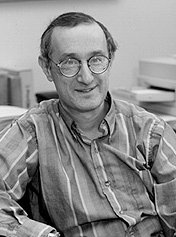
\includegraphics[width=\marginparwidth]{gametheory/axelrod} Robert
%  Axelrod.} 
Such analysis still leaves open the question of which, in practice, is
the optimal strategy for the iterated prisoner's dilemma. In the early
1980's Robert Axelrod performed some experiments on the iterated
prisoner's dilemma \cite{axelrod:84}. He sent out an email asking
people to submit fortran programs that played the prisoner's dilemma
against each other for 200 rounds. The winner was the one that
accumulated the most points.  Many entries were submitted.  They
included the following strategies.

\begin{itemize}
\item \emph{ALL-D}: always play defect.

\item \emph{RANDOM}: pick action randomly. 
  
\item \emph{TIT-FOR-TAT}: cooperate in the first round, then
  do whatever the other player did last time. 
  
\item \emph{TESTER}: defect on the first round. If other player
  defects then play tit-for-tat. If he cooperated then cooperate for
  two rounds then defect.
  
\item \emph{JOSS}: play tit-for-tat but 10\% of the time defect
  instead of cooperating.
\end{itemize}

The \td{tit-for-tat} strategy won the tournament. It still made less
than ALL-D when playing against it but, overall, it won more than any
other strategy. It was successful because it had the opportunity to
play against other programs that were inclined to cooperate. It
cooperated with those that could cooperate and defected against the
rest. This result, while intriguing, is not theoretically robust. For
example a tit-for-tat strategy would lose against a strategy that
plays tit-for-tat but defects on the last round. Still, the
tit-for-tat strategy has been widely used and is considered to be a
simple yet robust strategy.

\medskip

Another method for analyzing repeated games is by assuming that the
players use some learning algorithm and then trying to determine which
strategy their learning will converge to. This research area is known
as learning in games, which we present in
section~\ref{sec:learning-repeated-games}.


%From his tournaments, Axelrod proposes several rules for winning at
%iterated games. He suggests that an 

%\begin{itemize}
%\item \emph{Do not be envious.} You do not need to beat the
%  other guy to do well yourself.
  
%\item \emph{Do not be the first to defect.} This will usually have
%  dire consequences in the long run.
  
%\item \emph{Reciprocate cooperation and defection.} Not just one of
%  them. You must reward and punish, with equal strengths.
  
%\item \emph{Do not be too clever.} Trying to model what the other
%  guy is doing leads you into infinite recursion since he might be
%  modeling you modeling him modeling you.
%\end{itemize}


%Since that tournament there have been many other similar tournaments
%and different variations on the tit-for-tat strategy have won. In
%general we cannot say which is the best strategy because ``best'' is
%defined only relative to whomever else is competing. This fact was
%exploited recently by a team headed by Nick Jennings. \mc{See
%  \hreffoot{http://www.wired.com/news/culture/0,1284,65317,00.html}{``New
%    Tack Win's Prisoner's Dilemma''} by Wendy Grossman, Wired News,
%  2004-10-13.} In this tournament, held in 2004, Jenning's team
%entered a large number of programs. The programs could identify each
%other by issuing a specific sequence of actions. Once they identified
%each other they would recognize if one of them was the ``master''. If
%so, then the other program would always cooperate against the master
%who always defected.  In this way, the master was able to win the
%tournament by exploiting the other programs submitted by Jenning's
%team.

%Axelrod's work was one of the first and among the most well-known
%examples of \td{agent-based modeling} in the social sciences. The idea
%behind agent-based modeling is to build computer models of the
%individual actors then run a program to determine how they will behave
%and how changes in their behavior affect the population as a whole.
%For example, in traditional Economics we consider the aggregate demand
%curves of the whole population against aggregate supply curves. In an
%agent-based model of an economy we would have to implement each
%individual consumer and producer, give them a decision function, and
%run simulations to determine the equilibrium pricing, if any.

%Agent-based modeling is criticized by some who look at the agent
%models and remark that humans do not behave in such simplistic terms
%and our behaviors are too complex to be explained by computer
%programs. Axelrod answers these criticism by noting that his research
%merely provides a \emph{possible} explanation for the emergent
%behavior. That is, the fact that we can build a simulation that uses
%simple agents and has predictive abilities (its results are echoed by
%real-world results) does not necessarily mean that humans use those
%same simple behaviors. However, it does mean that the emergent
%(complex) behaviors observed in the real world can be explained by
%simple agent behaviors. We do not need to resort to complexity at the
%agent level in order to have complexity at the system level.


\section{Games in Extended Form}
\label{sec:games-extended-form}

In \td{extended form} games the players take sequential actions. These
games are represented using a tree where the branches at each level
correspond to a different player's actions and the payoffs to all
agents are given at the leafs. Extended form games can also represent
simultaneous actions by using dotted ellipses to group together nodes
which are equivalent to the rest of the agents because, for example,
they could not see the actions taken by the agent.

\begin{SCfigure}
  \begin{minipage}{1.0\linewidth}
\begin{center}
  \begin{tikzpicture}
    \node[draw,circle,inner sep=.2em,fill=black] (n1) at (0,0) {};
    \node[draw,circle,inner sep=.2em,fill=black] (n2) at (-2,-1) {};
    \node[draw,circle,inner sep=.2em,fill=black] (n3) at (2,-1) {};
    \node[draw,circle,inner sep=.2em,fill=black] (n4) at (-3,-2) {};
    \node[draw,circle,inner sep=.2em,fill=black] (n5) at (-1,-2) {};
    \node[draw,circle,inner sep=.2em,fill=black] (n6) at (1,-2) {};
    \node[draw,circle,inner sep=.2em,fill=black] (n7) at (3,-2) {};
    \draw [->] (n1) -- node[above] {$c$} (n2);
    \draw [->] (n1) -- node[above] {$d$} (n3);
    \draw [->] (n2) -- node[above, near end] {$a$} (n4);
    \draw [->] (n2) -- node[above, near end] {$b$} (n5);
    \draw [->] (n3) -- node[above, near end] {$a$} (n6);
    \draw [->] (n3) -- node[above, near end] {$b$} (n7);
    \draw (-4,-.5) node {Alice}
          (-4,-1.5) node {Bob}
          (-3,-2.5) node {(2,1)}
          (-1,-2.5) node {(2,3)}
          (1,-2.5) node {(3,4)}
          (3,-2.5) node {(4,2)};
    \draw [style=dashed] (0,-1) ellipse (10em and 1em);

  \end{tikzpicture}
\end{center}
  \end{minipage}
  \caption{Game in extended form that corresponds to the normal form
  game from Figure~\ref{fig:stanform}.}
  \label{fig:ext-form}
\end{SCfigure}


Figure~\ref{fig:ext-form} shows the extended form version of the
payoff matrix from figure~\ref{fig:stanform}. In it, the first number
inside the parentheses is the utility that Bob receives and the second
number is Alice's utility.  The dotted line groups together two states
which are invisible to Bob: it shows that Bob does not know the action
Alice took. If we eliminated the dotted line then in that new game
Alice takes an action, which Bob can see, and then Bob takes his
action.

\mc{Extended form games, without the dotted ellipses, are nearly
  identical those built by the minimax algorithm \cite[Chapter
  6]{russell03a}. }

In an extended game a player's strategy $s_i$ is no longer just an
action but can now be a series of actions if the player gets to take
more than one action in the tree, or if the player can have different
actions depending on which node in the tree it is in. That is, if a
player can see others' actions that come before him then his action
can vary. For example, in figure~\ref{fig:ext-form2} a rational Bob
would choose $b$ if Alice has chosen $c$ but would choose $a$ if Alice
has chosen $d$. As before, agent $i$'s utility from strategy $s$ is
given by $u_i(s)$ and corresponds to the values on the leaf node
reached when all players play $s$.


\begin{SCfigure}
  \begin{minipage}{1.0\linewidth}
\begin{center}
  \begin{tikzpicture}
    \node[draw,circle,inner sep=.2em,fill=black] (n1) at (0,0) {};
    \node[draw,circle,inner sep=.2em,fill=black] (n2) at (-2,-1) {};
    \node[draw,circle,inner sep=.2em,fill=black] (n3) at (2,-1) {};
    \node[draw,circle,inner sep=.2em,fill=black] (n4) at (-3,-2) {};
    \node[draw,circle,inner sep=.2em,fill=black] (n5) at (-1,-2) {};
    \node[draw,circle,inner sep=.2em,fill=black] (n6) at (1,-2) {};
    \node[draw,circle,inner sep=.2em,fill=black] (n7) at (3,-2) {};
    \draw [->] (n1) -- node[above] {$c$} (n2);
    \draw [->] (n1) -- node[above] {$d$} (n3);
    \draw [->] (n2) -- node[above, near end] {$a$} (n4);
    \draw [->] (n2) -- node[above, near end] {$b$} (n5);
    \draw [->] (n3) -- node[above, near end] {$a$} (n6);
    \draw [->] (n3) -- node[above, near end] {$b$} (n7);
    \draw (-4,-.5) node {Alice}
          (-4,-1.5) node {Bob}
          (-3,-2.5) node {(2,1)}
          (-1,-2.5) node {(5,4)}
          (1,-2.5) node {(6,3)}
          (3,-2.5) node {(1,2)};
  \end{tikzpicture}
\end{center}
  \end{minipage}
  \caption{Game in extended form.}
  \label{fig:ext-form2}
\end{SCfigure}



\subsection{Solution Concepts}
\label{sec:solution-concepts}

We can apply the Nash equilibrium idea from normal form games to
extended games. Namely, we say that an extended game has a Nash
equilibrium strategy $s^*$ if for all agents $i$ it is true that they
can't gain any more utility by playing a strategy different from
$s^*_i$ given that everyone else is playing $s^*_{-i}$. For example,
for the game in figure~\ref{fig:ext-form2} the Nash equilibrium is
$(c,b)$---Alice plays $c$ and Bob plays $b$. While this strategy is in
equilibrium notice how, if there was some problem or noise in the
system and Alice ends up playing $d$ then Bob's strategy of playing
$b$ is no longer his best response. That is, the basic Nash
equilibrium solution might not be stable under noisy conditions.

A stronger solution concept is the \td{subgame perfect equilibrium}
strategy $s^*$ which is defined as one where for all agents $i$ and
all subgames it is true that $i$ can't gain any more utility by
playing a strategy different from $s^*_i$. We define a subgame to be
any subtree of the extended game. That is, a subgame perfect
equilibrium gives all the agents their best response strategies for
every node in the tree. For example, the subgame perfect equilibrium
for figure~\ref{fig:ext-form2} is for Alice to play $c$ and Bob to
play $b$ if Alice plays $c$ and $a$ if Alice plays $d$.

\medskip

Extended form games are a useful way to represent more complex
multiagent interactions. Notice, however, that they are a special case
of a multiagent Markov decision process. Most researchers have opted
to use the more complete Markov model over the simpler extended form
game for modeling multiagent systems.

These solution concepts provide us with solutions to shoot for when
building multiagent systems, even when these solutions are impossible
to find. For example, say you want to build a team of robot soccer
players. Each robot will have a specific behavior that depends on its
current perception of the world and its internal state. Each robot can
also be assumed to receive a payoff whenever it, or someone in its
team, scores a goal. If you consider the set of all possible agent
behaviors for all agents in the team as the set of actions in a game
then we can talk about the players being at a Nash equilibrium, or
about the players in one team being in the Pareto optimum given the
other team's behaviors. Of course, such equilibria are impossible to
calculate but they do give us a precise goal, of the intellectual
kind, to shoot for. Also, as many researchers have done, we can try to
break up that immense problem into smaller problems for which the
agents can find equilibrium strategies.

\section{Finding a Solution}

There is an extensive literature on centralized algorithms for finding
the various equilibrium strategies for a given game they are, however,
generally considered to be outside the purview of multiagent research.
Generally, the algorithms involve a complete search using heuristics
for pruning.  The \td{Gambit} software program \cite{mckelvey06a} is
an open source implementation of several of these algorithms.

However, note that some of these solutions can be found by more
multiagent-friendly distributed algorithms. In
chapter~\ref{cha:learn-mult-syst} we show multiagent learning
algorithms which allow learning agents to converge to Nash and other
equilibria.


\begin{exercises}
\item Prove that a social welfare solution must be Pareto optimal.

\item Show a 2-person standard form game with 3 actions for each
  player in which iterated dominance leads to a unique equilibrium
  strategy.
\item Assume a 2-person standard form game with $x$ actions for each
  player.
  \begin{enumerate}
  \item What is the maximum number of Pareto optimal pure strategies
    that such a game could have?
  \item Assuming that all payoff values are different, what is the
    maximum number of Pareto optimal pure strategies that such a game
    could have?
  \end{enumerate}

\item Find the pure Nash equilibria, and the Pareto optimal solutions
  of the following game:

    \begin{center}
      \renewcommand\arraystretch{1.5}
      \begin{tabular}{cc|c|c|c|}
        &    &\multicolumn{3}{c}{Alice} \\ 
        &      &$d$&$e$&$f$ \\ \cline{1-5}
        \multirow{3}{2em}{Bob}
        & $a$  &1,2 &2,3 &2,3 \\ \cline{2-5}
        & $b$  &4,5 &6,7 &3,4 \\ \cline{2-5}
        & $c$  &5,4 &6,5 &5,6 \\ \cline{2-5}
      \end{tabular}
    \end{center}


\item The battle of the sexes game, seen in figure~\ref{fig:battlesex}, is a
  classic coordination game in which the players must somehow
  coordinate to agree upon one of the Nash equilibria. These
  problems are solved by populations who adopt a \idx{social law}
  after some trial and error adaptation phase. For example, in the US
  people drive on the right side of the rode while in England they
  drive on the left. Both solutions are equally valid.

  \netlogo{coordination} Implement a NetLogo program where each patch
  repeatedly engages in a battle of the sexes game with one of its
  neighbors, chosen at random. Then try to come up with some simple
  adaptation strategy which the agents could use so that the
  population will quickly converge to an equilibrium.

  Simple adaptation strategies for solving this problem exist
  \cite{shoham97a}, as well as for more complex neighborhood
  definitions \cite{delgado02a}.

\item Lets say that in a repeated version of the game of chicken,
  figure~\ref{chicken}, Alice and Bob decided to converge to the
  strategy (Swerve, Swerve). Since this strategy satisfies the
  maxmin criteria (check this) the Folk theorem tells us that is will
  be stable since both players could play an iterated strategy that
  penalizes the other so that any gains from defection are erased
  after some rounds. Write the short algorithm which describes the
  player's iterated strategy for this situation, that is, the iterated
  strategy they must use to guarantee that (Swerve, Swerve) is the
  equilibrium strategy on every step of the iterated game.

\item A generalization of the Tit-for-Tat strategy is to, instead of
  simply doing exactly what the other agent did last time, make a
  stochastic decision based on the other agent's action. That is, if
  the other agent defected last time then you will be very likely,
  with a given probability, to defect and vice versa. Write a NetLogo
  program where you add these type of agents to a tournament similar
  to Axelrod's. Which strategy triumphs in the end?

  \netlogo{packages} This general strategy is known as
  \idx{reciprocity} and often occurs in human interaction: you are
  more likely, but not entirely sure, to be nice to those that were
  nice to you in the past. Simulations of populations with various
  numbers of reciprocating agents have shown that populations of
  reciprocating agents tend to do better as a whole (since they help
  each other) but can be exploited by selfish agents. This
  exploitation can be curbed by having the reciprocating agents share
  their opinions of other \cite{sen02b}.

\end{exercises}


\chapter{Characteristic Form Games and Coalition Formation}
\label{sec:games-char-form}

There is another type of game studied in game theory: the
\td{characteristic form} game or \td{coalition} game
\cite{osborne99a}. In these games the agents decide how to form
coalitions among themselves and each coalition receives some utility.
For example, a group of people, each with different skills, all want
to start new companies.  The problem they face is deciding how to
divide themselves into subgroups such that each subgroup has the
needed set of skills to succeed in the marketplace.  Similarly, a
group of agents with different skills must decide how to divide itself
into subgroups so as handle as many tasks as possible in the most
efficient manner. Because the agents must cooperate with each other in
order to form coalitions and an agent cannot unilaterally decide that
it will form a coalition with a second agent, these games are known as
\td{cooperative games}. Multiagent researchers have also extended the
basic characteristic form into to the more general coalition
formation, which we also present in this chapter.

It is interesting to note that most game theory textbooks focus
exclusively on non-cooperative games as these have found many
applications in Economics and Business and have been the focus of most
of the research. However, when building multiagent systems we find
that cooperative games are much more useful since they clearly and
immediately model the problem of which agents should perform which
tasks.

\section{Characteristic Form Games}
\label{sec:char-form-games}

Formally, a game in characteristic form includes a set $A =
\{1,\ldots, |A|\}$ of agents. The agents are assumed to deliberate and
the final result of the deliberation is an \td{outcome} $\vu =
(u_1,\ldots,u_{|A|}) \in \Re^{|A|}$ which is just a vector of
utilities, one for each agent. There is also a rule $V(\cdot)$ that
maps every coalition $S \subset A$ to a utility possibility set, that
is $V(S) \subset \Re^{|S|}$. Notice that $V(S)$ returns a set of
utility vectors, not a single utility vector. As such, $V(\cdot)$
provides us the set of payoffs that players in $S$ can achieve it they
form a coalition. For example, for the players $\{1,2,3\}$ we might
have that $V(\{1,2\}) = \{(5,4),(3,6)\}$ meaning that if agents 1 and
2 formed a coalition they could either get 5 for agent 1 and 4 for
agent 2, or they could get 3 for agent 1 and 6 for agent 2. The
function $V$ must be defined for all subsets of $A$.

A special case of the characteristic form game--the one nearly all
multiagent research focuses on---is the \td{transferable utility} game
in characteristic form. This game assumes that the players can
exchange utilities among themselves as they see fit. For example, if
the utility payments are in the form of money then we only need to
specify the total amount of money the coalition will receive and
decide later how this money will be distributed among the agents in
the coalition.  More formally, we define a transferable utility game

\begin{definition}[Tranferable utility characteristic form game] These
  games consist of a set of agents $A = \{1,\ldots,A\}$ and a
  \emph{characteristic function} $v(S) \rightarrow \Re$ defined for
  every $S \subseteq A$.
\end{definition}

The \td{characteristic function} $v(S)$ is also sometimes simply
referred to as the \td{value function} for the coalitions.
Characteristic form games with transferable utility can represent many
multiagent scenarios. For example, they can represent a task
allocation problem where a set of tasks has to be performed by a set
of agents, subsets of whom can sometimes improve their performance by
joining together to perform a task. They can represent a sensor
network problems where the sensors must join together in subgroups to
further refine their readings or relay important information, or they
can represent workflow scheduling systems where agents must form
groups to handle incoming workflows.

\subsection{Solution Concepts}

As is often the case in game theory, there is no clear best solution
to all characteristic form games. Instead, various solutions concepts
have been proposed each one having its own advantages and
disadvantages.

Before defining the solution concepts, we must first notice that the
outcome as we have defined it allows for impossible utility values in
the transferable utility game. Specifically, there might not be a set
of coalitions such that, given $v$, the agents can all get their
utility as promised by \vu{}. In order to rectify this problem we
first specify that we are only interested in \td{feasible} outcomes,
that is, those that can be implemented given $v$.

\begin{definition}[Feasible]
  An outcome $\vu$ is \emph{feasible} if there exists a set of
  coalitions $T = S_1,\ldots,S_k$ where $\bigcup_{S \in T} S = A$
  such that $\sum_{S \in T} v(S) \geq \sum_{i \in A} \vu_i$.
\end{definition}

That is, an outcome $\vu$ is feasible if we can find a disjoint set of
coalitions whose values are as much as that in $\vu$, so we can payoff
$\vu$ with $v$. The set of disjoint coalitions $T$ defined above is
also often referred to as a \td{coalition structure}, also sometimes
represented with the symbol $CS$.

Notice that, if the characteristic function is super-additive then we
can check if an outcome \vu{} is feasible by simply ensuring that
\begin{equation}
  \label{eq:gt-7}
  \sum_{i \in A} \vu_i = v(A).
\end{equation}
We define a \td{super-additive} domain as one where, for all pairs of
disjoint coalitions $S,T \subset A$, we have that $v(S \cup T) \geq
v(S) + v(T)$. That is, there is nothing to be lost by merging into a
bigger coalition. Unfortunately, multiagent systems are rarely
supper-additive since agents have a habit of getting into each others'
way, so that a team is not always better than letting each agent work
on a task separately.

\begin{SCfigure}
  \begin{minipage}{1.0\linewidth}
  \begin{center}
    \begin{tikzpicture}
      \node (n1) at (0,1.5) {\snugbox{$(1)(2)(3)$\\$2 + 2 + 4 =8$}};
      \node (n2) at (-3,0) {\snugbox{$(1)(23)$\\$2 + 8 = 10$}};
      \node (n3) at (0,0) {\snugbox{$(2)(13)$\\$2 + 7 = 9$}};
      \node (n4) at (3,0) {\snugbox{$(3)(12)$\\$4 + 5 = 9$}};
      \node (n5) at (0,-1.5) {\snugbox{$(123)$\\$9$}};
      \node (v) at (-6,0){
        \begin{tabular}{cr} \toprule
          $S$ & $v(S)$ \\ \midrule
          $(1)$ & \emph{$2$} \\ 
          $(2)$ & \emph{$2$}\\ 
          $(3)$ & \emph{$4$}\\ 
          $(12)$& \emph{$5$}\\ 
          $(13)$& \emph{$7$}\\ 
          $(23)$& \emph{$8$}\\ 
          $(123)$& \emph{$9$}\\ \bottomrule
        \end{tabular}};
    \end{tikzpicture}
  \end{center}
  \end{minipage}
  \caption{Sample characteristic form game with transferable utility
    for three agents: 1, 2 and 3.  The table on the left shows the
    values of each coalition. On the right are the coalition
    structures. Below each one we calculate its value.}
  \label{fig:ex1}
\end{SCfigure}
The problem of finding feasible solutions can best be illustrated with
an example.  Figure~\ref{fig:ex1} shows a sample transferable utility
game for three agents along with the definition of the $v$ function
and all possible coalition formations. In this game the outcome $\vu =
\{5,5,5\}$ is not feasible since there is no way to divide the agents
into subsets such that they can all get their utility. If we tried the
coalition $(123)$ then we only have a value of 9 to distribute and we
need a total of 15. On the other hand, the outcome $\vu = \{2,4,3\}$,
is feasible because the coalition structures $(1)(23)$, $(2)(13)$, and
$(123)$ can satisfy it (but not the other ones). However, $\vu =
\{2,4,3\}$ does have a problem in that in it agent 3 is getting an
utility of 3 while we have that $v((3)) = 4$. That is, agent 3 could
defect any one of the three coalition structures we found, join the
coalition $(3)$, and get a higher utility than he currently has. This
outcome thus seems unstable.

\subsubsection{The Core}

%Add simplex graph to show outcomes in the core.

In general, we say that an outcome $\vu$ is stable if no subset of
agents gets paid more, as a whole, than what they get paid in $\vu$.
Stability is a nice property because it means that the agents do not
have an incentive to go off into their own coalition. Our first
solution concept, the \td{core}, refers to all the outcomes that are
stable.

\begin{definition}[Core]
  \label{def:core}
  An outcome $\vu$ is in the \emph{core} if
  \begin{enumerate}
  \item     \[\forall_{S \subset A}: \sum_{i \in S} \vu_i \geq v(S)\]
  \item it is feasible.
  \end{enumerate}
\end{definition}
The first condition in this definition tells us that the utility the
agents receive in outcome $\vu$ is bigger than those of any coalition,
for the agents in the coalition. In other words, that there is no
coalition $S$ whose $v(S)$ is bigger than the sum of payments the
agents in $S$ get under $\vu$. The second condition merely checks that
the total utility we are giving out is not more than what is coming in
via $v(\cdot)$.

\begin{SCfigure}
  \begin{minipage}{1.0\linewidth}
  \begin{center}
    \begin{tikzpicture}
      \node (n1) at (0,1.5) {\snugbox{$(1)(2)(3)$\\$1 + 2 + 2 =5$}};
      \node (n2) at (-3,0) {\snugbox{$(1)(23)$\\$1 + 4 = 5$}};
      \node (n3) at (0,0) {\snugbox{$(2)(13)$\\$2 + 3 = 5$}};
      \node (n4) at (3,0) {\snugbox{$(3)(12)$\\$2 + 4 = 6$}};
      \node (n5) at (3,-1.5) {\snugbox{$(123)$\\$6$}};

      \node (v) at (-6,0){
        \begin{tabular}{cr} \toprule
          $S$ & $v(S)$ \\ \midrule
          $(1)$ & \emph{$1$} \\ 
          $(2)$ & \emph{$2$}\\ 
          $(3)$ & \emph{$2$}\\ 
          $(12)$& \emph{$4$}\\ 
          $(13)$& \emph{$3$}\\ 
          $(23)$& \emph{$4$}\\ 
          $(123)$& \emph{$6$}\\ \bottomrule
        \end{tabular}};

      \node (u) at (-1,-2){
        \begin{tabular}{cr} \toprule
          $\vu$ & in Core? \\ \midrule
          $\{2,2,2\}$ & \emph{yes} \\ 
          $\{2,2,3\}$ & \emph{no} \\ 
          $\{1,2,2\}$ & \emph{no} \\ \bottomrule
        \end{tabular}};
    \end{tikzpicture}
  \end{center}
  \end{minipage}
  \caption{Sample game showing some outcomes that are
    in the core and some that are not. The characteristic function
    $v$ is super-additive.}
  \label{fig:ex2}
\end{SCfigure}


\mpic{gametheory/shapley}{Lloyd F. Shapley}{1923}{}{Responsible for
  the core and Shapley value solution concepts.}  Figure~\ref{fig:ex2}
shows a new game with different payments and a list of outcomes some
of which are in the core and some which are not.  $\{2,2,2\}$ is in
the core because it is feasible and there is no subset of agents $S$
with a $v(S)$ that is bigger than what they could get in this outcome.
$\{2,2,3\}$ is not in the core because it is not feasible. This
outcome adds up to 7 and there is no coalition structure that adds up
to 7. Note that, since the $v$ is super-additive, all we need to check
is the grand coalition. Finally, $\{1,2,2\}$ is not in the core
because agents 1 and 2 are getting a total of 3 while if they formed
the coalition $(12)$ they would get a utility of 4.

We like the core because we know that any solution that is in the core
cannot be improved by having any of the $2^A$ subsets of agents form a
coalition of higher value than they are getting now. It is a very
stable solution. Unfortunately, there are many games with empty cores.
Figure~\ref{fig:emptycore} shows one such example. Try to find an
outcome in the core for this example. You will see that every outcome
is blocked by some other outcome.

\begin{SCfigure}
  \begin{minipage}{1.0\linewidth}
  \centering
  \begin{tabular}{cr} \toprule
    $S$ & $v(S)$ \\ \midrule
    $(1)$ & \emph{$0$} \\ 
    $(2)$ & \emph{$0$}\\ 
    $(3)$ & \emph{$0$}\\ 
    $(12)$& \emph{$10$}\\
    $(13)$& \emph{$10$}\\
    $(23)$& \emph{$10$}\\
    $(123)$& \emph{$10$}\\ \bottomrule
  \end{tabular}
  \end{minipage}
  \caption{Set of payments for a game with an empty core}
  \label{fig:emptycore}
\end{SCfigure}

% \cite{sandholm97b} defines a bounded rational core where there is a
% cost associated with calculating $v(s)$.

Another problem with the core solutions is that when it is not empty
then there are often many outcomes in the core. For example, in
figure~\ref{fig:ex2} any outcome $\vu = \{x,y,z\}$ where $x + y + z
\leq 6$ and $x + y \geq 4$ and $x + z \geq 3$ and $y + z \geq 4$ is in
the core. Thus, we still have a coordination or negotiation problem
where we must choose between these coalitions. Finally, there is the
fact that the outcome does not tell us which coalitions are
formed. For example, if we choose the outcome $\vu = \{2,2,2\}$ then
we must still also choose a coalition structure as there are two
which would work: $(123)$ and $(12)(3)$.


\subsubsection{The Shapley Value}

While the core gives us one possible solution, it suffers from the
fact that many games don't have any solutions in the core and from its
lack of guidance in fairly distributing the payments from a coalition
to its members. The Shapley value solves these problems by giving us
one specific set of payments for coalition members, which are deemed
fair.

\begin{SCfigure}
  \begin{minipage}{1.0\linewidth}
  \centering
  \begin{tabular}{cr} \toprule
    $S$ & $v(S)$ \\ \midrule
    $()$ & \emph{$0$} \\ 
    $(1)$ & \emph{$1$} \\
    $(2)$ & \emph{$3$}\\ 
    $(12)$& \emph{$6$}\\ \bottomrule
  \end{tabular}
  \end{minipage}
  \caption{Example game. If the agents form coalition $(12)$ then how
    much utility should each one get?}
  \label{fig:ex3}
\end{SCfigure}


The problem with identifying fairness in characteristic form games is
best illustrated by an example. Figure~\ref{fig:ex3} shows a game for
two players. Clearly, we should choose the coalition $(12)$ as it has
the highest value. Now we must decide how much each agent should get.
The simplest solution is to divide the total of 6 evenly amongst the
coalition members, so that each agent gets 3. This seems unfair to
agent 2 because agent 2 could have gotten 3 by simply staying on its
own coalition $(2)$. It seems like the fair thing to do is to give
each agent a payment that is proportional to the value it contributes
to the coalition, that is, the amount that value increases by having
the agent in the coalition. But, how do we extend this idea to cases
with more than 2 agents?

Shapley was able to extend this idea by realizing that each agent
should get a payment that corresponds to its marginal contribution to
the final value. An agent's marginal contribution to a coalition is
the difference between the value before the agent joins the coalition
and after he joined. For example, if before you join Initech their
annual profits are \$10M but after you are there for a year they
increase to \$11M then you can claim that your marginal contribution
is to Initech is \$1M assuming, of course, that everything else stays
the same during that year.

The one remaining problem is that there are many different orderings
in which $n$ agents could have joined the coalition, namely, there are
$n!$ orderings of $n$ elements. The \td{Shapley value} simply averages
over all possible orderings. That is, the Shapley value gives each
agent a utility proportional to its average marginal contribution to
every possible coalition, in every possible order it could have been
formed. More formally, we define the Shapley value as:

\begin{definition}[Shapley Value]
  Let $B(\pi,i)$ be the set of agents in the agent ordering $\pi$
  which appear before agent $i$. The \emph{Shapley value} for agent $i$
  given $A$ agents is given by
  \[ \phi(A,i) = \frac{1}{A!} \sum_{\pi \in \Pi_A} v(B(\pi,i) \cup i) -
  v(B(\pi,i)), \]
  where $\Pi_A$ is the set of all possible orderings of the set
  $A$. Another way to express the same formula is 
  \[ \phi(A,i) = \sum_{S\subseteq A} \frac{(|A|-|S|)! \,(|S| - i)!}{|A|!}
  [v(S) - v(S - \{i\})].\]
\end{definition}

Notice that the Shapley values are calculated for a particular
coalition $A$ in the definition above. They are not meant as a way of
determining which is the best coalition structure. They can only be
used to distribute the payments of a coalition once it is formed.

Lets calculate the Shapley values for the game in figure~\ref{fig:ex3}
and the grand coalition $(12)$. Since there are only two agents it
means that there are only two possible orderings: $(12)$ and $(21)$.
As such we have that

\begin{eqnarray*}
  \phi(\{1,2\}, 1) &=&\frac{1}{2}\cdot \left( v(1) - v() + v(21) -
    v(2)\right)\\
  &=&\frac{1}{2}\cdot( 1 - 0 + 6 - 3) = 2 \\
  \phi(\{1,2\}, 2) &=&\frac{1}{2}\cdot \left( v(12) - v(1) + v(2) -
    v()\right)\\
  &=&\frac{1}{2}\cdot( 6 - 1 + 3 - 0) = 4
\end{eqnarray*}
A somewhat surprising and extremely useful characteristic of the
Shapley value is that it is always feasible. In our example the
payments of 4 and 2 add up to 6 which is the same value we get in the
grand coalition $(12)$.  Another nice feature of the Shapley value is
that it always exists and is unique. Thus, we do not have to worry
about coordination mechanism to choose among different payments. A
final interesting result is that the Shapley value might not be in the
core, even for cases where the core exists. This is a potential
problem as it means that the resulting payments might not be stable
and some agents might choose to leave the coalition in order to
receive a higher payment on a different coalition.

%mas-colell glove market, p681

Unfortunately, while the Shapley value has some very attractive
theoretical properties, it does have some serious drawbacks when we
try to use it for building multiagent systems. The biggest problem is
computational. The Shapley value requires us to calculate at least
$2^{|A|}$ orderings, this is only possible for very small sets $A$. It
also requires that we know the value of $v$ for every single subset
$S$.  In many real-world applications the calculation of $v$ is
complex. For example, it might require simulating how a particular
coalition of agents would work together. These complex calculations
could dramatically increase the total time. Finally, the Shapley value
does not give us the actual coalition structure. Thus, it only solves
the second part of the coalition formation problem. We must still
determine which coalition the agents will form and how they will do
it.

\subsubsection{The Nucleolus}
\label{sec:nucleolus}

Since the core is often empty, researchers started looking for ways of
relaxing it and find a new solution concept that would exist for every
game. The problem with the core is that it says that there is no
subset of agents that could get paid more than what they are currently
getting paid in $\vu$, because then they would be tempted to
defect and form a new coalition. If it is impossible to find such an
$\vu$ then the next best thing would be to find the
$\vu$ that minimizes the total temptation felt by the agents.
That is what the \td{nucleolus} aims to do.

We start by clarifying what we mean by temptation. Specifically, a
coalition $S$ is more tempting the higher its value is over what the
agents get in $\vu$. This is known as the \td{excess}.
\begin{definition}[excess]
  The \emph{excess} of coalition $S$ given outcome \vu{} is
  given by 
  \[e(S,\vu) = v(S) - \vu(S), \]
  where 
  \[\vu(S) = \sum_{i\in S} \vu_i.\]
\end{definition}

That is, a coalition $S$ has a positive excess, given \vu{}, if the
agents in $S$ can get more from $v(S)$ than they can from \vu{}. The
more they can get from $S$ the higher the excess. Note that, by
definition, if an outcome \vu{} is in the core then all coalitions
have a excess that is less than or equal to 0 with respect to that
outcome.  But, since we are now concerned with outcomes that are not
in the core we will instead look for those with minimal excess. Since
excess is defined for all possible subsets $S$ we first need a way to
compare the excesses of two outcomes. We do this by putting them in a
sorted list and comparing the list. The one with the higher excess
first is declared more excessive. More formally, for each \vu{} we
find its excess for all subsets $S$ and order these in a list; the
higher excesses come first, as such
\begin{equation}
  \label{eq:gt-8}
  \theta(\vu) = \langle e(S_1^{\vu},\vu), e(S_2^{\vu},\vu),\ldots
  ,e(S_{2^{|A|}}^{\vu},\vu) \rangle,
\end{equation}
where $e(S_i^{\vu}, \vu) \geq e(S_j^{\vu}, \vu)$ for all $i < j$.  We
then define a lexicographical ordering $\succ$ over these lists where
$\theta(\vu) \succ \theta(\vv)$ is true when there is some number $q
\in 1\ldots 2^{|A|}$ such for all $p < q$ we have that
$e(S_p^{\vu},\vu) = e(S_p^{\vv},\vv)$ and $e(S_q^{\vu},\vu) >
e(S_q^{\vv},\vv)$ where the $S_i$ have been sorted as per $\theta$.
That is, if $\theta(\vu) \succ \theta(\vv)$ then that means that when
we sort their excesses for all subsets their first, and greatest,
excesses are all the same and on the first set for which they have a
discrepancy \vu{} has the highest excess. For example, if we had the
lists $\{(2,2,2), (2,1,0), (3,2,2), (2,1,1)\}$ they would be ordered
as $\{(3,2,2), (2,2,2), (2,1,1), (2,1,0)\}$.

We can now define the \td{nucleolus} as the \vu{} which is not
lexicographically bigger than anyone else.
\begin{definition}[nucleolus]
  The \emph{nucleolus} is the set
  \[ \{\vu{} \,|\, \theta(\vu) \not{\succ} \theta(\vv) \text{ for all }
  \vv \text{, given that } \vu \text{ and } \vv \text{ are feasible.}\}\]
  
\end{definition}
In other words, the outcomes in the nucleolus are those where the
excesses for all possible sets are lexicographically not greater than
those of any other outcome. A nice feature of the nucleolus is that it
is always unique for each coalition structure. That is, given a
coalition structure there is only one nucleolus.

The nucleolus captures, to some degree, the idea of an outcome that
minimizes the temptation the agents face. However, notice that the
lexicographic order it defines only cares about the first coalition
that has a higher excess, it does not care about the ones after that.
This could lead to a situation where the sum of the excesses from the
nucleolus is actually larger than that of some other outcome. For
example, $(5.0,0,0)$ comes before $(4,3,3,3)$. As such, the nucleolus
does not seem to minimize the sum of temptations.

\subsubsection{Equal Excess}
\label{sec:equal-excess}

Another technique for calculating the agents' payoff, besides the
Shapley value, is called \td{equal excess}. It is an iterative
algorithm where we adjust the payments that the agents expected they
will receive from each coalition that includes them. At each time step
$t$ we let $E^t(i,S)$ be agent $i$'s expected payoff for each
coalition $S$ which includes him. Initially these are set to 0. We
thus let
\begin{equation}
  \label{eq:gt-9}
  A^t(i,S) = \max _{T \neq S} E^t(i,T)  
\end{equation}
be agent $i$'s expected payment from not choosing $S$ and instead
choosing the best alternative coalition. Then, at each time step we
update the players' expected payments using
\begin{equation}
  \label{eq:gt-10}
  E^{t+1}(i,S) = A^t(i,S) + \frac{v(S) - \sum_{j\in S} A^t(j,S)}{|S|}.
\end{equation}

For example, for the value function given in figure~\ref{fig:ex3} we
start with $E^0(1,*)=E^0(2,*)=0$. Then, at time 1 agent 1 can update
$E^1(1,(1)) = 1$ and $E^1(1,(12)) = 3$ and then $A^1(1,(1)) = 3$ and
$A^1(1,(12)) = 1$, while agent 2 updates $E^1(2,(2)) = 3$ and
$E^1(2,(12)) = 3$ and then $A^1(1,(1)) = 3$ and $A^1(1,(12)) = 3$.

It has been shown that this basic algorithm does not always converge
to a fixed point, however, variations of it have been proposed which
do converge, such as \acro{pact} \cite{goradia07b}. In \acro{pact} the
agents calculate their own $E$ values and exchange them with others
under the assumption that agents will not lie about these values. The
algorithm ensures that the process will stop and a solution will be
found.

Notice that equal excess is a procedural solution to the problem so we
do not know which specific outcome the agents will converge to, other
than to say that they will converge to the outcome that is found when
we use equal excess.


% Note that, since the equal excess procedure requires us to know the
% $A$ values of all agents it is a centralized procedure. However, it
% does not seem impossible that we could parallelize this procedure by
% having the agents exchange $A$ values. \mc{Exercise: Give an example
%   when an agent would want to lie.} Unfortunately, in such a scenario
% it would not be in the agents' best interest to tell the truth about
% its current $A$.

% Yet another equilibrium concept is the kernel (Osborne and
% Rubenstein) which is always non-empty.

\subsection{Finding the Optimal Coalition Structure}

As multiagent system designers we often simply want to find the
outcome that maximizes the sum of values. That is, we want to find the
\td{utilitarian} solution. When the characteristic function is
super-additive then the grand coalition will have the highest value
and thus finding the utilitarian solution is trivial. However, if the
characteristic is not super-additive---as is often the case in
multiagent systems---then we will want an algorithm for finding it.
Notice that under this formulation we are no longer interested in the
specific outcome (that is, individual payments to agents) we are now
only interested in finding best coalition structure, ignoring the
problem of dividing up the value of each coalition among its
participants.

\subsubsection{Centralized Algorithm}
\begin{SCfigure}
  \begin{minipage}{1.0\linewidth}
  \begin{center}
    \begin{tikzpicture}[style=dstyle]
%      \useasboundingbox (-5,-1.5) rectangle (5,2);
      \node at (0,2) {$(1)(2)(3)(4)$};

      \node at (-5,1) {$(12)(3)(4)$};
      \node at (-3,1) {$(13)(2)(4)$};
      \node at (-1,1) {$(14)(2)(3)$};
      \node at (1,1) {$(23)(1)(4)$};
      \node at (3,1) {$(24)(1)(3)$};
      \node at (5,1) {$(34)(1)(2)$};

      \node at (-5,0) {$(1)(234)$};
      \node at (-3.33,0) {$(2)(134)$};
      \node (n1) at (-1.67,0) {$(3)(124)$};
      \node at (0,0) {$(4)(123)$};
      \node at (1.67,0) {$(12)(34)$};
      \node at (3.33,0) {$(14)(23)$};
      \node at (5,0) {$(13)(24)$};

      \node (n2) at (0,-1) {$(1234)$};
%      \node[color=gray] (t) at (-4,-2) {All possible coalitions};
%      \draw[color=gray,->] (t) -- (n1);
%      \draw[color=gray,->] (t) -- (n2);
    \end{tikzpicture}
  \end{center}
  \end{minipage}
  \caption{Coalition structure formation possibilities for four
    agents, organized by the number of coalitions.}
  \label{fig:brute}
\end{SCfigure}

One proposed approach is to a perform a complete search of the
complete set of possible coalition structures, but in a specified
order. Figure~\ref{fig:brute} shows all the possible coalition
structures for four agents. Notice that the bottom two rows contain
all possible coalitions. This means that after searching those two
rows we have seen all possible coalitions. If we let $S^*$ be the
value of the highest valued coalition (\emph{not} coalition structure)
found after searching those two rows then we know that the best
coalition structure cannot be more than $A\cdot S^*$. As such, after
searching the bottom two levels we can say that the optimal solution
is no more than $A$ times better than the best solution we have found
thus far.

\begin{SCfigure}
  \begin{minipage}{1.0\linewidth}
  \begin{center}
    \begin{tabular}{cc}\toprule
      Level&Bound \\ \midrule
      $A$  &$A/2$ \\ 
      $A-1$&$A/2$ \\ 
      $A-2$&$A/3$ \\ 
      $A-3$&$A/3$ \\ 
      $A-4$&$A/4$ \\ 
      $A-5$&$A/4$ \\ 
      :    &:  \\ 
      2    &$A$ \\ 
      1    &none  \\ \bottomrule
    \end{tabular} 
  \end{center}
  \end{minipage}
  \caption{Bounds on optimality after searching various levels.}
  \label{fig:bounds}
\end{SCfigure}

Figure~\ref{fig:bounds} shows the bounds that can be calculated after
examining each of the levels in the graph. One simple algorithm
consists of first searching the bottom two levels then continue
searching down from the top level \cite{sandholm99b}. In this way, the
bound from optimal is reduced as indicated in the figure.  Note that
searching the levels in some other order will not guarantee these
bounds. Notice also that the number of coalition structures in the
second level is given by its \td{Stirling} number
\begin{equation}
  \label{eq:stirling}
\text{Stirling}(A,2) = \frac{1}{2} \sum_{i=0}^{1} (-1)^i
\binom{2}{i}(2-i)^A = 2^{A-1} - 1.  
\end{equation}
So it takes exponential time just to search the second level. In
general, the number of coalition structures for all levels is equal to
the Stirling number for that level.

There also exists an algorithm for finding the optimal coalition
structure which has slightly better bounds than the ones we just
presented, but running time remains exponential and unusable for large
number of agents \cite{dang04a}.


\subsubsection{Distributed Algorithm}

While the previous algorithm found the optical coalition structure, it
did so at the expense of a lot of computation and in a centralized
manner. We now look at one possible way of finding a good, but
possibly not optimal, coalition structure in a decentralized manner.

\begin{SCfigure}
  \begin{minipage}{1.0\linewidth}
  \begin{codebox}
    \Procname{$\proc{Find-Coalition}(i)$}
    \li $L_i \gets$ set of all coalitions that include $i$. 
    \li $S_i^* \gets \arg \max_{S \in L_i} v_i(S)$
%    \li $w_i^* \gets v_i(S_i^*)$
    \li Broadcast $S_i^*$ and wait for all other broadcasts, put these
    into $S^*$ set.
    \li $S_{max} \gets \arg \max _{s \in S^*} v_i(s)$ 
    \li \If $i \in S_{\max}$
    \li \Then join $S_{\max}$
    \li \Return
    \End
    \li \For $j \in S_{\max}$
        \li \Do Delete all coalitions in $L_i$ that contain $j$
        \End
    \li \If $L_i$ is not empty 
    \li \Then goto 2
    \End
    \li \Return
  \end{codebox}
  \end{minipage}
  \caption{Distributed algorithm for coalition formation. Each agent
    $i$ must execute this function. We let $v_i(S) =
    \frac{v(S)}{|S|}$}
  \label{fig:dist}
\end{SCfigure}

\netlogo{find-coalition}Figure~\ref{fig:dist} shows a distributed
algorithm for coalition formation \cite{shehory98a}. The agents order
all their possible coalitions based on how much each will get in that
coalition, where each agent $i$ gets $v_i(S) = v(S)/|S|$ if it joins
coalition $S$. The agents then broadcast the name of their best
coalition. The coalition with maximal $v(S)/|S|$ is chosen by the
agents in $S$ who join the coalition and drop out of the algorithm.
The remaining agents take note of the missing agents by eliminating
from consideration all coalitions that include them. The process is
then repeated again with the new set of coalitions.

This is a classic example of a greedy or hill-climbing algorithm. As
such, we know that it might get stuck on a local optima, which might
or might not be the global optimum. Still, the algorithm should
execute very fast as there are at most $A$ steps and each step
involves having each agent examine all the possible coalitions that it
can be participate in.

A slight modification of the algorithm would be to, instead of
broadcasting at each time step we could let the agents meet randomly
and form a coalition if $v_i(s)$ is maximal for all agents in $s$.
Imagine the agents moving around in a space and forming sets whenever
a group of them happen to be close to each other, then forming a
coalition only if that set has a maximal value. This process is
effectively the same as broadcasting except that it eliminates the
need to broadcast at the expense of taking a longer time to converge
\cite{sarne07a}.


\subsubsection{Reduction to Constraint Optimization}
\label{sec:reduct-constr-optim}

We note that the problem of finding the optimal coalition structure
can be reduced to a constraint optimization problem. The basic idea is
that for $n$ agents there will be at most $n$ coalitions as, at worst,
each agent will stay in the individual coalition. Thus, we can imagine
the problem as consisting of $n$ agents each one deciding which of $n$
rooms to go into. The agents are the variables and the rooms are the
domains. The agents in a room form a coalition and empty rooms are
ignored. We set a constraint for each room equal to $- v(s)$ where $s$
is the set of agents that choose that room, or 0 if no agents choose
it.  We then have a constraint optimization problem where we are
trying to the set of values which minimizes the sum of the constraint
violations, thus maximizing the sum of the valuations.

Note that this is a degenerate case of the constraint optimization
problem in that all the $n$ constraints are over all agents. Most
constraint problems exhibit some degree of locality in that
constraints are only over a small subset of the variables. Having all
constraints be over all variables makes this problem harder than
average. Thus this reduction is likely to be only of theoretical
interest.


%\cite{shehory98a} seems to claim that the solution $CS$ found by this
%algorithm is bound by
%\[\frac{v(CS^*)}{v(CS)} \leq \sum_{i=1}^A \frac{1}{i}\] 
%but, I believe the following example contradicts that claim.

%\begin{SCtable}
%  \begin{minipage}{1.0\linewidth}
%    \begin{center}
%    \begin{tabular}{cc}\toprule
%      Coalition &$v(S)$ \\ \midrule
%      (1,2)  	&$2 x - \epsilon$\\ 
%      (1)	&$0$ \\ 
%      (2)	&$x$ \\ \bottomrule
%    \end{tabular}
%  \end{center}
%  \end{minipage}
%  \caption{Counterexample to bound claims.}
%  \label{tab:counter}
%\end{SCtable}
%Let $a = 2$ and the coalitions have the values as shown in
%Table~\ref{tab:counter}. For this case they predict that

%\[\frac{v(CS^*)}{v(CS)} \leq \frac{3}{2} \]

%but the algorithm would find $CS = (2)(1)$ which has $v(CS)
%= x$, while $v(CS) = 2x - \epsilon$ so 

%\[\frac{v(CS^*)}{v(CS)} = \frac{2x - \epsilon}{x} \leq \frac{3}{2} \]

%which, for small $\epsilon$ means that

%\[2 \leq \frac{3}{2}.\]

%I don't believe that we can place a theoretical bound on the quality
%of the solutions found by the \proc{Find-Coalition} algorithm for
%the general case. Perhaps under certain constrained situations, for
%example, if we limit the characteristic function. Other probabilistic
%bounds could be found via experimentation.


\section{Coalition Formation}
\label{sec:coalition-formation}

The \td{coalition formation} problem, as studied in multiagent
systems, extends the basic characteristic form game in an effort to
make it a better match for real world problems. A coalition formation
problem consists of three steps.
\begin{enumerate}
\item Agents generate values for the $v(\cdot)$ function.
\item Agents solve the characteristic form game by finding a suitable
  set of coalitions.
\item Agents distribute the payments from these coalitions to
  themselves in a suitable manner.
\end{enumerate}

Steps 2 and 3 can be thought of as part of the traditional
characteristic form game. The coalition formation definition simply
chooses to split the problem of finding a suitable outcome \vu{} into
two parts: finding the coalitions and then dividing the payments. The
split mirrors the requirements of many application domains. Step 1 is
completely new. It is there because in many domains it is
computationally expensive to determine the value of $v(S)$ for a given
$S$. For example, if the agents are trying to form groups that solve
particular tasks then calculating $v(S)$ requires them to determine
out how well they can perform the task as a group, which requires
considering how all their different skills can be brought to bear and,
in some common scenarios, requires the development of a full plan---an
exponential problem. The approaches at solving step 1 are thus
generally dependent on the domain and do not generalize well.




%In their abstract they say how it is ``up to $10^{379}$ times faster''
%than the other algorithm but that is just silly for they are talking
%about the case with 1000 agents where their algorithm searches about
%$10^{1100}$ coalition structures and the other algorithm searches
%about $10^{1500}$. Since the number of nanoseconds since the Big bang
%is smaller than $10^{100}$, their claim, while true, seems
%ridiculously out of place.
\begin{exercises}

\item Give an example problem in which agents using equal excess and
  reporting their own $E$ values will want to lie about their own $E$
  values.

\item Find the set of core solutions and the Shapley value of the
  grand coalition for the following game:
  \begin{tabular}{cr} \toprule
          $S$ & $v(S)$ \\ \midrule
          $(1)$ & \emph{$1$} \\ 
          $(2)$ & \emph{$2$}\\ 
          $(3)$ & \emph{$3$}\\ 
          $(12)$& \emph{$5$}\\ 
          $(13)$& \emph{$4$}\\ 
          $(23)$& \emph{$5$}\\ 
          $(123)$& \emph{$5$}\\ \bottomrule
        \end{tabular}


\item Say you have robots which live in a 2-dimensional grid and each
  one has a strength given by a number in the set $\{1,2,3,4,5\}$.
  There are boxes in this world, each one of which must be moved to a
  specified destination. The speed with which a set of robots $S$ can
  move a box is given by $1 - 1/\sum_{i \in S} i.\text{strength}$.
  \begin{itemize}
  \item Formulate this problem as a characteristic form game and
    provide a $v(S)$ definition.
  \item Find a good algorithm for calculating the optimal coalition
    structure.
  \end{itemize}

\item Modify the \proc{find-coalition} algorithm from
  figure~\ref{fig:dist} so that instead of the agents broadcasting
  their values they move around randomly in a two-dimensional space.
  After each time step the set of agents in a tile checks if they form
  a maximal coalition, that is, there is no other coalitions that
  gives one of the agents a higher $v_i(S)$ value. If so, they form
  that coalition and leave the game while the rest keep moving.
  Implement this algorithm in NetLogo and check how long it takes to
  find a solution.


\item We can extend the problem of coalition formation and make it
  more realistic by defining the value function over a set of possible
  agent abilities and then giving the agents sets of abilities
  \cite{yokoo05a}. We then face the possibility of an agent pretending
  to be multiple agents, each with a different ability. Why would an
  agent do this? Give an example when an agent benefits from this
  technique.

  Another problem might be agents that fail to mention to others that
  they have certain skills. Why would an agent do this? Give an
  example when an agent benefits from this technique.


\end{exercises}

%\mc{Talk about Pareto solutions, Shubik figure 6.4.}


%%% Local Variables: 
%%% mode: latex
%%% TeX-command-default: "PDFlatex"
%%% TeX-master: "~/wp/mas/mas"
%%% End: 



\chapter{Learning in Multiagent Systems}
\label{cha:learn-mult-syst}


% Shoham has a good unpublished survey article on reinforcement
% learning. Covers nashq, library/Critical.....

Machine learning algorithms have achieved impressive results. We can
write software that processes larger amounts of data than any human
can and which can learn to find patterns that escape even the best
experts in the field. As such, it is only reasonable that at some
point we will want to add learning agents to our multiagent system.
There are several scenarios in which one might want to add these
learning agents.

Many multiagent systems have as their goal the exploration or
monitoring of a given space, where each agent has only a local view of
its own area. In these scenarios we can envision that each agent
learns a map of its world and the agents further share their maps in
order to aggregate a global view of the field and cooperatively decide
which areas need further exploration. This is a form of cooperative
learning.

Another scenario is in competitive environments each selfish agent
tries to maximize its own utility by learning the other agents'
behaviors and weaknesses. In these environments we are interested in
the dynamics of the system and in determining if the agents will reach
a stable equilibrium. At their simplest these scenarios are repeated
games with learning agents.

To summarize, agents might learn because they don't know everything
about their environment or because they don't know how the other
agents behave. Furthermore, the learning can happen in a cooperative
environment where we also want the agents to share their learned
knowledge, or in a competitive environment where we want them to best
each other. We present analysis and algorithms for learning agents in
these various environment.

\section{The Machine Learning Problem}
\label{sec:machine-learning}

Before delving into multiagent learning we first present a high level
view of what we mean by \td{machine learning}. The word ``learning''
as used casually can have many different meanings, from remembering to
deduction, but machine learning researchers have a very specific
definition of the machine learning problem.


The goal of machine learning research is the development of algorithms
that increase the ability of an agent to match a set of inputs to
their corresponding outputs \cite{mitchell97a}. That is, we assume the
existence of a large set of examples $E$. Each example $e \in E$ is a
pair $e = \{a, b\}$ where $a \in A$ represents the input the agent
receives and $b \in B$ is the output the agent should produce when
receiving this input. The agent must find a function $f$ which maps $A
\rightarrow B$ for as many examples of $A$ as possible. For example,
$A$ could be a set of photo portraits, $B$ could be the set
$\{\text{male}, \text{female}\}$, and each element $e$ tells the
program if a particular photo is of a man or of a woman. The machine
learning algorithm would have to learn to differentiate between a
photo of a man and that of a woman.

\begin{SCfigure}
  \begin{minipage}{1.0\linewidth}
  \begin{center}
    \begin{tikzpicture}[style=dstyle]
      \draw[->] (0,0) -- node[below] {Weight} (4.5,0);
      \draw[->] (0,0) -- node[sloped,above] {Speed} (0,4.5);
      \draw (1,1) node (a) {$+$};
      \draw (.2,3.1) node (b) {$+$};
      \draw (1.2,2.3) node (c) {$+$};
      \draw (1.4,.5) node (d) {$+$};
      \draw (2.2,3.7) node {$+$};
      \draw (.2,.3) node {$+$};
      \draw (3.7,.6) node {$+$};
      \draw (2.8,.1) node {$+$};
      \draw (.4,1.9) node {$+$};
      \draw (3,1.9) node (e) {$-$};
      \draw (2.4,2.7) node (f) {$-$};
      \draw (2.7,2.9) node (g) {$-$};
      \draw (3.3,1.1) node (h) {$-$};
      \draw (3.1,1) node (i) {$-$};
      \draw (2.5,2.4) node (j) {$-$};
      \draw (3.6,1.9) node (k) {$-$};
      \draw[rounded corners=8pt,line width=.1pt]
      (2,.2) -- (3,.3) -- (4,1.2) -- (4,4) -- (2,3.5) -- cycle;
      \draw[rounded corners=8pt,line width=.1pt]
      (1.3,1) -- (3,.3) -- (4.5,2.2) -- (3.5,3.2) -- (3,3.5) --
      (1.5,3) -- cycle;
      \draw[rounded corners=4pt,line width=.1pt]
       (2.1,2.9) -- (2.8,3.1) -- node[above,black] {$f_3$} (3.8,1.9) --
       (3.3,.7) -- (3,.7)-- cycle;
       \draw (4.2,3.4) node {$f_1$};
       \draw (4.6,2.2) node {$f_2$};
%      \draw[->] (a) -- +(0,.5);
%      \draw[->] (b) -- +(.5,.5);
%      \draw[->] (c) -- +(0,.5);
%      \draw[->] (d) -- +(.5,.5);
%      \draw[->] (e) -- +(0,.5);
%      \draw[->] (f) -- +(-.5,-.5);
%      \draw[->] (g) -- +(0,.5);
%      \draw[->] (h) -- +(.5,.5);
    \end{tikzpicture}
  \end{center}
  \end{minipage}
  \caption{The machine learning problem. The input set $A$ corresponds
    to the two axis: Weight and Speed. The outputs $B$ are the set
    $\{+,-\}$. The lines represent three possible functions $f$ which,
    in this case, map anything within the lines as a $-$ and anything
    outside as a $+$. Note that all functions have correctly solved
    the learning problem but in different ways.}
  \label{fig:mlp}
\end{SCfigure}


In a controlled test the set $E$ is usually first divided into a
\idx{training set} which is used for training the agent, and a
\idx{testing set} which is used for testing the performance of the
agent. However, in some scenarios it is impossible to first train the
agent and then test it. In these cases the training and testing
examples are interleaved. The agent's performance is assessed on an
ongoing manner.

Figure~\ref{fig:mlp} shows a graphical representation of the machine
learning problem. The learning problem is coming up with a function
that maps all the points in the space to either $+$ or $-$ such that
it will also correctly categorize any new examples that we have not
seen. Our function must, therefore, extrapolate from the examples it
has seen and generalize to all possible instances. That is, machine
learning performs \td{induction} over the set of examples it has seen
in order to categorize all future examples.

Figure~\ref{fig:mlp} shows three different functions, $f_1$, $f_2$,
and $f_3$, each one of which correctly solves the learning problem.
That is, they are all correct inductions since they correctly
categorize all the examples. In fact, there are an infinite number of
such functions. One might wonder which one is the best one to use. We
don't have a general answer to that question. Each learning algorithm,
from reinforcement learning to support vector machines, arrives at one
learned function but the choice is arbitrary. That is, given the same
examples two learning algorithms can learn to perfectly classify them
but still have learned different functions. This effect is known as
the \td{induction bias} of a learning algorithm. It is because of this
induction bias that some learning algorithms appear to perform better
than others in certain domains---their bias coincides with the
implicit structure of the problem. However, we know that in general,
that is, averages over all possible learning problems there is no
learning algorithm that outperforms all others, a fact that has been
formalized by the \td{no free lunch theorem} \cite{wolpert95a}. Still,
in practice we, as designers, do know a lot about any specific problem
to be learned. You should always try to integrate this knowledge into
the learning algorithm you are using.

\medskip

When a learning agent is placed in a multiagent scenario some of the
fundamental assumptions of machine learning are violated. The agent is
no longer learning to extrapolate from the examples it has seen of
fixed set $E$, instead it's target concept keeps changing (the points
in figure~\ref{fig:mlp} keep moving), leading to a \td{moving target
  function} problem \cite{vidal:98a}. In general, however, the target
concept does not change randomly; it changes based on the learning
dynamics of the other agents in the system. Since these agents also
learn using machine learning algorithms we are left with some hope
that we might someday be able to understand the complex dynamics of
these type of systems.

Learning agents are most often selfish utility maximizers. These
agents often face each other in encounters where the simultaneous
actions of a set of agents leads to different utility payoffs for all
the participants. For example, in a market-based setting a set of
agents might submit their bids to a first-price sealed-bid auction.
The outcome of this auction will result in a utility gain or loss for
all the agents. In a robotic setting two agents headed in a collision
course towards each other have to decide whether to stay the course or
to swerve. The results of their combined actions have direct results
in the utilities the agents receive from their actions. However, even
agents that are trying to learn for themselves might find utility in
sharing this knowledge.



\section{Cooperative Learning}
\label{sec:cooperative-learning}

Imagine two robots equipped with wireless communication capabilities
and trying to map an unknown environment. One of the robots could
learn that the red rocks can be moved but the black rocks are too
heavy to move. The robot could communicate this information to the
other one so that it does not have to re-learn it. Similarly, once one
robot has built a map of one area it could send this map to the other
robot. Of course, this scenario assumes that the two robots are
cooperating with each other in order to build the map.

This type of problem is easy to solve when the robots are identical.
In this case they can simply tell each other everything that they
learn knowing that it will be equally applicable to the other one. One
challenge is trying to prevent the robots from telling each other
things the other already knows. The problem gets much harder when the
robots are heterogeneous. For example, one robot might have learned
that the black rocks can be moved using its large arm but the other
robot might not have an arm that large so this knowledge is useless to
him. To solve this problem we need to somehow model the agents'
capabilities so as to allow one agent to determine which parts of his
learned knowledge will be useful to an agent with a different set of
capabilities. To date, there is scant research on general approaches
to the problem of sharing learned knowledge. Most systems that share
learned knowledge among agents, such as \cite{stone00a}, simply assume
that all agents have the same capabilities.


\section{Repeated Games}
\label{sec:learning-repeated-games}

We now focus on the problem of learning in \td{repeated games}
\cite{fudenberg98a}. In these problems we have two players that face
each other repeatedly on the same game matrix, like the one shown in
figure~\ref{fig:gamematrix}, and each one tries to maximize the sum of
its payoffs over time. You will remember that we already saw a
specific version of this problem called the iterated prisoner's
dilemma.

\begin{SCfigure}
  \begin{minipage}{1.0\linewidth}
  \begin{center}
    \renewcommand\arraystretch{1.5}
    \begin{tabular}{cc|c|c|}
      &    &\multicolumn{2}{c}{$j$} \\  & &$c$&$d$ \\ \cline{1-4}
      \multirow{2}{2em}{$i$}
      & $a$  &0,0 & 5,1 \\ \cline{2-4}
      & $b$  &-1,6 & 1,5 \\ \cline{2-4}
    \end{tabular}
  \end{center}
  \end{minipage}
  \caption{Sample two-player game matrix. Agent $i$ chooses from the
    rows and agent $j$ chooses from the columns.} 
  \label{fig:gamematrix}
\end{SCfigure}


The theory of learning in games studies the equilibrium concepts
dictated by various simple learning mechanisms. That is, while the
Nash equilibrium is based on the assumption of perfectly rational
players, in learning in games the assumption is that the agents use
some kind of algorithm. The theory determines the equilibrium strategy
that will be arrived at by the various learning mechanisms and maps
these equilibria to the standard solution concepts, if
possible. Many learning mechanisms have been studied. The most common
of them are explained in the next few sub-sections.

\subsection{Fictitious Play}
\label{sec:fictitious-play}

A widely studied model of learning in games is the process of
\td{fictitious play}. In it agents assume that their opponents are
playing a fixed strategy. The agents use their past experiences to
build a model of the opponent's strategy and use this model to choose
their own action. Given that all agents are using fictitious play we
try to determine if their learning will converge and, if so, to which
strategy.

Fictitious play uses a simple form of learning where an agent
remembers everything the other agents have done and uses this
information to build a probability distribution for the other agents'
expected strategy. Formally, for the two agent case we say that agent
$i$ maintains a weight function $k_i: S_{j} \rightarrow
\mathcal{R}^+$.  The weight function changes over time as the agent
learns. The weight function at time $t$ is represented by $k_i^t$. It
maintains a count of how many times each strategy has been played by
each other player $j$.  When at time $t-1$ opponent $j$ plays strategy
$s_j^{t-1}$ then $i$ updates its weight function with

\begin{equation}
  \label{eq:1}
  k_i^t(s_j) = k_i^{t-1}(s_j) + 
  \left\{
    \begin{array}{ll}
      1 & \mbox{if $s_j^{t-1} = s_j$,} \\
      0 & \mbox{if $s_j^{t-1} \neq s_j$.}
    \end{array}    
  \right.
\end{equation}

Using this weight function, agent $i$ can assign a probability to $j$
playing any of its $s_j \in S_j$ strategies with

\begin{equation}
  \label{eq:2}
  \Pro_i^t[s_j] = \frac{k_i^t(s_j)}{\sum_{\tilde{s}_j \in S_j} k_i^t(\tilde{s}_j)}.
\end{equation}


That is, $i$ assumes $j$ will pick its action \td{stochastically}
given the values in $k_i(s_j)$. Player $i$ then determines the
strategy that will give it the highest expected utility given that $j$
will play each of its $s_j \in S_j$ with probability $\Pro_i^t[s_j]$.
In other words, $i$ determines its best response to a probability
distribution over $j$'s possible strategies.  In effect, $i$ is
assuming that $j$'s strategy at each time is taken from some fixed but
unknown probability distribution.

\begin{SCfigure}
  \begin{minipage}{1.0\linewidth}
  \begin{center}
    \renewcommand\arraystretch{1.5}
    \begin{tabular}{cc|c|c|}
      &    &\multicolumn{2}{c}{$j$} \\  &  &$c$&$d$ \\ \cline{1-4}
      \multirow{2}{1em}{$i$}
      & $a$  &0,0 & 1,2 \\ \cline{2-4}
      & $b$  &1,2 & 0,0 \\ \cline{2-4}
    \end{tabular}
    \hspace{2em}
    \begin{tabular}{ll!{\vrule}cccc}
      $s_i$ & $s_j$ & $k_i(c)$ & $k_i(d)$ & $\Pr_i[c]$ & $\Pr_i[d]$ \\\hline
      $a$  & $c$  & 1 & 0 & 1 & 0 \\
      $b$  & $d$  & 1 & 1 & .5 & .5 \\
      $a$  & $d$  & 1 & 2 & $1/3$ & $2/3$ \\
      $a$  & $d$  & 1 & 3 & $1/4$ & $3/4$ \\
      $a$  & $d$  & 1 & 4 & $1/5$ & $4/5$ 
    \end{tabular}
  \end{center}
  \end{minipage}
  \caption{Example of fictitious play. The matrix is shown above and
    the values at successive times, each on a different row, are
    shown on the table below. The first row corresponds to time
    0. Note that only $i$ is using fictitious play, $j$ plays the
    values as in the $s_j$ column. $i$'s first two actions are
    stochastically chosen.}
  \label{fig:exbr}
\end{SCfigure}

An example of the best response dynamic at work is shown in
figure~\ref{fig:exbr}. Here we see the values for agent $i$ and its
best responses to agent $j$'s action. Note that in this example agent
$j$ is not using best response. Agent $i$ first notices that $j$
played $c$ and thus sets $k_i^1(c) = 1$. It therefore predicts that
$j$ will play $c$ with probability 1 so its best response at time 2 is
to play $b$, as seen in the second row. Agent $j$ then plays $d$ which
makes $i$ have $\Pro_i^1[c] = \Pro_i^1[d] = .5$. Both of $i$'s actions
have the same expected payoff (1) so it randomly chooses to play $b$.
After that, when $j$ plays $d$ again then $i$'s best response is
unequivocally $b$.

Several interesting results have been derived by research in repeated
games. These results assume that all players are using fictitious
play. For example, we know that the Nash equilibrium remains a
powerful attractor.

\begin{theorem}[Nash Equilibrium is Attractor to Fictitious Play] If
  $s$ is a strict Nash equilibrium and it is played at time $t$ then
  it will be played at all times greater than $t$ \cite{fudenberg90a}.
\end{theorem}


Intuitively, we can see that if the fictitious play algorithm leads
all players to play the same Nash equilibrium then, afterward, they
will all increase the probability that all others are playing the
equilibrium because they just saw them play it. Since, by definition,
the best response of a player when everyone else is playing a strict
Nash equilibrium is to play the same equilibrium, then all players
will play the same strategy and the next time. The same holds true for
every time after that. More importantly, Nash is also where we will
converge to.

\begin{theorem}[Fictitious Play Converges to Nash] If fictitious play
  converges to a pure strategy then that strategy must be a Nash
  equilibrium \cite{fudenberg90a}.
\end{theorem}


We can show this by contradiction. If fictitious play converges to a
strategy that is not a Nash equilibrium then this means that the best
response for at least one of the players is not the same as the
convergent strategy. Therefore, that player will take that action at
the next time, taking the system away from the strategy profile it was
supposed to have converged to.

\begin{SCfigure}
  \begin{minipage}{1.0\linewidth}
  \begin{center}
    \renewcommand\arraystretch{1.5}
    \begin{tabular}{cc|c|c|}
      &    &\multicolumn{2}{c}{$j$} \\ 
      &      &$c$&$d$ \\ \cline{1-4}
      \multirow{2}{1em}{$i$}
      & $a$  &0,0 & 1,1 \\ \cline{2-4}
      & $b$  &1,1 & 0,0 \\ \cline{2-4}
    \end{tabular}
    \hspace{2em}
    \begin{tabular}{ll!{\vrule}cccc}
      $s_i$ & $s_j$ & $k_i(c)$ & $k_i(d)$ & $k_j(a)$ & $k_j(b)$ \\\hline
      &   & 1 & 1.5 & 1 & 1.5 \\
      $a$  & $c$  & 2 & 1.5 & 2 & 1.5 \\
      $b$  & $d$  & 2 & 2.5 & 2 & 2.5 \\
      $a$  & $c$  & 3 & 2.5 & 3 & 2.5 \\
      $b$  & $d$  & 3 & 3.5 & 3 & 3.5 
    \end{tabular}
  \end{center}
  \end{minipage}
  \caption{A game matrix with an infinite cycle.}
  \label{fig:cycle}
\end{SCfigure}

An obvious problem with the solutions provided by fictitious play can
be seen in the existence of infinite cycles of actions. An example is
illustrated by the game matrix in figure~\ref{fig:cycle}. If the
players start with initial weights of $k_i^1(c)=1$, $k_i^1(d)= 1.5$,
$k_j^1(a)=1$, and $k_j^1(b)= 1.5$ they will both believe that the
other will play $b$ or $d$ and will, therefore, play $a$ or $c$
respectively. The weights will then be updated to $k_i^2(c)=2$,
$k_i^2(d)= 1.5$, $k_j^2(a)=2$, and $k_j^2(b)= 1.5$. Next time, both
agents will believe that the other will play $a$ or $c$ so both will
play $b$ or $d$. The agents will engage in an endless cycle where they
alternatively play $(a,c)$ and $(b,d)$.  The agents end up receiving
the worst possible payoff.

This example illustrates the type of problems we encounter when adding
learning to multiagent systems. Most learning algorithms can easily
fall into cycles such as this one.  One common strategy for avoiding
this problem is the use of randomness.  Agents will sometimes take a
random action in an effort to exit possible loops and to explore the
search space. It is interesting to note that, as in the example from
figure~\ref{fig:cycle}, it is often the case that the loops the agents
fall in often reflect one of the mixed strategy Nash equilibria for
the game. That is, $(.5,.5)$ is a Nash equilibrium for this game.
Unfortunately, if the agents are synchronized, as in this case, the
implementation of a mixed strategy could lead to a lower payoff.

Games with more than two players require that we decide whether the
agent should learn individual models of each of the other agents
independently or a joint probability distribution over their combined
strategies.  Individual models assume that each agent operates
independently while the joint distributions capture the possibility
that the others agents' strategies are correlated. Unfortunately, for
any interesting system the set of all possible strategy profiles is
too large to explore---it grows exponentially with the number of
agents. Therefore, most learning systems assume that all agents
operate independently so they need to maintain only one model per
agent.

\subsection{Replicator Dynamics}
\label{sec:replicator-dynamics}

Another widely studied learning model in repeated games is
\td{replicator dynamics}.  This model assumes that the fraction of
agents playing a particular strategy will grow in proportion to how
well that strategy performs in the population. A homogeneous
population of agents is assumed. The agents are randomly paired in
order to play a symmetric game, that is, a game where both agents have
the same set of possible strategies and receive the same payoffs for
the same actions. The replicator dynamics model is meant to capture
situations where agents reproduce in proportion to how well they are
doing and is inspired by biological evolution. In fact, the field that
studies these type of solution concepts is known as \td{evolutionary
  game theory} \cite{weibull97a}.

Formally, we let $\phi^t(s)$ be the number of agents using strategy
$s$ at time $t$.  We can then define
\begin{equation}
  \label{eq:3}
  \theta^t(s) = \frac{\phi^t(s)}{\sum_{s'\in S}\phi^t(s')}  
\end{equation}
to be the fraction of agents playing $s$ at time $t$. The expected
utility for an agent playing strategy $s$ at time $t$ is defined as

\begin{equation}
  \label{eq:4}
  u^t(s) = \sum_{s' \in S} \theta^t(s')u(s,s'),
\end{equation}

where $u(s,s')$ is the utility than an agent playing $s$ receives
against an agent playing $s'$. Notice that this expected utility
assumes that the agents face each other in pairs and choose their
opponents randomly. In the replicator dynamics the reproduction rate
for each agent is proportional to how well it did on the previous
step. Thus, the number of agents playing $s$ at the next time step is
given by

\begin{equation}
  \label{eq:5}
  \phi^{t+1}(s) = \phi^t(s)(1 + u^t(s)).
\end{equation}

\netlogo{evolutionarygt}Notice that the number of agents playing a
particular strategy will continue to increase as long as the expected
utility for that strategy is greater than zero. Only strategies whose
expected utility is negative will decrease in population. As such, the
size of a population will constantly fluctuate. However, when studying
replicator dynamics we ignore the absolute size of the population and
focus on the fraction of the population playing a particular strategy.
We are also interested in determining if the system's dynamics will
converge to some strategy and, if so, which one.

In order to study these systems using the standard solution concepts
we view the fraction of agents playing each strategy as a mixed
strategy for the game. Since the game is symmetric we can use that
strategy as the strategy for both players, so it becomes a strategy
profile. We say that the system is in a mixed Nash equilibrium if the
fraction of players playing each pure strategy is the same as the
probability of the corresponding strategy in the mixed Nash
equilibrium.  For a pure equilibrium all players must play that
strategy. For example, if half the agents are playing $a$ and half $b$
then we can consider this a mixed Nash equilibrium where $a$ and $b$
are each played with $.5$ probability.

An examination of these systems quickly leads to the conclusion that

\begin{theorem}[Nash equilibrium is a Steady State]
  Every Nash equilibrium is a steady state for the replicator
  dynamics \cite{fudenberg98a}.
\end{theorem}

We can prove this theorem by contradiction. If an agent had a pure
strategy that would return a higher utility than any other strategy
then this strategy would be a best response to the Nash equilibrium.
If this strategy was different from the Nash equilibrium then we would
have a best response to the equilibrium which is not the equilibrium,
so the system could not be at a Nash equilibrium.

The reverse has also been shown to be true.

\begin{theorem}[Stable Steady State is a Nash Equilibrium]
  A \emph{stable steady state} of the replicator dynamics is a Nash
  equilibrium. A \emph{stable steady state} is one that, after
  suffering from a small perturbation, is pushed back to the same
  steady state by the system's dynamics \cite{fudenberg98a} .
\end{theorem}

These states are necessarily Nash equilibria because if they were not
then there would exist some particular small perturbation which would
take the system away from the steady state.  This correspondence was
further refined to show that

\begin{theorem}[Asymptotically Stable is Trembling-Hand Nash]
  An asymptotically stable steady state corresponds to a Nash
  equilibrium that is trembling-hand perfect and isolated. That is,
  the stable steady states are a refinement on Nash equilibria---only
  a few Nash equilibria are stable steady states \cite{bomze86a}.
\end{theorem}
On the other hand, it is also possible that a replicator
dynamics system will never converge. In fact, there are many examples
of simple games with no asymptotically stable steady states.

While replicator dynamics reflect some of the most troublesome aspects
of learning in multiagent systems some differences are evident. These
differences are mainly due to the replication assumption. Agents are
not usually expected to replicate, instead they acquire the strategies
of others.  For example, in a real multiagent system all the agents
might choose to play the strategy that performed best in the last
round instead of choosing their next strategy in proportion to how
well it did last time. As such, we cannot directly apply the results
from replicator dynamics to multiagent systems. However, the
convergence of the systems' dynamics to a Nash equilibrium does
illustrate the importance of this solution concept as an attractor of
learning agent's dynamics.


% \subsection{Evolutionary Stable Strategies}
% \label{sec:evol-stable-strat}

Within replicator dynamics we can define a new solution concept
inspired by the ``survival of the fittest'' idea from evolution. An
\td{evolutionary stable strategy} (\acro{ess}) is one which, as a
population, defeats any small number of invading mutants. That is, if
everyone in the population plays that strategy then there is no way a
small number of mutants can invade the population and receive greater
utility than the agents there. More formally, we define it as

\begin{definition}[Evolutionary Stable Strategy] An \acro{ess} is an
  equilibrium strategy that can overcome the presence of a small
  number of invaders. That is, if the equilibrium strategy profile is
  $\omega$ and small number $\epsilon$ of invaders start playing
  $\omega'$ then ESS states that the existing population should get a
  higher payoff against the new mixture ($\epsilon\omega' + (1 -
  \epsilon)\omega$) than the invaders.
\end{definition}


\begin{SCfigure}
  \begin{minipage}{1.0\linewidth}
    \begin{center}
      \begin{tikzpicture}[style=dstyle]

\draw (-2,8.66) node[anchor=north west] {
    \renewcommand\arraystretch{1.5}
    \begin{tabular}{cc|c|c|c|}
      &    &\multicolumn{2}{c}{$j$} \\ 
      &      &$a$ & $b$ & $c$ \\ 
      \cline{1-5} \multirow{3}{1em}{$i$}
      & $a$  &1,1 & 2,0 & 0,2 \\ \cline{2-5}
      & $b$  &0,2 & 1,1 & 2,0 \\ \cline{2-5}
      & $c$  &2,0 & 0,2 & 1,1 \\ \cline{2-5}
    \end{tabular}};

\draw[color=gray] (0,0) -- (10,0) -- (5, 8.66) -- cycle;
\draw (0,0) node[anchor=south east] {$a$};
\draw (10,0) node[anchor=south west] {$c$};
\draw (5,8.66) node[anchor=west] {$b$};

\draw[->] (7,5) -- (7.586751345948128,3.9999999999999996);
\draw[->] (1,0) -- (0.55,0);
\draw[->] (4,5) -- (4.436751345948129,5.499999999999999);
\draw[->] (4,0) -- (2.8,0);
\draw[->] (5,4) -- (5.259401076758503,3.9999999999999996);
\draw[->] (6,6) -- (6.4641016151377535,5.3999999999999995);
\draw[->] (6,0) -- (4.8,0);
\draw[->] (5,5) -- (5.386751345948129,4.999999999999999);
\draw[->] (2,2) -- (2.1547005383792515,2.6);
\draw[->] (8,1) -- (7.7273502691896265,0.7);
\draw[->] (6,2) -- (5.754700538379252,1.7999999999999998);
\draw[->] (2,3) -- (2.4820508075688776,3.8999999999999995);
\draw[->] (8,2) -- (8.154700538379252,1.4000000000000001);
\draw[->] (5,8) -- (5.168802153517006,7.999999999999999);
\draw[->] (3,1) -- (2.477350269189626,1.2000000000000002);
\draw[->] (7,2) -- (6.904700538379251,1.6);
\draw[->] (6,5) -- (6.436751345948128,4.5);
\draw[->] (3,0) -- (1.9500000000000002,0);
\draw[->] (6,3) -- (6.082050807568877,2.6999999999999997);
\draw[->] (4,2) -- (3.754700538379252,2.2);
\draw[->] (5,2) -- (4.704700538379251,1.9999999999999998);
\draw[->] (5,7) -- (5.34145188432738,6.999999999999998);
\draw[->] (4,6) -- (4.464101615137755,6.6);
\draw[->] (3,2) -- (2.9047005383792524,2.4000000000000004);
\draw[->] (3,5) -- (3.586751345948129,6);
\draw[->] (2,1) -- (1.7273502691896256,1.2999999999999998);
\draw[->] (4,1) -- (3.3273502691896257,1.1);
\draw[->] (3,3) -- (3.2320508075688767,3.599999999999999);
\draw[->] (1,1) -- (1.0773502691896257,1.4);
\draw[->] (5,1) -- (4.2773502691896255,0.9999999999999999);
\draw[->] (9,1) -- (9.077350269189628,0.6);
\draw[->] (2,0) -- (1.2,0);
\draw[->] (5,0) -- (3.75,0);
\draw[->] (3,4) -- (3.4594010767585033,4.8);
\draw[->] (8,0) -- (7.200000000000001,0);
\draw[->] (7,1) -- (6.477350269189626,0.8);
\draw[->] (4,3) -- (4.082050807568878,3.3);
\draw[->] (7,0) -- (5.949999999999999,0);
\draw[->] (7,3) -- (7.232050807568877,2.3999999999999995);
\draw[->] (7,4) -- (7.459401076758503,3.2);
\draw[->] (5,3) -- (5.0320508075688775,2.999999999999999);
\draw[->] (5,6) -- (5.414101615137755,5.999999999999998);
\draw[->] (6,1) -- (5.327350269189626,0.8999999999999999);
\draw[->] (4,4) -- (4.309401076758503,4.3999999999999995);
\draw[->] (6,4) -- (6.309401076758503,3.5999999999999996);
\draw[->] (8,3) -- (8.482050807568879,2.099999999999999);
\draw[->] (9,0) -- (8.55,0);
      \end{tikzpicture}      
    \end{center}
  \end{minipage}
  \caption{Visualization of the evolution of populations in replicator
  dynamics. The game is shown in the top left.}
  \label{fig:evolutionviz}
\end{SCfigure}

It has further been shown that

\begin{theorem}[\acro{ess} is Steady State of Replicator Dynamics]
  \acro{ess} is an asymptotically stable steady state of the
  replicator dynamics. However, the converse need not be true---a
  stable state in the replicator dynamics does not need to be an
  \acro{ess} \cite{taylor78a}.
\end{theorem}  

This means that \acro{ess} is a further refinement of the solution
concept provided by the replicator dynamics. \acro{ess} can be used
when we need a very stable equilibrium concept.

\medskip

While these convergence theorems are very usefull, it is also the case
that most systems never converge to a fixed point. In these cases we
need a way to visualize the system dynamics. Since replicator dynamics
is deterministic---we know exactly how each population will
evolve---we can plot a map showing how the population will vary over
time. Figure~\ref{fig:evolutionviz} shows a sample game, at the top
left, and its visualization. The triangle is known as a \td{simplex
  plot} and is used for games with three actions. Every point inside
the triangle represents a possible population. The point at the bottom
left is the population where all agents play $a$. Similarly, the top
point is where all agents play $b$. The point in the exact middle of
the triangle represents the population where $1/3$ of the population
play $a$, $1/3$ play $b$, and $1/3$ play $c$. Each arrow starts at
some population and ends at the next population that would evolve from
that one at the next time step. As can be seen, in this specific game
the population can get into cycles and never converge to a fixed
point.

\subsection{The AWESOME Algorithm}
\label{sec:awesome-algorithm}

While fictitious play and replicator dynamics do not always converge
to an equilibrium, one way we can guarantee that agents will converge
to an equilibrium is by having them calculate and play the same
equilibrium strategy upon starting.  Then, if an agent notices that
the others are not playing the agreed upon equilibrium strategy it can
play fictitious play instead. This is the basic idea of the
\td{AWESOME} (Adapt When Everyone is Stationary, Otherwise Move to
Equilibrium) algorithm \cite{conitzer03a,conitzer06a}. That is, if the
other agents appear to be stationary the an \acro{awesome} agent plays
the best response to their strategy. On the other hand, if they appear
to be adapting then the agents retreats to the equilibrium strategy.

The \acro{awesome} algorithm starts by playing the equilibrium
strategy $\pi_i$ and keeping track of the actions each other player
$j$ has played.  Every $N$ rounds (an epoch) it uses these actions to
build a, possibly mixed, strategy $s_j$ for each player $j$. If $s_j$
is the equilibrium strategy $\pi_j$ for all players $j$ then the
algorithm keeps playing the equilibrium strategy. Otherwise, the
algorithm plays the best response to $s_j$. It is easy to see that if
all the other players are \acro{awesome} players then they will play
their equilibrium strategies and will never diverge from it. If, on the
other hand, an \acro{awesome} player is playing against some players
who are, eventually, playing some other fixed strategy then it will
play a best response strategy against those fixed strategies. Notice
how the algorithm implements the reasoning behind the proof of the
folk theorem.

\begin{SCfigure}
  \begin{minipage}{1.0\linewidth}
    \begin{codebox}
      \Procname{$\proc{awesome}$}
      \li $\pi \gets$ equilibrium strategy
      \li \Repeat
      \li $\id{playing-equilibrium} \gets \const{true}$
      \li $\id{playing-stationary} \gets \const{true}$
      \li $\id{playing-equilibrium-just-rejected} \gets \const{false}$
      \li $\phi \gets \pi_i$
      \li $t \gets 0$
      \li \While \id{playing-stationary}
      \li \Do play $\phi$ for $N^t$ times in a row (an epoch)
      \li     $\forall_j$ update $s_j$ given what they played in these
      $N^t$ rounds.
      \li     \If \id{playing-equilibrium}
      \li     \Then  \If some player $j$ has $\max_a(s_j(a),\pi_j(a)) >
      \epsilon_e$
      \li       \Then
                  $\id{playing-equilibrium-just-rejected} \gets
                   \const{true}$
      \li         $\phi \gets$ random action
                \End
      \li     \Else 
                 \If $\id{playing-equilibrium-just-rejected} =
                 \const{false}$ 
      \zi             \>and some $j$ has
                 $\max_a(s_j^{\text{old}}(a), s_j(a)) > \epsilon_s$
      \li        \Then $\id{playing-stationary} \gets \const{false}$
                 \End
      \li        $\id{playing-equilibrium-just-rejected} \gets
      \const{false}$
      \li        $b \gets \arg \max_a u_i(a,s_{-i})$
      \li        \If $u_i(b,s_{-i}) > u_i(\phi,s_{-i}) +
      n|A_i|\epsilon_s^{t+1}\mu$
      \li        \Then $\phi \gets b$
                 \End
              \End
      \li     $\forall_j s_j^{\text{old}} \gets s_j$
      \li     $t \gets t + 1$
          \End
      \End
    \end{codebox}
  \end{minipage}
  \caption{The \proc{awesome} algorithm. Here $\pi$ is the equilibrium
    strategy which has been calculated before the algorithm starts,
    $n$ is the number of agents, $|A_i|$ is the number of actions the
    agent can take, $\mu$ is the difference between the player's best
    and worst possible utility values, and $s_j(a)$ gives the
    probability with which $j$ will play action $a$ under strategy
    $s_j$. Also, $\epsilon_e$ and $\epsilon_s$ must be decreased and
    $N$ must be increased over time using a valid schedule.}
  \label{fig:awesome}
\end{SCfigure}

While the basic idea is simple, in order to prove that the algorithm
will converge some extra complexity had to be added to it. The
algorithm, shown in figure~\ref{fig:awesome}, has two Boolean state
variables \id{playing-equilibrium} which is true when all other agents
played the equilibrium strategy during the last epoch and
\id{playing-stationary} which is true when all the other agents played
a stationary strategy during the last epoch. Also,
\id{playing-equilibrium-just-rejected} is true when
\id{playing-equilibrium} has just been set to false during the last
check. The algorithm plays the same strategy $\phi$ for a whole epoch
and then assesses the situation. If it turns out that either the
players are not stationary or not in equilibrium the algorithm makes a
note of this and changes its state. If the stationarity hypothesis is
rejected then the whole algorithm is re-started again (back to line
2).

In order for the algorithm to always converge, $\epsilon_e$ and
$\epsilon_s$ must be decreased and $N$ must be increased over time
using a schedule where
\begin{enumerate}
\item $\epsilon_s$ and $\epsilon_e$ decrease monotonically to 0,
\item $N$ increases to infinity,
\item $\prod_{t \leftarrow 1,\ldots,\infty} 1 - \frac{\sum_i
    |A_i|}{N^t(\epsilon_s^t)^2} > 0$
\item $\prod_{t \leftarrow 1,\ldots,\infty} 1 - \frac{\sum_i
    |A_i|}{N^t(\epsilon_e^t)^2} > 0$.
\end{enumerate}

Given such a valid schedule, it can be shown that
\begin{theorem}[\proc{awesome} converges]
  With a valid schedule, the \proc{awesome} algorithm converges to
  best response if all the other players play fixed strategies and to
  a Nash equilibrium if all the other players are \proc{awesome}
  players.
\end{theorem}

Notice that the theorem says that, in self play, it converges to a
Nash equilibrium which might be different from the originally agreed
upon equilibrium strategy $\pi$. For example, say the agents agree on a
mixed equilibrium strategy $\pi$ but some of the actions played in
$\pi$ constitute a pure Nash equilibrium. In this case it could happen
that the players end up, by chance, repeatedly playing the actions in
the pure Nash equilibrium during the first epoch. They might then
decide that everybody else is playing a stationary strategy which
constitutes the pure Nash equilibrium. They will then play the best
response to that pure Nash which, we know, is the same pure Nash
equilibrium. As such, they will get stuck in that equilibrium.

The \proc{awesome} algorithm is a simple way to force agents to
converge to a Nash equilibrium while not letting them be exploited by
other agents that are not using the same algorithm. In those cases
where all agents are \proc{awesome} agents then it converges from the
first step. However, it remains to be seen exactly how much it can be
exploited by clever opponents who know the equilibrium it wants to
play but would rather play something else.

\section{Stochastic Games}

In many multiagent applications the agents do not know the payoffs
they will receive for their actions. Instead, they must take random
actions in order to first explore the world so that they may then
determine which actions lead them to the best payoffs. That is, the
agents inhabit a multiagent Markov decision problem.


\subsection{Reinforcement Learning}
\label{sec:reinf-learn}
%This should be in chapter 1 after MDP and Bellman updates.

A very popular machine learning technique for solving these types of
problems is called \td{reinforcement learning} \cite{sutton98a}, a
specific instance of it is known as \td{Q-learning} \cite{watkins92a}.
Reinforcement learning assumes that the agent lives in a Markov
process and receives a reward in certain states. The goal is to find
the right action to take in each state so as to maximize the agent's
discounted future reward. That is, find the optimal policy.

More formally, we define the reinforcement learning problem as given
by an \acro{mdp} (section~\ref{sec:mark-decis-proc}) where the rewards
are given on the edges instead of in the states. That is, the reward
function is $r(s_t,a_t) \rightarrow \Re$. A reinforcement learning
agent must find the policy $\pi^*$ which maximizes his future
discounted rewards \eqref{eq:mod-bestaction}.

\begin{SCfigure}
  \begin{minipage}{1.0\linewidth}
  \begin{codebox}
    \Procname{$\proc{Q-learning}$}
    \li $\forall_{s} \forall_a Q(s,a) \gets 0$; $\lambda \gets 1$;
    $\epsilon \gets 1$      
    \li $s \gets$ current state
    \li \If $\proc{rand()} < \epsilon$ \>\>\>\>\> \Comment Exploration rate
    \li \Then $a \gets $ random action
    \li \Else $a \gets \arg \max_a Q(s,a)$
    \End
    \li Take action $a$
    \li Receive reward $r$
    \li $s' \gets$ current state
    \li $Q(s,a) \gets \lambda (r +  \gamma \max_{a'}Q(s',a')) + (1-\lambda)Q(s,a)$
    \li $\lambda \gets .99 \lambda$
    \li $\epsilon \gets .98 \epsilon$
    \li \Goto 2
  \end{codebox}
  \end{minipage}
  \caption{\proc{Q-Learning} algorithm. Note that the $.99$ and
    $.98$ numbers are domain-dependent and need to be changed for
    each problem to ensure that the algorithm works. With $\epsilon
    \gets 0$ the algorithm is still guaranteed to work, but in
    practice it might take longer to converge.}
  \label{fig:qlearn}
\end{SCfigure}

The reinforcement learning problem can be solved using the
\proc{Q-learning} algorithm shown in figure~\ref{fig:qlearn}.  Here
$\lambda$ is the \td{learning rate} and $\epsilon$ is the
\td{exploration rate}.  Both are always between 0 and 1. The learning
rate guides how heavily we consider new rewards versus old values we
have learned. When $\lambda = 1$ the algorithm completely re-writes
the old $Q(s,a)$ value while when $\lambda = 0$ is completely ignores
any new reward and instead uses the old $Q(s,a)$. The exploration rate
ensures that we do not converge too quickly to a solution. When
$\epsilon = 1$ all the actions taken by the agent are chosen randomly
while when $\epsilon = 0$ all the actions taken maximize the $Q$
values.

\netlogo{qlearning}It has been shown that \proc{Q-learning} will
converge.

\begin{theorem}[\proc{Q-learning} Converges] Given that the learning
  and exploration rates decrease slowly enough, \proc{Q-learning} is
  guaranteed to converge to the optimal policy \cite{watkins92a} .
\end{theorem}

\proc{Q-learning} differs from the value-iteration algorithm, from
figure~\ref{fig:value-iter}, in several respects. In \proc{Q-learning}
the agent takes actions and learns at the same time. Of course, the
agent's initial actions will be completely random as it has not
learned anything about its expected rewards but, as it takes more
actions it learns to choose better actions. Also, the value-iteration
algorithm requires knowledge of the complete transition and reward
functions of the \acro{mdp} while the \proc{Q-learning} algorithm
explores the parts of the \acro{mdp} that it needs. However, to be
sure that it has found the optimal policy, a \proc{Q-learning} agent
will need to visit every state and take every action.

\medskip

The convergence results of \proc{Q-learning} are impressive, but they
assume that only one agent is learning. We are interested in
multiagent systems where multiple agents are learning. In these games
the reward function is no longer a function of the state and the
agent's actions, instead it is a function of the state and all the
agents' actions. That is, one agent's reward depends on the actions
that other agents take, as captured by the multiagent \acro{mdp} we
discussed in section~\ref{sec:mult-mark-decis}. In these multiagent
\acro{mdp}s it might be impossible for a \proc{Q-learning} agent to
converge to an optimal policy.

As we set out to study these multiagent learning problems, the first
thing we need to do is choose a new equilibrium. Under the single
agent problem definition we were simply looking for the policy that
maximizes the agent's discounted rewards. However, when we have
multiple agents we might want to maximize the sum of all agents'
discounted future rewards (social welfare), or we might choose a more
amenable (for convergence) equilibrium such as the \td{Nash
  equilibrium point}.

\begin{definition}[Nash Equilibrium Point] A tuple of $n$ policies
  $(\pi^*_1,\ldots,\pi_n^*)$ such that for all $s \in S$ and $i =
  1,\ldots,n$,
  \[\forall_{\pi_i \in \Pi_i} v_i(s,\pi_1^*,\ldots\pi_n^*) \geq v_i(s,\pi_1^*,\ldots
  \pi_{i-1}^*, \pi_i, \pi_{i+1}^*,\ldots,\pi_n^*), \]
  where $v_i(s,\pi_1^*,\ldots\pi_n^*)$ is the total rewards (value) that
  agent $i$ can expect to receive starting from state $s$ and assuming
  that agents use policies $\pi_1^*,\ldots\pi_n^*$.
\end{definition}
The Nash equilibrium point is a set of policies such that no one agent
$i$ will gain anything by changing its policy from its Nash
equilibrium point strategies to something else.  As with the regular
Nash equilibrium, it has been shown that the Nash equilibrium point
always exists.

\begin{theorem}[Nash Equilibrium Point Exists] Every $n$-player
  discounted stochastic game possesses at least one Nash equilibrium
  point in stationary strategies \cite{hu03a}.
\end{theorem}

\begin{SCfigure}
  \begin{minipage}{1.0\linewidth}
  \begin{codebox}
    \Procname{$\proc{NashQ-learning}$}
    \li $t \gets 0$
    \li $s \gets$ current state
    \li $\forall_{s \in S} \forall_{j \gets 1,\ldots,n} \forall_{a_j \in
      A_j} Q_j^t(s,a_1,\ldots,a_n) \gets 0$
    \li Choose action $a_i^t$
    \li $s \gets s'$
    \li Observe $r_1^t,\ldots,r_n^t;\, a_1^t,\ldots,a_n^t;s'$
    \li \For $j \gets 1,\ldots,n$ 
    \li \Do $Q_j^{t+1} (s, a_1,\ldots,a_n) \gets$
    \zi \>$(1 - \lambda^t) Q_j^{t}
    (s, a_1,\ldots,a_n) + \lambda^t(r_j^t + \gamma \id{NashQ}_j^t(s'))$
    \zi where $\id{NashQ}_j^t(s') =  Q_j^t(s', \pi_1(s')\cdots\pi_n(s'))$
    \zi and $\pi_1(s')\cdots\pi_n(s')$ are Nash EP calculated from $Q$ values
    \End
    \li $t \gets t + 1$
    \li \Goto 4
  \end{codebox}
  \end{minipage}
  \caption{\proc{NashQ-learning} algorithm}
  \label{fig:nashq}
\end{SCfigure}

We can find the Nash equilibrium point in a system where all the
agents use the \td{\proc{NashQ-learning}} algorithm shown in
figure~\ref{fig:nashq}. In this algorithm each agent must keep $n$
$Q$-tables, one for each agent in the population. These tables are
updated in line~7 using a formula similar to the standard
\proc{Q-learning} update formula but instead of using the Q values to
determine future rewards it uses the \id{NashQ} tables. These tables
hold the Q value for every agent given that all agents play the same
Nash equilibrium policy on the multiagent \acro{mdp} game induced by
the current Q values. That is, the algorithm assumes that the
\acro{mdp} is defined by the Q tables it has and then calculates a
Nash equilibrium point for this problem. We thus note that at each
step the each agent must calculate the Nash equilibrium point given
the current $Q$ functions.  This can be an extremely expensive
computation---harder than finding the Nash equilibrium for a game
matrix.

Still, the \proc{NashQ-learning} algorithm is guaranteed to converge
as long as enough time is given so that all state/action pairs are
explored sufficiently, and the following assumptions hold.

\begin{assumption}
  \label{ass1}
  There exists an adversarial equilibrium for the entire game and
  for every game defined by the $Q$ functions encountered during
  learning.
\end{assumption}
Where an adversarial equilibrium is one where no agent has anything to
lose if the other agents change their policies. That is, if the other
agents change their policies from equilibrium then the agent's
expected reward will either stay the same or increase.
\begin{assumption}
  \label{ass2}
  There exists a coordination equilibrium for the entire game and for
  every game defined by the $Q$ functions encountered during learning.
\end{assumption}
Where a coordination equilibrium is one where all the agents receive
the highest possible value. That is, the social welfare solution.

Under these assumptions it can be shown that \proc{NashQ-learning}
converges.

\begin{theorem}[\proc{NashQ-learning} Converges]
  Under assumptions~\ref{ass1} and~\ref{ass2} \proc{NashQ-learning}
  converges to a Nash equilibrium as long as all the equilibria
  encountered during the game are unique \cite{hu03a}.
\end{theorem}

\begin{SCfigure}
  \begin{minipage}{1.0\linewidth}
  \begin{codebox}
    \Procname{$\proc{friend-or-foe}$}
    \li $t \gets 0$
    \li $s_0 \gets$ current state
    \li $\forall_{s \in S} \forall_{a_j \in A_j} Q_i^t(s,a_1,\ldots,a_n) \gets 0$
    \li Choose action $a_i^t$
    \li $s \gets s'$
    \li Observe $r_1^t,\ldots,r_n^t;\, a_1^t,\ldots,a_n^t;\, s'$
    \li $Q_i^{t+1} (s, a_1,\ldots,a_n) \gets$
    \zi \>$(1 - \lambda^t) Q_i^{t} (s, a_1,\ldots,a_n) + \lambda^t(r_i^t + \gamma \id{NashQ}_i^t(s'))$
    \zi \> where $\id{NashQ}_i^t(s') = \max_{\pi \in \Pi(X_1 \times\cdots\times X_k)} \min_{y_i,\ldots,y_l \in Y_1\times\cdots\times Y_l}$
    \zi \>\> $\sum_{x_1,\ldots ,x_k \in X_1\times\cdots\times X_k} \pi(x_1)\cdots\pi(x_k) Q_i(s,x_1,\ldots, x_k,y_1,\ldots y_l)$
    \zi \> and $X$ are actions for $i$'s friends and $Y$ are for the foes.
    \End
    \li $t \gets t + 1$
    \li \Goto 4
  \end{codebox}
  \end{minipage}
  \caption{\proc{friend-or-foe} algorithm. There are $k$ friends
    with actions taken from $X_1,\ldots,X_k$, and $l$ foes with
    actions taken from $Y_1,\ldots,Y_l$. }
  \label{fig:fof}
\end{SCfigure}

These assumptions can be further relaxed by assuming that we can tell
the agent whether the opponent is a ``friend'', in which case we are
looking for a coordination equilibrium, or a ``foe'', in which case we
are looking for an adversarial equilibrium \cite{littman01a}. With
this additional information we no longer need to maintain a $Q$ table
for each opponent and can achieve convergence with only one, expanded,
$Q$ table. The algorithm is thus called the \proc{friend-or-foe}
algorithm and is shown in figure~\ref{fig:fof}.

In the \td{\proc{friend-or-foe}} algorithm the agent $i$ has $k$
friends with action sets represented by $X_1,\ldots,X_k$ and $l$ foes
with action sets represented by $Y_1,\ldots,Y_l$.  The algorithm
implements the idea that $i$'s friends are assumed to work together to
maximize $i$'s value and $i$'s foes are working to minimize it. We can
show that \proc{friend-or-foe} converges to a stable policy. However,
in general these do not correspond to a Nash equilibrium point. Still,
we can show that it often converges to a Nash equilibrium.

\begin{theorem}
  \proc{foe-q} learns values for a Nash equilibrium policy if the game
  has an adversarial equilibrium and \proc{friend-q} learns values for
  a Nash equilibrium policy if the game has a coordination
  equilibrium. This is true regardless of opponent behavior
  \cite{littman01a}.
\end{theorem}


That is, if the game has one of the equilibria and we correctly
classify all the other agents as either friends or foes then the
\proc{friend-or-foe} algorithm is guaranteed to converge.

\proc{friend-or-foe} has several advantages over
\proc{NashQ-learning}. It is does not require the learning of $Q$
functions for each one of the other agents and it is easy to implement
as it does not require the calculation of a Nash equilibrium point at
each step. On the other hand, it does require us to know if the
opponents are friends or foes, that is, whether there exists a
coordination or an adversarial equilibrium.

Neither algorithm deals with the problem of finding equilibria in
cases without either coordination or adversarial equilibria. Such
cases are the most common and most interesting as they require some
degree of cooperation among otherwise selfish agents.

\section{General Theories for Learning Agents}
\label{sec:learning-agents}

The theory of learning in games provides the designer of multiagent
systems with many useful tools for determining the possible
equilibrium points of a system. Unfortunately, most multiagent systems
with learning agents do not converge to an equilibrium. Designers
often use learning agents because they do not know, at design time,
the specific circumstances that the agents will face at run time.  If
a designer knew the best strategy, that is, the Nash equilibrium
strategy, for his agent then he would simply implement this strategy
and avoid the complexities of implementing a learning algorithm.
Therefore, we will see a multiagent system with learning agents when
the designer cannot predict that an equilibrium solution will emerge.

The two main reasons for this inability to predict the equilibrium
solution of a system are the existence of unpredictable environmental
changes that affect the agents' payoffs and the fact that on many
systems an agent only has access to its own set of payoffs---it does
not know the payoffs of other agents. These two reasons make it
impossible for a designer to predict which equilibria, if any, the
system would converge to. However, the agents in the system are still
playing a game for which an equilibrium exists, even if the designer
cannot predict it at design-time. But, since the actual payoffs keep
changing it is often the case that the agents are constantly changing
their strategy in order to accommodate the new payoffs.

As mentioned earlier, learning agents in a multiagent system are faced
with a moving target function problem \cite{vidal:98a}. That is, as
the agents change their behavior in an effort to maximize their
utility their payoffs for those actions change, changing the expected
utility of their behavior. The system will likely have non-stationary
dynamics---always changing in order to match the new goal. While game
theory tells us where the equilibrium points are, given that the
payoffs stay fixed, multiagent systems often never get to those
points.  A system designer needs to know how changes in the design of
the system and learning algorithms will affect the time to
convergence.  This type of information can be determined by using
\acro{clri} theory.

\subsection{CLRI Model}
\label{sec:clri-theory}

The \td{CLRI model} \cite{vidalclri} provides a method for analyzing a
system composed of learning agents and determining how an agent's
learning is expected to affect the learning of other agents in the
system.  It assumes a system where each agent has a decision function
that governs its behavior as well as a target function that describes
the agent's best possible behavior. The target function is unknown to
the agent. The goal of the agent's learning is to have its decision
function be an exact duplicate of its target function. Of course, the
target function keeps changing as a result of other agents' learning.

Formally, the \acro{clri} model assumes that there is a fixed set of
autonomous agents in the system.  The system can be described by a set
of discrete states $s \in S$ which are presented to the agent with a
probability dictated by the fixed probability distribution
$\mathcal{D}(S)$.  Each agent $i$ has a set of possible actions $A_i$
where $|A_i| \geq 2$. Time is discrete and indexed by a variable $t$.
At each time $t$ all agents are presented with a new $s \in
\mathcal{D}(S)$, take a simultaneous action, and receive some payoff.
The scenario is similar to the one used by fictitious play except for
the addition of state $s$.

Each agent $i$'s behavior is defined by a policy $\pi_i^t(s) : S
\rightarrow A$. When $i$ learns at time $t$ that it is in state $s$ it
will take action $\pi_i^t(s)$. At any time there is an optimal policy
for each agent $i$, also known as its target function, which we
represent as $\Pi_i^t(s)$. Agent $i$'s learning algorithm will try to
reduce the discrepancy between $\pi_i$ and $\Pi_i$ by using the
payoffs it receives for each action as clues as clues as to what it
should do given that it does not have direct access to $\Pi_i$. The
probability that an agent will take a wrong action is given by its
error $e(\pi_i^t) = \Pro[\pi_i^t(s) \neq \Pi_i^t(s) \,|\, s
\in \mathcal{D}(S)]$. As other agents learn and change their decision
function, $i$'s target function will also change, leading to the
moving target function problem, as depicted in
figure~\ref{fig:learn-mas}.


\begin{SCfigure}
  \begin{minipage}{1.0\linewidth}
  \begin{center}
    \begin{tikzpicture}[style=dstyle]
      \draw (0,0) node (dt) {$\pi^t_i$};
      \draw (4,0) node (tt) {$\Pi^t_i$};
      \draw[gray] (dt) -- node[below] {\textcolor{black}{$e(\pi_i^t)$}} (tt);
      \draw (1,2) node (dtt) {$\pi^{t+1}_i$};
      \draw[->] (dt) -- node[sloped,above] {Learn} (dtt);
      \draw (6,0) node (ttt) {$\Pi^{t+1}_i$};
      \draw[->] (tt) -- node[below] {Move} (ttt);
      \draw[gray] (dtt) -- node[sloped,above] {\textcolor{black}{$e(\pi_i^{t+1})$}} (ttt);
    \end{tikzpicture}
  \end{center}
  \end{minipage}
  \caption{The moving target function problem.}
  \label{fig:learn-mas}
\end{SCfigure}


% \centelatex-beamer-announce@lists.sourceforge.netrline{
%   \xymatrix{
%     & &  \delta_i^{t+1}  \ar@{~}[rrrrd]^{e(\delta_i^{t+1})}
%     & & & \\
%     \delta_i^t \ar[rru]^{\txt{Learn}} \ar@{~}[rrrrr]_{e(\delta_i^t)} &&
%     & & & \Delta_i^t \ar[r]_{\txt{Move}} & \Delta_i^{t+1}
%   }}


An agent's error is based on a fixed probability distribution over
world states and a Boolean matching between the decision and target
functions. These constraints are often too restrictive to properly
model many multiagent systems. However, even if the system being
modeled does not completely obey these two constraints, the use of the
\acro{clri} model in these cases still gives the designer valuable
insight into how changes in the design will affect the dynamics of the
system.  This practice is akin to the use of Q-learning in
non-Markovian games---while Q-learning is only guaranteed to converge
if the environment is Markovian, it can still perform well on other
domains.

The \acro{clri} model allows a designer to understand the expected
dynamics of the system, regardless of what learning algorithm is used,
by modeling the system using four parameters: Change rate, Learning
rate, Retention rate, and Impact (\acro{clri}). A designer can
determine values for these parameters and then use the \acro{clri}
difference equation to determine the expected behavior of the system.

The change rate ($c$) is the probability that an agent will change at
least one of its incorrect mappings in $\delta^t(w)$ for the new
$\delta^{t+1}(w)$. It captures the rate at which the agent's learning
algorithm tries to change its erroneous mappings. The learning rate
($l$) is the probability that the agent changes an incorrect mapping
to the correct one. That is, the probability that $\delta^{t+1}(w) =
\Delta^t(w)$, for all $w$. By definition, the learning rate must be
less than or equal to the change rate, i.e. $l \leq c$. The retention
rate ($r$) represents the probability that the agent will retain its
correct mapping. That is, the probability that $\delta^{t+1}(w) =
\delta^t(w)$ given that $\delta^t(w) = \Delta^t(w)$.

\acro{clri} defines a volatility term ($v$) to be the probability that
the target function $\Delta$ changes from time $t$ to $t+1$. That is,
the probability that $\Delta^t(w) \neq \Delta^{t+1}(w)$. As one would
expect, volatility captures the amount of change that the agent must
deal with. It can also be viewed as the speed of the target function
in the moving target function problem, with the learning and retention
rates representing the speed of the decision function. Since the
volatility is a dynamic property of the system (usually it can only be
calculated by running the system) \acro{clri} provides an impact
($I_{ij}$) measure. $I_{ij}$ represents the impact that $i$'s learning
has on $j$'s target function. Specifically, it is the probability that
$\Delta_j^t(w)$ will change given that $\delta_i^{t+1}(w) \neq
\delta_i^t(w)$.

Someone trying to build a multiagent system with learning agents would
determine the appropriate values for $c$, $l$, $r$, and either $v$ or
$I$ and then use 

\begin{multline}
  \label{eq:main:simp}
  E[e(\delta_i^{t+1})] = 1 - r_i + v_i
  \left(
    \frac{|A_i|r_i - 1}{|A_i| -1}
  \right) \\
  + e(\delta_i^t)
  \left(
    r_i -l_i + v_i
    \left(
      \frac{|A_i|(l_i - r_i) + l_i - c_i}{|A_i| -1}
    \right)
  \right)
\end{multline}

in order to determine the successive expected errors for a typical
agent $i$. This equation relies on a definition of volatility in terms
of impact given by
\begin{equation}
  \label{eq:16}
  \begin{split}
    \forall_{w \in W} \; v_{i}^{t} &= \Pro[\Delta_i^{t+1}(w) \neq \Delta_i^t(w)] \\
    &= 1 - \prod_{j \in N_{-i}}(1 - I_{ji} \Pro[\delta_j^{t+1}(w) \neq \delta_j^t(w)]), \\
  \end{split}
\end{equation}
which makes the simplifying assumption that changes in agents'
decision functions will not cancel each other out when calculating
their impact on other agents. The difference equation
\eqref{eq:main:simp} cannot, under most circumstances, be collapsed
into a function of $t$ so it must still be iterated over.  On the
other hand, a careful study of the function and the reasoning behind
the choice of the \acro{clri} parameter leads to an intuitive
understanding of how changes in these parameters will be reflected in
the function and, therefore, the system. A knowledgeable designer can
simply use this added understanding to determine the expected behavior
of his system under various assumptions. An example of this approach
is shown in \cite{brooks02a}.

For example, it is easy to see that an agent's learning rate and the
system's volatility together help to determine how fast, if ever, the
agent will reach its target function. A large learning rate means that
an agent will change its decision function to almost match the target
function. Meanwhile, a low volatility means that the target function
will not move much, so it will be easy for the agent to match it.
Thus, if the agents have no impact on each other, that is, $I_{ij} =
0$ for all $i,j$, then the agents will learn their target function and
the system will converge. As the impact increases then it becomes more
likely that the system will never converge.  

Of course, this type of simple analysis ignores a common situation
where the agent's high learning rate is coupled with a high impact on
other agents' target function making their volatility much higher.
These agents might then have to increase their learning rate and
thereby increase the original agent's volatility. Equation
\eqref{eq:main:simp} is most helpful in these type of feedback
situations.


\subsection{N-Level Agents}
\label{sec:n-level-agents}

Another issue that arises when building learning agents is the choice
of a modeling level. A designer must decide whether his agent will
learn to correlate actions with rewards, or will try to learn to
predict the expected actions of others and use these predictions along
with knowledge of the problem domain to determine its actions, or will
try to learn how other agents build models of other agents, etc. These
choices are usually referred to as \td{n-level} modeling agents---an
idea first presented in the recursive modeling method
\cite{gmytrasiewicz95a} \cite{gmytrasiewicz01a}.

A \td{0-level} agent is one that does not recognize the existence of
other agents in the world. It learns which action to take in each
possible state of the world because it receives a reward after its
actions. The state is usually defined as a static snapshot of the
observable aspects of the agent's environment. A \td{1-level} agent
recognizes that there are other agents in the world whose actions
affect its payoff.  It also has some knowledge that tells it the
utility it will receive given any set of joint actions. This knowledge
usually takes the form of a game matrix that only has utility values
for the agent. The 1-level agent observes the other agents' actions
and builds probabilistic models of the other agents. It then uses
these models to predict their action probability distribution and uses
these distributions to determine its best possible action. A
\td{2-level} agent believes that all other agents are 1-level agents.
It, therefore, builds models of their models of other agents based on
the actions it thinks they have seen others take. In essence, the
2-level agent applies the 1-level algorithm to all other agents in an
effort to predict their action probability distribution and uses these
distributions to determine its best possible actions. A 3-level agent
believes that all other agents are 2-level, an so on.  Using these
guidelines we can determine that fictitious play
(section~\ref{sec:fictitious-play}) uses 1-level agents while the
replicator dynamics (section~\ref{sec:replicator-dynamics}) uses
0-level agents.

These categorizations help us to determine the relative computational
costs of each approach and the machine-learning algorithms that are
best suited for that learning problem. 0-level is usually the easiest
to implement since it only requires the learning of one function and
no additional knowledge. 1-level learning requires us to build a model
of every agent and can only be implemented if the agent has the
knowledge that tells it which action to take given the set of actions
that others have taken. This knowledge must be integrated into the
agents. However, recent studies in layered learning \cite{stone00a}
have shown how some knowledge could be learned in a ``training''
situation and then fixed into the agent so that other knowledge that
uses the first one can be learned, either at runtime or in another
training situation. In general, a change in the level that an agent
operates on implies a change on the learning problem and the knowledge
built into the agent.

Studies with n-level agents have shown \cite{vidal:98b} that an
n-level agent will perform better in a society full of (n-1)-level
agents, and that the computational costs of increasing a level grow
exponentially.  Meanwhile, the utility gains to the agent grow smaller
as the agents in the system increase their level, within an economic
scenario. The reason is that an n-level agent is able to exploit the
non-equilibrium dynamics of a system composed of (n-1)-level agents.
However, as the agents increase their level the system reaches
equilibrium faster so the advantages of strategic thinking are
reduced---it is best to play the equilibrium strategy and not worry
about what others might do. On the other hand, if all agents stopped
learning then it would be very easy for a new learning agent to take
advantage of them. As such, the research concludes that some of the
agents should do some learning some of the time in order to preserve
the robustness of the system, even if this learning does not have any
direct results. That is, there appear to be decreasing marginal
returns for strategic thinking.

% Add info on Reasoning about Knowledge book.

\section{Collective Intelligence}
\label{sec:coin}

We can also try to use machine learning as a way to automatically
build multiagent systems where each one of the agents learns to do
what we want. For example, imagine a factory floor with boxes that
need to be moved and robots of different abilities. Depending on the
size and weight of the boxes, different robots, or combinations of
robots, are able to move them. We know that our goal is for all boxes
to be placed against the South wall. Then, rather than trying to come
up with specific plans or rules of behavior for each robot, we instead
install a reinforcement learning algorithm in each one of them and set
them off to learn how best to coordinate. The question we must then
ask is: what is the reward function for each agent? As we saw in the
\acro{clri} model, one agent's actions can have an impact on another
agent's target function thus making it hard, or even impossible, for
the other agent to converge in its learning. For example, if one robot
keeps changing its behavior and moving around randomly then it will be
impossible for another agent to learn to predict when they will both
be in front of a large box so that they can move it together.

Collective intelligence (\td{COIN}) aims to formalize these ideas and
determine what kind of rewards we should provide
reinforcement-learning agents in order to achieve a desired global
behavior \cite{wolpert99a}. Specifically, we are given a global
utility function $U(s,\va) \rightarrow \Re$ which tells us the value
for every vector of actions $\va = \{a_1, a_2,\ldots, a_n\}$ of the
agents and state of the world $s$. The agents are assumed to use some
reinforcement learning algorithm, such as Q-learning. Our problem is
then to define the agents' reward functions $u_i(s, \va)$ such that
the agents will end up with policies $\pi_i^*$ that maximize $U$.
Notice that simply setting $u_i(s, \va) = U(s, \va)$ for all $i$ can
lead to agents receiving an uninformative reward. For example, if a
confused agents throws itself against a wall while, at the same time,
all the other agents cooperate to move the box correctly then the
confused agent will receive a high reward and will thus likely
continue to throw itself against the wall.

Still, in general we do want to align each agent's rewards with the
global utility. We can quantify this alignment by defining agent $i$'s
preference over $s,\va$ as
\begin{equation}
  \label{eq:preference}
  P_i(s,\va) = \frac{\sum_{\va' \in \vA} \Theta[u_i(s,\va) - u_i(s,\va')]}{|\vA|},
\end{equation}
where $\Theta(x)$ is the Heaviside function which is 1 if $x$ is
greater than or equal to 0, otherwise it is 0. Similarly, we can
define the global preference function as
\begin{equation}
  \label{eq:global-pref}
    P(s,\va) = \frac{\sum_{\va' \in \vA} \Theta[U(s,\va) - U(s,\va')]}{|\vA|}.
\end{equation}
Both of these functions serve to rank the agents', or the global,
preferences over the set of all possible states and actions vectors.
For example, if a particular $(s,\va)$ is preferred over all others
then $P(s,\va) = 1$.  

In general, we might want an agent's preferences to be similar to the
system's preferences so that the agent's learning mechanism will try
to converge towards the desired system's preferences. A system where,
for all agents $i$ it is true that $P_i(s,\va) = P(s,\va)$ is called
\td{factored}. These systems are nice in that they provide the correct
incentives to the agents in all situations. Thus, factored systems are
more likely to converge to the set of policies that maximizes $U$. 

It is possible that factored systems might not converge because
agents' action might have an impact on each other thus changing each
other's target function.  This idea is captured within the \acro{coin}
framework as the \td{opacity} of $u_i(s,\va)$. Specifically, we define
the opacity $\Omega_i$ for agent $i$ as
\begin{equation}
  \label{eq:opacity}
  \Omega_i(s,\va) = \sum_{\va' \in \vA} \Pro[\va']
  \frac{|u_i(s,\va) - u_i(s,\va'_{-i},\va_i)|}{|u_i(s,\va) - u_i(s,\va_{-i},\va'_{i})|}.
\end{equation}
The opacity is zero when the agent's rewards are the same regardless
of the actions taken by other, that is, when the other agents' actions
have no impact on what the agent should do. On the other hand, the
opacity gets larger as the other agents' actions change the reward the
agent will get. Just like with the \acro{clri} impact, if the opacity
is zero for all states and action vectors then the multiagent learning
problem is reduced to the single-agent learning problem as the agents
have no effect on each other's target function. More generally, a
decrease in the opacity amounts to an increase in the signal-to-noise
ratio that the agent receives via its reward function.

Systems that are both factored and have zero opacity for all agents
are extremely rare, but would be easy to solve. Systems where the
opacity is zero for all agents amount to multiple learning problems
that do not interfere with each other and are easy to solve, but they
are also very rare. Our goal can now be re-stated as that of finding
reward functions for each agent that have as low opacity as possible
while also being as highly factored as possible.

One solution \acro{coin} proposes is the use of the \td{wonderful
  life} reward function which gives each agent a reward proportional
to its own contribution to the global utility. It implements the same
idea as the \acro{vcg} payments (Chapter~\ref{vcg}). Formally, agent
$i$'s wonderful life reward is given by
\begin{equation}
  \label{eq:wonderful-life}
  u_i(s,\va) = U(s, \va) - U(s,\va_{-i}),
\end{equation}
where the $U(s,\va_{-i})$ represents the utility in state $s$ when
agent $i$ does not exist and all other agents take actions as in
$\va_{-i}$. Notice that this equation can be derived directly from the
global utility function. Thus, it is applicable to any system where we
have a pre-defined utility function $U$. It has been shown that this
reward function performs better than using $u_i = U$ and other
seemingly appropriate reward functions \cite{wolpert99b,tumer04a}.

Another solution is the \td{aristocrat utility}, which is defined as
\begin{equation}
  \label{eq:aristocrat}
  u_i(s,\va) = U(s, \va) - \sum_{\va' \in \vA} \Pro[\va'] U(s,\va_{-i},\va'_i),
\end{equation}
where $\Pro[\va']$ is the probability that $\va'$ happens.
\netlogo{coin} The aristocrat utility measures the difference in the
global utility between the agent's action and its average or expected
action. It has been shown that this reward function also performs
well, sometimes better than the wonderful life utility
\cite{wolpert01a} .


\section{Summary}
% future challenges

We have seen how the theory of learning in games provides us with
various equilibrium solution concepts and often tells us when some of
them will be reached by simple learning models.  On the other hand, we
have argued that the reason learning is used in a multiagent system is
often because there is no known equilibrium or the equilibrium point
keeps changing due to outside forces. We have also shown how the
\acro{clri} theory and n-level agents are attempts to characterize and
predict, to a limited degree, the dynamics of a system given some
basic learning parameters.

\section{Recent Advances}
\label{sec:recent-advances}

The GAMUT \cite{nudelman04a} software can produce game matrices from
thirty-five base classes of games. These matrices can be used to
determine how well learning algorithms perform under all possible game
types and sizes.

\begin{exercises}
  \item In general, which game matrices have cycles for fictitious play?
\end{exercises}


% regret matching, amy greenwald
% \url{http://www.cs.brown.edu/courses/cs295-5/readings/gjm.pdf}

%http://www.mcs.utulsa.edu/~banerjdi/aaai05MALWshop-CJAL.pdf and other
% "Reaching Pareto Optimality in Prisoner's Dilemma Using Conditional
% Joint Action Learning," where if both agents use the given learning
% algorithm they will converge to a Pareto optimal solution.

%Parkes' class
%%http://www.eecs.harvard.edu/~parkes/cs286r/spring06/schedule.html
%has a few papers on MAL.

%Upcoming special issue of Machine Learning
%http://www.cs.rutgers.edu/~mlittman/topics/mlj05-gametheory/
%Learning and Computational Game Theory: 

%A tutorial on MAL
%http://www.cs.rutgers.edu/~mlittman/talks/ijcai03-games/
%A paper on learning-teaching in MAL
%http://www.cs.utexas.edu/~pstone/Papers/bib2html-links/threats-ATAL2001.pdf

%%% Local Variables: 
%%% mode: latex
%%% TeX-command-default: "PDFlatex"
%%% TeX-master: "~/wp/mas/mas"
%%% End: 


\chapter{Negotiation}
\label{cha:negotiation}

A negotiation problem is one where multiple agents try to come to an
agreement or \td{deal}. Each agent is assumed to have a preference
over all possible deals.  The agents send messages to each other in
the hope of finding a deal that all agents can agree on. These agents
face an interesting problem. They want to maximize their own utility
but they also face the risk of a break-down in negotiation, or
expiration of a deadline for agreement. As such, each agent must
negotiate carefully, trading off any utility it gains from a tentative
against a possibly better deal or the risk of a breakdown in
negotiation.

decide whether the current deal is good enough or whether it should
ask for more and risk agreement failure.

Automated negotiation can be very useful in multiagent systems as it
provides a distributed method of aggregating distributed knowledge.
That is, in a problem where each agent has different local knowledge
negotiation can be an effective method for finding the one global
course of action which maximizes utility without having to aggregate
all local knowledge in a central location. In fact, the metaphor of
autonomous agents cooperating in this manner to solve a problem that
cannot be solved by any one agent, due to limited abilities or
knowledge, was the central metaphor from which the field of
distributed artificial intelligence, later known as multiagent
systems, emerged \cite{davis83a}. The metaphor is based on the
observation that teams of scientists, businesses, citizens, and others
regularly negotiate over future courses of action and the result of
these negotiations can incorporate more knowledge than any one
individual possesses \cite{surowiecki05a}. \mc{See \cite{squyres05a}
  for the full story on the MER mission to Mars. An exciting read.}
For example, in a NASA rover mission to Mars the various engineering
teams and science teams negotiate over what feature to include in the
rover. The scientists are concerned with having the proper equipment
in Mars so that they can do good science while the engineers try to
ensure that everything will work as expected. Often it is the case
that one side does not understand exactly why the other wants or
rejects a particular feature but by negotiating with each other they
arrive at a rover that is engineered solidly enough to survive the
trip to Mars and has enough equipment to do useful science while
there. Thus, negotiation results in the aggregation of knowledge from
multiple individuals in order to make decisions which are better, for
the whole, than if they were made by any one individual.


\section{The Bargaining Problem}

A specific version of the negotiation problem has been studied in game
theory. It is known as the \td{bargaining problem} \cite{nash50a}.  In
the bargaining problem, we say that each agent $i$ has a utility
function $u_i$ defined over the set of all possible deals $\Delta$.
That is, $u_i: \Delta \rightarrow \Re$. We also assume that there is a
special deal $\delta^-$ which is the no-deal deal.  Without loss of
generality we will assume that for all agents $u_i(\delta^-) = 0$ so
that the agents will prefer no deal than accepting any deal with
negative utility. The problem then is finding a protocol $f$ which
will lead the agents to the best deal. \mc{See \cite[Chapter
  7]{osborne99a} or \cite{osborne90a} for a more extended introduction
  to bargaining.}  But, as with all the game theory we have studied,
it is not obvious which deal is the best one. Many solutions concepts
have been proposed. We provide an overview of them in the next sections.

\subsection{Axiomatic Solution Concepts}
\label{sec:axiom-solut-conc}

An \td{axiomatic} solution concept is one which we can formally
describe and then simply declare it to be our most desirable solution
concept simply because we believe it satisfies all the important
requirements. There are many possible requirements we might want to
impose on a possible solution deal. The most obvious one is Pareto
optimality.

\begin{definition}[Pareto optimal]
  \label{def:pareto-optimal}
  A deal $\delta$ is Pareto optimal if there is no other deal such
  that everyone prefers it over $\delta$. That is, there is no
  $\delta'$ such that \[\forall_i u_i(\delta') > u_i(\delta).\]
\end{definition}
This is an obvious requirement because if a deal is not Pareto optimal
then that means that there is some other deal which all of the agents
like better. As such, it does not make sense to use the non-Pareto
deal when we could find this other deal which everyone prefers.

With only two agents, $i$ and $j$, we can visualize the set of
Pareto-optimal deals by using an $xy$-plot where the $x$ and $y$
coordinates are the utilities each agent receives for a deal. Each
deal then becomes a point in the graph, as seen in
figure~\ref{fig:paretofrontier}.  The \td{pareto frontier} is
represented by the line shown in the upper-right which connects all
the Pareto deals.

We might also want a solution that remains the same regardless of the
magnitude of an agent's utility values.

\begin{SCfigure}
  \begin{minipage}{1.0\linewidth}
    \begin{center}
      \begin{tikzpicture}[style=dstyle]
    \draw[->] (0,0) -- (0,5);
    \draw[->] (0,0) -- (7,0);
    \draw (3.5, -.5) node {$u_i(\delta)$}
    (-1,2.5) node {$u_j(\delta)$};
    \foreach \position in {(1,1), (2,2), (3,3), (4,2.5), 
      (1.4,2), (4,1.7), (3,2.4), (3.1,.8),
      (2.1,1), (.5,2.3), (5.5,.77), (2.3,2.7), (4.9,1.5), (1.8,3.3)}
    \draw[fill] \position node[circle,fill,inner sep=1.5pt] {};
    \draw[gray] (.5,4) node[circle,fill,inner sep=1.5pt,color=black] {}
    -- (2.5,3.7) node[circle,fill,inner sep=1.5pt,color=black] {}
    -- (3,3) node[circle,fill,inner sep=1.5pt,color=black] {}
    -- (4.3,2.8) node[circle,fill,inner sep=1.5pt,color=black] {}
    -- (4.9,1.5) node[circle,fill,inner sep=1.5pt,color=black] {}
    -- (5.5,.77) node[circle,fill,inner sep=1.5pt,color=black] {}
    -- (6.1,.3) node[circle,fill,inner sep=1.5pt,color=black] {};
  \end{tikzpicture}
    \end{center}
  \end{minipage}

\caption{The dots represent possible deals. The deals on the gray line
  are Pareto optimal. The line is the Pareto frontier.}
  \label{fig:paretofrontier}
\end{SCfigure}

\begin{definition}[Independence of utility units]
  \label{def:iuu}
  A negotiation protocol is independent of utility units if when given
  $U$ it chooses $\delta$ and when given $U' =\{(\beta_1
  u_1,\ldots,\beta_I u_I): u \in U\}$ it chooses $\delta'$ where
  \[\forall_i \; u_i(\delta') = \beta_i u_i(\delta).\]
\end{definition}
That is, if an agent in a protocol that is independent of utility
units used to get a utility of 10 from the result deal and now has
multiplied its utility function by 5 then that agent will now get a
utility of 50 from the new resulting deal. So, the utilities the
agents receive remain proportional under multiplication.

\begin{definition}[Symmetry]
  \label{def:symmetric}
  A negotiation protocol is symmetric if the solution remains the same
  as long as the set of utility functions $U$ is the same, regardless
  of which agent has which utility.
\end{definition}
That is, if two agents swapped utility function then they also end up
swapping the utilities they get from the resulting deal. In other
words, the specific agents do not matter, the only thing that matters
are the utility functions.

\begin{definition}[Individual rationality]
  \label{def:individual-rationality}
  A deal $\delta$ is individually rational if \[\forall_i \;
  u_i(\delta) \geq u_i(\delta^-).\]
\end{definition}
So, a deal is individual rational if $u_i(\delta) \geq 0$ since we
will be assuming that $u_i(\delta^-) = 0$. That is, a deal is
individually rational if all the agents prefer it over not reaching an
agreement.

\begin{definition}[Independece of irrelavant alternatives]
  \label{def:iia}
  A negotiation protocol is independent of irrelevant alternatives if
  it is true that when given the set of possible deals $\Delta$ it
  chooses $\delta$ and when given $\Delta' \subset \Delta$ where
  $\delta \in \Delta'$ it again chooses $\delta$, assuming $U$ stays
  constant.
\end{definition}
That is, a protocol is independent of irrelevant alternative if the
deal it chooses does not change after we remove a deal that lost. Only
removal of the winning deal changes the deal the protocol chooses.

Given these requirements we can now consider various possible
solutions to a negotiation problem. In the \td{egalitarian solution}
the gains from cooperation are split equally among the agents. That
is, the egalitarian deal is the one where all the agents receive the
same utility and the sum of their utilities is maximal, that is
\begin{equation}
  \label{eq:n-egalitarian}
  \delta = \arg \max_{\delta' \in E} \sum_i u_i(\delta')
\end{equation}
where $E$ is the set of all deals where all agents receive the same
utility, namely
\[
E = \{ \delta \,|\, \forall_{i,j} u_i(\delta) = u_j(\delta)\}. \] 

\mc{\textbf{egalitarian} n: one who believes in the equality of all
  people.} We can find the egalitarian solution visually for the two
agent case by simply drawing the line $y=x$ and finding the deal on
this line that is farther away from the origin, as seen in
figure~\ref{fig:egalitarian}. Note that the egalitarian deal in this
case is not Pareto optimal. However, if we allowed all possible deals
(the graph would be solid black as every pair of $x,y$ coordinates
would represent a possible deal) then the egalitarian deal would also
be a Pareto deal. Specifically, it would be the point on the $y=x$
line which marks the intersection with the Pareto frontier. Also note
that the egalitarian deal does not satisfy the independence of utility
units requirement since it assumes the utility units for the agents
are comparable, in fact, it assumes that all agents' utility functions
use the same units.

A variation on the pure egalitarian deal is the \td{egalitarian social
  welfare} solution which is the deal that maximizes the utility
received by the agent with the lowest utility. That is, it is the deal
$\delta$ that satisfies
\begin{equation}
  \label{eq:eqalitarian-sw}
  \delta = \arg \max_{\delta} \min_{i} u_i(\delta).
\end{equation}
The egalitarian social welfare solution is especially useful in
scenarios where no deal exists which provides all agents with the same
utility since every problem is guaranteed to have an egalitarian
social welfare solution. However, the solution itself can in some
cases seem very un-egalitarian. For example, a deal where two agents
receive utilities of 10 and 100 respectively is the egalitarian social
welfare solution even when another deal exists which gives the agents
9 and 11 respectively.

\begin{SCfigure}
  \begin{minipage}{1.0\linewidth}
    \begin{center}
  \begin{tikzpicture}[style=dstyle]
    \draw[->] (0,0) -- (0,5);
    \draw[->] (0,0) -- (7,0);
    \draw (3.5, -.5) node {$u_i(\delta)$}
    (-1,2.5) node {$u_j(\delta)$};
    \foreach \position in {(1,1), (2,2), (3,3), (4,2.5), 
      (1.4,2), (4,1.7), (3,2.4), (3.1,.8),
      (.5,4), (2.5,3.7), (4.3,2.8), (6.1,.3),
      (2.1,1), (.5,2.3), (5.5,.77), (2.3,2.7), (4.9,1.5), (1.8,3.3)}
    \draw[fill] \position node[circle,fill,inner sep=1.5pt] {};
    \draw[gray,->] (0,0) {}
    -- (1,1) node[circle,fill,inner sep=1.5pt,color=black] {}
    -- (2,2) node[circle,fill,inner sep=1.5pt,color=black] {}
    -- (3,3) node(a)[circle,fill,inner sep=1.5pt,color=black] {}
    -- (5,5) node[color=black,right] {$y=x$};
    \draw[->] (4.5,2) node[right] {Egalitarian deal} -- (a);
    \draw[fill] (4,3.5) node(b)[circle,fill,inner sep=1.5pt] {};
    \draw[fill] (4,3.5) node(b)[circle,fill,inner sep=1.5pt] {};
    \draw[->] (4.5,3) node[right] {Egalitarian social welfare deal}
    -- (b);
    \draw[dashed,->] (3.5,3.5) -- (7,3.5); 
    \draw[dashed,->] (3.5,3.5) -- (3.5,5); 

  \end{tikzpicture}
    \end{center}
  \end{minipage}
  \caption{Egalitarian and egalitarian social welfare deals. The
    egalitarian social welfare deal can be found by moving the
    perpendicular dashed lines from a point high in the $y=x$ line down to
    $0,0$ until they touch the first deal.}
  \label{fig:egalitarian}
\end{SCfigure}

The \td{utilitarian solution} is the deal that maximizes the sum of
the utilities, that is
\begin{equation}
  \label{eq:n-utilitarian}
  \delta = \arg \max \sum_i u_i(\delta).
\end{equation}
The utilitarian deal is, by definition, a Pareto optimal
deal. There might be more than one utilitarian deals in the case of a
tie. The utilitarian deal violates the independence of utility units
assumption as it also assumes utilities are comparable. 

\mc{\textbf{utilitarian} n : someone who believes that the value of a
  thing depends on its utility.}  We can find the utilitarian deal
visually for the two agent case by drawing a line with slope of $-1$
and, starting at the top right, moving it perpendicular to $y=x$ until
it intersects a deal. The first deals intersected by the line are
utilitarian deals, as shown in figure~\ref{fig:utilitarian}.

\begin{SCfigure}
  \begin{minipage}{1.0\linewidth}
    \begin{center}
      \begin{tikzpicture}[style=dstyle]
    \draw[->] (0,0) -- (0,5);
    \draw[->] (0,0) -- (8.2,0);
    \draw (3.5, -.5) node {$u_i(\delta)$}
    (-1,2.5) node {$u_j(\delta)$};
    \foreach \position in {(1,1), (2,2), (3,3), (4,2.5), 
      (1.4,2), (4,1.7), (3,2.4), (3.1,.8),
      (.5,4), (2.5,3.7), (6.1,.3),
      (2.1,1), (.5,2.3), (5.5,.77), (2.3,2.7), (4.9,1.5), (1.8,3.3)}
    \draw[fill] \position node[circle,fill,inner sep=1.5pt] {};
    \draw[gray,->] (0,0) {}
    -- (1,1) node[circle,fill,inner sep=1.5pt,color=black] {}
    -- (2,2) node[circle,fill,inner sep=1.5pt,color=black] {}
    -- (3,3) node[circle,fill,inner sep=1.5pt,color=black] {}
    -- (5,5) node[color=black,right] {$y=x$};
    \draw[gray] (7.1,0) -- (2,5.1);
    \draw[gray] (8,0) -- (3,5);
    \draw[fill] (4.3,2.8) node[circle,fill,inner sep=1.5pt] (a) {};
    \draw[->] (5,3.5) node[right] {Utilitarian deal} 
    -- (a);
  \end{tikzpicture}
\end{center}
  \end{minipage}
\caption{Utilitarian deal. The line $y = b - x$ starts with a very
  large $b$ which is reduced until the line intersects a deal.}
  \label{fig:utilitarian}
\end{SCfigure}

The utilitarian and egalitarian solutions both seem like fairly
reasonable solutions. Unfortunately, both violate the independence of
utility units assumption. It was Nash who proposed a solution which
does not violate this assumption. The \td{Nash bargaining solution} is
the deal that maximizes the product of the utilities. That is,
\begin{equation}
  \label{eq:n-nash}
  \delta = \arg \max_{\delta'} \prod u_i(\delta').
\end{equation}
The Nash solution is also Pareto efficient
(Definition~\ref{def:pareto-optimal}), independent of utility units
(Definition~\ref{def:iuu}), symmetric
(Definition~\ref{def:symmetric}), independent of irrelevant
alternatives (Definition~\ref{def:iia}).  In fact, it is the
\emph{only} solution that satisfies these four requirements
\cite{nash50a}. This means that if we want a solution that satisfies
these four requirements then our only choice is the Nash bargaining
solution.

\begin{SCfigure}
  \begin{minipage}{1.0\linewidth}
    \begin{center}
      \begin{tikzpicture}[style=dstyle,domain=.01:8]
    \draw[->] (0,0) -- (0,5);
    \draw[->] (0,0) -- (8.2,0);
    \draw (3.5, -.5) node {$u_i(\delta)$}
    (-1,2.5) node {$u_j(\delta)$};
    \foreach \position in {(1,1), (2,2), (3,3), (4,2.5), 
      (1.4,2), (4,1.7), (3,2.4), (3.1,.8),
      (.5,4), (2.5,3.7), (6.1,.3),
      (2.1,1), (.5,2.3), (5.5,.77), (2.3,2.7), (4.9,1.5), (1.8,3.3)}
      \draw[fill] \position node[circle,fill,inner sep=1.5pt] {};

    \draw[gray,->] (0,0) {}
    -- (1,1) node[circle,fill,inner sep=1.5pt,color=black] {}
    -- (2,2) node[circle,fill,inner sep=1.5pt,color=black] {}
    -- (3,3) node[circle,fill,inner sep=1.5pt,color=black] {}
    -- (5,5) node[color=black,right] {$y=x$};
    \draw[fill] (4.3,2.8) node[circle,fill,inner sep=1.5pt] (a) {};

    \draw[->] (5,3.5) node[right] {Nash bargaining deal} -- (a);
%does not work entirely. Need to grep 'i' .table.
    \draw[gray, smooth] plot file {negotiation/nb1.table} node[right]
    {\textcolor{black}{$u_i(\delta) \cdot u_j(\delta) = 1$}};

    \draw[gray, smooth] plot file {negotiation/nb5.table} node[right]
    {\textcolor{black}{$u_i(\delta) \cdot u_j(\delta) = 5$}};

    \draw[gray, smooth] plot file {negotiation/nb10.table} node[right]
    {\textcolor{black}{$u_i(\delta) \cdot u_j(\delta) = 10$}};

  \end{tikzpicture}
\end{center}
  \end{minipage}
\caption{Nash bargaining deal.}
  \label{fig:nash-bargaining}
\end{SCfigure}


Figure~\ref{fig:nash-bargaining} shows a visualization of the Nash
bargaining deal. Each curve represents all pairs of utilities that
have the same product, that is, the line $y = c/x$. As we move
northeast, following the line $y=x$, we cut across indifference curves
of monotonically higher products. As such, the last deal to intersect
a curve is the one which maximizes the product of the utilities, so it
is the Nash bargaining solution.

\medskip

Yet another possible solution is to find the deal that distributes the
utility in proportion to the maximum that the agent could get
\cite{kalai75a}. Specifically, let $u_i^*$ be the maximum utility that
$i$ could get from the set of all deals in the Pareto frontier. That
is, the utility that $i$ would receive if he got his best possible
deal from the Pareto frontier. Then, find the deal that lies in the
line between the point $\delta^-$ and the point $(u_i^*,u_j^*)$. This
solution is known as the \td{Kalai-Smo\-ro\-dinsky solution}. If all
deals are possible then this solution is Pareto optimal. However, if
there are only a finite set of possible deals then this solution might
not exist. That is, there might not be a point in the specified line.
This is a serious drawback to the use of the Kalai-Smo\-ro\-dinsky
solution in a discrete setting.  

The Kalai-Smo\-ro\-dinsky solution, like the Nash bargaining solution,
is also independent of utility units requirement. On the other
hand, it is not independent of irrelevant alternatives.

\begin{SCfigure}
  \begin{minipage}{1.0\linewidth}
    \begin{center}
      \begin{tikzpicture}[style=dstyle]
    \draw[->] (0,0) -- (0,5);
    \draw[->] (0,0) -- (8.2,0);
    \draw (3.5, -.5) node {$u_i(\delta)$}
    (-1,2.5) node {$u_j(\delta)$};
    \draw[gray] (6.1,0) node[black,below] {$u_i^*$} -- (6.1,4) node[black,right] {$u_i^*,u_j^*$}
                  (0,4) node[black,left] {$u_j^*$} -- (6.1,4);
    \draw[gray] (0,0) -- (6.1,4);              

    \draw[gray] (.5,4) node[circle,fill,inner sep=1.5pt,color=black] {}
    -- (2.5,3.7) node[circle,fill,inner sep=1.5pt,color=black] {}
    -- (3,3) node[circle,fill,inner sep=1.5pt,color=black] {}
    -- (4.3,2.8) node[circle,fill,inner sep=1.5pt,color=black] {}
    -- (4.9,1.5) node[circle,fill,inner sep=1.5pt,color=black] {}
    -- (5.5,.77) node[circle,fill,inner sep=1.5pt,color=black] {}
    -- (6.1,.3) node[circle,fill,inner sep=1.5pt,color=black] {};

    \draw[fill] (4.3,2.8) node[circle,fill,inner sep=1.5pt] (a) {};
    \draw (6.2,2) node[right] (ks) {Kalai-Smorodinsky deal};
    \draw[->] (ks) -- (a);
  \end{tikzpicture}
\end{center}
  \end{minipage}
\caption{Kalai-Smo\-ro\-dinsky bargaining deal. We only show deals on
  the Pareto frontier.}
  \label{fig:kalai-deal}
\end{SCfigure}


\medskip

There is no general agreement as to which one of these axiomatic
solutions is better. The social sciences try to develop experiments
that will tell us which one of the solutions, if any, is arrived at by
humans engaged in negotiation. Others try to justify some of these
solutions as more fair than others. We, as multiagent designers, will
probably find that all of them will be useful at some point, depending
on the requirements of the system we are building.


\subsection{Strategic Solution Concepts}
\label{sec:strat-solut-conc}

Another way to think about what solution will be arrived at in a
bargaining problem is to formalize the bargaining process, assume
rational agents, and then determine their equilibrium strategies for
their bargaining process. That is, define the solution concept to be
the solution that is reached by automated rational agents in a bargaining
problem.  This method does raise one large obstacle: we need to first
formally define a bargaining process that allows all the same
``moves'' as real-life bargaining. If you have ever haggled over the
price of an item then you know that it is impossible to formalize all
the possible moves of market-vendor. We need a negotiation protocol
that is simple enough to be formally analyzed but still allows the
agents to use most of their moves.

One such model is the \td{Rubinstein's alternating offers} model
\cite{rubinstein82a}. In this model two agents try to reach agreement
on a deal. The agents can take actions only at discrete time steps. In
each time step one of the agents proposes a deal $\delta$ to the other
who either accepts it or rejects it. If the offer is rejected then we
move to the next time step where the other agent gets to propose a
deal. Once a deal has been rejected it is considered void and cannot
be accepted at a later time.  The agents, however, are always free to
propose any deal and to accept or reject any deal as they wish. We
further assume that the agents know each other's utility functions.

The alternating offers models, as it stands, does not have a dominant
strategy. For example, imagine that the two agents are bargaining over
how to divide a dollar. Each agent wants to keep the whole dollar to
itself and leave the other agent with nothing. Under the basic
alternating offers protocol the agents' best strategy is to keep
proposing this deal to the other agent. That is, each agent keeps
telling the other one ``I propose that I keep the whole dollar'' and
the other agent keeps rejecting this proposal. This scenario is not
very interesting.

In order to make it more interesting, we further assume that time is
valuable to the agents. That is, the agents' utility for all possible
deals is reduced as time passes. For example, imagine that instead of
haggling over a dollar the agents are haggling over how to split an
ice cream sundae which is slowly melting and the agents hate melted
ice cream. Formally, we say that agent $i$'s utility at time $t$ for
deal $\delta$ is given by $\lambda_i^t u_i(\delta)$ where $\lambda_i$
is $i$'s discount factor, similarly the utility for $j$ is
$\lambda_j^t u_j(\delta)$. Thus, the agents' utility for every
possible deal decreases monotonically as a function of time with a
discount factor given by $\lambda$. Note that if $\lambda_i = 0$ then
the agent must agree to a deal at time 0 since after that it will
receive a utility of 0 for any deal. Conversely, if $\lambda_i = 1$
then the agent can wait forever without any utility loss.

Furthermore, lets assume that the agents' utilities are linear and
complementary. Specifically, imagine that the deal $\delta$ is simply
a number between 0 and 1 and represents the amount of utility an agent
receives so that $u_i(\delta) = \delta$ and $u_j(\delta) = 1 -
\delta$. In this scenario, it can be shown that a unique subgame
perfect equilibrium strategy exists.

\begin{theorem}[Alternating Offers Bargaining Strategy]
  \label{the-rubin}
  The Rubinstein's alternating offers game where the agents have
  complementary linear utilities has a unique subgame perfect
  equilibrium strategy where 
  \begin{itemize}
  \item agent $i$ proposes a deal
    \[ \delta_i^* = \frac{1 - \lambda_j}{1 - \lambda_i\lambda_j} \]
    and accepts the offer $\delta_j$ from $j$ only if $u_i(\delta_j)
    \leq u_i(\delta_j^*)$,
  \item agent $j$ proposes a deal
    \[ \delta_j^* = \frac{1 - \lambda_i}{1 - \lambda_i\lambda_j} \]
    and accepts the offer $\delta_i$ from $i$ only if $u_j(\delta_i)
    \leq u_j(\delta_i^*)$.
  \end{itemize}
  \cite{rubinstein82a,muthoo99a}.
\end{theorem}

We can understand how these deals are derived by noting that since
both agents have utilities that decrease with time the best deal will
be reached in the first step. That means that each agent must propose
a deal that the other will accept. Specifically, agent $i$ must
propose a deal $\delta_i^*$ such that $u_j(\delta_i^*) = \lambda_j
u_j(\delta_j^*)$ because if it proposes a deal that gives $j$ lower
utility then $j$ will reject it and if it proposes a deal that gives
$j$ higher utility then $i$ is needlessly giving up some of its own
utility. Conversely, $j$ must propose a deal $\delta_j^*$ such that
$u_i(\delta_j^*) = \lambda_i u_i(\delta_i^*)$. We thus have two
equations.

Since $u_i(\delta) = \delta$ and $u_j(\delta) = 1 - \delta$, we can
replace these definitions into the above equations to get
\begin{align}
  1 - \delta_i^* &= \lambda_j(1 - \delta_j^*) \\
  \delta_j^* &= \lambda_i\delta_i^*.
\end{align}

Upon solving these two equations for $\delta_i^*$ and $\delta_j^*$ we
get the equilibrium values from Theorem~\ref{the-rubin}. More
generally, it has been shown that a unique subgame perfect equilibrium
exists even when the utility functions are not linear but are simply
monotonic in $\delta$.

The theorem tells us that the best strategy for these agents is
propose a bid on the first time step which will be accepted by the
other agent. This action makes sense because we know that utilities
only decrease with time so the best possible deal will be had on the
first time step. The value of the proposed deal, on the other hand, is
very interesting. Notice that the deal $i$ proposes depends only on
the agents' discount factor, not on their utility values. The
important thing is how fast each agent loses utility over time.  For
example, notice that if $\lambda_j = 0$ then $i$ will propose
$\delta_i^* = 1$. That is, $i$ will propose to keep all the utility to
himself. Agent $j$ will accept this proposal since he knows that given
that his $\lambda_j = 0$ if he waits for the next time step then he
will receive utility of 0 in every possible deal.

\medskip

Similar techniques have been used to show the existence of equilibrium
in other types of bargaining games \cite{kraus01a}. These games are
all alternating offer games but assume different utility discounts
such as a fixed loss utility function that is reduced by a constant
amount each time and an interest rate utility which models the
opportunity loss, among others. Depending on the type of utility
discount and the type of game, some of these games can be proven to
have a unique perfect equilibrium strategy that involves only one
actions, others have multiple equilibria and thus would require some
other coordination method, and yet others can be shown to be
NP-complete in the time it takes to find the unique equilibrium.  In
general, however, the technique used to solve these bargaining games
is the same.
\begin{enumerate}
\item Formalize bargaining as a Rubinstein's alternating offers games.
\item Generate extended-form game.
\item Determine equilibrium strategy for this game.
\end{enumerate}
In practice, step~3 is often computationally intractable, at least for
the general case of the problem.


\section{Monotonic Concession Protocol}

The simplest negotiation protocol following the Rubinstein's model of
alternating offers is the \td{monotonic concession protocol}. In this
protocol the agents agree to always make a counter offer that is
slightly better for the other agent than its previous offer.
Specifically, in monotonic concession the agents follow the algorithm
shown in figure~\ref{fig:monotonic-concession}.

\begin{SCfigure}
  \begin{minipage}{1.0\linewidth}
\begin{codebox}
  \Procname{$\proc{monotonic-concession}$}
  \li $\delta_i \gets \arg \max_\delta u_i(\delta)$
  \li Propose $\delta_i$
  \li Receive $\delta_j$ proposal
  \li \If $u_i(\delta_j) \geq u_i(\delta_i)$ 
  \li \Then Accept $\delta_j$
  \li \Else $\delta_i \gets \delta'_i$ such that $u_j(\delta'_i)
	  \geq \epsilon + u_j(\delta_i)$ and $u_i(\delta'_i) \geq u_i(\delta^-)$ 
  \End 
  \li \Goto 2
\end{codebox}
  \end{minipage}
\caption{The monotonic concession protocol.}
  \label{fig:monotonic-concession}
\end{SCfigure}

\begin{SCfigure}
  \begin{minipage}{1.0\linewidth}
    \begin{center}
      \begin{tikzpicture}[style=dstyle]
        \draw[<->] (-.5,-1) -- (-.5,6);
        \draw[->] (-.5,0) -- (6.2,0);        
        \draw (3.5, -.5) node {$\delta$} 
              (-.5,2.5) node[left] {Utility};
        \draw (0,5) node [right] {$u_i(\delta)$} -- (6,-1);

        \draw[color=gray] 
        (0,0) -- (6,4) node [right] {\textcolor{black}{$u_j(\delta)$}};

        \draw (0,0) node[circle,fill,inner sep=1.5pt,color=black] (is) {};
        
        \draw (is) node[below]{\textcolor{black}{$\delta_i^1$}}
        -- node {$~~\epsilon$} ++(0,.8) 
        -- ++(1.2,0) node[below]{$\delta_i^2$}
        -- node {$~~\epsilon$} ++(0,.8) 
        -- ++(1.2,0) node[below]{$\delta_i^3$}
        -- node {$~~\epsilon$} ++(0,.8) 
        -- ++(1.2,0) node[above]{$\delta_i^4$};

        \draw[color=gray] 
        (6,-1) node[below]{\textcolor{black}{$\delta_j^1$}} 
        -- node {$~~\epsilon$} ++(0,.8) 
        -- ++(-.8,0) node[below]{$\delta_j^2$}
        -- node {$~~\epsilon$} ++(0,.8) 
        -- ++(-.8,0) node[below]{$\delta_j^3$}
        -- node {$~~\epsilon$} ++(0,.8) 
        -- ++(-.8,0) node[below]{$\delta_j^4$};

      \end{tikzpicture}
    \end{center}
  \end{minipage}
  \caption{Monotonic concession protocol visualization. Both agents
    have linear utility functions over the set of deals. The
    superscripts indicate the time so $\delta_i^1$ is $i$'s proposal
    at time 1. At time 4 we have that $\delta_i^4 = \delta_j^4$ so
    $u_i(\delta_j^4) = u_i(\delta_i^4)$ and the agents agree on this
    deal. }
  \label{fig:monocon}
\end{SCfigure}

%Maybe, show protocol as AUML diagram.

Each agent starts by proposing the deal that is best for itself. The
agent then receives a similar proposal from the other agent. If the
utility the agent receives from the other's proposal is bigger than
the utility it gets from its own proposal then it accepts it and
negotiation ends. If no agreement was reached then the agent must
propose a deal that is at least an increase of $\epsilon$ in the other
agent's utility. If neither agent makes a new proposal then there are
no more messages sent and negotiations fail, so they implicitly agree
on the no-deal deal $\delta^-$. The monotonic concession protocol
makes it easy for the agents to verify that the other agent is also
obeying the protocol. Namely, if $i$ ever receives a proposal whose
utility is less than a previous proposal then it knows that $j$ is not
following the protocol.

The protocol can be visualized as in figure~\ref{fig:monocon}. Here we
see a simple example with linear utility functions where the agents
reach an agreement ($\delta^4$) after four time steps. Notice that the
agreement reached is \emph{not} the point at which the lines
intersect. The monotonic concession protocol is not guaranteed to
arrive at any particular axiomatic solution concept.  All that it
guarantees is that it will stop.

Monotonic concession has several drawbacks. It can be very slow to
converge. Convergence time is dictated by the number of possible
deals, which is usually very large, and the value of $\epsilon$. It is
also impossible to implement this algorithm if the agents do not know
the other agents' utility function. \mc{A common workaround is to
  assume its a zero-sum game and use the agent's own utility
  function.} In practice, it is rare for an agent to know its
opponent's utility function. Finally, the monotonic concession
protocol has a tricky last step. Namely, the two agents could make
simultaneous offers where each one ends up preferring the other
agent's offer to the one it just sent. This is a problem as both of
them now want to accept different offers. This can be solved by
forcing the agents to take turns. But, if we did that then neither
will want to go first as the agent that goes first will end up with a
slightly worse deal.

\subsection{The Zeuthen Strategy}

The monotonic concession protocol we presented implements a simplistic
strategy for the agent: always concede at least $\epsilon$ to the
other agent. However, if an agent knows that the other one will always
concede then it might choose to not concede at all. Smarter agents
will examine their opponent's behavior and concede in proportion to
how much they are conceding.

This idea is formalized in the \td{Zeuthen strategy} for the monotonic
concession protocol. We start by defining the willingness to risk
a breakdown in negotiations to be
\begin{equation}
  \label{eq:6}
  \text{risk}_i = \frac{u_i(\delta_i) - u_i(\delta_j)}{u_i(\delta_i)}.
\end{equation}
The agent can then calculate the risks for both agents. The Zeuthen
strategy tells us that the agent with the smallest risk should concede
just enough so that it does not have to concede again in the next time
step. That is, the agent that has the least to lose by conceding
should concede. More formally, we define the new protocol as shown in
figure~\ref{fig:mcp-zeuthen}.


\begin{SCfigure}
  \begin{minipage}{1.0\linewidth}
    \begin{codebox}
  \Procname{$\proc{zeuthen-monotonic-concession}$}
  \li $\delta_i \gets \arg \max_\delta u_i(\delta)$
  \li Propose $\delta_i$
  \li Receive $\delta_j$ proposal
  \li \If $u_i(\delta_j) \geq u_i(\delta_i)$ 
  \li \Then Accept $\delta_j$
  \End
  \li $\text{risk}_i \gets \frac{u_i(\delta_i) - u_i(\delta_j)}{u_i(\delta_i)}$
  \li $\text{risk}_j \gets \frac{u_j(\delta_j) - u_j(\delta_i)}{u_j(\delta_j)}$
  \li \If $\text{risk}_i < \text{risk}_j$
  \li \Then $\delta_i \gets \delta'_i$ such that
            $\text{risk}_i(\delta'_i) > \text{risk}_j(\delta'_j)$
  \li \Goto 2
  \End
  \li \Goto 3
\end{codebox}
\caption{The monotonic concession protocol using the Zeuthen
  strategy.}
\label{fig:mcp-zeuthen}
  \end{minipage}
\end{SCfigure}


\begin{SCfigure}
  \begin{minipage}{1.0\linewidth}
    \begin{center}
      \begin{tikzpicture}[style=dstyle]
        \draw[<->] (-.1,-1) -- (-.1,5);
        \draw[->] (-.1,0) -- (6.2,0);
        \draw (3.5, -.5) node {$\delta$};
        \draw (3.5, -.5) node {$\delta$} 
              (-.5,2.5) node[left] {Utility};
        \draw (0,5) node [right] {$u_i(\delta) = 5 - \delta$} -- (6,-1);

        \draw[color=gray] 
        (0,0) -- (6,4) node [above] {$u_j(\delta) = \frac{2}{3}\delta$};

        \draw (0,0) node[circle,fill,inner sep=1.5pt,color=black] {};
        \draw (0,0) node[below right] {$\delta_i^0 = 0$};
        \draw (6,0) node[circle,fill,inner sep=1.5pt,color=gray]  {};
        \draw (6,0) node[below] {$\delta_j^0 = 6$};
        \draw (4.9,0) node[circle,fill,inner sep=1.5pt,color=gray]  {}
        (4.9,0) node[circle,fill,inner sep=1.5pt,color=gray]  {}
        (4.9,0) node[above right] {$\delta_j^1 = 4.9$};
      \end{tikzpicture}
    \end{center}
  \end{minipage}
  \caption{Visualization of the Zeuthen strategy at work. The initial
    proposals are $\delta_i^0=0$ and $\delta_j^0=6$.  }
  \label{fig:zeuthen}
\end{SCfigure}

Figure~\ref{fig:zeuthen} shows a graphical representation of the first
step in a Zeuthen negotiation. After the initial proposal the agents
calculate their risks to be
\[\text{risk}_i^0 = \frac{5 - (-1)}{5} = \frac{6}{5}\]
and
\[\text{risk}_j^0=\frac{4 - 0}{4} = 1.\] Since $j$ has a lower risk it
must concede. The new deal must be such that $j$ will not be forced to
concede again. That is, it must insure that
\[\text{risk}_i = \frac{5 - (5 - \delta_j)}{5} < \frac{\frac{2}{3}\delta_j
  - 0}{\frac{2}{3}\delta_j} = \text{risk}_j \] which simplifies to
$\delta_j < 5$. As such, $j$ can pick any deal $\delta$ less than 5.
In the figure the agent chooses $\delta_j^1 = 4.9$.

The Zeuthen strategy is guaranteed to terminate and the agreement it
reaches upon termination is guaranteed to be individually rational and
Pareto optimal.  Furthermore, it has been shown that two agents using
the Zeuthen strategy will converge to a Nash bargaining solution.

\begin{theorem}[Zeuthen converges to Nash solution]
  If both agents use the Zeuthen strategy they will converge to a Nash
  bargaining solution deal, that is, a deal that maximizes the product
  of the utilities \cite{harsanyi65a}.
\end{theorem}
The proof of the theorem shows how the maximum of both agents'
utilities monotonically increases until the protocol reaches an
agreement. As such, if there is any other agreement that has higher
utility than the one they agreed upon then that agreement would have
been proposed in the negotiation. Therefore, there can be no deal with
higher utility for any agent than the one they agreed on.

\medskip

A problem with the Zeuthen strategy might arise in the last step if
the agents' risks are exactly the same. Specifically, if both agents
realize that their risks are the same and that the next proposal that
either of them makes will be accepted by their opponent then both
agents will want to wait for the other agent to concede. This is an
example of the game of chicken. As such, selfish agents should play
the Nash equilibrium strategy which, in this case, is a mixed
strategy. Since it is a mixed strategy it means that there remains a
possibility for both of them to decide to wait for the other one,
thereby breaking down the negotiations when a solution was possible.

The Zeuthen strategy is also attractive because, when
combined with the mixed Nash strategy we described, it is in a Nash
equilibrium. That is, if one agent declares that it will be using the
Zeuthen strategy then the other agent has nothing to gain by using any
other negotiation strategy. As such, and agent that publicly states
that it will be using the Zeuthen strategy can expect that every agent
it negotiates with will also use the Zeuthen strategy. 


\subsection{One-Step Protocol}
\label{sec:one-step-protocol}

Once we have a multi-step protocol that (usually) reaches a particular
solution, we immediately think about the possibility of skipping all
those intermediate steps and jumping right to the final agreement.
Specifically, we could define a protocol that asks both agents to send
a proposal. Each agent then has two proposals: the one it made and the
one it received. The agents must then accept the proposal that
maximizes the product of the agents' utilities. If there is a tie then
they coordinate and choose one of them at random.

\begin{SCfigure}
  \begin{minipage}{1.0\linewidth}
\begin{codebox}
  \Procname{$\proc{one-step-negotiation}$}
  \li $E \gets \{\delta \,|\, \forall_{\delta'} u_i(\delta)u_j(\delta) \geq u_i(\delta')u_j(\delta')\}$ 
  \li $\delta_i \gets \arg \max_{\delta \in E} u_i(\delta)$
  \li Propose $\delta_i$
  \li Receive $\delta_j$
  \li \If $u_i(\delta_j)u_j(\delta_j) < u_i(\delta_i) u_j(\delta_i)$ 
  \li     \Then Report error, $j$ is not following strategy.
  \End
  \li Coordinate with $j$ to choose randomly between $\delta_i$ and
  $\delta_j$.
\end{codebox}
\end{minipage}
\caption{The one step negotiation protocol \cite{rosenschein94a}.}
\label{fig:one-step}
\end{SCfigure}

Given the rules established by this protocol, an agent's best strategy
is to find of the deals that maximize the product of the utilities and
then, from these deals, propose the one that is best for the agent.
The agent's algorithm for this \td{one-step negotiation} protocol is
shown in figure~\ref{fig:one-step}.  The strategy implemented by this
algorithm is a Nash equilibrium. That is, if one agent decides to
implement this algorithm then the other agent's best strategy is to
also implement the same algorithm. Thus, when using perfectly rational
agents it is always more efficient to use one-step negotiation rather
than the more long winded monotonic concession protocol.

\section{Negotiation as Distributed Search}
\label{sec:negotiation-as-distr}

%Once you, as system engineer, choose one or more of the solutions as
%the one you want to implement then you must determine how to program
%your agents so that they will reach that solution. You might also be
%limited by some requirements, most frequently, you might be limited by
%the requirement that all your agents must alway act selfishly. That
%is, your agents are given utility functions and must always act so as
%to maximize their utility. Other times you might be able to implement
%cooperative or semi-cooperative agents who are willing to let their
%utility drop if they expect that this action will lead to better
%results later on.

If we take a step back and look at the bargaining problem, we realize
that the problem of finding a chosen solution deal is in effect a
distributed search problem. That is, via their negotiations the agents
are effectively searching for a specific solution. A simple and
natural way to carry out this search is by starting with some initial
deal and at each time step moving to another deal. The process is
repeated until there is no other deal which the agents can agree on.

\begin{SCfigure}
  \begin{minipage}{1.0\linewidth}
    \begin{center}
      \begin{tikzpicture}[style=dstyle]
    \draw[->] (0,0) -- (0,5);
    \draw[->] (0,0) -- (8.2,0);
    \draw (3.5, -.5) node {$u_i(\delta)$}
    (-1,2.5) node {$u_j(\delta)$};
    \foreach \position in {(1,1), (2,2), (3,3), (4,2.5), (1.4,2),
      (4,1.7), (3,2.4), (3.1,.8), 
      (.5,4), (2.5,3.7), (6.1,.3),
      (.5,2.3), (5.5,.77), (2.3,2.7), (1.8,3.3)}
      \draw[fill] \position node[circle,fill,inner sep=1.5pt] {};

    \draw[fill] (4.3,2.8) node[circle,fill,inner sep=1.5pt] (a) {};
    \draw[fill] (2.1,1) node[circle,fill,inner sep=1.5pt] (i) {};
    \draw[fill] (4.9,1.5) node [circle,fill,inner sep=1.5pt] (j) {};
    \draw (1.5,.7) node (start) {$\delta^0$};
    \draw[->] (start) -- (i);
    \draw[gray,->] (i) -- +(4,0);
    \draw[gray,->] (i) -- +(0,4);
    \draw (5,5) node[right] (pd) {Deals that Pareto dominate $\delta^0$};
    \draw[->] (pd) -- (4,3);
    \draw (4,1.2) node (end) {$\delta^1$};
    \draw[->] (end) -- (j);
    \draw[gray,->] (j) -- +(1,0);
    \draw[gray,->] (j) -- +(0,1);

  \end{tikzpicture}
\end{center}
  \end{minipage}
\caption{Hill-climbing on the Pareto landscape. The quadrant to the
  top and right of $\delta^0$ contains all the deals that dominate
  $\delta^0$, similarly for $\delta^1$. There are no deals that
  dominate $\delta^1$ and yet it is not the social welfare or Nash
  bargaining solution.}
  \label{fig:deal-search}
\end{SCfigure}

For example, figure~\ref{fig:deal-search} shows an initial deal
$\delta^0$ along with all the other possible deals for a negotiation
problem. Any deal that is above and to the right of $\delta^0$, as
delineated by the gray lines, dominates $\delta^0$. This means that
any deal in this quadrant is preferred by all the agents. Thus, we can
expect selfish agents to cheerfully accept any one of those deals. A
simple hill-climbing search process will continue moving in this
up-and-right direction.

However, the search might get stuck in a local optima. For example,
suppose that we go directly from $\delta^0$ to $\delta^1$ as shown in
the figure. This new deal is not dominated by any other deal, thus our
simple hill-climbing algorithm is now stuck at that deal. Notice also
that this deal is not the social welfare maximizing deal nor is it the
Nash bargaining deal. Thus, simple hill-climbing among selfish agents
can lead us to sub-optimal solutions.

In real applications this search problem is further compounded by the
fact that it is often impossible to move directly from any one deal to
any other deal because the number of possible deals is simply too
large to consider or there are other external limitations imposed on
the agents.  That is, most applications overlay an undirected graph to
the bargaining problem. In this graph the nodes represent the possible
deals and an edge between two nodes denotes the fact that it is
possible to move between those two deals. Given such a graph, it is
possible that the agents would find themselves in one deal that is
pareto dominated by a lot of other deals but which are unreachable in
one step because there is no edge between those deals and the current
deal. Thus, we have even more local optima.

Researchers have tried to circumvent this problem of local optima in
bargaining via a number of different methods, as we shall see in the
next few sections.

\section{Ad-hoc Negotiation Strategies}
\label{sec:ad-hoc-negotiation}

Deployed multiagent negotiation systems, such as \td{ADEPT}
\cite{faratin98a,binmore99a}, have implemented agents with ad-hoc
negotiation strategies. In \acro{adept}, a handful of selected
negotiation \td{tactics} were tested against each other to determine
how they fared against each other. The basic negotiation model used
was an alternating offers model with time discounts. The tactics the
agents could use included: a \emph{linear} tactic that concedes a
fixed amount each time, a \emph{conceder} tactic that concedes large
amounts of utility on earlier time steps, and an \emph{impatient}
tactic which conceded very little at first and requested a lot. We can
think of each one of these tactics as stylized versions of the
negotiation strategies people might use in a negotiation.

This ad-hoc approach is often used by multiagent developers who need
to build a negotiating multiagent system which achieves a good-enough
solution and where all the agents are owned by the same party and,
thus, do not need to behave truly selfishly. It allows us to use
somewhat selfish agents that encapsulate some of the system's
requirements and then use the negotiation protocol to aggregate these
individual selfish interests into a global solution which, although
not guaranteed to be the utilitarian solutions, can nonetheless be
shown via experimentation to be a good-enough solutions. Nonetheless,
we must always remember that these systems are not to be opened up to
outside competition. Once we know the other agents' ad-hoc tactics, it
is generally very easy to implement an agent that can defeat those
tactics, usually at the cost of a much lower system utility. That is,
one renegade agent can easily bring down a system of ad hoc
negotiating agents, unless the system has been shown to be at an
evolutionary stable equilibrium.


\section{The Task Allocation Problem}
\label{sec:task-alloc-probl}

A common problem in multiagent systems is deciding how to re-allocate
a set of tasks among a set of agents. This is known as the \td{task
  allocation problem}. In this problem there is a set of tasks $T$, a
set of agents, and a cost function $c_i: s \rightarrow \Re$ which
tells us the cost that agent $i$ incurs in carrying out tasks $s
\subseteq T$. In some simplified versions of the problem we assume
that all agents share the same cost function. Each agent starts out
with a set of tasks such that all tasks are distributed amongst all
agents. We can think of this initial allocation as $\delta^-$ since,
if negotiations break down then each agent is responsible for the
tasks it was originally assigned. Similarly, every allocation of tasks
to agents is a possible deal $\delta$ where $s_i(\delta)$ is the set
of tasks allocated to $i$ under deal $\delta$. The problem we then
face is how to design a negotiation protocol such that the agents can
negotiate task re-allocations and arrive at a final re-allocation of
the tasks that is one of the axiomatic solution concepts, such as the
utilitarian deal.

An example of this type of problem is the \td{postman problem} in
which a set of postmen are placed around a city each with a bag of
letters that must be delivered.  A postman prefers to have all his
letters with delivery addresses that are very close to each other so
as to minimize his delivery costs. The postmen can negotiate with each
other in order to make this happen. That is, a postman can trade some
of its letters with another postman. In this example the tasks are the
letters to be delivered and the cost function is the distance traveled
to deliver a set of letters. Different cost functions arise when the
postmen have different final destinations, for example, if they are
required to go to their respective homes after delivering all the
letters, or if they prefer certain areas of town, etc.



\begin{SCfigure}
  \begin{minipage}{1.0\linewidth}
    \begin{center}
      \begin{tabular}{ccccccc} \toprule
        $\delta$ & $s_i(\delta)$ & $s_j(\delta)$ & $c_i(\delta)$ & $c_j(\delta)$ & $u_i(\delta) = 8 - c_i(\delta)$ & $u_j(\delta) = 8 - c_j(\delta)$ \\ \midrule
        $\delta^1$ & $\emptyset$ & $\{t_1,t_2,t_3\}$ & 0 & 8 & 8 & 0\\ 
        $\delta^2$ & $\{t_1\}$ & $\{t_2,t_3\}$       & 1 & 4 & 7 & 4\\
        $\delta^3$ & $\{t_2\}$ & $\{t_1,t_3\}$       & 2 & 5 & 6 & 3\\
        $\delta^4$ & $\{t_3\}$ & $\{t_2,t_3\}$       & 4 & 7 & 4 & 1\\
        $\delta^5$ & $\{t_2,t_3\}$ & $\{t_1\}$       & 6 & 4 & 2 & 4\\
        $\delta^6$ & $\{t_1,t_3\}$ & $\{t_2\}$       & 5 & 3 & 3 & 5\\
        $\delta^7$ & $\{t_1,t_2\}$ & $\{t_3\}$       & 3 & 1 & 5 & 7\\
        $\delta^8$ & $\{t_1,t_2,t_3\}$ & $\emptyset$ & 7 & 0 & 1 & 8\\
        \bottomrule
      \end{tabular}

      \bigskip

      \begin{tikzpicture}[style=dstyle]
        \draw[->] (0,0) -- (0,8.5);
        \draw[->] (0,0) -- (8.5,0);
        \foreach \x in {1,2,3,4,5,6,7,8}
          \draw (\x,0) -- (\x,-.2);
        \foreach \y in {1,2,3,4,5,6,7,8}
          \draw (0,\y) -- (-.2,\y);
        \draw (4, -.5) node {$u_i(\delta)$}
        (-1,4) node {$u_j(\delta)$};
        \draw (8,0) node[above] (n1) {$\delta^1$};
        \draw (7,4) node[above] (n2) {$\delta^2$};
        \draw (6,3) node[above] (n3) {$\delta^3$};
        \draw (4,1) node[above] (n4) {$\delta^4$};
        \draw (2,4) node[above] (n5) {$\delta^5$};
        \draw (3,5) node[above] (n6) {$\delta^6$};
        \draw (5,7) node[above] (n7) {$\delta^7$};
        \draw (1,8) node[above] (n8) {$\delta^8$};
        \draw[gray] (n1) -- (n2) (n1) -- (n3) (n1) -- (n4)
                    (n2) -- (n6) (n2) -- (n7)
                    (n3) -- (n5) (n3) -- (n7)
                    (n4) -- (n5) (n4) -- (n6)
                    (n5) -- (n8) (n6) -- (n8) (n7) -- (n8);
  \end{tikzpicture}
\end{center}
  \end{minipage}
  \caption{An example task allocation problem is shown in the table
    and its graphical representation as a bargaining problem is shown
    in the graph. The edges on the graph connect deals that can be
    reached by moving a single task between the agents. $s_i(\delta)$
    is the set of tasks $i$ has under deal $\delta$. }
  \label{fig:task-allocation}
\end{SCfigure}

Once we are given task allocation problem we must then decide how the
agents will exchange tasks. The simplest method is for agents to pair
up and exchange a single task. This means that not all deals are
directly accessible from other deals since, for example, we can't go
from the deal where $j$ does 2 tasks and $i$ does nothing to the deal
where $i$ does 2 tasks and $j$ does nothing in one step. We can
represent this constraint graphically by drawing an edge between every
pair of deals that are reachable from one another by the exchange of a
single task. An example of such a graph is shown in
figure~\ref{fig:task-allocation}.  The table in this figure shows the
tasks assignments that each deal represents and the costs that each
one of the agents incurs for carrying out various subsets of tasks. In
order to have positive utility numbers, we let the utility to the
agent be 8 minus the cost of carrying out the tasks.  Utility is often
simply the negative of the cost so these two are used interchangeably.
The graph shows all the possible deals as points and the edges connect
deals that can be reached from one another by moving a single task
between agents.

% [[this is not true!!!]]
%
% Note that the example in figure~\ref{fig:task-allocation} has a Pareto
% frontier that consists of deals $\delta^1$, $\delta^2$, $\delta^7$ and
% $\delta^8$. Thus, if we were to apply our simple hill-climbing search
% strategy where we always move to a neighboring dominant deal we are
% guaranteed to always end up stuck at one of these four deals. In terms
% of the task allocation problem this greedy search corresponds to the
% agents exchanging a task only when both of them are better off from
% the exchange. In other words, if your solution to a task allocation
% problem is to have the agents exchange a single task at a time only
% when both agents have a utility gain from the transaction then,
% eventually, the system will converge to an allocation that is on the
% Pareto frontier. Of course, this means that, for example, you might
% end up at deal $\delta^8$ from figure~\ref{fig:task-allocation} which
% might not be so desirable. A more desirable deal might be $\delta^7$
% which is the utilitarian solution for this problem.

If the agents are only willing to accept deals that are better for
them than their current deal, that is, the accept only Pareto-dominant
deals, then every deal in figure~\ref{fig:task-allocation} forms a
local maximum. For example, if the agents are in $\delta^1$ then,
while $j$ would prefer any one of $\delta^2$, $\delta^3$, or
$\delta^4$, agent $i$ would not accept any one of these because $u_i$
is lower for all of them than for $\delta^1$. Thus, if the agents find
themselves in $\delta^1$ and they are not willing to lower their
utility they will remain there. That is, $\delta^1$ is a local
maximum, as are all the other deals in this example.


\subsection{Payments}
\label{sec:payments}

One possible way to allow the agents to find deals that are closer to
the utilitarian deal is by allowing them to use \td{monetary
  payments}.  For example, agent $i$ might convince $j$ to take a deal
that gives $j$ less utility if $i$ can sweeten the deal by giving $j$
some money to take that deal. This basic idea was implemented in the
\td{contract net protocol} \cite{smith81,davis83a}. In contract net
each agent takes the roles of either a contractor or contractee. The
contractor has a task that it wants someone else to perform. The
contractor is also willing to pay to get that task done. In the
protocol, the contractor first announces that it has a task available
by broadcasting a call for bids. All agents receive this call for bids
and, if they want, reply to the contractor telling him how much they
charge for performing the task. The contractor then chooses one of
these bids, assigns the task to the appropriate agent and pays him the
requested amount.

For example, given the current task allocation $\delta$ agent $i$
might find that one of his current tasks $t \in s_i(\delta)$ costs him
a lot. That is, $c_i(s_i(\delta)) - c_i(s_i(\delta) - t)$ is a large
number. In this case $i$ will be willing to pay up to
$c_i(s_i(\delta)) - c_i(s_i(\delta) - t)$ in order to have some other
agent perform $t$---the agent will pay up to the utility he will gain
from losing the task, any more than that does not make sense as the
agent can simply do the task himself. Similarly, any other agent $j$
will be willing to perform $t$ as long as it gets paid an amount that
is at least equal to any cost increase he will endure by performing
the task, that is, the payment must be at least $c_j(s_j(\delta)) -
c_j(s_j(\delta) + t)$. Note that in the general case some of these
numbers could be negative, for example, an agent could actually have
lower costs from performing an extra task. However, these sub-additive
cost functions are rare in practice.


\begin{SCfigure}
  \begin{minipage}{1.0\linewidth}
    \begin{center}
      \begin{tikzpicture}[style=dstyle]
        \draw[->] (0,0) -- (0,5);
        \draw[->] (0,0) -- (6,0);
        \draw (3.5, -.5) node {$u_i(\delta)$}
        (-1,2.5) node {$u_j(\delta)$};
        \draw[line width=.5pt] (0,4) -- (4,0);
        \draw[line width=1.5pt] (2,2) -- (3,1);
        \draw[fill] (2,1) node[circle,fill,inner sep=1.5pt] (d0) {};
        \draw[fill] (1,3) node[circle,fill,inner sep=1.5pt] (d1) {};
        \draw (1,.5) node (start) {$\delta^0$};
        \draw (.5,1.6) node (other) {$\delta^1$};
        \draw[->] (start) -- (d0);
        \draw[->] (other) -- (d1);
        \draw[gray,->] (d0) -- +(4,0);
        \draw[gray,->] (d0) -- +(0,4);
        \draw[->,shorten >=2pt] (4,3) node[right] {New dominant deals} -- (2.5,1.5);
      \end{tikzpicture}
    \end{center}
  \end{minipage}
  \caption{Deal $\delta^1$ is turned into an infinite number of deals,
    represented by the line that intersects $\delta^1$, with the use
    of payments. Some of those new deals Pareto dominate $\delta^0$,
    as shown by the thicker part of the line.}
  \label{fig:payments}
\end{SCfigure}

The use of monetary payments has the effect of turning one deal into
an infinite number of deals: the original deal and the infinite number
of payments, from $-\infty$ to $\infty$ that can be made between the
agents. Figure~\ref{fig:payments} shows a graphical representation of
this process. Here we see deal $\delta^1$ transformed into the set of
deals represented by the line going thru $\delta^1$. The figure also
shows us how this transformation creates new deals that dominate
another existing deal $\delta^0$. Thus, if the system was in
$\delta^0$ and we were doing hill-climbing then we would be stuck
there as $\delta^1$ does not dominate $\delta^0$. But, if we used the
contract net then agent $j$ could make a payment to $i$, along with
the task transfer, which would give $i$ a higher total utility. This
new task allocation plus payment is a deal that lies within the thick
area of the line that intersects $\delta^1$. Thus, contract net
allows us to reach a task allocation that is the utilitarian solution.
Unfortunately, the addition of payments does not guarantee that we
will always reach the utilitarian solution, this depends on the
particular characteristics of the cost function.

One type of cost functions that have been found to be easy to search
over are additive cost functions where the cost of doing a set of
tasks is always equal to the sum of the costs of doing each task
individually.
\begin{definition}
  A function $c(s)$ is an \td{additive cost function} if for all $s
  \subseteq T$ it is true that
  \[ c(s) = \sum_{t \in s} c(t). \]
\end{definition}

In these scenarios it has been shown that the contract net protocol,
or any other protocol that uses payments and always moves to dominant
deals, will eventually converge to the utilitarian social welfare
solution.

\begin{theorem}
  \label{th:additive}
  In a task allocation problem where every agent has an additive cost
  function $c$ and where we only allow exchange of one task at a
  time, any protocol that allows payments and always moves to dominant
  deals will eventually converge to the utilitarian solution
  \cite{endriss06b}.
\end{theorem}

\begin{SCfigure}
  \begin{minipage}{1.0\linewidth}
    \begin{center}
      \begin{tikzpicture}[style=dstyle]
        \draw[->] (0,0) -- (0,8.5);
        \draw[->] (0,0) -- (8.5,0);
        \foreach \x in {1,2,3,4,5,6,7,8}
          \draw (\x,0) -- (\x,-.2);
        \foreach \y in {1,2,3,4,5,6,7,8}
          \draw (0,\y) -- (-.2,\y);
        \draw (4, -.5) node {$u_i(\delta)$}
        (-1,4) node {$u_j(\delta)$};
        \draw (8,0) node[above] (n1) {$\delta^1$};
        \draw (7,4) node[above] (n2) {$\delta^2$};
        \draw (6,3) node[above] (n3) {$\delta^3$};
        \draw (4,1) node[above] (n4) {$\delta^4$};
        \draw (2,4) node[above] (n5) {$\delta^5$};
        \draw (3,5) node[above] (n6) {$\delta^6$};
        \draw (5,7) node[above] (n7) {$\delta^7$};
        \draw (1,8) node[above] (n8) {$\delta^8$};
        \draw[gray] (n1) -- (n2) (n1) -- (n3) (n1) -- (n4)
                    (n2) -- (n6) (n2) -- (n7)
                    (n3) -- (n5) (n3) -- (n7)
                    (n4) -- (n5) (n4) -- (n6)
                    (n5) -- (n8) (n6) -- (n8) (n7) -- (n8);

        \draw[dashed, <->,line width=.5pt] (8,0) -- (0,8);
        \draw[dashed, <->,line width=.5pt] (8,3) -- (3,8);
        \draw[dashed, <->,line width=.5pt] (4,8) -- (8,4);
        \draw[dashed, <->,line width=.5pt] (1,8) -- (8,1);

  \end{tikzpicture}
\end{center}
  \end{minipage}
  \caption{Monetary payments with an additive cost function. The deals
    expand to an infinite set of deals, represented by dashed lines
    intersecting the original deals. We show lines for deals
    $\delta^7$, $\delta^2$, $\delta^8$, and $\delta^1$ only. Note that
    the utilitarian deal $\delta^7$ is the only one not dominated by any
    other deal.
  }
  \label{fig:additive-converge}
\end{SCfigure}

The proof follows from the fact that when using an additive cost
function we can say that if we move from $\delta$ to $\delta'$ by
moving task $t$ from $i$ to $j$ then the total change in utility
($\sum_i u_i(\delta') - \sum_i u_i(\delta)$) is just $u_j(t) - u_i(t)$
because $j$ gains the new task and $i$ loses it and everyone else
remains the same. Thus, the utilitarian deal under an additive cost
function is always the deal that gives each task to the agent that
wants it the most.  Also, if a deal $\delta'$ is not the utilitarian
deal then a task $t$ and agent $j$ must exist such that moving that
task from the agent that has it in $\delta'$ to agent $j$ results in a
net positive utility because if no such tasks exists then this means
that all tasks are with the agents that prefer them the most, so we
are at the utilitarian deal, a contradiction.


For example, figure~\ref{fig:additive-converge} reproduces the
previous figure~\ref{fig:task-allocation} but now we draw some lines
to represent all the possible deals that are possible from the various
deals using payments. The new deals are represented by the parallel
lines which intersect each of the original deals. It is easy to
confirm that all deals except for the utilitarian deal $\delta^7$ are
dominated by an adjacent deal. Thus, if we continue moving to
successively dominant deals we are guaranteed to end up at $\delta^7$.
The proof of Theorem~\ref{th:additive} follows the same line of
thought; it shows that any deal (with payments) that is not dominated
by some other deal must be the utilitarian social welfare
solution.

\medskip

If we allow arbitrary cost functions then there is very little we can
say about which solution a hill-climbing protocol will reach, except
for one scenario. In the case where every pair of deals is connected
by an edge, we can get to any deal from every other deal in one step,
imagine that the graph in figure~\ref{fig:task-allocation} fully
connected, then using payments guarantees we will converge to the
utilitarian social welfare
\cite{sandholm97a,sandholm98b,andersson98a}. We can easily verify this
by looking again at figure~\ref{fig:additive-converge}. Here we can
see how each deal is converted into a line of slope $-1$ and the
utilitarian deal will always be the one with the line that is furthest
to the top right.  Thus, any protocol that successively moves via
dominant deals (hill-climbing towards the top right) will always
arrive at the utilitarian solution because, as we assumed, every deal
is always reachable from every other deal. We can directly connect
every deal to every other deal by using a very flexible contracting
language, such as \td{OCSM contracts} which allows all possible task
transfer combinations.

Unfortunately, being able to move from every deal to every other deal
in one step means that the agents will need to consider a vast number
of possible deals at each time step. Thus, this approach merely
replaces one intractable problem with another. In general, what we
want is to limit the deal accessibility---the number of edges in the
graph---such that there is a manageable number of deals accessible
from every deal and there are few local optima where a hill-climbing
negotiation could get stuck. We currently lack any general tools for
achieving this result but, for any specific problem it is likely that
a good multiagent designer can engineer a viable solution.

\subsection{Lying About Tasks}
%performing any subset of tasks. All agents share the same cost
%function. The agents start out with some tasks each and must then
%negotiate with each other by trading the tasks they have. The agents
%can cheat by either not telling others about tasks they have, lying by
%making up phony tasks and telling others they have these tasks, and by
%making up phony tasks which, if they need to, they can actually
%generate if needed.

In some cases it might be worthwhile for an agent to hide from other
agents some of the tasks it has to perform, or to make up tasks and
tell others that it has perform them, or to make up these tasks and,
if someone else offers to perform the phony tasks then actually create
the new tasks. All these methods of cheating result in the
modification of the set of existing deals. For example, if an agent
creates a new task then we now have to consider all the possible ways
in which the new bigger set of tasks can be distributed among the
agents. If an agent hides a task from the agents then the system has
fewer possible allocations to consider. We can then ask the question,
when is it in an agent's best interest to lie?

That is the question asked in \emph{Rules of Encounter}
\cite{rosenschein94a}. In it, the authors assume that the agents will
use a bargaining protocol which will arrive at the Nash bargaining
solution, presumably by either using alternating offers with the
Zeuthen strategy or the \proc{one-step-negotiation} protocol from
figure~\ref{fig:one-step}.  Once an agent knows that the final
agreement deal will be the Nash bargaining solution then all it has to
do is check each possible lie to see if the solution reached when it
tells that lie gives him a higher utility than he would have received
by telling the truth. Fortunately for the agent, and unfortunately for
us, it has been shown that such lies do generally exist and will
benefit the agent.

\begin{SCfigure}
  \begin{minipage}{1.0\linewidth}
    \begin{center}
     \begin{tabular}{ccccc} \toprule
      $\delta$ & $s_i(\delta)$ & $s_j(\delta)$ & $u_i(\delta)$ &
      $u_j(\delta)$ \\ \midrule
      $\delta^1$ & $\emptyset$ & $\{t_1\}$ & 1 & 3 \\
      $\delta^2$ & $\{t_1\}$ & $\emptyset$ & 2 & 1 \\ \bottomrule
    \end{tabular}

    \medskip

    \begin{tabular}{ccccc} \toprule
      $\delta$ & $s_i(\delta)$ & $s_j(\delta)$ & $u_i(\delta)$ &
      $u_j(\delta)$ \\ \midrule
      $\delta^1$ & $\emptyset$ & $\{t_1,t_2\}$ & 1 & 5 \\
      $\delta^2$ & $\{t_1\}$ & $\{t_2\}$ & 2 & 3 \\
      $\delta^3$ & $\{t_2\}$ & $\{t_1\}$ & 2 & 3 \\
      $\delta^4$ & $\{t_1,t_2\}$ & $\emptyset$ & 8 & 1 \\ \bottomrule
    \end{tabular}
    \end{center}
  \end{minipage}
  \caption{Lying by task creation example. The top table shows the
    original utility values, where $\delta^1$ is the Nash bargaining
    solution.  The bottom table shows the values after agent $i$
    creates phony task $t_2$. Here, $\delta^4$ is the Nash
    bargaining solution.}
  \label{fig:task-creation}
\end{SCfigure}

Figure~\ref{fig:task-creation} shows an example where an agent has an
incentive to create a phony task. The table on the left shows the
initial utility values for a simple game with only one task. In this
game the Nash bargaining solution is $\delta^1$ in which $i$ does not
perform any task and receives a utility of 1. Noticing that it would
get a utility of 2 if it did perform $t_1$, $i$ decides to create a
phony task $t_2$ whose utility values are given on the table. In this
new game the Nash bargaining solution is $\delta^4$ which gives both
tasks to agent $i$. Thus, by creating this task $i$ was able to get a
utility of 2 instead of the original 1 by getting $t_1$ allocated to
itself. That is, since $t_2$ was assigned to $i$, the agent does not
have to worry about perform this task nor does he have to worry about
other agents trying to perform a task he made up. Thus, it can lie and
get away with it.

%\subsection{Which Solution is Right for Me?}
%\label{sec:solut-syst-design}

%%Exercise
%None of these solutions is the correct one for all systems. As a
%multiagent systems' designer you will need to choose which one
%implements the specified requirements: the egalitarian, utilitarian,
%Nash, Kalai-Smorodinsky, or some other Pareto solution. Many systems
%are designed in order to increase the system's utility, which often is
%just the sum of the agents' utilities. As such, the utilitarian
%solution is popular. However, this solution can rarely be used when
%the agents are selfish as a selfish agent will not be willing to lose
%utility for the sake of the system. In these cases Nash or any Pareto
%solution is preferred. Unfortunately, as we will see, these solutions
%are often practically impossible to find and we are forced to settle
%on sub-optimal solutions.

%\cite{estivie06a} looks at fairness.


\subsection{Contracts}
\label{sec:contracts}

In our discussion of payments we have thus far assumed that if one
agent says that he will pay another agent to perform some tasks then
both of them will abide by that contract. The tasks will be performed
and the money will be paid. Of course, things are not so simple for
real applications. Specifically, in a dynamic environment an agent
that is given a set of tasks to perform might find that right after he
agrees to perform the tasks a new deal appears which will give him
much higher utility. In this case the agent will be tempted to
\idx{de-commit} on his current contract and establish a new one.
Similarly, it is possible that right after an agent agrees to pay a
certain amount to get some tasks done that a new agent appears which
is willing to perform those tasks for less. Again, the agent will be
tempted to de-commit on his payment.


\begin{SCfigure}
  \begin{minipage}{1.0\linewidth}
    \begin{center}
      \begin{tikzpicture}[style=dstyle]
        \draw[->] (0,0) -- (0,6.2);
        \draw[->] (0,0) -- (8.2,0);
        \foreach \x in {1,2,3,4,5,6,7,8}
        \draw (\x,0) -- (\x,-.2);
        \foreach \y in {1,2,3,4,5,6}
        \draw (0,\y) -- (-.2,\y);
        \draw (4, -.5) node {$u_i(\delta)$}
        (-1,4) node {$u_j(\delta)$};
        \draw[fill] (2,2) node[circle,fill,inner sep=1.5pt] (d0) {};
        \draw[gray, ->] (d0) -- +(6,0);
        \draw[gray, ->] (d0) -- +(0,4);
        \draw[fill] (1,5) node[circle,fill,inner sep=1.5pt] (d1) {};
        \draw[line width=.5pt] (0,6) -- (6,0);
        \draw[fill] (3,3) node[circle,fill,inner sep=1.5pt] (d2) {};
        \draw[fill] (4,0) node[circle,fill,inner sep=1.5pt] (d3) {};

        \draw[style=dashed] (d0) -- (d1) -- (d2) -- (d3) -- (d0);

        \draw[<-,shorten >= 5pt,thick] (d0) -- +(-1,-1) node
        {$\delta^0$};
        \draw[<-,shorten >= 3pt,thick] (d1) -- +(+2,+1) node[right]
        {$\delta^1: i$ does task and $j$ and pays nothing. };
        \draw[<-,shorten >= 3pt,thick] (d2) -- +(+1,+1) node[right]
        {$\delta^2: i$ does task and $j$ and pays \$2.};
        \draw[<-,shorten >= 3pt,thick] (d3) -- +(+2,+1) node[right]
        {$\delta^3: i$ does nothing and $j$ pays \$2.};

        \draw[fill] (2,4) node[circle,fill,inner sep=1.5pt] (d4) {};
        \draw[<-,shorten >= 3pt,thick] (d4) -- +(+1,+1) node[right]
        {$\delta^4: i$ does task and $j$ pays penalty of \$1.};

        \draw[fill] (3,1) node[circle,fill,inner sep=1.5pt] (d5) {};
        \draw[<-,shorten >= 2pt,thick] (d5) -- +(+1,+2) node[right]
        {$\delta^5: i$ does nothing pays penalty of \$1, $j$ pays \$2.};
      
      \end{tikzpicture}
    \end{center}
  \end{minipage}
  \caption{Leveled commitment contracts illustration. The agents start
    at $\delta^0$ where $j$ is performing the one available task and
    $i$ is idle. $\delta^1$ and $\delta^3$ are the two de-commitment
    contracts. When we add a de-commitment penalty of 1 then these two
    become $\delta^4$ and $\delta^5$ respectively.}
  \label{fig:contracts}
\end{SCfigure}

For example, in figure~\ref{fig:contracts} the agents start out with
$\delta^0$. Lets say that in this scenario there is only one task to
perform and, under $\delta^0$, agent $j$ is going to perform it. Both
agents get a utility of 2 under this initial deal. However, $j$
notices that if he can give the task to $i$ then they will be at
$\delta^1$ which gives $j$ a utility of 4 and $i$ a utility of 1.
Thus, $j$ reasons that he could pay $i$ the amount of \$2 to perform
the task.  This new deal is $\delta^2$ which gives both agents a
utility of 3.  $\delta^2$ dominates $\delta^0$ and will thus be
accepted by both. The only problem in moving from $\delta^0$ to
$\delta^2$ is the risks involved with this deal. If $j$ fails to pay
$i$ then we are at $\delta^1$ where $i$ loses a utility of 1 as
compared to $\delta^0$.  Similarly, if $j$ pays but $i$ fails to
perform the task then $j$ has to perform the task and we end up at
$\delta^3$ where $j$ has lost 2 in utility.

A simple way to fix this problem is to enforce all contracts. If the
agents agree to a deal then each one must deliver on that promise.
However, there are cases when this might be impossible or undesirable.
Specifically, in dynamic environments where new opportunities can
appear at any time allowing agents to de-commit might increase social
welfare, in other applications the cost of policing the systems might
be higher than the gains from having enforcable rules. In these cases
we might wish to use more sophisticated contracts.

One solution is to use \td{leveled commitment contracts}
\cite{sandholm02a,sandholm02c} which have the added stipulation that
if an agent breaks the contract then it must pay a penalty. For
example, we could add a penalty of \$1 to anyone who breaks the
contract in figure~\ref{fig:contracts}. By adding this penalty we have
that, instead of the de-commitments leading us to $\delta^1$ and
$\delta^3$ they will lead us to $\delta^4$ and $\delta^5$. Note how
these new deals are closer to $\delta^0$ thus reducing the risks of
loss for both agents.  Specifically, if $j$ were to de-commit and fail
to pay the \$2, he must still pay the \$1 penalty to $i$ so $i$'s
final utility is 2 even if $j$ de-commits, the same as
$u_i(\delta^0)$. This means that there is no risk for $i$ to take this
contract. Similarly, if $i$ de-commits and fails to do the task then
we end up at $\delta^4$ because $i$ pays a penalty of \$1 to $j$ who
must perform the task. In this case, $j$'s utility is 1 which is
greater than $u_j(\delta^3) = 0$ so $j$ has reduced his risk. Such
risk reduction means that in dynamic situations where the agents are
constantly trying to tradeoff current income against future
possibilities---deciding whether or not to wait for a better deal to
come along---the agents will be able to accept more contracts and,
hopefully, the system will perform better.

Note that the de-commitment decision itself is not obvious, even when
the agent receives a better offer from somewhere else. For example,
say that after agreeing to $\delta^2$ agent $i$ receives another offer
that will give him a utility of 10 but in order to perform that task
he must de-commit on the task from $j$. Clearly $i$ wants to de-commit
but, a strategic agent $i$ would also realize that there is a change
that $j$ will de-commit first. If $j$ de-commits then $i$ gets the
penalty payment from $j$ and still gets to perform to other task. The
agents thus face a version of the game of chicken
(figure~\ref{chicken}) with uncertainty about the other agent's
payoff. Namely, $i$ does not know if $j$ wants to de-commit or not. If
$i$ has some probabilistic data on $j$'s offers then these could be
used to generated an extended-form game. Agent $i$ can then find the
Nash equilibrium of this game and play that strategy.

Another solution is to extend the negotiation protocol to include
tentative contracts. For example, we could extend the contract net
protocol to include pre-bid and pre-assignment steps \cite{aknine04a}.
This allows agents to make tentative commitments which they can make
binding at a later time when they are more certain that no new offers
will arrive from other agents.


%\section{Complex Negotiations}
%\label{sec:negotiation}

%The negotiation problem in multiagent systems is more general and
%ill-defined than the bargaining problem from game theory. In fact,
%there are many different types of negotiation problems that are being
%studied. However, they all have share certain features and
%terminology. We say that a \td{negotiation protocol} defines the legal
%set of proposals that an agent can take. An agent's strategy, as in
%game theory, determines what proposal the agent will make. Finally, a
%\td{termination rule} determines when the negotiation has ended,
%either because a deal has been struck or negotiations have failed.

%The deals can involve multiple issued. For example, if you go to a
%used car lot to buy a used car the set of possible deals $\Delta$
%contains all the cars in the lot along with all the purchase
%possibilities for each car, which usually include price, warranty,
%color, etc. The protocol defines the language you use to communicate
%with the car salesman. The strategy determines the next proposal you
%make and the termination rule tells us when negotiation ends. It is
%very hard, if not impossible, for most of us to exactly write down an
%algorithm for the negotiation strategy we would use.  That is why the
%study of automated negotiation has proven to be challenging.

%\cite{binmore88a} was one of the first to study game theory solutions
%to the negotiation problem by proposing the use of automated rational
%agents. More recently, this work has been extended to handle automated
%negotiation \cite{binmore99a}. In that paper the authors state that
%\emph{``In current systems like {ADEPT}, bargaining automated agents
%  are programmed with rules-of-thumb distilled from intuitions about
%  good behavioral practice in human negotiations.''} The use of
%rules-of-thumb remains the state of the art in automated negotiation
%to this day. That is, we do not know how to build an agent that can
%negotiate as well as a person. Most research focuses on the case of
%two automated agents negotiating with each other and tries to ensure
%that a desirable deals arises from this negotiation. The possibility
%that one of those agents might be replaced by a human is ignored.


\section{Complex Deals}
\label{sec:complex-deals}

Thus far we have considered deals to be atomic units that cannot be
broken down into smaller pieces. In contrast, real world deals are
known to be composed of many different items such as price, warranty,
delivery time, color, etc. For example, two agents negotiating over
the purchase of a car will need to agree on the price to be paid, the
color of the car, the number of years in the warranty, the value of
the trade-in car, the type of financing and interest rate provided,
and many other possible parameters. We describe these complex
preference languages in Section~\ref{sec:argumentation}. These
dimensions inevitably lead to an explosion in the space of possible
deals.

More formally we define a \td{multi-dimensional deal} as one that is
composed of a set of variables $x_1, x_2,\ldots,x_n$ with domains
$D_1,D_2,\ldots D_n$, respectively. For example, one variable could
correspond to price and its domain could be all integer numbers in the
range 0 to 100. We can also re-define the agent's utility function so
that it explicitly represents each variable. For example, instead of
an opaque $u_i(\delta)$, we could have a more expressive $u_i(\delta)
= c_1 u_i^1(x_1) + c_2 u_i^2(x_2) + \cdots + c_n u_i^n(x_n)$ or some
other combination of the individual variables. The negotiation problem
remains that of finding a deal that corresponds to a chosen solution
concept, such as the utilitarian deal or the Nash bargaining deal.

The astute reader will notice that this is nearly the exact same
problem as the distributed constraint optimization problem from
Chapter~\ref{ch:dconstraints}. In fact, the only difference between
multi-dimensional negotiation and the constraint optimization problem
is that they assume different data distribution requirements. In
distributed constraint optimization it is assumed that each agent owns
one or more variables whose value it can change and the agents
generally only care about the value of their variable and a few other
ones. In negotiation the variables are not owned by any agent and the
agents generally have preferences over all the variables. Finally, in
constraint optimization there is a clear solution concept---minimize
constraint valuations---while in negotiation each agent is assumed to
have a utility function and there is no one obviously better solution
concept.


\begin{SCfigure}
  \begin{minipage}{1.0\linewidth}
    \begin{center}
      \begin{tikzpicture}[style=dstyle]
        \draw[->] (-.1,0) -- (-.1,5.5);
        \draw[->] (-.1,0) -- (6,0);
        \draw (3.5, -.5) node {$\delta$};
        \draw (0,5) node [above right] {$u_i(\delta)$} 
        -- (3,3) -- (4,4.5) -- (6,4.5);
        
        \draw[color=gray] (0,0) -- (3,5) -- (4,4) 
        -- (6,5) node [right] {\textcolor{black}{$u_j(\delta)$}};

%        \draw (0,5) node[circle,fill,inner sep=1.5pt,color=black]  {};
%        \draw (3,5) node[circle,fill,inner sep=1.5pt,color=gray] {};
        \draw[color=black] (0,0) node[below]{$\delta_i^1$}
             +(1,1.78) node[above]{$\delta_i^2$};
        \draw[color=black]  (0,0) node[circle,fill,inner sep=1.5pt,color=black]  {}
             +(1,1.7) node[circle,fill,inner sep=1.5pt,color=black]  {};


        \draw[color=gray] (3,5) node[above] {$\delta_j^1$}
             +(-.6,-.8333) node[above] {\textcolor{black}{$\delta_j^2$}};
        \draw[color=gray] (3,5) node[circle,fill,inner sep=1.5pt,color=gray] {}
             +(-.6,-1) node[circle,fill,inner sep=1.5pt,color=gray] {};

        \draw (2.2,3.5) node[below]{$\delta_{i,j}^3$};
        \draw (2.15,3.56) node[circle,fill,inner
        sep=1.5pt,color=black]  {};
        \draw[|-|] (3.37,3.56) -- node[below,text width=6em] {Pareto
          dominate $\delta_{i,j}^3$} (6,3.56);
%        \draw[->] (4,1) node[below] {Pareto dominates $\delta_{i,j}^3$}
%            -- (3.8,4.1);
%       \draw[color=gray] (2.13,0) node [above right]
%        {$\delta^{\mbox{final}}$ with monotonic concession.} -- (2.13,5);
      \end{tikzpicture}
    \end{center}
  \end{minipage}
  \caption{Example of convergence to non-Pareto deal. The agents
    converge to deal $\delta_{i,j}^3$ which is Pareto-dominated by all
  the deals indicated on the right.}
  \label{fig:non-pareto-conv}
\end{SCfigure}

When the problem uses multi-dimensional deals we often find that the
total number of deals is extremely large---the number of possible
deals grows exponentially with the number of variables. Thus, it
becomes even more likely that a hill-climbing negotiation algorithm
will get stuck in a local optima. For example,
figure~\ref{fig:non-pareto-conv} shows how we could converge to a
non-Pareto deal via protocol similar to monotonic concession. The
agents start out by proposing deals that are the best possible for
them and then concede to the other agent. However, the agents only
consider deals that differ from the last proposed deal by changing
only a few variables---they are ``near'' the last proposed deal if we
define the distance to be the number of variables that have
changed.\mc{The Hamming distance, a similar concept from information
  theory, between two binary strings is the number of positions which
  are occupied by different values. Thus the distance between 101 and
  110 is 2.} Since they only consider a subset of the deals they might
end up ignoring better deals.  Specifically, the agents in the figure
ignore the deals on the right part of the chart.  As such, they end up
converging on a deal which is Pareto-dominated by many other possible
deals.

The reason for ignoring the deals is often the simple fact that the
space of possible deals is so large that there is not enough time for
the agent to sample it well enough to find other deals which are
better than the ones it has proposed. In these cases agents choose a
few attributes and change their values monotonically. For example,
when negotiating a complex car deal you might wish to keep all other
attributes at fixed values and negotiate only over price. In that case
you might end up at a non-Pareto deal if your chosen values for the
other attributes are not the right ones, such as the case where the
dealer would be willing to accept a much lower price for a car with a
one-year warranty rather than the three-year warranty you are asking
for.

We can formalize this strategy by having the agents agree on one
dimension at a time. For example, we could declare that the agents
first agree on the price at which the car will be sold, then go on to
haggle on the warranty, then on the color, and so on until all the
dimensions are covered. The order in which these negotiations are
carried out is called an \td{agenda}. As you might expect, ordering
the negotiation in this way can sometimes lead to sub-optimal outcomes
but does make the negotiation problem tractable for a lot more cases.
Comparison of the results from agenda-based negotiations versus full
negotiation, using specific negotiation strategies have shown that a
social welfare deal is reached under certain combination of
strategies \cite{fatima04b} . 

\subsection{Annealing Over Complex Deals}
\label{sec:anne-over-compl}

A common solution to the problem of searching for an optimal solution
over a very large space of possible answers is to use an
\td{annealing} method. Simulated annealing algorithms start out with a
randomly chosen deal which becomes the best deal found thus far. New
possible deals are generated by mutating this deal and are accepted as
the new best deal if they are better than the current best deal or,
with a certain probability, they are accepted even if they are worse
than the current best. The probability of accepting a worse deal and
the severity of the mutations both decrease with time. In this way the
algorithms is guaranteed to converge to a locally optimal solution. In
practice it has been found that this solution is often also the global
optimum.

Simulated annealing has been used to implement several simple
negotiation protocols \cite{klein03a}. The protocol uses a
\td{mediator} agent instead of having agents negotiate with each
other.  At each step the mediator presents a deal to both agents.  The
agents can either accept the deal or reject it. If both of them accept
the deal the mediator mutates the deal slightly and offers the new
deal to both agents, who can once again either accept it or reject it.
If one or more of the agents rejected the proposed deal then a
mutation of the most recently accepted deal is used instead. The
protocol implemented by the mediator is shown in
figure~\ref{fig:ann-med}.
\begin{SCfigure}
  \begin{minipage}{1.0\linewidth}
\begin{codebox}
  \Procname{$\proc{annealing-mediator}$}
  \li Generate random deal $\delta$.   
  \li $\delta_{\mbox{accepted}} \gets \delta$
  \li Present $\delta$ to agents.
  \li \If both accept 
  \li \Then $\delta_{\mbox{accepted}} \leftarrow \delta$
  \li       $\delta \leftarrow \mbox{mutate}(\delta)$
  \li \Goto 3
  \End
  \li \If one or more reject 
  \li \Then $\delta \leftarrow \mbox{mutate}(\delta_{\mbox{accepted}})$ 
  \End
  \li \Goto 3
\end{codebox}
\end{minipage}
\caption{Procedure used by annealing mediator.}
\label{fig:ann-med}
\end{SCfigure}

We can then implemented two types of agents.
\begin{description}
\item[Hill Climber] Accepts a deal only if it gives him a utility
  higher than its reservation price $u_i(\delta^-)$ and higher than
  that of the last deal it accepted. That is, it monotonically
  increases it reservation price as it accepts deals with higher
  utility.
\item[Annealer] Use a simulated annealing algorithm. That is, it
  maintains a temperature $T$ and accepts deals worse than the last
  accepted deal with probability $\max(1,e^{-\frac{\Delta U}{T}})$,
  where $\Delta U$ is the utility change between the deals.
\end{description}

Annealer agents, along with the annealing mediator, effectively
implement a simulated annealing search over the set of possible deals.
Meanwhile, hill climbing agents implement a hill climbing search over
the set of possible deals.

\begin{SCfigure}
  \begin{minipage}{1.0\linewidth}
\begin{center}
  \begin{tikzpicture}[style=dstyle]
    \draw[->] (-.1,0) -- (-.1,5);
    \draw[->] (-.1,0) -- (6,0);
    \path[shading=axis,top color=black,bottom color=white]
    (0,1.666) rectangle (6,2.333);
    \draw (3.5, -.5) node {$\delta$};
    \draw (0,5) node [right] {$u_i(\delta)$} 
    -- (3,1) -- (4,4.5) -- (6,4.5);
    \draw[color=gray] (0,0) -- (3,5) -- (4,4) 
    -- (6,5) node [right] {\textcolor{black}{$u_j(\delta)$}};

    \draw[color=gray] (2,0) node [above right]
    {\textcolor{black}{$\delta^1$}} -- (2,5);

%      \draw (0,1) -- (6,1);
%      \draw[color=gray] (0,.5) -- (6,.5);

    \draw[color=gray,->] 
    (-.5,3.333) node[left] {\textcolor{black}{Hill Climber $j$}} -- (-.1,3.333);
    \draw[color=gray]  (0,3.333) -- (6,3.333);


    \draw[->] (-.5,2.333) node[text width=2cm,left] {Annealer $i$
      $\max(1,e^{-\frac{\Delta U}{T}})$} -- (-.1,2.333);
    
    \draw[color=gray] (3.2,0) node [above right]
    {\textcolor{black}{$\delta^2$}} -- (3.2,5);
  \end{tikzpicture}
\end{center}
  \end{minipage}
  \caption{Two steps in the annealing algorithm with one hill climber
    $j$ and one annealing agent $i$. After the mediator presents
    $\delta^1$ both agents set up their new reservation prices shown
    by the line, for $j$, and the fuzzy bar for $i$. }
  \label{fig:annealing}
\end{SCfigure}

For example, in figure~\ref{fig:annealing} agent $j$ is a hill climber
and $i$ is an annealer. After the mediator presents $\delta_1$ both of
them accept since its utility is higher than their reservation prices.
The hill climber sets a new reservation price below which he will not
accept any deal. The annealer sets up a probability of accepting deals
that are below his new reservation price. When $\delta_2$ appears, $j$
will accept it because it is above its reservation price and $i$ might
also accept it, but with a small probability as $u_i(\delta_2)$ is
slightly below its reservation price.


%\begin{SCfigure}
%  \begin{minipage}{1.0\linewidth}
%\begin{center}
%  \renewcommand\arraystretch{1.5}
%  \begin{tabular}{c|c|c|}
%    &\textcolor{gray}{Hill Climber}&\textcolor{gray}{Annealer} \\ \hline
%    Hill Climber   &.73, \textcolor{gray}{.74} & .99, \textcolor{gray}{.51} \\ \hline
%    Annealer  &.51, \textcolor{gray}{.99} &.84, \textcolor{gray}{.84} \\ \hline
%  \end{tabular}
%\end{center}
%  \end{minipage}
%\caption{Results of repeated negotiations for the hill climber and
%  annealer agents.}
%\label{fig:res-anneal}
%\end{SCfigure}

%The authors had the two types of agents engage in many negotiations
%and noted the agents' final accumulated utility, which are shown in
%Figure~\ref{fig:res-anneal}. As can be seen, the agents' payoffs
%constitute a prisoner's dilemma.  Both could get the best payoff if
%they both become annealers, but the dominant strategy is to become a
%hill climber. 

%so that is what they are likely to do. The authors
%addressed this problem by by introducing an annealing mediator and
%enlarging the protocol from just accept/reject to the set of: strong
%accept, weak accept, strong reject, weak reject.

This type of annealing algorithm is a good example of how we can take
a standard search technique like annealing and apply it to a
distributed negotiation problem. Annealing works because there is some
randomness in the sequence of deals that are explored. The annealing
negotiation protocol places this randomness within a negotiation.
Unfortunately, generating proposal deals purely at random means
ignoring any knowledge that the agents have about the shape of their
utility function. Also, an annealing agent is acting irrationally when
it accepts a deal that is worse for it than a previous deal. We would
need some way to justify why this agent occasionally acts
irrationally.



\section{Argumentation-Based Negotiation}
\label{sec:argumentation}

We can further relax the idea of an agenda, where agents negotiate
sequentially over each dimension of the deal, and instead define a
more complex negotiation language which agents can use for
negotiation. That is, thus far we have only considered the use of a
\td{1-sided proposal} where a deal is proposed and it is either
accepted or rejected. In \td{argument-based protocols} the agents use
a more sophisticated language for communications. There are currently
no standard languages for argumentation although there is a lot of
work being done on preference languages, as we will see in
Chapter~\ref{ch:auctions}. Still, we can categorize the various types
of utterances that an argumentation language might support
\cite{jennings01a}.

Specifically, an agent might be able to \td{critique} the proposal
submitted by the other agent. Critiques provide the agents with
information about others' utility functions, specifically with respect
to the previous proposal. This information can be used to rule out
some deals from consideration. For example,  agent $i$ and $j$ might
engage in the following negotiation:
\begin{description}
\item[$i$:]I propose that you provide me with $x_1 = 10$ under
  conditions $x_2 < 20$ and delivery $x_3 < 20061025$ .

\item[$j$:]I am happy with the price of $x_2 < 20$ but the delivery
  date $x_3$ is too late.

\item[$i$:]I propose that I will provide you with service $x_1 = 9$ if
  you provide me with $x_1 = 10$.

\item[$j$:] I don't want $x_1 = 9$.
\end{description}

An agent might come back with a \td{counter-proposal} which are new
deals, just like in the alternating offers models, but which are
generally assumed to be related to the last offer. For example,

\begin{description}
\item[$i$:] I propose that you provide me with service $x_1 = 10$
  under conditions $x_2 < 20$ and delivery $x_3 < 20061025$ .

\item[$j$:] I propose that you provide me with service $x_1 = 10$
  under conditions $x_2 < 30$ and delivery $x_3 \geq 20061025$ .

\end{description}

An agent might be able to \td{justify} his negotiation stance with
other statements. Statements it hopes will convince the other agent to
accept his proposal. These statements are just ways of giving more
knowledge to the other agent in the hopes that it will use that
knowledge to eliminate certain deals from consideration. For example,

\begin{description}
\item [$i$:] My warehouses is being renovated and it will be
  impossible to deliver anything before the end of the month, that is
  $x_3 > 20061031$ .
\end{description}

An agent might try to \td{persuade} the other agent to change its
negotiation stance. Persuasion is just another way of giving more
knowledge tot the other agent. For example,
\begin{description}
\item[$i$:] Service $x_1 = 9$ is much better than you think, look at
  this report.
\end{description}

Finally, an agent might also employ \td{threats}, \td{rewards}, and
\td{appeals} in order to convince the others to accept his proposal.
These techniques help agents build better models of the others'
utility functions, eliminate sets of deals from consideration, and
change the agents utility functions in order to make them better
reflect the reality of the situation.

Argument-based negotiation closely matches human negotiation.
Unfortunately, that also means that it is very hard to build agents
that can understand these complex negotiation languages. A common
approach is to build the agent using Prolog or some other logic-based
language. The agent can then keep a database of the messages (facts)
sent by the opponent and try to infer the set of possible contracts.
Even when exploiting the inference powers of a logic-based programming
language the problem of implementing correct argument-based
negotiators is still very hard. No one has been able to implement a
general argument-based negotiator. Even when limiting the problem to a
specific domain, there are very few examples of successful programs
that do argument-based negotiation. Still, there is a growing research
community developing new preference description languages to be used
by auctions, as we will see in Chapter~\ref{ch:auctions}. These
languages could just as easily be used by an argumentation-based agent
as by a centralized auctioneer. 

There is a community of agent-based argumentation researchers working
on developing a standardized language for arguments
\cite{chesnevar06a,rahwan04a}. They distinguish between the
communication and domain languages used for representing the arguments
and the negotiation protocol which constraints which type of messages
can be sent at which time and what they mean. For example, a protocol
could have rules on when a negotiation must end such as when one of
the agents says ``that is my final offer''. Similarly, a protocol
could have commitement rules which specify whether or not an agent can
withdraw from a previous commitment it made.


\section{Negotiation Networks}
\label{sec:negotiation-networks}

%add hill-climbing algorithm

It is possible that an agent might be involved in \td{concurrent
  negotiations} with several other agents where the resulting deals
might not be compatible with each other. For example, you might be
negotiating with several car dealers at the same time, as well as
negotiating a car loan with several lenders and car insurance with
several insurance agencies. Once you make a purchasing deal with a
specific dealer then you can stop negotiating with the other dealers.
Furthermore, if the deal you made includes a loan agreement you can
also stop negotiating with the lenders. Thus, as you negotiate with
the various parties their last offers will tend to have an effect on
how you negotiate with the others. For example, if a lender offers you
a very low interest rate then you might be able to afford a more
expensive car and you will not be swayed by the dealer's offer that
includes a higher interest rate loan.

More formally, we can define a negotiation network problem as one
were a set of agents negotiate over a set of deals such that all
agents end up agreeing to a set of deals that are compatible with each
other.
\begin{definition}
  A \td{negotiation network} problem involves a set of agents $A$ and
  set of sets of deals. Each set of deals $\Delta_i$ involves only a
  subset of agents $\Delta_i^a \subseteq A$ and always includes the
  no-deal deal $\delta^-$. A solution $\vec{\delta}$ to the problem is
  a set of deals, one from each $\Delta_i$ set, such that all the
  deals that each agent is involved in are compatible with each
  other. Compatibility is captures by the $c$ function, where \[
  c_i(\delta,\delta') =  \left\{
  \begin{matrix}
    1 & \text{if $\delta$ and $\delta'$ are compatible} \\
    0 & \text{otherwise.}
  \end{matrix}\right.
  \]
\end{definition}

\begin{SCfigure}
  \begin{minipage}{1.0\linewidth}
    \begin{center}
      \begin{tikzpicture}[style=dstyle]
        \node (j) at (-2,0)[circle,draw] {$j$};
        \node (i) at (0,3)[circle,draw] {$i$};
        \node (k) at (2,0)[circle,draw] {$k$};
        \path (i) -- (j) node[midway,draw]  (pij) {$\Delta_1$};
        \path (i) -- (k) node[midway,draw]  (pik) {$\Delta_2$};
        \path (j) -- (k) node[midway,draw]  (pjk) {$\Delta_3$};
        \draw (i) -- (pij) -- (j) -- (pjk) -- (k) -- (pik) -- (i);
      \end{tikzpicture}
    \end{center}
  \end{minipage}
  \caption{Graphical representation of a negotiation network with
    agents $i$, $j$, and $k$, where $\Delta_1$ is a set of deals
    that $i$ and $j$ can agree upon. }
  \label{fig:negotiation-network}
\end{SCfigure}

Figure~\ref{fig:negotiation-network} shows a graphical representation
of a negotiation network problem with three agents: $i$, $j$ and $k$,
and where $i$ and $j$ can enter into any of the deals in $\Delta_1$,
similarly $i$ and $k$ can enter into a deal from $\Delta_2$ and $j$
and $k$ can enter into a deal from $\Delta_3$. We also need to define
the boolean functions $c_i$, $c_j$, and $c_k$ which tell us which pair
of deals are compatible.

In the negotiation networks the standard negotiation problem is
further exacerbated by the fact that each agent must maintain
simultaneous negotiations with several other agents and these
negotiations impact each other. The approaches at solving these type
of problem has thus far consisted of using ad-hoc negotiation
strategies and running tests to determine how these fare against each
other \cite{nguyen04a,zhang05a,zhang05b}.

%zhang uses a taems formulation. Explain in some more detail?

\subsection{Network Exchange Theory}
\label{sec:net}

Another way to approach the problem of negotiation networks is to look
at what humans do and try to imitate it. This is known as the
\td{descriptive approach}. Luckily for us, researchers in Sociology
have developed and studied a model which they call \td{network
  exchange theory} (\acro{net}) that is very similar to the
negotiation networks problem \cite{willer99b}. In this model humans
are represented by nodes in a graph. The annotated edges between nodes
represent the possibility of a negotiation between those two humans.
Sociologists have run tests with human subjects in these networks in
order to record how they behave. They then found equations that can be
used to predict the deals that people eventually agree on, on average,
based on the initial structure of the problem.

\begin{SCfigure}
  \begin{minipage}{1.0\linewidth}
\begin{center}
  \begin{tikzpicture}[style=dstyle]
    \node (i) at (-2,0)[circle,draw] {$i$};
    \node (j) at (2,0)[circle,draw] {$j$};
    \draw[-triangle 60] (i) .. controls (-.5,.5) and (.5,.5) .. 
    node[above, near end]{$-10$}  node[above, near start]{$-1$} (j);
    \draw[-triangle 60] (j) .. controls (.5,-.5) and (-.5,-.5) .. 
    node[below, near end]{$1$}  node[below, near start]{$-1$} (i);
  \end{tikzpicture}
\end{center}
  \end{minipage}
  \caption{The coercion network.}
  \label{fig:coercion}
\end{SCfigure}

Figure~\ref{fig:coercion} shows a simple \acro{net} network. The nodes
represent agents $i$ and $j$. The edges are directional and represent
interaction possibilities from the source agent to the destination
agent where only the source agent can decide whether to enact the
interaction. Specifically, if $i$ decides to enact its edge it would
give $i$ a utility of $-1$ and would give $j$ a utility of $-10$.
Imagine that $i$ is threatening to harm $j$ if $i$ does not relinquish
his wallet.  Similarly $j$ could decide to enact its edge which would
give it a utility of $-1$ and give $i$ a utility of 1.  This
particular network is known as a coercion scenario because $i$ can
threaten $j$ to give him the $1$ otherwise $i$ will punish $j$ by
giving it $-10$. Even thought it is not rational for $i$ to want go
punish $j$ for it is punishing itself at the same time, the threat
works in the real world.  Another type of edge used is the resource
pool edge where an amount of utility is to be divided among the agents
but the agents must decide how it is to be distributed. A sample is
shown in figure~\ref{fig:10}. This network shows two agents, $i$ and
$j$, who are negotiating over how to divide 10 dollars.

\acro{net} can also represent various deal compatibility requirements.
One such example is exclusive connections where one agent can exchange
with any one of a number of other agents but exchange with one of them
precludes exchange with any of the other ones. This is typically
simply represented by just adding more nodes and edges to the graph,
as shown in figure~\ref{fig:net-3agents}.

\begin{SCfigure}
  \begin{minipage}{1.0\linewidth}
    \begin{center}
      \begin{tikzpicture}
        \node (i) at (-1,0)[circle,draw] {$i$};
        \node (j) at (1,0)[circle,draw] {$j$};
        \node (k) at (3,0)[circle,draw] {$k$};
        \draw (i) -- node[above] {10} (j) -- node[above] {10} (k);
      \end{tikzpicture}
    \end{center}    
  \end{minipage}
  \caption{A network with three agents. Agent $j$ can only split 10
    dollars with either $i$ or $k$, but not both.}
  \label{fig:net-3agents}
\end{SCfigure}

Based on test results, \acro{net} tells us that each person has a
\td{resistance} to each particular payment $p$ given by a resistance
equation.  $i$'s resistance to payment $p$ is given by
\begin{equation}
  \label{eq:resistance}
 r_i = \frac{p_{i}^{\text{max}} - p_i}{p_i - p_i^{\text{con,}}}
\end{equation}
where $p_i^{\text{max}}$ is the maximum $i$ could get and
$p_i^{\text{con}}$ is the no-deal deal. $j$'s resistance is similarly
defined. If we further know that $i$ and $j$ are splitting 10 dollars
then we know that $p_i + p_j = 10$.

\begin{SCfigure}
  \begin{minipage}{1.0\linewidth}
    \begin{center}
      \begin{tikzpicture}[style=dstyle]
        \node (i) at (-1,0)[circle,draw] {$i$};
        \node (j) at (1,0)[circle,draw] {$j$};
        \draw (i) -- node[above] {10} (j);
      \end{tikzpicture}
    \end{center}
  \end{minipage}
  \caption{A sample exchange network with 10 units to be distributed
    among two agents.}
  \label{fig:10}
\end{SCfigure}


The resistance equation is meant to capture the person's resistance to
agreeing to a deal at any particular price. The higher the resistance
the less willing the person is to agree to the deal. Note how this
equation is not linear, as might be expected if people were rational,
but has an exponential shape. This shape tells us a lot about our
irrational behavior.

\acro{net} tells us that exchange happens at the \td{equi-resistance
  point} where both agents have equal resistance, that is where
\begin{equation}
  \label{eq:equi-resistance}
 r_i = \frac{p_{i}^{max} - p_i}{p_i - p_i^{con}} = \frac{p_{j}^{max}
  - p_j}{p_j - p_j^{con}} = r_j. 
\end{equation}

Notice that the equi-resistance equation tells us the agreement that
people will eventually reach via negotiation, but it does not tell us
how the negotiation took place, that is, it does not tell us their
negotiation tactics. 

\begin{SCfigure}
  \begin{minipage}{1.0\linewidth}
  \begin{center}
    \begin{tikzpicture}[style=dstyle]
%      \draw[very thin, color=gray] (-0.1,-0.1) grid (9.9,3.9);
      \draw[->] (-0.1,0) --  node[below] {$p$} (9.9,0);
      \draw[->] (0,-0.1) -- (0,4.5);

      \draw (2,4) node[above] {$r_i(p)$};
      \draw plot[id=ri,domain=2:10] function{(10-x)/x};
      \draw[color=gray] plot[id=rj,domain=0:8] function{x/(10-x)}
      node[above] {\textcolor{black}{$r_j(p)$}};
      \draw[->] (5,4) node[above] {equi-resistance point} --
                (5,1.2) node {};
    \end{tikzpicture}
  \end{center}
  \end{minipage}
  \caption{Resistance of two agents to each possible deal $p$.}
  \label{fig:equi-res}
\end{SCfigure}

We can represent the equi-resistance point graphically by simply
replacing $p_j$ with $10 - p_i$ in $j$'s resistance equation $r_j$ and
plotting the two curves $r_i$ and $r_j$. The point at which the curves
cross is the point of exchange, as shown in figure~\ref{fig:equi-res}.
Of course, the exchange does not always happen at the midpoint. For
example, if $i$ had an offer from some other agent for 6 dollars if it
refused to negotiate with $j$, this would mean that $p_i^{con} = 6$
which would change the equi-resistance point.

%need netlogo model of iterated equi-resistance

We can solve complex \acro{net}s using the \td{iterated
  equi-resistance algorithm}. The algorithm simply uses the
equi-resistance equation repeatedly on each edge of the graph in order
to calculate the payments that these agents can expect to receiver.
This is repeated for all edges until payments stop changing. For
example, for the graph in figure~\ref{fig:net-3agents} we would follow
these steps.

\begin{enumerate}
\item Apply Equi-resistance to
  \begin{tiny}
    \tikz[x=.5cm,y=.5cm]{\node (i) at (-1,0)[circle,draw] {$i$};
      \node (j) at (1,0)[circle,draw] {$j$}; 
      \draw (i) -- node[above] {10} (j);}
  \end{tiny}. Gives us $p_j = 5$.
  
\item Apply Equi-resistance to
  \begin{tiny}
    \tikz[x=.5cm,y=.5cm]{\node (j) at (-1,0)[circle,draw] {$j$};
      \node (k) at (1,0)[circle,draw] {$k$}; 
      \draw (j) -- node[above] {10} (k);}
  \end{tiny}. Let $p_j^{con} = 5$ and apply
  equi-resistance again.
\item Repeat until quiescence.
\end{enumerate}

The iterated equi-resistance algorithm is not guaranteed to converge
and it might converge to different solutions when the edges are sorted
in differently. Even when it does converge the deal it reaches is not
guaranteed to be the one that humans would reach. However, many
experiments have been performed with humans in \emph{small} networks
(less than 12 nodes) which have shown that the iterated
equi-resistance algorithm correctly predicts the resulting deal. This
algorithm gives a new solution for the negotiation problem which,
unlike the solutions in Section~\ref{sec:axiom-solut-conc}, is not
based on some desirable properties of the solution but is based on
evidence from human negotiation, that is, it gives us a descriptive
solution to the negotiation problem. If you want to implement agents that
reach the same solution as humans then you probably want to use the
iterated equi-resistance solution.

\begin{exercises}
\item Given the following utility values for agents $i$ and $j$ over a
  set of possible deals $\delta$:

  \begin{tabular}{lrr} \toprule
    $\delta$ & $u_i(\delta)$ & $u_j(\delta)$ \\ \midrule
    $\delta^1$ & 1 & 0 \\
    $\delta^2$ & 0 & 1 \\
    $\delta^3$ & 1 & 2 \\
    $\delta^4$ & 3 & 1 \\
    $\delta^5$ & 2 & 2 \\
    $\delta^6$ & 1 & 1 \\ 
    $\delta^7$ & 8 & 1 \\ \bottomrule
  \end{tabular}
  \begin{enumerate}
  \item Which deals are on the Pareto frontier?
  \item Which one is the egalitarian social welfare deal?
  \item Which one is the utilitarian deal?
  \item Which one is the Nash bargaining deal?
  \item Which one is the Kalai-Smorodinsky deal?
  \end{enumerate}

\item In a distributed workflow enactment application, a workflow is
  defined as a set of tasks all of which must be performed in order to
  complete the workflow and collect the payment. The following table
  lists the available workflow instances, their tasks and their
  payments:

  \begin{tabular}{{lrr}} \toprule
    Workflow & Tasks & Payment \\ \midrule
    $w_1$ & $t_1, t_1, t_1$ & 6 \\
    $w_2$ & $t_1, t_1, t_2$ & 5 \\
    $w_3$ & $t_1, t_1, t_3$ & 3 \\
    $w_4$ & $t_1, t_2, t_2$ & 1 \\
    $w_5$ & $t_2, t_2, t_3, t_3$ & 8 \\ 
    $w_6$ & $t_2, t_2$ & 1 \\  \bottomrule
  \end{tabular}

  There are three agents. An agent can perform at most two tasks at a
  time, as long as those tasks are \textbf{different}. Also, a task is
  performed for only a single workflow. That, if an agent performs
  $t_1$ for $w_1$ then this $t_1$ cannot be used for any other
  workflow. The goal is for the agents to find the set of workflows
  that maximizes the total payment.

  \begin{enumerate}
  \item Re-state this problem as a negotiation problem, show the set
    of possible deals. (Hint: note that the agents have identical
    capabilities, so you do not need to worry about which one does
    which task).


  \item We further constrain this negotiation by only allowing agents
    to either drop one workflow, add one workflow, or exchange one
    workflow for another. But, they can only do so if this increases
    the total payment (thus, you quickly conclude that they will never
    drop a workflow). Which deals become local optima under these
    constraints?

  \end{enumerate}
\end{exercises}

% Add subaddive cost functions? Postman example is subadditive.

% In Figure 6.15 the agents get more utility for doing a task, instead
% of not doing it. Re-phrase example as costs?

%The NET model has the added advantage that it is a compact way of
%representing multiple parallel negotiations. We can use NETs to show
%all the negotiations that all the agents are involved in at the same.
%But, since NET does not tell us how humans negotiate, only the final
%deal they reach, we still do not know how to program agents to engage
%in these parallel negotiations. A simple solution would be to
%simulate, to some degree, the iterated equi-resistance algorithm but
%run all agents in parallel. We can also try to run multiple instances
%of any one of the negotiation algorithms we have described.


%\section{History}
%\label{sec:history}

%Negotiation has been used for distributed problem solving since the
%beginnings of the field. One of the earliest and most influential
%papers is titled \emph{``Negotiation as a metaphor for distributed
%  problem solving''} \cite{davis83a}---this paper introduced the
%contract-net protocol as a negotiation method.


%Uses taems to set up a complex negotiation problem.
%
% Zhang, Xiaoqin; Lesser, Victor; and Abdallah, Sherief. Efficient
% Management of Multi-Linked Negotiation Based on a Formalized Model.
% Autonomous Agents and Multi-Agent Systems, Volume 10, Number 2, pp.
% 165-205. 2005.



%%% Local Variables: 
%%% mode: latex
%%% TeX-command-default: "PDFlatex"
%%% TeX-master: "~/wp/mas/mas"
%%% End: 


\chapter{Auctions}
\label{ch:auctions}
\index{auctions}

Auctions are a common and simple way of performing resource allocation
in a multiagent system. In an auction, agents can express how much
they want a particular item via their bid and a central auctioneer can
make the allocation based on these bids. Of course, this generally
requires the use of a centralized auctioneer but there are techniques
for reducing this bottleneck. Still, even centralized auctions can be
very complex and produce unexpected results if one does not understand
all the details.

\section{Valuations}
\label{sec:valuations}

Before we begin to talk about the various types of auctions we must
first clarify how people value the items being sold. We have used the
notation $u_i(s)$ to refer to the utility that agent $i$ derives from
state $s$. Similarly, if $s$ is instead an item, or set of items, for
sale we can say that $v_i(s)$ is the \td{valuation} that $i$ assigns
to $s$.  We furthermore assume that this valuation is expressed in a
common currency, thus $v_i(s)$ then becomes the maximum amount of
money that agent $i$ is willing to pay for $s$. When studying auctions
we generally assume that all agents have a valuation function over all
the items being sold.

In the simplest case this valuation function reflects the agent's
utility of owning the given items. For example, if you plan to eat a
meal then the amount you are willing to pay for each item in the menu
depends solely on how hungry you are and how much you like each item.
In these cases we say that the agent has a \td{private value}
function.

On the other hand, there are items which you cannot consume and gain
no direct utility from but which might still have a resale value. The
classic example are stocks. When you buy a share in some company you
cannot do anything with that share, except sell it. As such, your
valuation on that share depends completely on the value that others
attribute, and will attribute, to that share. These are known as
\td{common value} functions.

Most cases, however, lie somewhere in the middle. When you buy a house
you take into consideration the value that you will derive from living
in that house as well as its appreciation prospects: the price you
think others will pay when you finally sell it. This is an example of
a \td{correlated value} function and is very common in the real world
with durable high priced items.

The type of valuation function that the agents use changes their
optimal behavior in an auction. For example, if an agent has a common
value function then it will likely pay more attention to what the
other agents are bidding. Most multiagent implementations use agents
with private value functions as most systems do not want to waste the
time required to implement secondary markets for the items being sold.
Still, in open multiagent systems it might be impossible to prevent
secondary markets from appearing.


\section{Simple Auctions}

There are times when there are many agents and the only thing they
need to negotiate over is price. In these occasions it makes sense to
use an auction since they are fast and require little agent
communication. However, auctions are not as simple as they might
appear at first and there are many ways in which things can go wrong
when using them.

The actual mechanisms used for carrying out an auction are varied. The
most common of all is the \td{English auction}. This is a
\td{first-price open-cry ascending} auction.  It is the standard one
used in most auction houses. In it, the auctioneer raises the price as
people yell higher bids. Once no one is willing to bid higher, the
person with the highest bid gets the item and pays his bid price.
These auctions sometimes have an initial or \td{reservation price}
below which the seller is not willing to sell. The dominant strategy
in an English auction, with private value, is to bid the current price
plus some small amount until either the auction is won or one's
reservation price is reached.

If an English auction is common or correlated value then it suffers
from the \td{winner's curse}. For example, when you buy a stock in an
English auction it means that you paid more than anyone else was
willing to pay. As such, your valuation of that share must now be less
than what you paid for it. In the real world we gamble that at some
point in the future the others will realize that this stock really is
worth that much more.
\medskip

A similar auction type is the \td{First-price sealed-bid} auction. In
this auction each person places his bid in a sealed envelope. These
are given to the auctioneer who then picks the highest bid. The winner
must pay his bid amount.  These auctions have no dominant strategy.
The buyer's best strategy is to spy on the other bidders in order to
determine what they are going to bid and then bid slightly higher than
that, as long as that is less than one's reservation price. If spying
is impossible then the agent has no clearly superior strategy.
Because of the incentive for spying, these auctions lead to a lot of
inefficiencies when paired with intelligent agents.

\medskip

\mc{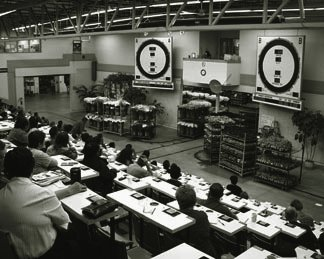
\includegraphics[width=\marginparwidth]{auctions/flowermarket}
  Ontario Flower Growers Co-op, an example of a Dutch auction at work.
  The two large circles in the back are used to show the descending
  price.}

The \td{Dutch} auction is an \td{open-cry descending price} auction.
In it the seller continuously lowers the selling price until a buyer
hits a buzzer, agreeing to buy at the current price. The auction's
name comes from its use by the Dutch to sell flowers. The Dutch flower
markets have been around for centuries and are still thriving. Every
morning carts of flowers are paraded before eager flower shop owners
who are equipped with a buzzer. Each cart stops before the buyers and
a clock starts ticking backwards from a high number. When the first
buyer hits his buzzer the flowers are sold to him at the current
price. Analysis of the Dutch auction shows that it is equivalent to a
first-price sealed-bid auction in terms of strategy. That is, it has
no dominant strategy. However, it has the nice property of being
real-time efficient. The auction closes quickly and the auctioneer can
make it move even faster by lowering the price faster.  This real-time
efficiency makes it a very attractive auction for selling cut flowers
as these lose their value quickly after being harvested.

\medskip

%\begin{figure}
%  \begin{center}
%    \includegraphics[width=.4\textwidth]{google}
%  \end{center}  
%  \caption{A visual explanation of the Google IPO auction, from the New York Times.}
%  \label{fig:google}
%\end{figure}

%A few years ago Google utilized a variation on the Dutch auction to
%determine the initial price for their shares. They asked all buyers to
%submit their bids. Each bid contained the number of shares and the
%price per share the buyer was willing to pay. They then sorted all
%these and, starting from the highest bids, counted backwards until
%they had sold all their shares. The price that they sold at was given
%by the last price price they counted (that is, the smallest price).
%The method is nicely summarized by the graph shown in
%Figure~\ref{fig:google}. It seems to me, however, that the Google
%auction was more similar to a Vickrey auction than to a Dutch auction.
%I don't understand why they called it a Dutch auction. 

The \td{Vickrey} auction is a more recent addition and has some very
interesting properties. It is a \td{second-price sealed-bid} auction.
All agents place their bids and the agent with the highest bid wins
the auction but the price he pays is the price of the second highest
bid. Analysis of this auction has shown that bidding one's true
valuation, in a private value auction, is the dominant strategy. For
example, let your valuation for the item being sold be $v$.  If you
bid less than $v$ then you are risking the possibility that some other
agent will bid $w < v$ and get the item even though you could have won
it.  Moreover, since $w$ is less than $v$ you could have bid $v$ and
paid only $w$.  As such, you have nothing to gain by bidding less than
$v$ but risk the possibility of losing an auction that you could have
won at an acceptable price. On the other hand, if you bid $v' > v$
then you are risking that some other agent will bid $w$, where $v'> w
> v$, and thereby cause you to pay more than your reservation price
$v$. At the same time, you do not gain anything by bidding higher than
$v$ because the only auction that you might win by bidding $v'$
instead of $v$ are those where you have to pay more than $v$.

\mpic{auctions/vickrey}{William Vickrey}{1914}{1996}{Nobel Prize in
  Economics.} As such, the Vickrey auction eliminates the need for
strategizing.  Since there is an easy dominant strategy the agents do
not have to think about what they should do. They just play their
dominant strategy and bid their true valuation. Thus makes it a very
attractive auction in terms of its efficiency but it is also for this
reason that most people don't like Vickrey auctions. People are often
hesitant about revealing their true valuations for an item because we
know that the world is an iterated game and this information could be
used against us in some future auction. As such, Vickrey auctions are
seldom used in the real world.  \medskip

Finally, the \td{double auction} is a way of selling multiple units of
the same item. It is the auction used in stock markets. Each buyer
places either a buy or a sell order at a particular price for a number
of instances of the item (number of shares in the stock-market). The
buy and sell bids can be visualized in a simple graph such as the one
shown in Figure~\ref{fig:double}. Here, the $x$-axis represents a
price and each box represents an offer to buy or sell a share at the
given price.

\begin{SCfigure}
  \begin{minipage}{1.0\linewidth}
    \begin{center}
      \begin{tikzpicture}[style=dstyle,minimum size=.8cm]
        \draw[|->] (.4,0) -- (6.1,0);

        \node at (1,-2.5)[color=gray] {\textcolor{black}{1}};
        \node at (2,-2.5)[color=gray] {\textcolor{black}{2}};
        \node at (3,-2.5)[color=gray] {\textcolor{black}{3}};
        \node at (4,-2.5)[color=gray] {\textcolor{black}{4}};
        \node at (5,-2.5)[color=gray] {\textcolor{black}{5}};
        
        \node (s1) at (1,.5)[draw] {Sell};
        \node (s2) at (1,1.5)[draw] {Sell};
        \node (s3) at (2,.5)[draw] {Sell};
        \node (s4) at (3,.5)[draw] {Sell};
        \node (s5) at (5,.5)[draw] {Sell};

        \node (b1) at (1,-.5)[draw,color=gray] {\textcolor{black}{Buy}};
        \node (b2) at (2,-.5)[draw,color=gray] {\textcolor{black}{Buy}};
        \node (b3) at (2,-1.5)[draw,color=gray] {\textcolor{black}{Buy}};
        \node (b4) at (3,-.5)[draw,color=gray] {\textcolor{black}{Buy}};
        \node (b5) at (4,-.5)[draw,color=gray] {\textcolor{black}{Buy}};

        % \only<2>{
        %   \draw (s1) -- (b1);
        %   \draw (s2) -- (b2);
        %   \draw (s3) -- (b3);
        %   \draw (s4) -- (b4);}

        % \only<3>{
        %   \draw (s1) -- (b5);
        %   \draw (s2) -- (b4);
        %   \draw (s3) -- (b3);}
        
      \end{tikzpicture}
    \end{center}
  \end{minipage}
  \caption{Graphical representation of a double auction. The
    $x$-axis represents prices. Each box represents one buy or sell
    order at the given price.}
  \label{fig:double}
\end{SCfigure}

Once we have all the bids then it is time to clear the auction.  There
are many different ways to clear a double auction. For example, if
figure~\ref{fig:double} we could match the sell order for 1 with the
buy for 5 then pocket the difference of $5 - 1 = 4$ for ourselves, or
we could clear it at 3 and thus give both bidders a deal, or we could
match the seller for 1 with the buy for 1, and so on. As can be seen,
there are many different ways to match up these pairs and it is not
clear which one is better.

One metric we might wish to maximize is the amount of surplus, known
as the spread by traders. That is, the sum of the differences between
the buy bids and the sell bids. In some auctions this surplus is kept
by the auctioneer who then has an incentive to maximize it. Another
option is to use it to enable more bids to clear.  In the example
above the total supply and demands are 12, therefore all bids should
clear. One way to do this is to pair up all the small sell bids and
give these sellers exactly what they asked for then give the surplus
to the sell bid of 5 in order to clear it with the remaining buy bid.

Another metric we could use is a uniform price. That is, rather than
giving each seller and buyer the exact price they asked for, we give
them all one uniform clearing price. Clearly, the only buy bids that
will clear are those that are above the clearing price and the only
sell bids that clear are those below the clearing price.

\subsection{Analysis}

Now that we know the various auction types, there is an obvious
question that we must ask ourselves. On which auction do sellers make
more money? This question is answered by the following theorem.

\begin{theorem}[Revenue Equivalence]
  \label{th:revenue-eq}
  All four single-item auctions produce the same expected revenue in
  private value auctions with bidders that are risk-neutral.
\end{theorem}

We also know that if the bidders are risk-averse then the Dutch and
first-price are better.  A risk-averse bidder is willing to pay a bit
more than their private valuation in order to get the item. In a Dutch
or First-price auction a risk-averse agent can insure himself by
bidding more than would be required.

In common or correlated value cases the English auction gives a higher
revenue to the seller.  The increasing price causes others to increase
valuation.  That is, once the agent sees others bidding very high for
the item the agent realizes that the item is really worth more to the
other agents so it also raises its valuation of the item.\footnote{An
  interesting example of this was a British auction for 3G bandwidth
  licenses. The standard English auction was modified so that everyone
  must agree to buy at the current price or leave the room. This led
  to the licenses selling for 1000 times the expected amount
  \cite{harford05a}.}
\medskip

As it is often the case when money is involved, we have to be on the
look out for ways in which the agents might cheat. The problem of
\td{bidder collusion} affects all 4 auctions. In bidder collusion the
bidders come to an a-priory agreement about what they will bid.  They
determine which one of them has the higher valuation and then all the
other bidders refrain from bidding their true valuation so that the
one agent can get it for a much lower price. The winner will then need
to payback the others. The English and Vickrey auctions are especially
vulnerable to bidder collusion as they \td{self-enforce collusion}
agreements. For example, say there are 10 buyers and they realize that
one of them has a valuation of 100 while the others have a valuation
of 50 for the item. They agree to let him buy it for 1. In an English
auction one of the 99 agents could defect and bid 2. However, this
would only make the high-valuation agent bid 3, and so on until they
get to 51. The high-valuation agent will get the item for 51 so the
other agent gets nothing by defecting. The same logic applies in a
Vickrey auction.

Another problem might be that a \td{lying auctioneer} can make money
from a Vickrey auction. All he has to do is to report a higher
second-price than the one that was announced. The winner then pays
this higher second price to the auctioneer who gives the buyer the
real second price and pockets the difference. This requires that the
bids are not revealed and that the buyer does not pay the seller
directly. If the buyer paid the seller directly then a lying
auctioneer and the seller could collude to charge the buyer a higher
price. A lying auctioneer can also place a \mc{\textbf{shill}: a decoy
  who acts as an enthusiastic customer in order to stimulate the
  participation of others.} shill in an English auction. That is,
assuming that the auctioneer gets paid a percentage of the sales
price. If the auctioneer gets paid a fixed amount then there is no
incentive for him to increase the sales price.
\medskip 

When auctioning items in a series when their valuations are
interrelated, such as chairs in a dining set or bandwidth rights in
adjacent counties, it is possible to arrive at inefficient
allocations. For example, the problem in Table~\ref{tab:inef} leads to
an inefficient allocation if we first auction $t_1$ and then $t_2$.
Specifically, if we auction $t_1$ first then Agent 2 will get it as it
has the lower cost. When we then auction $t_2$ both agents have the
same cost (1) but, no matter who gets it the total cost is 2.5. If, on
the other hand agent 1 had won both tasks then the total cost would be
2.  matter who gets it the total cost is 2.5. This is the problem of
\td{inefficient allocation}.

\begin{SCtable}
  \begin{minipage}{1.0\linewidth}
    \begin{center}
      Costs of Doing Tasks
      \begin{tabular}{ccc}\toprule
        tasks&Agent 1&Agent 2\\ \midrule
        $t_1$&2&1.5\\ 
        $t_2$&1&1.5\\ 
        $t_1$,$t_2$&2&2.5\\ \bottomrule
      \end{tabular}
    \end{center}
  \end{minipage}
  \caption{Example of inefficient allocation.}
  \label{tab:inef}
\end{SCtable}

We could solve this problem if we made the agents use full lookahead
effectively building an extended-form game from their possible
interactions. With full lookahead the agents can build a tree where
each level corresponds to a task being auctioned.  In this way agent 1
can see that it will only cost him 2 to do $t_1$ and $t_2$ so it can
reduce its cost for $t_1$ from 2 to 1. Of course, this puts agent 1 at
risk of not getting $t_2$ since agent 1 generally will not know agent
2's cost for t2 so it does not know if it will win that auction.
Another much better way of solving the problem of inefficient
allocations is to use a combinatorial auction, which we will learn
about in Section~\ref{sec:ca}.

\subsection{Auction Design}

When designing an auction for a multiagent system you must make many
decisions. You must first determine what kind of control you have over
the system. It is possible that you control only the bidding agent and
the auction is already implemented, as when building agents to bid on
Ebay. It is possible that you control only the auction mechanism, as
when building an auction website. Finally, it is possible that you
might control both agents and mechanism, as when building a closed
multiagent system.

The case where you control the mechanism is especially interesting.
You must then decide what bidding rules you will use: when bids are to
be placed, when they can no longer be placed, what form can these bids
takes, and what rules they must follow. For example, you might set a
rule that a new bid has to always be for a higher value. You also set
up clearing rules which determine when the items are sold. We
explained some of the problems with various clearing rules in the
double auction. The four standard auction types already have clearing
rules but you might want to modify these. Finally, you must decide on
information rules: how much information the agents are to know about
what the other agents bid, whether to reveal information during the
bidding process itself or after clearing \cite{wurman02a}.

Currently all online auctions are implemented as centralized web
applications but it is not hard to imagine a future where the auctions
are freed from the constraints of a central hub and become a protocol
enacted by buying and selling agents.

\section{Combinatorial Auctions}
\label{sec:ca}

Arguably, the \td{combinatorial auction} has been the most widely used
auction in multiagent systems. In it agents can place bids for sets of
items instead of just placing one bid for each item for sale. In many
systems we have the problem that there is a set of tasks or jobs that
needs to be distributed among the agents but the agents have complex
preferences over the set of tasks. For example, in a workflow
application we have a set of workflows, each composed of a set of web
services, which must be performed by certain deadlines.  Each agent
can perform a subset of the services but each agent has different
costs which might depend on the agent's type, its current load, the
services it has done before, etc. Our problem as system designers is
to allocate the workflows to agents so that we maximize the total
number of workflows completed. Another example of combinatorial
auctions is the selling of broadcasting rights by the federal
government where cellular companies prefer to own the same frequencies
in nearby locations, or at least to own some bandwidth in all the
neighborhoods of a city. A final example is the buying of parts to put
together a PC which requires a motherboard, CPU, ram, etc.  Each part
can be bought independently but only some bundles work together.
These problems, and all problems of this type, can be solved by a
combinatorial auction.

Formally, we define a combinatorial auction over a set of items $M$ as
being composed of a set of bids, where each agent can supply many
different bids for different subset of items. Each bid $b \in B$ is
composed of \bidi{}, which is the set of items the bid is over,
\bidv{} the value or price of the bid, and \bida{} which is the agent
that placed the bid.

\pgfdeclareimage[interpolate=true,width=6cm]{titans}{auctions/teentitansf}

\begin{SCfigure}
  \begin{minipage}{1.0\linewidth}
    \begin{center}
      \begin{tikzpicture}[style=dstyle]
        \pgftext[at=\pgfpoint{-3cm}{0cm}]{\pgfuseimage{titans}};
        \node at (3,0) {
          \begin{tabular}{lc}\toprule
            Price &Bid items  \\ \midrule
            \$$1$  &Beast Boy \\ 
            \$$3$  &Robin \\ 
            \$$5$  &Raven, Starfire \\ 
            \$$6$  &Cyborg, Robin \\ 
            \$$7$  &Cyborg, Beast Boy \\ 
            \$$8$  &Raven, Beast Boy \\ \bottomrule
          \end{tabular}};
      \end{tikzpicture}
    \end{center}
  \end{minipage}
  \caption{Teen Titans figurines: (from top left) Beast
    Boy, Cyborg, Robin, Raven, and Starfire. The set of
    combinatorial bids received for them in on the table at the
    right.}
  \label{fig:titans}
\end{SCfigure}

For example, say you had a set of 5 figurines, one each of a different
Teen Titan and you received 6 different combinatorial bids, as shown
in Figure~\ref{fig:titans}.  The question you then face is how to
determine which are the winning bids so as to maximize the amount of
revenue you receive. Note that you can sell each item only once since
you only have one of each. This is the problem of winner
determination. In the figure, the correct solution would be to accept
the \$3, the \$5 and the \$7 bids.


\subsection{Centralized Winner Determination}

The \td{winner determination} problem is finding the set of bids that
maximizes the seller's revenue. Or, more formally, find

\begin{equation}
  \label{eq:wdp}
  X^* = \arg \max_{X \subseteq C} \sum_{b \in X} \bidv{}
\end{equation}
where $C$ is a set of all bid sets in which none of the bids share an
item, that is
\begin{equation}
  \label{eq:complete}
  C = \{Y \subseteq B \,|\, \forall_{a,b' \in Y} a^{\text{items}} \cap \bidi = \emptyset\}.
\end{equation}

\mc{A variation on this problem is when agents can submit \acro{xor}
  bids.  That is, when an agent can say that it wants only one of his
  bids to win. Computationally, both problems are similar.}

Unfortunately, this is not a simple problem as there are, in the worst
case, many possible bidsets. Specifically, if bids exists for all
subsets of items then $X$ is a way of partitioning the set of items
$S$ into non-overlapping subset. That is, take the set of items $S$
and figure out how many ways it can be split into smaller sets. We can
calculate this number by remembering that the \td{Stirling number of
  the second kind} gives us the number of ways to partition a set of
$n$ elements into $k$ non-empty sets. Namely,
\begin{equation}
  \label{eq:stirling}
  S(n,k) = \frac{1}{k!} \sum_{i=0}^{k-1} (-1)^i \binom{k}{i}(k-i)^n.
\end{equation}

Using this formula we can easily determine that the total number of
allocations of $m$ items is given by
\begin{equation}
  \label{eq:num-allocations}
\sum_{i=1}^{m} S(m,i),
\end{equation}
which is bounded by
\[O(m^m) \mbox{ and } \omega(m^{m/2}).\]

This means that a brute force search of all possible allocations of
items to agents is computationally intractable. In fact, no approach
will work in polynomial time.

\begin{theorem} Winner Determination in Combinatorial Auction is
  NP-hard. That is, finding the $X^*$ that satisfies \eqref{eq:wdp} is
  NP-hard \cite{rothkopf98a}.
\end{theorem}

Even simplifying the problem does not make it easier to solve. For
example, say that instead of trying to find the best allocation we
simply want to check if there exists an allocation with total revenue
of at least $w$. We call this the \td{decision version} of the winner
determination problem. Lets also further restrict the types of bids
the agents can submit. Even under these circumstances the problem
remains hard.

\begin{theorem}
  The decision version of the winner determination problem in
  combinatorial auctions is NP-complete, even if we restrict it to
  instances where every bid has a value equal to 1, every bidder
  submits only one bid, and every item is contained in exactly two
  bids \cite[Chapter 12]{cramton06a}.
\end{theorem}

Thus, the problem is very hard, even when we try to limit its
complexity. But, there is some hope. The winner determination problem
in combinatorial auctions can be reduced to a \td{linear programming}
problem and, therefore, solved in polynomial time with well-known
algorithms but only if prices can be attached to single items in the
auction \cite{nisan00a}. That is, there needs to be a singleton bid
for every item. In many cases we can satisfy this requirement by
simply adding the missing singleton bids, each with a value of 0.
Specifically, the linear program which models the winner determination
problem is to find the $x$ that satisfies the following:

\mc{Simplex is the most widely used linear programming algorithm.  It
  has worst-case exponential time, but in practice it is much faster.
  Other algorithms exist that are guaranteed polynomial.}
\textbf{Maximize:}
\[\sum_{b \in B} x[b] \bidv\]

\textbf{Subject to:}
\[\sum_{b \,|\, j \in \bidi} x[b] \leq 1, \forall j \in M\]
\[x[b] \in \{0,1\}, \forall b \in B,\]

where $x[b]$ is a bit which denotes whether bid $b$ is a winning bid.
That is, maximize the sum of the bid values given that each item can
be in, at most, one winning bid.  It has also been shown that the
linear programming problem will solve a combinatorial auction when the
bids satisfy any one of the following criteria \cite{nisan00a}:
\begin{enumerate}
\item All bids are for consecutive sub-ranges of the items.
\item The bids are hierarchical.
\item The bids are only \acro{or}-of-\acro{xor}s of singleton bids.
\item The bids are all singleton bids.
\item The bids are downward sloping symmetric.
\end{enumerate}

\medskip

A different approach to solving the winner determination problem is to
conduct one of the standard \acro{ai}-searches over all possible
allocations, given the bids submitted. The advantage over using a
linear programming solver is that we can tweak our \acro{ai} search
algorithms and optimize them to solve our specific problem. That is,
we can put some of our domain knowledge into the algorithm to make it
run faster, as we shall see.


\begin{SCfigure}
  \begin{minipage}{1.0\linewidth}
    \begin{codebox}
      \Procname{$\proc{build-branch-on-items-search-tree}$}
      \li Create a singleton bid for any item that does not have one
      \li Number items from 1 to $m$
      \li Create empty root node
      \li \For $n \in M$ in order
      \li \Do Add as its children all bids that 
      \li \> include the smallest item that is not an ancestor of $n$ but
      \li \> that do not include any item that is an ancestor of $n$.
      \End
    \end{codebox}    
  \end{minipage}
  \caption{Algorithm for building a branch on items search tree. This
    algorithms does not find a solution, it only builds a tree for the
    purpose of illustration.}
  \label{fig:bob-tree}
\end{SCfigure}

\begin{SCfigure}
  \begin{minipage}{1.0\linewidth}
  \begin{center}
    \begin{tikzpicture}[style=dstyle]
      \tikzstyle{every node}=[draw]
\node[fill,circle] {} [sibling distance=2.2cm,level distance=1cm]
child {node {12} [sibling distance=1cm]
         child {node {35}
                   child {node {4}}}
         child {node {3}
                   child {node {4}
                            child {node {5}}}}}
child {node {135}
          child {node {2}
                   child {node {4}}}}
child {node {14} [sibling distance=1.2cm]
          child {node {25}
                   child {node {3}}}
          child {node {2} [sibling distance=.8cm]
                   child {node {35}}
                   child {node {3}
                            child {node {5}}}
                 }}
child {node {1} [sibling distance=1.2cm]
          child {node {25}
                    child {node {3}
                             child {node {4}}}}
          child {node {2} [sibling distance=.8cm]
                    child {node {35}
                             child {node {4}}}
                    child {node {3}
                             child {node {4}
                                      child {node {5}}}}
                  }};
\node at (-5,0) {1};
\node at (-5,-.5) {2};
\node at (-5,-1) {3};
\node at (-5,-1.5) {4};
\node at (-5,-2) {5};
\node at (-5,-2.5) {12};
\node at (-5,-3) {135};
\node at (-5,-3.5) {14};
\node at (-5,-4) {25};
\node at (-5,-4.5) {35};
    \end{tikzpicture}
  \end{center}
  \end{minipage}
  \caption{Branch on items search tree for winner determination in
    combinatorial auctions. Note that this tree has 9 leafs (9
    possible ways of selling all items given the bids) while the total
    number of dividing 5 items into subsets is 52.}
  \label{fig:tree}
\end{SCfigure}

Before we can do search we need to define our search tree. One way we
can build a search tree is by having each node be a bid and each path
from the root to a leaf correspond to a set of bids where no two bids
share an item. The algorithm for building this tree is shown in
figure~\ref{fig:bob-tree}. We refer to this tree as a \td{branch on
  items} search tree. Figure~\ref{fig:tree} shows an example tree
built in this fashion. In this case we have five items for sale,
numbered 1--5.  The column on the left lists all the bids received. We
omit the bid amount and only show the set of items for each bid. The
search algorithm uses these bids to build the tree shown on the right
of the figure.  We start at the first level from the top.  All the
children of the root are bids that have item 1 in them. Then, we
proceed to add children to each node.  The children of every node will
be all the bids that contain the smallest number that is \textbf{not}
on the path from the root to the node. Since the algorithm has the
provision of adding a singleton bid with value 0 for every item, we
are guaranteed to find a suitable bid as a children of every node. The
only time we cannot find such a bid is when the path from the root to
the node contains all items. In this case the node is a leaf and the
set of bids from root to leaf constitutes a possible bid set.

The speedup of this search over the brute force method of considering
all possible ways of breaking up 5 items into subsets can be confirmed
by the fact that this tree has 9 leafs, therefore only 9 working bid
sets exists. Meanwhile, the application of the Stirling formula gives
us

\[\sum_{i = 1\ldots5} S(5,i) = 52,\]

which means that there are 52 ways to break up 5 items into subsets.
Clearly, fewer bids means faster run time which is the central idea of
the search algorithm. In general, we know that the number of leafs in the
tree is bounded.
\begin{theorem}
  The number of leaves in the tree produced by
  \proc{build-branch-on-items-search-tree} is no greater than
  $(|B|/|M|)^{|M|}$. The number of nodes is no greater than $|M|$
  times the number of leaves plus 1 \cite{sandholm02b}.
\end{theorem}

We can also build a binary tree where each node is a bid and reach
edge represents whether or not that particular bid is in the solution.
We refer to this tree as a \td{branch on bids} search tree, an example
is shown in Figure~\ref{fig:branchonbids}. Each edge on the tree
indicates whether the parent node (bid) is to be considered as part of
the final bidset. For example, the rightmost branch of the tree
consists of all ``In'' branches so the rightmost leaf node corresponds
to the bidset $(35)(14)(2)$ which forms a complete allocation. In
practice, the branch on bids search tree is often faster than the
previous tree because it gives us more control over the order of bids
so we can better optimize the bid order. Also, the branch on bids
search does not require us to add dummy singleton bids.


\begin{SCfigure}
  \begin{minipage}{1.0\linewidth}
    \begin{center}
    \begin{tikzpicture}[style=dstyle]
\node[draw] {35} [sibling distance=4cm,level distance=1.2cm]
child {node[draw] {25} [sibling distance=2cm]
  child {node[draw] {14} [sibling distance=1cm]
    child {node[draw] {135} [sibling distance=.5cm]
      child[->] {node {}}
      child[->] {node {}}
      edge from parent node[left,near start] {Out}}
    child {node[draw] {5} [sibling distance=.5cm]
      child[->] {node {}}
      child[->] {node {}}
      edge from parent node[right,near start] {In}}
    edge from parent node[left,near start] {Out}}
  child {node[draw] {14} [sibling distance=1cm]
    child {node[draw] {5} [sibling distance=.5cm]
      child[->] {node {}}
      child[->] {node {}}
      edge from parent node[left,near start] {Out}}
    child {node[draw] {3} [sibling distance=.5cm]
      child {node[draw,fill] {}}
      child {node[draw,fill] {}}
      edge from parent node[right,near start] {In}}
    edge from parent node[right,near start] {In}}
  edge from parent node[left,near start] {Out}
}
child {node[draw] {14} [sibling distance=2cm]
  child {node[draw] {12} [sibling distance=1cm]
    child {node[draw] {4} [sibling distance=.5cm]
      child[->] {node {}}
      child[->] {node {}}
      edge from parent node[left,near start] {Out}}
    child {node[draw] {4} [sibling distance=.5cm]
      child {node[draw,fill] {}}
      child {node[draw,fill] {}}
      edge from parent node[right,near start] {In}}
    edge from parent node[left,near start] {Out}}
  child {node[draw] {2}  [sibling distance=1cm]
    child {node[draw,fill] {} edge from parent node[left,near start] {Out}}
    child {node[draw,fill] {} edge from parent node[right,near start] {In}}
    edge from parent node[right,near start] {In}}
  edge from parent node[right,near start] {In}};
\node[draw] at (-5,0) {1};
\node[draw] at (-5,-.5) {2};
\node[draw] at (-5,-1) {3};
\node[draw] at (-5,-1.5) {4};
\node[draw] at (-5,-2) {5};
\node[draw] at (-5,-2.5) {12};
\node[draw] at (-5,-3) {135};
\node[draw] at (-5,-3.5) {14};
\node[draw] at (-5,-4) {25};
\node[draw] at (-5,-4.5) {35};
    \end{tikzpicture}
    \end{center}
  \end{minipage}
  \caption{Branch on bids partial tree. The black boxes indicate
    search paths that have terminated because they denote a complete
    set of bids, that is, no more bids can be added because they
    contain items already sold.}
  \label{fig:branchonbids}
\end{SCfigure}

We now have to decide how to search our chosen tree. Since both trees
have a number of nodes that is exponential on the number of bids a
breadth first search would require too much memory. However, a depth
first search should be possible, but time consuming. A branch and
bound algorithm like the one we used for \acro{dcop} in
Chapter~\ref{sec:dcop} further helps reduce the search space and speed
up computation.  In order to implement it we first need a function $h$
which gives us an upper bound on the value of allocating all the items
that have yet to be allocated. One such function is $h$
\begin{equation}
  \label{eq:ca-heuristic}
  h(g) = \sum_{j \in M - \bigcup_{b \in g} \bidi} \max_{b | j \in \bidi}
  \frac{\bidv}{|\bidi|},
\end{equation}
where $g$ is the set of bids that have been cleared. The function $h$
simply adds up the maximum possible revenue that each item not in $g$
could contribute by using the bid that pays the most for each item,
divided by the number of items on the bid.  This function provides an
upper bound since no feasible bidset with higher revenue can exist.

\begin{SCfigure}
  \begin{minipage}{1.0\linewidth}
    \begin{codebox}
      \Procname{$\proc{branch-on-bids-ca}()$}
      \li $r* \gets 0$ \>\>\>\Comment Max revenue found. Global variable.
      \li $g* \gets \emptyset$ \>\>\>\Comment Best solution found. Global
      variable.
      \li $\proc{branch-on-bids-ca-helper}(\emptyset,B)$
      \li \Return $g^*$
    \end{codebox}
    \begin{codebox}
    \Procname{$\proc{branch-on-bids-ca-helper}(g,\id{available-bids})$}
    \li \If $\id{available-bids} = \emptyset$
    \li \Then \Return
        \End
    \li \If $\bigcup_{b \in g} \bidi = M$   \>\>\>\>\>\>\>\>\>\>\> \Comment $g$
    covers all items
    \li \Then \If $\sum_{b \in g} \bidv > r^*$ \>\>\>\>\>\>\>\>\>
    \Comment $g$ has higher revenue than $r^*$
    \li       \Then $g^* \gets g$
    \li             $r^* \gets \sum_{b \in g} \bidv$
              \End
    \li       \Return
        \End
    \li $\id{next} \gets \proc{first}(\id{available-bids})$
    \li \If $\id{next}^{\text{items}} \cap \bigcup_{\bidp \in g}
    \bidpi = \emptyset\} $ \>\>\>\>\>\>\>\>\>\>\> \Comment \id{next}'s
    items do not overlap $g$
    \li \Then $g' \gets g + \id{next}$
    \li     \If  $\sum_{\bidp \in g'} \bidpv + h(g') > r^*$
    \li     \Then \proc{branch-on-bids-ca-helper}$(g',\proc{rest}(\id{available-bids}))$
            \End
         \End
    \li \proc{branch-on-bids-ca-helper}$(g,\proc{rest}(\id{available-bids}))$
    
%     \li \For $b \in \{b \in B \,|\, \bidi \cap \bigcup_{\bidp \in g}
%     \bidpi = \emptyset\} $ \>\>\>\>\>\>\>\>\>\>\> \Comment $b$'s items do not
%     overlap $g$
%     \li \Do $g' \gets g + b$
%     \li     \If $\sum_{\bidp \in g'} \bidpv + h(g') > r^*$
%     \li     \Then \proc{branch-on-bids-ca-helper}$(g')$
%             \End
%         \End
  \end{codebox}
  \end{minipage}
  \caption{A centralized branch and bound algorithm that searchers a
    branch on bids tree and finds the revenue maximizing solution
    given a set $B$ of combinatorial bids over items $M$.}
  \label{fig:bb-ca}
\end{SCfigure}

Given the upper bound $h(g)$ we can then implement the branch and
bound algorithm shown in figure~\ref{fig:bb-ca}. This algorithm
searches the branch on bids tree. It maintains a partial solution $g$
to which it adds one bid on each recursive call.  Whenever it realizes
that partial solution will never be able to achieve revenue that
is higher than the best revenue it has already found then it gives up
on that subtree, see line~8 of \proc{branch-on-bids-ca-helper}. This
algorithm is complete and thus guaranteed to find the revenue
maximizing bidset.

We can also use the same heuristic function to do an \astar{} search.
Unfortunately, since \astar{} acts much like a breadth first search it
generally consumes too much memory. A viable solution is to use
iterative deepening \astar{}. \idastar{} guesses how much revenue we
can expect and runs a depth-first search that prunes nodes that have
used more than that. If a solution is not found then the guess is
reduced and we try again. \idastar{}, with some optimizations, was
implemented by the \td{Bidtree} algorithm \cite{sandholm99a} on the
branch on items search tree. In practice, this approach was found to
often be slower than a branch and bound search.


The \proc{branch-on-bids-ca} algorithm is the basic framework for the
Combinatorial Auction Branch on Bids (\td{CABOB}) algorithm
\cite{sandholm05a}.  \acro{cabob} improves the performance of the
basic algorithm in several ways, one of which is by improving the
search for new bids to add to the partial solution. Specifically, we
note that a naive implementation of line~6 of
\proc{branch-on-bids-ca-helper} would mean that we would build this
set on each recursive call to the function.  That would be very time
consuming as there are an exponential number of bids in $B$.
\acro{cabob} handles this problem by maintaining graph data structure
which has all the bids that can still be used given $g$. The nodes in
the graph are the bids that are still available and the edges connect
every pair of bids that share an item.  In this way when a new bid is
added to $g$ it is removed from the graph as well as all the other
bids that are connected to it.


\begin{SCfigure}
  \begin{minipage}{1.0\linewidth}
    \begin{codebox}
      \Procname{$\proc{branch-on-items-ca}()$}
      \li $r* \gets 0$ \>\>\>\Comment Max revenue found. Global variable.
      \li $g* \gets \emptyset$ \>\>\>\Comment Best solution found. Global
      variable.
      \li $\proc{branch-on-items-ca-helper}(1,\emptyset)$
      \li \Return $g^*$
    \end{codebox}
    \begin{codebox}
    \Procname{$\proc{branch-on-items-ca-helper}(i,g)$}
    \li \If $i = m$   \>\>\>\>\>\>\>\>\>\>\> \Comment $g$
    covers all items
    \li \Then \If $\sum_{b \in g} \bidv > r^*$ \>\>\>\>\>\>\>\>\>
    \Comment $g$ has higher revenue than $r^*$
    \li       \Then $g^* \gets g$
    \li             $r^* \gets \sum_{b \in g} \bidv$
              \End
    \li       \Return
        \End              
    \li \For $b \in \{b \in B \,|\, i \in \bidi \wedge \bidi \cap \bigcup_{\bidp \in g}
    \bidpi = \emptyset\} $ \Comment $b$'s items do not overlap $g$ 
    \li \Do $g' \gets g + b$
    \li     \If $\sum_{\bidp \in g'} \bidpv + h(g') > r^*$
    \li     \Then \proc{branch-on-items-ca-helper}$(i+1, g')$
            \End
        \End
  \end{codebox}
  \end{minipage}
  \caption{A centralized branch and bound algorithm that searchers a
    branch on items tree and finds the revenue maximizing solution
    given a set $B$ of combinatorial bids over items $M$.}
  \label{fig:bb-boi-ca}
\end{SCfigure}


\netlogo{ca}We can also perform the branch and bound search on the
branch on items search tree, as shown in Figure~\ref{fig:bb-boi-ca}.
This algorithm is the basis for the \td{CASS} (Combinatorial Auction
Structured Search) algorithm which also implements further refinements
on the basic algorithm \cite{fujishima99a}.

Most algorithms for centralized winner determination in combinatorial
auction expand on the basic branch and bound search by using
specialized data structures to speed up access to the information
need---the viable bids given the current partial solution---and
implement heuristics which have been shown to reduce the size of the
search space, especially for certain popular bid distributions.  Some
heuristics that have been found useful include the following:

\begin{itemize}
\item Keep only the highest bid for any set. That is, if there is a
  bid of \$10 for items 1,2 and another bid of \$20 for 1,2 then we
  get rid of the \$10 bid.

\item Remove provably noncompetitive bids, that is, those that are
  dominated by another bid or sets of bids. For example, if there is
  a bid for \$10 for item 1 and another bid for \$5 for items 1,2 then
  the \$10 bid dominates the \$5 bid---any situation in which we
  choose the \$5 bid would be made better if we changed that bid for
  the \$10 bid.

\item Decompose bids into connected sets, each solved independently.
  If we can separate the set of bids into two or more sets of bids
  where all bids for any item are to be found in only one of the sets
  then this set of bids becomes a smaller, and independent, winner
  determination problem.
    
\item Mark noncompetitive tuple of bids. For example, if there are
  bids \$1:(1,2), \$1:(3,4), \$10:(1,3), \$10:(2,4) then the pair of
  \$10 bids dominates the pair of \$1 bids, so we can get rid of them.

\item In the branch-on-items tree place the items with the most bids
  first on the tree. This way the most constrained items are tried
  first thereby creating fewer leafs.

\item If the remaining search subtree is the same for different nodes in
  the search tree, as can happen when different items are cleared but
  by different bids, then these subtrees can be cached. The subtree is
  solved once and the answer, that is, the best set of bids found in
  it, is saved for possible future use.

\end{itemize}

In general the best speed attainable by the best algorithms varies
greatly depending on the type of bids submitted. For example, if the
number of items in each bid is chosen from a flat probability
distribution then we can solve problems with thousands of items and
tens of thousands of bids in seconds. On the other hand, if each bid
contains exactly five randomly chosen items and a price of 1 then we
can only solve problems with tens of items and hundreds of bids in a
minute. The Combinatorial Auction Test Suite (\td{CATS}) can generate
realistic types of bid distributions so new algorithms can be compared
to existing ones using realistic bid sets \cite{leyton-brown00a}. It
generates these bids by using several sample scenarios. In one
scenario there is a graph where the nodes represent cities and the
edges are railroad tracks that connect these cities. The items for
sale are the tracks between cities, that is, the edges. The agents are
given pairs of host/destination cities and are told that they need to
establish a train route between their city pairs. Thus, each agent
determines all the possible sets of edges which connect his city pairs
and submits \acro{xor} combinatorial bids on them. The value of each
path depends on the total distance; shorter routes are preferred.


\subsection{Distributed Winner Determination}

One problem with the centralized winner determination algorithms,
aside from the bottleneck, is that they require the use of a trusted
auctioneer who will perform the needed computations. Another option is
to build a peer-to-peer combinatorial auction protocol which lets the
sellers themselves determine the winning set of bids and discourages
them from cheating.

\subsubsection{Incremental Auctions: Distribute over Bidders}
\label{sec:incremental-auctions}

One way to distribute the winner determination calculation is by
offloading it on the bidding agents. We can do this by using an
increasing price auction and making the bidders figure out which bids
would be better than the current standing bid. This is the approach
taken by the Progressive Adaptive User Selection Environment or
\td{PAUSE} combinatorial auction \cite{kelly00a} \cite[Chapter
6]{cramton06a}.

A \acro{pause} auction for $m$ items has $m$ stages. Stage 1 consists
of having simultaneous ascending price open-cry auctions for each
individual item. During this stage the bidders can only place
individual bids on items. At the end of this state we will know what
is the highest bid for each individual item and who placed that bid.
In each successive stage $k=2,3,\ldots,m$ we hold an ascending price
auction where the bidders must submit sets of bids that cover all
items but each one of the bids must be for $k$ items or less.  The
bidders are allowed to use bids that other agents have placed in
previous rounds. Also, any new bid set has to have a sum of bid prices
which is bigger than the currently winning bid set.

At the end of each stage $k$ all agents know the best bid for every
subset of size $k$ or less. Also, at any point in time after stage 1
has ended there is a standing bid set whose value increases
monotonically as new bid sets are submitted. Since in the final round
all agents consider all possible bid sets, we know that the final
winning bid set will be one such that no agent can propose a better
bidset. Note, however, that this bid set will generally not be $X^*$
since we are using ascending price auction so the winning bid will be
only slightly bigger than the second highest bid for the particular
set of items.

In the general case, the \acro{pause} auction has been shown to be
\td{envy-free} in that at the conclusion of the auction no bidder
would prefer to exchange his allocation with that of any other bidder.
However, it is not guaranteed to find the utilitarian
solution~\eqref{eq:wdp}.


The \acro{pause} auction makes the job of the auctioneer very easy.
All it has to do is make sure each new bidset adds up to a number that
is bigger than the current best as well as make sure that any bids an
agent places that are not his do indeed correspond to other agents'
bids. The computational problem shits from one of winner determination
by the auctioneer to one of bid generation by the prospective buyer
agents. Each agent must search over the space of all bid sets which
contain at least one of its bids.  The search is made easier by the
fact that the agent need only consider the current best bids and that
in stage $k$ all bid sets must contain at least one bid of size $k$
since they would have otherwise been bid in a previous stage. The
\td{pausebid} algorithm uses the same branch and bound techniques used
in centralized winner determination but expands them to include the
added constraints an agent faces. As such, the pausebid algorithm can
be used to find the myopically optimal bid for agents in the
\acro{pause} auction \cite{mendoza07a}. The research also reveals that
agents using pausebid reach the same allocation as the utilitarian
solution, assuming all the agents bid their true valuations, at least
95\% of the time.

\medskip

Another way of distributing the winner determination problem among the
bidders is provided by the Virtual Simultaneous Auction (\td{VSA})
\cite{fujishima99a} which is based on market-oriented programming
ideas \cite{wellman96a}. The \acro{vsa} is an iterative algorithm
where successive auctions for the items are held and the bidders
change their bids based on the last auction's outcome.  The auction is
guaranteed to find the optimal solution when the bidding terminates.
Unfortunately, there is no guarantee that bidding will terminate and
experimental results show that in most cases bidding appears to go on
forever.

\subsubsection{Distribute over Sellers}
\label{sec:distributed-search}

Another way to distribute the problem of winner determination is to
distribute the actual search for the winning bid set among the
sellers. Imagine a distributed system where each person that wants to
sell an item runs an agent. The agent advertises that the item is for
sale.  Every person who wants to place a, possibly combinatorial, bid
does so by telling all the agents present in the bid about it.  After
some time the agents have gathered some bids and begin the clearing
process. The set of agents and bids can be visualized in a graph such
as Figure~\ref{fig:dwt}.

\begin{SCfigure}
  \begin{minipage}{1.0\linewidth}
    \begin{center}
      \begin{tikzpicture}[style=dstyle]
        \tikzstyle{every node}=[circle,draw]
        \node (a) at (0,2) {$a$};
        \node (b) at (0,-2) {$b$};
        \node (c) at (4,2) {$c$};
        \node (d) at (4,-2) {$d$};
        \node (e) at (5,0) {$e$};

        \tikzstyle{every node}=[rectangle,draw]
        \node (b1) at (0,0) {10};
        \node (b2) at (2.5,.5) {5};
        \node (b3) at (2,3) {1};
        \node (b4) at (1,-2) {8};
        \node (b5) at (3,-1.5) {3};
        \node (b6) at (2,2) {9};
        \node (b7) at (4,1) {6};
        \node (b8) at (1,-1) {2};

%        \tikzstyle{every path}=[color=gray]
        \draw (b1) -- (a);
        \draw (b1) -- (b);
        \draw (b1) -- (c);
        \draw (b2) -- (c);
        \draw (b2) -- (e);
        \draw (b2) -- (d);
        \draw (b3) -- (c);
        \draw (b4) -- (b);
        \draw (b4) -- (d);
        \draw (b5) -- (d);
        \draw (b6) -- (a);      
        \draw (b6) -- (c);
        \draw (b7) -- (c);      
        \draw (b7) -- (e);
        \draw (b8) -- (b);
        
      \end{tikzpicture}
    \end{center}
  \end{minipage}
  \caption{Graphical representation of a distributed winner
    determination problem. The circles represent agents/items while
    the squares represent combinatorial bids.}
  \label{fig:dwt}
\end{SCfigure}

Here we see that agent $b$ has received three bids. One of them is a
singleton bid worth \$2, the other two are combinatorial bids one of
them for \$8 and including agent $d$ and the other for \$10 and
including agents $a$ and $c$. The problem we face is how can the
agents $a$--$e$ determine the set of winning bids. 

The simplest solution is to do a complete search via sequentialized
ordering. In this method we use the same search tree as before but
instead of implementing it centrally we pass messages among the
agents. Agent 1 handles the top level of the tree. It tentatively sets
one of its bids as cleared and sends a message to agent 2. In this
way, each agent (roughly) handles one level of the tree. Note the
agents are sequentialized so there is no parallelism, even though it
is distributed.

Another option is to partition the problem into smaller pieces then
have sets of agents to a complete search via sequentialized ordering
on each of the parts. That is, we first partition the set of agents
then do a complete search on each subset. This method means that each
subset works in parallel. However, if there is any bid that contains
agents from more than one subset then the solution found is no longer
guaranteed to be optimal.

Another option is to maximize the available parallelism by having the
agents do \td{individual hill-climbing}. Each agent starts by ordering
all its bids based on their price divided by the number of agents in
the bid under the assumption that the agent gets $1/n$ of a bid that
includes $n$ agents. The agent picks the first bid in the list (the
highest valued) and tells all the other agents in the bid that it
wants to clear it. If the agent receives similar messages from all the
agents in the bid this means that they all wanted to clear it so the
bid is considered cleared and all the agents in it are removed from
the protocol. The remaining agents repeat the same process with their
next highest bid and so on until they run out of bids. This algorithm
is guaranteed to terminate but will only find, at best, a local
optima.


\subsubsection{Winner Determination as Constraint Optimization}
\label{sec:winn-determ-as-1}

It is interesting to note that we can reduce the winner determination
problem to a constraint optimization problem as described in
Chapter~\ref{sec:dcop} in two different ways. One way is to let the
variables $x_1,\ldots,x_m$ be the items to be sold and their domains
be the set of bids which include the particular item. That is, each
item $k$ is represented by a variable $x_k$ with domain $D_k$ which
contains all the bids that involve $k$. The constraints are given by
the bids. Every bid is replaced with a constraint which returns the
value of the bid if all the items in the bid have a value equal to
that bid. That is, if all the items are cleared for that
bid/constraint then that constraint returns its value, otherwise the
constraints returns a value of zero. In this problem we now want to
maximize the value returned by the constraints.

We can also reduce the winner determination problem by letting the
variables be the bids themselves with binary domains which indicate
whether the bid has been cleared or not. We then need two sets of
constraints. One set of constraints has to be generated such that they
give a very large penalty if any two bids with items in common have
been cleared, so as to make sure that never happens. The other set
simply gives a value for every cleared bid equal to the value of that
bid. 

Since both of these are standard constraint optimization problems we
can use the algorithms from Chapter~\ref{sec:dcop} to solve them in a
distributed manner.  However, as those algorithms are generic, it
seems likely that they will not perform as well as the specialized
algorithms.


%\subsubsection{Winner Determination as Negotiation}
%\label{sec:winn-determ-as}

%All these methods simply try to maximize the sum of the winning bids.
%They do not concern themselves with trying to determine how much each
%agent should receive. That is, we can view this problem as a
%negotiation problem (see Chapter~\ref{cha:negotiation}) where each
%agent negotiates with all the other agents with whom it shares bid.

%We can then try to solve this new negotiation problem using a
%variation on the monotonic concession protocol, extended to handle
%multiple concurrent negotiations. In this new algorithm each agent
%starts out with an \emph{ask-value} equal to the highest bid it has.
%At each step the agents tell each other their \emph{ask-value}.  If
%any bid can be cleared with these \emph{ask-value}s then it is
%cleared.  Otherwise, all agents reduce their \emph{ask-value} by a
%small amount and try again. The algorithm will terminate but it might
%not find the global optimum

%We can also try to solve this negotiation problem using iterated
%equi-resistance. We use the iterated equi-resistance equations from
%Chapter~\ref{sec:net} and have the agents negotiate their share of a
%cleared bid. One problem is that we must first generalize these
%equations from 2 agents to $n$ agents since a bid can be for more than
%2 items. 


%\begin{table}[tb]
%\checkoddpage\ifcpoddpage \else\hspace{-.8\marginparwidth}\fi
%  \begin{tabular}{|l|c|c|c|c|c|} \hline
%      Algorithm & $X^*$  & Agents & Time & Revenue Split? & Converges? \\ \hline \hline
%      Complete Search & Yes & Cooperative & Exponential& No & Yes \\ \hline 
%      Hill Climbing & No & Cooperative & Linear: $O(|b|)$ & No & Yes    \\ \hline 
%      Partitioning & No & Cooperative & Dependent on partition size & No & Yes    \\ \hline 
%      Monotonic & No & Selfish & Linear: $O(|b|)$ & Yes  & Yes  \\ \hline
%      Equiresistance & No & Selfish & Not defined & Yes & No \\ \hline
%    \end{tabular}
%  \caption{Algorithm comparison.}
%  \label{tab:algcomp}
%\end{table}

%\medskip We summarize the differences between these algorithm in
%Table~\ref{tab:algcomp}.  In the table, $X^*$ refers to whether or not
%the algorithm is guaranteed to find the optimal solution, and the
%``Converges?'' column refers to whether or not the algorithm converges
%to a solution. Note that none of these algorithms considers the
%possibility that the agents might lie in order to change the results.
%That is, they are not incentive compatible.


\subsection{Bidding Languages}
\label{sec:compl-bidd-lang}

We have thus far assumed that each buyer can submit a set of bids,
where each bid $b$ specifies that he is willing to pay \bidv{} for the
set of items \bidi{}. Implicit in the set of bids is the fact that the
agent is also willing to accept winning two or more of his bids.  That
is, if $b$ and $b'$ are two bids for non-overlapping sets of items
then any agent that places them should also be happy to win both bids.
This bidding language is known as \tdi{\textsc{or} bids}{or bids},
because agents can place multiple \td{atomic bids} and they can win
any feasible combination of the bids they submit. That is, the agent
expresses his valuation as $b_1$ \textsc{or} $b_2$
\textsc{or}\ldots\textsc{or} $b_k$.

A limitation of \textsc{or} bids is that they cannot represent
sub-additive valuations.  For example, a sub-additive valuation arises
if you have a value of 10 for a red hat and 10 for a blue hat but
together value them at 11 because you really only need one hat. In
this scenario if you placed the individual bids as \textsc{or} bids it
could be that you end up paying 10 for both hats. We thus say that
\textsc{or} bids are not a complete bidding language since they cannot
represent all possible valuations.

\tdi{X\textsc{or} bids}{xor bids}, on the other hand, can represent
all possible valuations. An \textsc{xor} bid takes the form of a
series of atomic bids joined together by exclusive-or operations:
$b_1$ \textsc{xor} $b_2$ \textsc{xor}\ldots\textsc{xor} $b_k$. This
bid represents the fact that the agent is willing to win any
\emph{one} of the bids, but not more than one. Thus, you can use it to
place a bid that says you are willing to pay 10 for a red hat or 10
for a blue hat or 11 for both but want to buy at most one of them.

One problem with \textsc{xor} bids is that they can get very long for
seemingly common valuations that can be more succinctly expressed using
the \textsc{or} bids. For example, say an agent has a purely
\idx{additive valuation} function over a set of items, that is if $s =
s' \cup s''$ then $v(s) = v(s') + v(s'')$. This agent could have
expressed this valuation by placing an \textsc{or} bid where each
atomic bid was just for one item. Implicit in this bid is the fact
that the agent would be willing to accept any subset of the items as
long as he gets paid the sum of the individual valuation. If the same
agent had to place an \textsc{xor} bid it would have to place an
atomic bid for every subset of items, and there are $2^{|s|}$ such
subsets.

Another practical problem with \textsc{xor} bids is that most of the
winner determination algorithms are designed to work with \textsc{or}
bids.  The problem can be solved by adding dummy items to \textsc{or}
bids, these bids are known as \tdi{\textsc{or}$^*$ bids}{or* bids}.
For example, if an agent wants to place a bid for item $a$ and $b$,
but not both, it could generate a dummy item $d$ and place an
\textsc{or} bid for items $\{a,d\}$ and $\{b,d\}$. This way the agent
guarantees that it will not win both $a$ and $b$. \textsc{or}$^*$
combines the completeness of \textsc{xor} bids with the succinctness
of \textsc{or} bids without adding too many new dummy items. In fact,
any bid that can be expressed by \textsc{or} or \textsc{xor} using $x$
atomic bids can be represent using an \textsc{or}$^*$ bids with at
most $x^2$ dummy items \cite{nisan00a}. Thus, all the winner
determination algorithms we have studied can also be used with
\textsc{xor} bids as long as you first convert them to \textsc{or}$^*$
bids.

\subsection{Preference Elicitation}
\label{sec:pref-elic}
\index{preference elicitation}

We can also try to reduce the amount of information the bidders must
supply by trying to only ask them about those valuations that are
important in finding the utilitarian solution \cite{hudson04a}. This
can best be achieved in the common case of \td{free disposal} where
there is no cost associated with the disposal of an item, that is, if
$S \subseteq T$ then $v(S) \leq v(T)$. For example, if we know that an
agent values item $a$ at 10 then we know that it must also value the
set $(a,b)$ at \emph{least} at 10. Similarly, if the agent values
items $(a,b)$ at 5 then we know that its value for item $a$ is at
\emph{most} 5.

\begin{SCfigure}
  \begin{minipage}{1.0\linewidth}
  \begin{center}
    \begin{tikzpicture}[style=dstyle]
      \node (s1) at (0,3) {
        \begin{tabular}{c}
          $\{a,b,c\}$ \\
          \acro{ub}$= ?\;$ \acro{lb}$= ?$
        \end{tabular}};

      \node (s2) at (-4,1) {
        \begin{tabular}{c}
          $\{a,b\}$ \\
          \acro{ub}$= ?\;$ \acro{lb}$= ?$
        \end{tabular}};

      \node (s3) at (0,1) {
        \begin{tabular}{c}
          $\{a,c\}$ \\
          \acro{ub}$= 9\;$ \acro{lb}$= ?$
        \end{tabular}};

      \node (s4) at (4,1) {
        \begin{tabular}{c}
          $\{b,c\}$ \\
          \acro{ub}$= ?\;$ \acro{lb}$= ?$
        \end{tabular}};

      \node (s5) at (-4,-1) {
        \begin{tabular}{c}
          $\{a\}$ \\
          \acro{ub}$= ?\;$ \acro{lb}$= ?$
        \end{tabular}};

      \node (s6) at (0,-1) {
        \begin{tabular}{c}
          $\{b\}$ \\
          \acro{ub}$= ?\;$ \acro{lb}$= 5$
        \end{tabular}};

      \node (s7) at (4,-1) {
        \begin{tabular}{c}
          $\{c\}$ \\
          \acro{ub}$= ?\;$ \acro{lb}$= ?$
        \end{tabular}};

      \node (s8) at (0,-3) {
        \begin{tabular}{c}
          $\emptyset$ \\
          \acro{ub}$= ?\;$ \acro{lb}$= ?$
        \end{tabular}};

      \draw[->] (s1) -- (s2);
      \draw[->] (s1) -- (s3);
      \draw[->] (s1) -- (s4);
      \draw[->] (s2) -- (s5);
      \draw[->] (s2) -- (s6);
      \draw[->] (s3) -- (s5);
      \draw[->] (s3) -- (s7);
      \draw[->] (s4) -- (s6);
      \draw[->] (s4) -- (s7);
      \draw[->] (s5) -- (s8);
      \draw[->] (s6) -- (s8);
      \draw[->] (s7) -- (s8);
    \end{tikzpicture}
  \end{center}
\end{minipage}
\caption{Constraint network for determining an agent's valuation.
  Directed edges indicate preferred sets.}
\label{fig:ca-constraintnet}
\end{SCfigure}

Given free disposal, an auctioneer can incrementally explore a network
like the one in Figure~\ref{fig:ca-constraintnet} which shows all the
possible subsets of items and associates with each one a upper bound
(\acro{ub}) and a lower bound (\acro{lb}) on the valuation that the agent has for
that particular set of items. The directed edges indicate which sets
are preferred over other ones. For example, the agent will always
prefer the set $\{a,b,c\}$ over the set $\{a,b\}$ and even,
transitively, over the set $\{a\}$. The graph also makes it easy to
see how the auctioneer can propagate the bounds he learns on one set to
the others.  Namely, the lower bounds can be propagated upstream and
the upper bounds can be propagated downstream. For example, in the
figure there is a lower bound of 5 the set $\{b\}$, knowing this the
auctioneer can immediately set the lower bounds of $\{b,c\}$ and
$\{a,b,c\}$ to 5.  Similarly, the upper bound of 9 for the set
$\{a,c\}$ can be propagated down to $\{a\}$, $\{c\}$, and $\emptyset$.
Note also that if the agent tells the auctioneer its exact valuation
for a particular set then the auctioneer will set both the upper and
lower bounds of that set to the given value.

The goal of an elicitation auctioneer is to minimize the amount of
questions that it asks the bidders while still finding the best
allocation. If we limit the auctioneer to only asking questions of the
type \textit{``What is your n$^\text{th}$ most preferred set?''} then
we will be unable to find the revenue maximizing allocation. However,
we can still find the Pareto optimal allocations.

\begin{SCfigure}
  \begin{minipage}{1.0\linewidth}
    \begin{codebox}
      \Procname{$\proc{par}()$}
      \li $\id{fringe} \gets \{\{1,\ldots,1\}\}$
      \li \While $\id{fringe} \neq \emptyset$
      \li \Do
      $c \gets \func{first}(\id{fringe})$
      \li    $\id{fringe} \gets \func{rest}(\id{fringe})$
      \li    $\id{successors} \gets \proc{children}(c)$
      \li    \If $\proc{feasible}(c)$
      \li    \Then  $\id{pareto-solutions} \gets \id{pareto-solutions} \cup\, c$
%      \li           $\id{fringe} \gets \id{fringe} \cup \id{successors}$
      \li    \Else
      \For $n \in \id{successors}$
      \li           \Do
      \If $n \notin \id{fringe} \wedge
      \proc{un-dominated}(n,\id{pareto-solutions})$
      \li                 \Then $\id{fringe} \gets \id{fringe} \cup\, n$
      \End
      \End
      \End
      \End
    \end{codebox}
    \begin{codebox}
      \Procname{$\proc{children}(\{k_1,\ldots,k_n\})$}
      \li \For $i \in 1\ldots n$ 
      \li \Do $c \gets \{k_1,\ldots,k_n\}$
      \li     $c[i] \gets c[i] + 1$
      \li     $\id{result} \gets \id{result} \cup\, c$
          \End
      \li \Return \id{result}
    \end{codebox}
  \end{minipage}
  \caption{The \proc{par} algorithm. The procedure
    $\proc{feasible}(\{k_1,\ldots,k_n\})$ asks each bidder $i$ for its
    $k_i$ most valued set, if we haven't asked before. It uses these
    sets to determine if, together, they form a feasible allocation.
    The \proc{children} procedure returns a set of possible solutions,
    by adding 1 to each position in $\{k_1,\ldots,k_n\}$.}
  \label{fig:par-algorithm}
\end{SCfigure}


The \td{PAR algorithm}, shown in figure~\ref{fig:par-algorithm},
allows an elicitation auctioneer to find a Pareto optimal solution by
only using rank questions \cite{conen02a}.  It does this by
incrementally building a solution lattice for the bidders.
Figure~\ref{fig:ranklattice} shows an example of a complete lattice
for two bidders. The \acro{par} algorithm maintains a set variable,
called the \id{fringe}, of possible Pareto optimal allocations. At the
first time step the auctioneer adds the solution \{1,1\} to the
\id{fringe}, where \{1,1\} represents the solution formed by using
both agents' most preferred solution.  In every succeeding step the
auctioneer picks some solution from the \id{fringe} and asks the
agents for those sets, if it does not already know them. This
communication with the bidders occurs within the \proc{feasible}
procedure. In the example figure both agents prefer the set $\{a,b\}$
the most so they will both respond with this set. Since the set of
bids $(\{a,b\}, \{a,b\})$ is not feasible the algorithm checks to make
sure that each one of the \proc{children} of \{1,1\}, in this case
\{1,2\} and \{2,1\}, is not dominated by any other allocation in the
set \id{pareto-solutions} and adds it to the \id{fringe} if its not
already there. The algorithm continues in this way until the
\id{fringe} is empty, at that point the variable \id{pareto-solutions}
contains all the Pareto allocations for the problem.

\begin{SCfigure}
  \begin{minipage}{1.0\linewidth}
    \begin{center}
      \begin{tikzpicture}[style=dstyle]
        \draw[->] (0,0) -- (0,5);
        \draw[->] (0,0) -- (7,0);
        \draw (3, -1) node {$v_i$};
        \draw (-1,2.5) node {$v_j$};
        \foreach \x in {1,2,3,4,5,6}{
          \draw (\x,-.1) node[below] {\x};
          \draw (\x,0) -- (\x,-.1);}
        \foreach \y in {1,2,3,4}{
          \draw (0,\y) node[left] {\y};
          \draw (0,\y) -- (-.1,\y);}
        \node at (5,-.7) {$\{a,b\}$};
        \node at (4,-.7) {$\{a\}$};
        \node at (2,-.7) {$\{b\}$};
        \node at (1,-.7) {$\emptyset$};
        \draw (-.3,4) node[left] {$\{a,b\}$};
        \draw (-.3,3) node[left] {$\{a\}$};
        \draw (-.3,2) node[left] {$\{b\}$};
        \draw (-.3,1) node[left] {$\emptyset$};

        \draw (5,4) node[circle,fill,inner sep=1.5pt,color=gray]
        (n12-12) {};
        \draw (5,3) node[circle,fill,inner sep=1.5pt,color=gray]
        (n12-1) {};
        \draw (5,2) node[circle,fill,inner sep=1.5pt,color=gray]
        (n12-2) {};
        \draw (5,1) node[circle,fill,inner sep=2pt,color=black]
        (n12-0) {};
        \draw (4,4) node[circle,fill,inner sep=1.5pt,color=gray]
        (n1-12) {};
        \draw (4,3) node[circle,fill,inner sep=1.5pt,color=gray]
        (n1-1) {};
        \draw (4,2) node[circle,fill,inner sep=2pt,color=black]
        (n1-2) {};
        \draw (4,1) node[circle,fill,inner sep=1.5pt,color=black]
        (n1-0) {};
        \draw (2,4) node[circle,fill,inner sep=1.5pt,color=gray]
        (n2-12) {};
        \draw (2,3) node[circle,fill,inner sep=2pt,color=black]
        (n2-1) {};
        \draw (2,2) node[circle,fill,inner sep=1.5pt,color=gray]
        (n2-2) {};
        \draw (2,1) node[circle,fill,inner sep=1.5pt,color=black]
        (n2-0) {};
        \draw (1,4) node[circle,fill,inner sep=2pt,color=black]
        (n0-12) {};
        \draw (1,3) node[circle,fill,inner sep=1.5pt,color=black]
        (n0-1) {};
        \draw (1,2) node[circle,fill,inner sep=1.5pt,color=black]
        (n0-2) {};
        \draw (1,1) node[circle,fill,inner sep=1.5pt,color=black]
        (n0-0) {};

        \draw[style=thinline,->] (n12-12) -- (n12-1);
        \draw[style=thinline,->] (n12-12) -- (n1-12);
        \draw[style=thinline,->] (n1-12) -- (n2-12);
        \draw[style=thinline,->] (n1-12) -- (n1-1);
        \draw[style=thinline,->] (n2-12) -- (n0-12);
        \draw[style=thinline,->] (n2-12) -- (n2-1);
        \draw[style=thinline,->] (n0-12) -- (n0-1);
        \draw[style=thinline,->] (n12-1) -- (n1-1);
        \draw[style=thinline,->] (n12-1) -- (n12-2);
        \draw[style=thinline,->] (n1-1) -- (n2-1);
        \draw[style=thinline,->] (n1-1) -- (n1-2);
        \draw[style=thinline,->] (n2-1) -- (n0-1);
        \draw[style=thinline,->] (n2-1) -- (n2-2);
        \draw[style=thinline,->] (n0-1) -- (n0-2);
        \draw[style=thinline,->] (n12-2) -- (n1-2);
        \draw[style=thinline,->] (n12-2) -- (n12-0);
        \draw[style=thinline,->] (n1-2) -- (n2-2);
        \draw[style=thinline,->] (n1-2) -- (n1-0);
        \draw[style=thinline,->] (n2-2) -- (n0-2);
        \draw[style=thinline,->] (n2-2) -- (n2-0);
        \draw[style=thinline,->] (n0-2) -- (n0-0);
        \draw[style=thinline,->] (n12-0) -- (n1-0);
        \draw[style=thinline,->] (n1-0) -- (n2-0);
        \draw[style=thinline,->] (n2-0) -- (n0-0);
       \end{tikzpicture}
    \end{center}
  \end{minipage}
  \caption{Rank lattice. The dots represent all possible allocations.
    Directed edges represent Pareto dominance.  Grey dots are
    infeasible while black dots are feasible allocations. The
    \proc{par} search starts at the top rightmost point and stops when
    it has identified the complete \idx{Pareto frontier} of feasible
    allocations---the larger black dots.}
  \label{fig:ranklattice}
\end{SCfigure}




\begin{SCfigure}
  \begin{minipage}{1.0\linewidth}
    \begin{codebox}
      \Procname{$\proc{ebf}()$}
      \li $\id{fringe} \gets \{\{1,\ldots,1\}\}$
      \li \If $|\id{fringe}| = 1$
      \li \Then $c \gets \func{first}(\id{fringe})$
      \li \Else $M \gets \{k \in \id{fringe} \,|\, v(k) = \max_{d \in
        \id{fringe}} v(d)\}$
      \li       \If $|M| \geq 1 \wedge \exists_{d \in M}
      \proc{feasible}(d)$
      \li       \Then \Return $d$
      \li       \Else $c \gets \proc{pareto-solution}(M)$
                \End
          \End
      \li \If $\proc{feasible}(c)$
      \li \Then \Return $c$
          \End
      \li $\id{successors} \gets \proc{children}(c)$
      \li \For $n \in \id{successors}$
      \li \Do \If $n \notin \id{successors}$
      \li     \Then $\id{fringe} \gets \id{fringe} \cup\, \{n\}$
              \End
          \End
      \li \Goto 2
    \end{codebox}
  \end{minipage}
      \caption{The \acro{ebf} algorithm. $\proc{feasible}(d)$ returns
        true if $d$ is a feasible allocation.
        $\proc{pareto-solution}(M)$ returns one allocation from $M$
        which is not Pareto-dominated by any other allocation in $M$.}
      \label{fig:bfs-ca}
\end{SCfigure}


Since the \proc{par} algorithm does not ask the agents for their
valuation values it cannot determine which one of the Pareto
allocations is the utilitarian allocation. Of course, once we start
asking for valuations we have a better idea of which bids will likely
be part of the utilitarian allocation, namely those sets that have the
highest value per item.

The \td{efficient best first} (\acro{ebf}) algorithm performs a search
similar to the one that \proc{par} implements but it also asks for the
values of the sets and always expands the allocation in the
\id{fringe} which has the highest value \cite{conen02a}.
Figure~\ref{fig:bfs-ca} shows the algorithm. This algorithm will find
the utilitarian allocation.

Unfortunately, both \proc{par} and \proc{ebf} have worst case running
times that are exponential in the number of items. They also perform
rather poorly in practice. \proc{par} does not make any effort at
trying to pick a item set to ask about, it simply chooses randomly, so
its bad performance is not surprising. \proc{ebf}'s elicitation
strategy has also been shown to perform poorly in experiments---it
asks too many questions. Its performance also degrades as more agents
are added.

\medskip

A more general framework for elicitation is to maintain a set of
allocations which are potentially optimal. Initially, this set would
contain all allocations in the general case. In cases where we can
assume some structure for the value function, such as free disposal,
then it contains all those allocations that are not dominated by
another. The elicitation algorithm can then choose one allocation from
this set and ask the agents their values for the sets they receive in
that allocation. These values can then be propagated to other sets and
a new allocation chosen \cite{conen01a,conen01b}.

Within this general framework there are various elicitation strategies
we could try. The simplest one is to randomly choose an allocation
from the set. This technique has been shown to require a number of
elicitations that is proportional to $n2^m$ where $n$ is the number of
agents and $m$ is the number of items. Another strategy is to choose
the candidate with the highest lower bound value on the expectation
that a candidate with a higher value is more likely to be the optimal
choice, or at least will need to be eliminated from
competition. Experiments have shown that this strategy performs better
than random elicitations.

\subsection{VCG Payments}
\label{sec:vcg-payments}

\acro{vcg} payments, which we will see in
Chapter~\ref{sec:mechanism-design}, can be applied to combinatorial
auctions \cite{mackie-mason94a}. In a \acro{vcg} combinatorial auction
the bid set with maximum payment is chosen as the winner but the
bidders do not have to pay the amounts they bid.  Instead, each bidder
pays the difference in the total value that the \emph{other} bidders
would have received if he had not bid (and the best set of bids was
chosen from their bids) minus the total value the other bidders
receive given his bid. Each bidder thus get a payment that is
proportional to his contribution to everyone else's valuation.  This
has the desirable effect of aligning the bidders' incentives with the
utilitarian allocation and thus eliminating the incentive to lie about
their true valuation. However, it increases the computational
requirements as we now have to also solve a winner determination
problem for every subset of $n -1$ agents in order to calculate the
payments. That is, VCG payments increase the work by a factor of $n$,
where $n$ is the number of agents.

\begin{exercises}
\item The branch and bound algorithm for the branch on bids search
  tree, seen in figure~\ref{fig:bb-ca}, does not specify in which
  order the bids should be searched.  Give a item heuristic for this
  ordering and explain why it should, on average, help find a solution
  quicker than expanding bids in a random order.
\item What is the set of winning bids given the following bids?

  \begin{tabular}{lc}\toprule
    Price &Bid items  \\ \midrule
    \$$1$  &Beast Boy \\ 
    \$$3$  &Robin \\ 
    \$$5$  &Raven, Starfire \\ 
    \$$6$  &Cyborg, Robin \\ 
    \$$4$  &Cyborg, Beast Boy \\ 
    \$$3$  &Raven, Beast Boy \\ \bottomrule
  \end{tabular}
\item Show how we can reduce the problem of winner determination in a
  combinatorial auction to a constraint optimization problem.
\item Can the problem of winner determination in a combinatorial
  auction be reduced to a constraint satisfaction problem? Show your
  proof.
\item You are given a painting to sell at an auction and wish to
  maximize its sale price. What type of auction should you use? Explain.
\item In Chapter~\ref{sec:task-alloc-probl} we mentioned the postman
  problem. How can the postmen use a combinatorial auction to solve
  their problem? Explain how the bids are to be generated.
\item Why is a branch on bids search faster than a branch on items
  search for winner determination in combinatorial auctions?
\item In a combinatorial auction with 50 items and using a computer
  that takes 1 millisecond to explore each bidset, what is an upper
  bound on the amount of time it would take to find a solution to the
  winner determination problem?
\item The winner determination problem in combinatorial auction seeks
  to maximize revenue, that is, maximize the amount paid by the
  buyers. Provide three reasons or situations in which this solution
  might not be the most desirable on.
\end{exercises}


%\section{Related Work}

%In particular multiagent applications an agent might want to place
%bids on a very large number of sets of items. One way is to simply
%list all bids. But, if the bids have some sort of structure then maybe
%this structure can be extracted in order to just place one
%(complicated) bid. \cite{boutilier01a} propose a bidding language for
%combinatorial auctions where bids are given by propositional formula
%whose sub-formula can be annotated with prices. More recently, they
%also give a winner-determination algorithm for auctions with these
%types of bids.


%\cite{fatima05a} study sequential auctions for objects with correlated
%values (or ``common and private'') where they treat the bidders
%information about the common value as uncertain. They then show the
%equilibrium bidding strategies for each auction in a sequence of English
%auctions and show that the auctions are more efficient in inverse
%proportion to the amount of uncertainty.

%A item summary of the state of the art in combinatorial auctions is in
%\cite{cramton06a}.

%Approximation algorithms to the winner determination in combinatorial
%auctions problem have been shown to be 1-2 orders faster but find only
%solutions that are 99\% from the optimal.

% Check out papers by Samir Aknine, ECAI 2006, incremental bidding
% graphs.


%%% Local Variables: 
%%% mode: latex
%%% TeX-master: "~/wp/mas/mas"
%%% TeX-command-default: "PDFlatex"
%%% End:


\chapter{Voting and Mechanism Design}

Once you have a multiagent system composed of autonomous locally-aware
agents, you will often desire a way to aggregate their knowledge for
making a system-wide decision. That is, you will want to ask them to
vote on some issue. Unfortunately, there are many different voting
mechanisms, each one of which might lead to different answers. More
importantly, it could be that selfish agents do not want to vote their
true preferences. They might prefer to lie, in the same way you might
not vote for your favorite political candidate if you think that she
does not have any hope of winning and, instead, you vote for your
second most favorite candidate. In this chapter we examine the
problems with voting and mechanism design.

\section{The Voting Problem}
\label{sec:voting-problem}

At first glance, the voting problem seems very simple. We ask all
agents to proclaim their preferences over a set of candidates and then
tally these votes to find the most preferred candidate.  The problem
comes if we want this result to match, in some way, the agents'
preferences. It turns out that the common voting mechanisms all fail
to aggregate the voters' preferences in some cases.

\begin{SCfigure}
  \begin{minipage}{1.0\linewidth}
    \begin{center}
      \begin{tikzpicture}[line width=1pt]
        \person{(-6,-1)}
        \person{(-6,-2)}
        \person{(-6,0)}
        \person{(-5,-1)}
        \person{(-5,-2)}
        \person{(-5,0)}

        \person{(-1,3)}
        \person{(0,3)}
        \person{(1,3)}
        \person{(-.5,2)}
        \person{(.5,2)}

        \person{(5,-1)}
        \person{(5,-2)}
        \person{(6,-1)}
        \person{(6,-2)}

        \node at (-5.5,-3)[anchor=north,text width=2em]
        {Milk\\ Wine \\Beer};

        \node at (5.5,-3)[anchor=north,text width=2em]
        {Wine \\Beer\\ Milk};

        \node at (0,1)[anchor=north, text width=2em]
        {Beer\\ Wine \\Milk};

        \node at (0,-1)[anchor=north] {
          \begin{tabular}{lrrr} \toprule
            & Beer & Wine & Milk \\ \midrule
            Plurality & 5 & 4 & 6 \\ 
            Runoff & 5,9 & 4 & 6,6 \\ 
            Pairwise & Beer-Milk & Beer-Wine, Wine-Milk & 0 \\ \bottomrule
          \end{tabular}};
      \end{tikzpicture}
    \end{center}
  \end{minipage}
  \caption{Fifteen mathematicians trying to decide whether they should buy beer, wine, or milk.}
  \label{fig:voters}
\end{SCfigure}

For example, figure~\ref{fig:voters} shows 15 mathematicians who are
planning to throw a party. They must first decide which beverage the
math department will serve at this party. There are three choices
available to them: beer, wine, and milk. As the figure shows, 6
mathematicians prefer milk over wine and wine over beer, 5 prefer beer
over wine and wine over milk and 4 prefer wine over beer and beer over
milk.  We then need to determine which drink they will choose.

One option is to have a \td{plurality vote} where each one votes for
their favorite drink, the votes are tallied and the drink with the
most votes is the winner. Under this voting scheme beer would get 5
votes, wine 4, and milk 6. Therefore, the mathematicians should
clearly choose milk as the drink for the party.

Another option is to have a \td{runoff} election (primaries) then
pick the two winners and have another election with only those two
(these technique can be easily extended to any number of runoff
elections). Under this scheme the first election would lead to the
same votes as before so the second election would consist of beer and
milk. With only these two candidates beer would get 9 votes while milk
would get 6 votes. Therefore, the mathematicians should clearly choose
beer as the drink for the party.

Yet another option is to hold three elections each one with only two
candidates (that is, implement all \td{pairwise} elections) and the
candidate that wins the most elections is the chosen one. Under this
scheme we would see that if beer and wine are paired then wine wins,
if beer and milk are paired then beer wins, and if wine and milk are
paired then wine wins. Wine wins two elections so it is the chosen
one. Therefore, the mathematicians should clearly choose wine as the
drink for the party. After realizing the complexity of this problem
the mathematicians wisely decide to give up and have everyone bring
their own drink.

\subsection{Possible Solutions}

We, on the other hand, will not give up that easily. We want to
clearly define the best solution. Specifically, we want a fair
solution.  But, it is not clear what fairness means in this situation.
One way to approach the fairness problem is to require \td{symmetry}.
There are two different types of symmetry that we can identify in this
problem.

\begin{itemize}
\item \emph{\idx{Reflectional symmetry}}: If one agent prefers A to B and
  another one prefers B to A then their votes should cancel each
  other out.
\item \emph{\idx{Rotational symmetry}}: If one agent's preferences are A,B,C
  and another one's are B,C,A and a third one prefers C,A,B then their
  votes should cancel out.
\end{itemize}

If we look back at the three types of schemes presented in the
previous section we notice that the plurality votes violates
reflectional symmetry since, in the example from
figure~\ref{fig:voters}, there are 8 agents that prefer beer over milk
and wine over milk, but only 6 that have the opposite preferences, and
yet milk wins. Similarly, since the runoff election is just a series
of plurality votes it also violates reflectional symmetry. It has also
been shown that pairwise comparison violates rotational symmetry. In
the example we can take one agent from each of the three groups and
these three agents cancel each other's votes, so we can eliminate
them. We can do this four times and end up with two agents with
preferences milk, wine, beer and one agent with preference of beer,
wine, milk. A plurality vote over these would lead to milk as the
winner while the pairwise vote led to wine being the winner.

\mpic{dmd/borda}{Jean-Charles de Borda}{1733}{1799}{}Thus, none of the
previous voting schemes satisfy both forms of symmetry. But there
exists one voting mechanism which does satisfy them. It is known as
the \td{Borda count} and it works as follows:

\begin{enumerate}
\item With $x$ choices, each agent awards $x$ to points to his first
  choice, $x-1$ points to his second choice, and so on.
  
\item The candidate with the most points wins.
  
\end{enumerate}

The Borda count satisfies both reflectional and rotational symmetry.
It is most useful when there are many candidates and we want to choose
the best one by taking into account all agents' knowledge,
equally. With the Borda count we do not have to worry about a minority
winning the election because the majority is divided among a small
number of choices.

\medskip

Now that you understand the intuitions behind the voting problem, we
give a formal presentation of the problem.

\begin{definition}[Voting Problem]
  We are given set of agents $A$ and a set of outcomes $O$. Each agent
  $i \in A$ has a preference function $>_i$ over the set of outcomes. Let
  $>^*$ be the global set of social preferences -- what we think the
  final vote should reflect.
\end{definition}

Using this notation we can clearly specify the kind of $>^*$ that we
would like. Namely, we are probably interested in a $>*$ that is
efficient, can be calculated, and is fair to everyone. After thinking
about it for some time, you would probably come up with a set of
voting conditions similar to the following.

\begin{definition}[Desirable voting outcome conditions] A voting
  protocol is desirable if it obeys the following conditions:
  \index{desirable voting protocol}
  \begin{enumerate}
  \item $>^*$ exists for all possible inputs $>_i$,
    
  \item $>^*$ exists for every pair of outcomes,
    
  \item $>^*$ is asymmetric and transitive over the
    set of outcomes,
    
  \item $>^*$ should be Pareto efficient. That is, if all
      agents prefer Beer over Milk then $>^*$ should also prefer
      Beer over Milk.
    
  \item The scheme used to arrive at $>^*$ should be independent of
    irrelevant alternatives. That is, if in one world all
      agents prefer Beer to Milk and in another world all agents
      again prefer Beer to Milk then in both cases the rankings of
      Beer and Milk should be the same, regardless of how they feel
      about Wine.
    
  \item No agent should be a dictator in the sense that $>^*$ is
    always the same as $>_i$, regardless of the other $>_j$.
    
  \end{enumerate}    
\end{definition}

Unfortunately, Arrow showed that no voting mechanism exists which
satisfies all these conditions.  \mpic{dmd/arrow}{Kenneth Joseph
  Arrow}{1921}{}{Nobel prize in Economics.}

\begin{theorem}[Arrow's Impossibility]
  There is no social choice rule that satisfies the six
  conditions \cite{arrow51a}.
\end{theorem}
Specifically, we can show that plurality voting violates conditions~3
and~5 when there are three or more candidates. Similarly, since runoff
elections are just several plurality votes they also violate
conditions~3 and~5. Pairwise voting can violate condition~5 as does
the Borda count. We can show that the Borda count violates condition 5
with a simple example. Say there are seven agents whose preferences
over choices $a, b, c, d$ are as follows:

\begin{enumerate}
\item $a > b > c > d$
\item $b > c > d > a$
\item $c > d > a > b$
\item $a > b > c > d$
\item $b > c > d > a$
\item $c > d > a > b$
\item $a > b > c > d$
\end{enumerate}

If we applied the Borda count to these agents we would find that $c$
gets 20 points, $b$ gets 19, $a$ gets 18, and $d$ 13. As such, $c$
wins and $d$ comes out last. If we then eliminate $d$ we would then
have the following preferences.

\begin{enumerate}
\item $a > b > c$
\item $b > c > a$
\item $c > a > b$
\item $a > b > c$
\item $b > c > a$
\item $c > a > b$
\item $a > b > c$
\end{enumerate}

If we ran Borda on this scenario we would find that $a$ gets 15 votes,
$b$ gets 14, and $c$ gets 13, so $a$ wins. So, originally $c$ wins and
$d$ comes out last but by eliminating $d$ we then get that $a$ wins!
This is a violation of condition 5.

\subsection{Voting Summary}

In practice we find voting mechanism often used in multiagent systems
but without much thought given to which one might be best. Thus,
plurality vote is most often used. In general, the Borda count should
be the preferred voting mechanism as it can effectively aggregate
multiple disparate opinions, but it does have some drawbacks.  Namely,
the Borda count requires the agents to generate a complete preference
ordering over all items, which could be computationally expensive. For
example, if each choice is an allocation of packages that the agent
must deliver then the agent must solve a traveling salesman problem
for each choice in order to determine how much it would cost him to
deliver all those packages. One could try to reduce these costs by
implementing a limited version of the Borda count where instead of
voting for all choices the agents limit themselves to voting for only
their best $k$ options, for some small number $k$.


\section{Mechanism Design}
\label{sec:mechanism-design}


Mechanism design asks how we can provide the proper incentives to
agents so that we can aggregate their preferences correctly. The
mechanism design problem has been studied in Economics for some time.
It is and interesting to us because it maps very well to open
multiagent systems with selfish agents. In this chapter we present the
standard mechanism design problem as studied in Economics as well as
the distributed mechanism design extension which is an even better
model for many multiagent system design problems.

\subsection{Problem Description}

Alice lives in a house with four other housemates. They are thinking
about paying someone to paint the exterior of their house and have
decided to hold a vote where everyone will vote either Yes, if they
want the house painted, or No if they don't. The votes will be public
and the set of people who vote for painting will share equally in the
cost of the painters, as long as two or more people vote Yes.  The
people who voted against painting will pay nothing.  We note that,
since the paint covers the whole outside of the house everyone will be
able to enjoy the new cleaner house. Each person knows whether or not
they want the house to be painted. Their desires are shown in
Table~\ref{table:d1}.

\begin{SCtable}
  \begin{minipage}{1.0\linewidth}
    \begin{center}
      \begin{tabular}{lr} \toprule
        Name & Wants house painted? \\ \midrule
        Alice & Yes \\ 
        Bob & No \\ 
        Caroline & Yes \\ 
        Donald & Yes \\ 
        Emily & Yes \\ \bottomrule
      \end{tabular}
    \end{center}
  \end{minipage}
  \caption{List of individual desires for painting the house.}
  \label{table:d1}
\end{SCtable}

Alice wants the house painted, but lets assume that she does not want
to pay for it. She realizes that if only two people voted yes that the
house will be painted. As such, she has an incentive to vote against
painting -- that is, lie about her true preferences -- in the hope that
some other two agents will vote for it and the house will get painted
anyway. This means that Alice's strategy will be to try to determine
what the others are likely to vote and see if there are enough Yes
votes so that she can safely lie. Unfortunately, all that scheming is
very inefficient from a system's perspective. It would be much easier
if everyone wanted to tell the truth.

We would like to create a protocol where these types of incentives do
not exist. That is, we would like for all agents to want to vote
truthfully rather than lie or try to find out how the other agents are
going to vote. If we could do that then the agents would not waste
their resources trying to beat the system and instead use them to work
for the system.

Mechanism design \cite[Chapter 23]{mas-colell95a} studies how private
information can be elicited from individuals. It tells us how to build
the proper incentives into our protocols such that the agents will
want to tell the truth about their preferences.  It also tells us
about some circumstances when this is impossible.

More formally, we define a \td{mechanism design} problem as consisting
of a set of agents with the following properties.

\begin{itemize}
\item Each agent $i$ has a \td{type} $\theta_i \in \Theta_i$ which
  is private. That is, only the agent knows its type, no one else
  does.

\item We let $\theta = \{\theta_1, \theta_2,\ldots,
  \theta_A\}$ be the set of types.

\item The \td{mechanism} $g$ we are to implement will map from the set
  of agents' actions to a particular \td{outcome} $o \in O$.

\item Each agent $i$ receives a value $v_i(o,\theta_i)$ for outcome
  $o$. 

\item The \td{social choice function} $f: \theta \rightarrow O$
  tells us the outcome we want to achieve.
\end{itemize}

For example, the social choice function
\begin{equation}
  \label{eq:sc-sw}
  f(\theta) = \arg \max_{o \in O} \sum_{i=1}^n v_i(o,\theta_i)
\end{equation}

is the social welfare solution. It tries to maximize the sum of
everyone's utility. You can, however, choose to implement a different
social choice function. Other popular choices include minimizing the
difference in the agents' utility, maximizing the utility of the agent
that receives the highest utility, and the \td{paretian} social choice
function $f$ such that for all $\theta$ there is no $o' \neq o =
f(\theta)$ such that some agent $i$ gets a higher utility from $o'$
than it would have received under $f(\theta)$. That is, in the
paretian social choice function $f$ there does not exist an outcome
$o'$ such that there is some agent $i$ for which $v_i(o',\theta_i) >
v_i(f(\theta),\theta_i)$ and for all $i$ $v_i(o',\theta_i) \geq
v_i(f(\theta),\theta_i)$.

Note also that since the agent's type are usually fixed -- an agent
cannot change its true type, only lie about it -- then the $v_i$
usually only needs to be defined for the agent's particular
$\theta_i$.

\begin{SCtable}
  \begin{minipage}{1.0\linewidth}
    \begin{center}
      \begin{tabular}{llrr} \toprule
        $i$ & $\theta_i$ & $v_i(\text{Paint},\theta_i)$ & $v_i(\text{NoPaint},\theta_i)$ \\ \midrule
        Alice & WantPaint & 10 & 0 \\ 
        Bob & DontWantPaint & 0 & 0\\ 
        Caroline & WantPaint & 10 & 0\\ 
        Donald & WantPaint & 10 & 0\\ 
        Emily & WantPaint & 10 & 0\\ \bottomrule
      \end{tabular}
    \end{center}
  \end{minipage}
  \caption{Values for the house painting problem where $O =
    \{\text{Paint}, \text{NoPaint}\}$ and the agents are either of
    type WantPaint or type DontWantPaint. }
  \label{tab:d2}
\end{SCtable}


If we apply this notation to the example from Table~\ref{table:d1} we
get the values shown in Table~\ref{tab:d2}. We have that
$\Theta=\{WantPaint, DontNeedPaint\}$ since there are only two types
of agents: those that want the house painted and those that think it
does not need paint. Also, $O=\{Paint, NoPaint\}$ since either the
house gets painted or it doesn't. Notice that we had to add some
arbitrary number for the agents' utilities for all possible actions.
We decided that the agents that want the house painted would get a
value of 10 from seeing it painted and 0 if it does not get painted
while those who think the house is fine as it is get a value of 0
either way. Lets further assume that we want to maximize social
welfare. That is, our social choice function is \eqref{eq:sc-sw}.
Finally, we assume that the cost of painting the house is 20.  We now
face the problem of designing a protocol that will decide whether or
not to paint the house and how to pay for it.  

One possible way to solve this problem is to let all the agents vote
Yes or No.  We then count the votes and if a majority voted for
painting the house then the house will be painted and the cost (20)
will be divided evenly among the 5 agents. That is, each agent will
have to pay 4 no matter what. This scheme works fine for all agents
except for Bob who did not want the house painted and must now pay 4.
We are imposing a tax on Bob for something he does not want. This
might not be a desirable solution.

Another way is to let everyone vote Yes or No and then split the cost
of painting the house among those who voted Yes, as we discussed
earlier.  This seems fairer but it has the problem that it gives all
the agents, except Bob, and incentive to lie, as we explained before.
They would want to lie in the hopes that someone else would vote Yes
and spare them having to pay for it. In general, we are looking for a
mechanism which implements the social choice function. This idea can
be formalized as follows:

\begin{definition}[$g$ Implements $f$]
  \label{def:implements}
  A mechanism $g: S_1 \times \cdots \times S_A \rightarrow O$
  \td{implements} social choice function $f(\cdot)$ if there is
  an equilibrium strategy profile $(s_1^*(\cdot),\ldots
  ,s_A^*(\cdot))$ of the game induced by $g$ such that
  
  \[\forall_{\theta} \; g(s_1^*(\theta_1),\ldots ,s_A^*(\theta_A)) 
  = f(\theta_1,\ldots ,\theta_A)\]

  where $s_i(\theta_i)$ is agent $i$'s strategy given that it is
  of type $\theta_i$.
\end{definition}

The definition might sound a little bit circular but it isn't. Say you
start out with a set of agents each one with a type -- which you don't
know about -- and you tell them that you are going to use $g(\cdot)$
to calculate the final outcome. That is, you tell them how the
function $g$ works. The agents will use their knowledge of $g$ to
determine their best action and will take that action. You then input
this set of actions into $g$ to come up with the outcome. If the
outcome is the same as $f(\theta_1,\ldots , \theta_A)$ then you just
implemented $f$.  As you can see, the tricky part is that you have to
pick $g$ such that it will encourage the agents to take the
appropriate actions.

Another point of confusion might be that we have changed from types to
actions. In the previous examples the agents actions -- their votes --
where merely the revelation of their types. That is, there was a
one-to-one mapping from types to actions. However, in general this
need not be the case. We could, for example, have a system with 20
different types but only 2 possible actions.

We have also not defined what we mean by an ``equilibrium strategy''
as used in Definition~\ref{def:implements}. As you will remember from
Chapter~\ref{cha:game-theory}, there are many equilibrium concepts
that can be applied to a game. The equilibrium we will concern
ourselves with is the dominant strategy equilibrium. A player
has a dominant strategy (action) if the agent prefers to use this
strategy regardless of what anyone else will do.  In our mechanism
design problem we formally define a dominant strategy as follows:

% \footnote{The
%   other popular equilibrium is the Bayesian Nash equilibrium, see
%   \cite[Chapter 23.D]{mas-colell95a} for more information.}

\begin{definition}[Dominant Strategy Equilibrium]
  \label{def:dominant}
  We say that a strategy profile $(s_1^*(\cdot),\ldots ,s_A^*(\cdot))$
  of the game induced by $g$ is a \td{dominant strategy equilibrium}
  if for all $i$ and all $\theta_i$,
  \[v_i(g(s_i^*(\theta_i),s_{-i}), \theta_i) \geq  v_i(g(s'_i,s_{-i}),\theta_i) \]
  for all $s'_i \in S_i$ and all $s_{-i}\in S_{-i}$.
\end{definition}

We can now specialize Definition~\ref{def:implements} for dominant
equilibria.

\begin{definition}[$g$ Implements $f$ in Dominant Strategies]
  \label{def:implementsd}
  A mechanism $g: S_1 \times \cdots \times S_A \rightarrow O$
  \td{implements social choice function $f(\cdot)$ in dominant
    strategies} if there is a dominant strategy equilibrium strategy
  profile $(s_1^*(\cdot),\ldots ,s_A^*(\cdot))$ of the game induced
  by $g$ such that $g(s_1^*(\theta_1),\ldots ,s_A^*(\theta_A)) =
  f(\theta_1,\ldots , \theta_A)$ for all $\theta \in \Theta$.
\end{definition}

Before we go into how to find this magical $g$ lets explore some
simplifications of the problem. The first simplification is one we
made in our first example. Namely, that the agents' strategies
correspond to the revelation of their types. That is, lets assume that
the agents' actions are simply type revelations. The only thing an
agent can do is say ``I am of type $\theta_x$''. Of course, he could
be lying when he makes this statement. We call this a \td{direct
  revelation mechanism} because the agents directly reveal their types
rather than taking an action that might or might not be correlated to
their type.

In these cases we would want to design a mechanism $g$ which
implements a social choice function $f$ and encourages all agents to
tell their true type. This might or might not be possible for a
particular $f$. If it is possible then we say that $f$ is
strategy-proof.

\begin{definition}[Strategy-Proof]
  The social choice function $f(\cdot)$ is \textbf{truthfully
    implementable in dominant strategies} (or \td{strategy-proof})
  if for all $i$ and $\theta_i$ we have that $s_i^*(\theta_i) =
  \theta_i$ is a dominant strategy equilibrium of the direct
  revelation mechanism $f(\cdot)$. That is, if for all $i$ and all
  $\theta_i \in \Theta_i$,
  
  \[v_i(f(\theta_i,\theta_{-i}), \theta_i) \geq
  v_i(f(\hat{\theta}_i,\theta_{-i}), \theta_i)\]
  
  for all $\hat{\theta}_i \in \Theta_i$ and all $\theta_{-i} \in \Theta_{-i}$.
\end{definition}

That is, the value that each agent receives under the outcome
prescribed by the social choice function when all tell the truth is
bigger than or equal to the value it gets if it lied about its type.
Notice how we have plugged in $f$ directly as the mechanism instead of
using $g$, in other words $g = f$. As you might guess, this would make
$g$ trivial to implement because we are given $f$. For example, if I
ask you to find a mechanism that implements social function $f$ and
you look at $f$ and realize that it is strategy-proof then all you
have to do is directly use $f$. That is, you would ask the agents for
their types, they would all tell the truth because telling the truth
is their dominant strategy, you would then plug these values into $f$
and out would come the desired outcome.

These strategy-proof social choice functions make it trivial to find a
$g$ that implements them, namely $g = f$. Still, we might worry that
the particular $f$ we have been given to implement is not
strategy-proof but there might exist some mechanism $g$ which
implements $f$ in dominant strategies. That is, $g$ lets the agents
take some action, which might be different from revealing their type,
and uses these actions to come up with the same outcome that $f$ would
have resolved using the agents true types. Furthermore, the actions
the agents take are dominant given that they know about $g$.

Fortunately, there is no need to worry about finding such $g$ as it
has been proven that no such $g$ exists. This is known as the
\td{revelation principle}.

\begin{theorem}[Revelation Principle]
  If there exists a mechanism $g$ that implements the social choice
  function $f$ in dominant strategies then $f$ is truthfully
  implementable in dominant strategies.
  \label{def:revelation}
\end{theorem}

That is, if there exists a complicated mechanism that implements a
given social function then there is also a much simpler mechanism
which just asks the agents to reveal their types. Of course, this
simpler mechanism might have other problems, as we will see.


\subsubsection{An Example Problem and Solution}

Let's now use all this notation in an example. Imagine that you want
to sell an item. There are a bunch of prospective buyer agents. You
want to sell it to the agent that wants it the most, but you can't
trust them to tell you the truth. More formally, we can describe this
problem as consisting of the following variables.


\begin{itemize}
\item $\theta_i \in \Re$: types are the valuations. 
  
\item $o \in \{1,\ldots , n\}$: index of agent who gets the
  item. 
  
\item $v_i(o, \theta_i) = \theta_i$ if $o = i$, and $0$ otherwise.
  
\item $f(\theta) = \arg \max_i(\theta_i)$

\item Each agent gets a $p_i(o)$ so that
  $u_i(o, \theta_i) = v_i(o, \theta_i) + p_i(o)$.

\end{itemize}

Given this problem we must now try to figure out how to implement the
payments $p$ as well as how to determine the outcome given the agents'
reported types, both of these together constitute the desired
mechanism $g$. That is, as with most research in mechanism design, we
are only interested in mechanism that involve paying or taxing the
agents some amount of money in order to change their utility
valuation.

After thinking about this problem for a while, you suddenly realize
that this is a problem you have already seen. The solution is to use a
Vickrey auction.  Set $p(o)$ such that the agent who wins must pay a
tax equal to the second highest valuation. No one else pays or
receives anything. This mechanism results in the agents having final
utilities as follows.

\[u_i(o,\theta_i)= \left\{
  \begin{array}{rl}
    \theta_i - \max_{j\neq i} \theta_j & \text{if } o = i \\
    0  & \text{otherwise.}\\
  \end{array}  \right.\]


That is, we define $g$ such that it returns an outcome $o$ which
contains the index of the agent that sent you the highest bid.  The
$g$ also charges this winning agent an amount equal to the second
highest bid and charges everyone else 0.

In fact, we can use the notation we have set up to prove that telling
the truth is the dominant strategy in this scenario which, along with
the fact that we implement the social choice function, makes the
Vickrey auction strategy-proof for this social choice function.

\begin{proof}[Truth-Telling is Dominant in Vickrey Payments Example]

  We can prove that telling the truth is the dominant strategy by
  following these steps.

  \begin{enumerate}
  \item Let $b_i(\theta_i)$ be $i$'s bid given that his true valuation
    is $\theta_i$.

  \item Let $b' = \max_{j \neq i} b_j(\theta_j)$ be the highest bid
    amongst the rest.

  \item If $b' < \theta_i$ then any bid $b_i(\theta_i) > b'$ is
    optimal since
    \[
    u_i(i,\theta_i) = \theta_i - b' > 0
    \] 

  \item If $b' > \theta_i$ then any bid $b_i(\theta_i) < b'$ is
    optimal since
    \[
    u_i(i,\theta_i) = 0
    \]
  \item Since we have that if $b' < \theta_i$ then $i$ should bid $>
    b'$ and if $b' > \theta_i$ then $i$ should bid $< b'$, and we
    don't know $b'$ then $i$ should bid $\theta_i$.
  \end{enumerate}
\end{proof}


\subsubsection{The Groves-Clarke Mechanism}

\mpicnd{dmd/groves}{Theodore Groves}{}We have just shown how to check
that a mechanism implements a particular social choice function can be
truthfully implemented in dominant strategies. However, we did not
show how we came up with the mechanism itself or how we decided to use
Vickrey payments. We would like a general formula that can be used to
calculate the agents' payments no matter what social choice function
is given to us. Unfortunately, such a formula does not appear to
exist.

However, if we instead assume that the social choice function is the
social welfare solution and further assume that the agents have
quasilinear preferences then we can use the \td{Groves-Clarke
  mechanism} to calculate the desired payments. Agents with
quasilinear preferences are those with utilities in the form
$u_i(o,\theta_i) = v_i(o,\theta_i) + p_i(o)$. Formally, the
Groves-Clarke mechanism is defined as follows:

\begin{theorem}[Groves-Clarke Mechanism]
  \label{groves}
  If we have a social choice function
  \[
  f(\theta) = \arg \max_{o \in O} \sum_{i=1}^n v_i(o,\theta_i)
  \]
  then calculating the outcome using 
  \[
  f(\tilde{\theta}) = \arg \max_{o \in O} \sum_{i=1}^n v_i(o, \tilde{\theta}_i),
  \]
  where $\tilde{\theta}$ are reported types, and giving the agents payments of 
  \begin{equation}
    \label{eq:gc-payments}
  p_i(\tilde{\theta}) = \sum_{j \neq i} v_j(f(\tilde{\theta}), \tilde{\theta}_j) - h_i(\tilde{\theta}_{-i}),
  \end{equation}


  where $h_i(\theta_{-i})$ is an arbitrary function, results in a
  strategy-proof mechanism \cite{groves73a,clarke71a}..
\end{theorem}

\mpic{dmd/clarke}{Edward H.  Clarke}{1939}{}{} Notice that the
payments that $i$ receives are directly proportional to the sum of
everybody else's value. This is the key insight of the Groves-Clarke
mechanism. In order to get the agents to tell the truth so that we may
improve the social welfare we must pay the agents in proportion to
this social welfare. Another way to look at it, perhaps a bit
cynically, is to say that the way to get individuals to care about how
everyone else is doing is to pay them in proportion to how everyone
else is doing. For example, companies give shares of their company to
employees in the hope that this will make them want the company as a
whole to increase its profits, even if it means they have to work
longer or take a pay-cut. In effect, the Groves-Clarke mechanism
places the social welfare directly into the agent's utility function.

\begin{SCtable}
  \begin{minipage}{1.0\linewidth}
    \begin{center}
      \renewcommand\arraystretch{1.5}
      \begin{tabular}{lrr}\toprule
        Name & $v_i(o, \tilde{\theta})$ &$v_i(o, \theta) + \sum_{j \neq i} v_j(\tilde{\theta})$
        \\ \midrule
        
        Alice  
        &$10 - \frac{20}{4} = 5$
        & $5 + 15 = 20$
        \\ 
        
        Bob  
        &$0 - 0 = 0$
        &$0 +  20 = 20 $
        \\ 
        
        Caroline  
        &$10 - \frac{20}{4} = 5$
        &$5 +  15 = 20$
        \\ 
        
        Donald  
        &$10 - \frac{20}{4} = 5$
        &$5 +  15 = 20$
        \\ 
        
        Emily  
        &$10 - \frac{20}{4} = 5$
        &$5 +  15 = 20$
        \\ \bottomrule
      \end{tabular}
    \end{center}
  \end{minipage}
  \caption{Groves-Clarke payments for house painting assuming that
    all agents tell the truth.}
  \label{tab:grove}
\end{SCtable}

Lets apply the Groves-Clarke Mechanism to the house painting example
from Table~\ref{tab:d2}. Remember that the second solution we tried,
where the cost of painting was divided among those who voted to paint,
was not strategy-proof. Perhaps we can add Groves-Clarke payments to
make it strategy-proof. To do this we must first re-evaluate the
agents' value which will be decreased from 10 since they might have to
pay for part of the painting, if they voted yes, and then calculate
the agents' payments using Theorem~\ref{groves}. The set of payments
the agents would receive if they all told the truth is shown in
Table~\ref{tab:grove}. As you can see, all the agents get the same
utility (20) from telling the truth.

\begin{SCtable}
  \begin{minipage}{1.0\linewidth}
    \begin{center}
      \renewcommand\arraystretch{1.5}
      \begin{tabular}{lrr}\toprule
        Name & $v_i(o, \tilde{\theta})$ &$v_i(o, \theta) +  \sum_{j \neq i} v_j(\tilde{\theta})$
        \\ \midrule
        Alice 
        &$0 - 0 = 0$
        &$10 +  (\frac{10}{3} \cdot 3) = 20$
        \\ 
        
        Bob  
        &$0 - 0 = 0$
        &$0 +  (\frac{10}{3} \cdot 3) = 10$  
        \\ 
        
        Caroline  
        &$10 - \frac{20}{3} = \frac{10}{3}$
        &$\frac{10}{3} +  (\frac{10}{3}\cdot 2) = 10$
        \\ 
        
        Donald  
        &$10 - \frac{20}{3}  = \frac{10}{3}$
        &$\frac{10}{3} +  (\frac{10}{3}\cdot 2) = 10$
        \\ 
        
        Emily  
        &$10 - \frac{20}{3} = \frac{10}{3}$
        &$\frac{10}{3} +  (\frac{10}{3}\cdot 2) = 10$
        \\ \bottomrule
      \end{tabular}
    \end{center}
  \end{minipage}
  \caption{Groves-Clarke payments for house painting assuming that
    Alice lies and all others tell the truth.}
  \label{tab:grovelie}
\end{SCtable}

Now, what if Alice lied? Would she get a higher utility?
Table~\ref{tab:grovelie} shows the payments and utility values for the
case where Alice lies and the rest tell the truth. As you can see,
Alice still gets the same 20 of utility. As such, she has nothing to
gain by lying (you should repeat these calculations for Bob to make
sure you understand how the equations are used). It is interesting to
note how everyone else's utilities have dropped due to Alice's lie. Of
course Alice, being purely selfish, does not care about this.

Finally, notice how the payments add up to 80 on the first example and
40 in the second example. Where does this money come from? Note that
we must give the agents real money otherwise the mechanism does not
work. We cannot simply tell them to imagine we are giving them \$20.
What would be really nice is if some of the agents payed us money and
we payed some back to the other agents such that the total amount we
pay equals the total amount we receive. We would thus achieve
\td{revenue equivalence}. Unfortunately, as you have seen, the
Groves-Clarke mechanism is not revenue equivalent.

\subsubsection{The Vickrey-Clarke-Groves Mechanism}

Another well-known payment mechanism is \td{Vickrey-Clarke-Groves},
which is just a small variation on Groves-Clarke but is closer to
achieving revenue equivalence.

\begin{theorem}[Vickrey-Clarke-Groves (\acro{vcg}) Mechanism]
  \label{vcg}
  If
  \[
  f(\theta) = \arg \max_{o \in O} \sum_{i=1}^n v_i(o,\theta_i)
  \]
  then calculating the outcome using 
  \[
  f(\tilde{\theta}) = \arg \max_{o \in O} \sum_{i=1}^n v_i(o, \tilde{\theta}_i)
  \]
  (where $\tilde{\theta}$ are reported types) and giving the agents
  payments of 
  \begin{equation}
    \label{eq:vcg-payments}
  p_i(\tilde{\theta}) = \sum_{j \neq i} v_j(f(\tilde{\theta}),
  \tilde{\theta}_j)
  - \sum_{j \neq i} v_j(f(\tilde{\theta}_{-i}), \tilde{\theta}_j) 
  \end{equation}

  results in a strategy-proof mechanism.
\end{theorem}


\begin{SCtable}
  \begin{minipage}{1.0\linewidth}
    \begin{center}
      \renewcommand\arraystretch{1.5}
      \begin{tabular}{lrrr}\toprule
        Name & $v_i(o, \tilde{\theta})$
        &$\sum_{j \neq i} v_j(f(\tilde{\theta}_{-i}), \tilde{\theta}_j)$
        &$\sum_{j \neq i} v_j(f(\tilde{\theta}),
  \tilde{\theta}_j)
  - \sum_{j \neq i} v_j(f(\tilde{\theta}_{-i}), \tilde{\theta}_j)$
        \\ \midrule
        Alice  
        &$10 - \frac{20}{4} = 5$
        &$(10 - \frac{20}{3})\cdot 3 = 10$
        &$15 - 10 =  5$
        \\ 
        
        Bob  
        &$0 - 0 = 0$
        &$(10 - \frac{20}{4})\cdot 4 = 20$
        &$20 - 20 = 0 $
        \\ 
        
        Caroline  
        &$10 - \frac{20}{4} = 5$
        &$(10 - \frac{20}{3})\cdot 3 = 10$
        &$15 - 10 =  5$
        \\ 
        
        Donald  
        &$10 - \frac{20}{4} = 5$
        &$(10 - \frac{20}{3})\cdot 3 = 10$
        &$15 - 10 =  5$
        \\ 
        
        Emily  
        &$10 - \frac{20}{4} = 5$
        &$(10 - \frac{20}{3})\cdot 3 = 10$
        &$15 - 10 =  5$
        \\ \bottomrule
      \end{tabular}
    \end{center}
  \end{minipage}
  \caption{\acro{vcg} payments for house painting assuming Alice tells the
    truth.}
  \label{tab:VCG}
\end{SCtable}

VCG is almost identical to Groves-Clarke except that the payments are
slightly different. The payments in \acro{vcg} measure the agent's
contribution to the whole, what some call the ``wonderful life''
utility, which we saw in Chapter~\ref{sec:coin}. You might have seen
that old Frank Capra film ``It's a Wonderful life''. In it, George
Bailey gets a chance to see how the world would have been had he never
existed. He notices that the social welfare in the world without him
is lower than in the world with him in it. As such, he calculates that
his existence has had a positive effect on social welfare and thus
decides not to end his life, which makes us conclude that he wanted to
increase social welfare. Nice guy that George.

That is exactly what the \acro{vcg} payments calculate. In the first
term of \eqref{eq:vcg-payments} the $f(\tilde{\theta})$ captures the
outcome had agent $i$ not existed. The first term thus captures the
social welfare had $i$ not existed while the second term captures the
social welfare with $i$ in the picture. We point out that, in
practice, $f(\tilde{\theta})$ is very hard to compute. For many
multiagent systems it is not clear what would happen if we took out
one of the agents -- imagine a soccer team without a player, or an
assembly line without a worker, or workflow without an agent. 

The advantage of \acro{vcg} over Groves-Clarke is that it results in a
lower net revenue gain or loss. We can see this if we re-calculate the
payments for the house painting example, as seen in
Table~\ref{tab:VCG}. The payments in this case add up to 20, as
compared with 40 and 80 for the Groves-Clarke payments. Of course, 20
is not 0 so we have not yet achieved total revenue equivalence.  The
research literature tells us that revenue equivalence for many
specific cases is impossible to achieve. 

The main problem we face when trying to use both Groves-Clarke and
\acro{vcg} payments is that calculating these payments takes
exponential time on the number of agents. This means that they can
only be used when we have a small number of agents. Still, you might
consider approximations of these payments which can be calculated
quickly for your specific problem domain.

\subsection{Distributed Mechanism Design}
\label{sec:dmd}

Computer scientists have taken the results from mechanism design and
tried to apply them to multiagent systems problems, this required
further specification of the problem. The first extension to mechanism
design that appeared was \td{algorithmic mechanism design} which
proposes that the mechanism should run in polynomial time
\cite{nisan01a}. These types of mechanism are sorely needed because
the calculation of \acro{vcg} and Groves-Clarke payments takes
exponential time. The second extension was \td{distributed algorithmic
  mechanism design} (\acro{damd}) \cite{feigenbaum01a,dash03a} which
proposes that the computations carried out by the mechanism should be
performed by the agents themselves and in polynomial time, with added
limitations on the number of messages that can be sent. Note that if
the agents themselves are performing the calculations for the
mechanism then we must also guard against their interference with the
calculation of the outcome. This can be done either by design -- for
example, by encrypting partial results -- or by providing the agents
with the proper incentives so they will not want to cheat.

Thus far, \acro{damd} algorithms have been almost exclusively
developed for computer network applications. Unlike traditional
network research, these algorithms treat the individual routers as
selfish agents that try to maximize their given utility function. That
is, the Internet is no longer viewed as composed of dumb and obedient
routers but is instead viewed as composed of utility-maximizing
autonomous entities who control specific routers or whole sub-networks.
It is interesting to not that while this model is a much more faithful
representation of the real Internet, network researchers have largely
ignored the fact that private interests exist in the Internet and
instead assume that all parties want to maximize the social welfare.

\begin{SCfigure}
  \begin{minipage}{1.0\linewidth}
    \begin{center}
      \begin{tikzpicture}[line width=1pt]
        \tikzstyle{every node}=[draw,circle,text width=3em,text badly centered];
        \node (a) at (0,0) {1\\$\theta_1 = 5$};
        \node (x) at (2,-2) {2\\$\theta_2 = 2$};
        \node (z) at (2,2) {3\\$\theta_3 = 4$};
        \node (d) at (5,1.5) {4\\$\theta_4 = 1$};
        \node (b) at (5,-1.5) {5\\$\theta_5 = 2$};
        \node (y) at (8,0) {6\\$\theta_6 = 3$};
        \draw (a) -- (z) -- (d) -- (y) -- (b) -- (x) -- (a);
        \draw (d) -- (b);
      \end{tikzpicture}
    \end{center}
  \end{minipage}
  \caption{Example Inter-domain routing problem. The nodes represent
    networks. Each one shows the cost it would incur in transporting a
    packet through its network. The agents' types are their costs.}
  \label{fig:routing}
\end{SCfigure}

\medskip

Figure~\ref{fig:routing} shows a sample inter-domain routing problem.
In this problem each node represents a computer network. The edges
represent how these networks are connected to each other. Each network
is willing to handle packets whose source or destination address is
within the network. However, they are reticent to carry packets that
are just passing thru. Each network in the figure also shows the cost
it incurs in routing one of these passing-thru packets. These costs
correspond to the agents' types. That is, only the agent knows how
much it costs to pass a packet across its network. We further assume
that we know how much traffic will travel from every start node to
every destination node. The problem then is to find the routes for
each source-destination pair such that the costs are minimized. This
is a mechanism design problem which can be solved in a distributed
manner \cite{feigenbaum05a}, as we now show.

We can formally define the problem as consisting of $n$ agents. Each
agent $i$ knows its cost to be $\theta_i$. An outcome $o$ of our
mechanism design problem corresponds to a set of routing rules for all
source-destination pairs. That is, the outcome $o$ should tell us, for
all $i,j$, which path a packet traveling from $i$ to $j$ should
follow. The value $v_i(o)$ that each agent receives for a particular
outcome $o$ is the negative of the total amount of traffic that $i$
must endure given the paths specified in $o$ and the traffic amounts
between every pair.

The solution we want is then simply
\begin{equation}
  \label{eq:network-scf}
  f(\theta) = \arg \max_{o} \sum_{i} v_i(o).
\end{equation}
Since this is the social-welfare maximizing solution we are free to
use \acro{vcg} payments to solve the problem. Specifically, we can ask
all agents to report their costs $\tilde{\theta}$ and then use
\eqref{eq:vcg-payments} to calculate everyone's payments thus ensuring
that telling the truth is the dominant strategy for all agents. Note
that, in this case, calculating the outcome given $\tilde{\theta}$
amounts to calculating a minimum spanning tree for each destination
node $j$. The problem of finding the routes that minimize the sum of
all costs has already been solved, in a distributed manner, by the
standard Internet \td{Border Gateway Protocol} (\acro{bgp}). The
protocol works by propagating back the minimum costs to a given
destination.  All agents tell each other their costs to destination.
Each agent then updates its cost to a destination by adding its own
transportation costs. The process then repeats until quiescence. The
algorithm is, in fact, a variation on Dijkstra's algorithm for finding
shortest paths in a graph \cite{dijkstra59a}.

Note, however, that the payment calculation \eqref{eq:vcg-payments}
requires us to find the sum of everyone else's valuation for the case
where $i$ does not exist, the second term in \eqref{eq:vcg-payments}.
For this problem, eliminating $i$ simply means eliminating all links
to $i$. But, it could be that the elimination of these links
partitions the graph into two or more pieces thereby making it
impossible for traffic from some nodes to reach other nodes. In such a
case then it would be impossible to calculate the \acro{vcg} payments.
Thus, we must make the further assumption that the network is
\td{bi-connected}: any one node can be eliminated and still every node
can be reached from every other node.

We also note that the \acro{vcg} payments can be broken down into a sum
\begin{equation}
  \label{eq:routing-sum}
  p_i(\tilde{\theta}) = \sum_{a,b} p_i(a,b,\tilde{\theta}), 
\end{equation}
where $p_i(a,b,\tilde{\theta})$ is the payment that $i$ receives for
the traffic that goes from node $a$ to node $b$. This payment can be
further broken down into its constituent \acro{vcg} parts: the value
everyone else gets and the value everyone else would get if $i$ did
not exist.  We can find these by first defining the total cost
incurred in sending a packet from $a$ to $b$. We let
$\id{lowest-cost-path}(a,b,\tilde{\theta})$ be the lowest cost path --
a list of nodes -- for sending a packet from $a$ to $b$ given
$\tilde{\theta}$.  The total cost associated with that path is given
by
\begin{equation}
  \label{eq:cost}
\id{cost}(a,b,\tilde{\theta}) = \sum_{i \in
  \id{lowest-cost-path}(a,b,\tilde{\theta})} \tilde{\theta}_i,
\end{equation}
which is simply the sum of the costs in all the intervening nodes. We
can then determine that the payment that $i$ gets is given by
\begin{equation}
  \label{eq:pay1}
  p_i(a,b,\tilde(\theta)) = \tilde{\theta}_i -
  \id{cost}(a,b,\tilde{\theta}_i) + \id{cost}_{-i}(a,b,\tilde{\theta}_i),
\end{equation}
where $\id{cost}_{-i}(a,b,\tilde{\theta}_i)$ is defined in the same as
\id{cost} but for a graph without agent $i$. Note how this payment
equation is really just the \acro{vcg} payments once again. The first
two terms capture the value that everyone else receives while the
third term capture the value that everyone else receives if $i$ did
not exist; since $i$ does not exist he does not contribute cost. The
main difference is that the signs are reversed since we are dealing
with costs and not value.

We now note that since the payments depend solely on the costs of the
lowest cost path from $i$ to $j$ then some of these costs could be
found by adding other costs. For example, if the lowest cost path from
$i$ to $j$ involves first going from $i$ to $a$ directly and then
taking the lowest cost path from $a$ to $j$ then the
$\id{cost}(i,j,\tilde{\theta}) = \tilde{\theta}_i +
\id{cost}(a,j,\tilde{\theta})$. A careful analysis of these type of
constraints leads us to deduce that for all $k \in
\id{lowest-cost-path}(i,j,\tilde{\theta})$ where $a$ is a neighbor of
$i$, we have that:
\begin{enumerate}
\item If $a$ is $i$'s parent in
  $\id{lowest-cost-path}(i,j,\tilde{\theta})$ then $p_k(i,j) =
  p_k(a,j)$.
\item If $a$ is $i$'s child in
  $\id{lowest-cost-path}(i,j,\tilde{\theta})$ then $p_k(i,j) =
  p_k(a,j) + \tilde{\theta}_i + \tilde{\theta}_a$.
\item If $i$ is neither a parent or a child of $i$ and $k \in
  \id{lowest-cost-path}(a,j,\tilde{\theta})$ then $p_i(i,j) =
  \tilde{\theta}_a + \id{cost}(a,j) = \id{cost}(i,j)$.
\item If $i$ is neither a parent or a child of $i$ and $k \not\in
  \id{lowest-cost-path}(a,j,\tilde{\theta})$ then $p_k(i,j) =
  \tilde{\theta}_k + \tilde{\theta}_a + \id{cost}(a,j) -
  \id{cost}(i,j)$.
\end{enumerate}

\begin{SCfigure}
  \begin{minipage}{1.0\linewidth}
    \begin{codebox}
      \Procname{$\proc{initialize}()$}
      \li \For $j \gets 1\ldots n$ \Comment for each destination $j$
      \li \Do calculate $\id{lowest-cost-path}(i,j)$
      and $\id{cost}(i,j)$
      \li   \For $k \in \id{lowest-cost-path}(i,j)$
      \li     \Do $p_k[i,j] \gets \infty$
              \End
          \End
    \end{codebox}
    \begin{codebox}
      \Procname{$\proc{handle-update}(a, j, \id{cost-aj}, \id{path}, \id{payments})$}
      \zi \Comment $a$ is the agent sending the message (invoking this
      procedure).
      \zi \Comment $j$ is the destination node.
      \zi \Comment \id{cost-aj} is the reported cost of sending a packet
      from $a$ to $j$.
      \zi \Comment \id{path} is a list of nodes on the lowest cost
      path from $a$ to $j$.
      \zi \Comment \id{payments} are the payments for each node on
      \id{path}.
      \li $\id{modified} \gets \const{false}$
      \li \If $a \in \id{lowest-cost-path}(i,j)$ \Comment Parent
      \li \Then \For $k \in \id{path}$
      \li       \Do \If $p_k[i,j] > p_k[a,j]$
      \li           \Then $p_k[i,j] \gets p_k[a,j]$
      \li                 $\id{modified} \gets \const{true}$
                    \End
                \End
      \li \ElseIf $i \in \id{lowest-cost-path}(a,j)$ \Comment Child
      \li \Then \For $k \in $ \{All but last item in \id{path}\}
      \li       \Do \If $p_k[i,j] > p_k[a,j] + \tilde{\theta}_a + \tilde{\theta}_i$
      \li           \Then $p_k[i,j] \gets p_k[a,j] + \tilde{\theta}_a
      + \tilde{\theta}_i$
      \li                 $\id{modified} \gets \const{true}$
                    \End
                \End
      \li \ElseNoIf 
      \li $t \gets $ position of last node for which \id{path}
      equals $\id{lowest-cost-path}(i,j)$
      \li     \For $k \in \id{lowest-cost-path}(i,j)[1\twodots t]$
      \li     \Do \If $p_k[i,j] > p_k[a,j] + \tilde{\theta}_a +
      \id{cost-aj} - \id{cost}(i,j)$
      \li         \Then $p_k[i,j] \gets p_k[a,j] + \tilde{\theta}_a +
      \id{cost-aj} - \id{cost}(i,j)$
      \li               $\id{modified} \gets \const{true}$
                  \End
              \End
      \li     \For $k \in \id{lowest-cost-path}(i,j)[t+1\twodots]$

      \li     \Do \If $p_k[i,j] > \tilde{\theta}_k + \tilde{\theta}_a
      + \id{cost-aj} - \id{cost}(i,j)$
      \li         \Then $p_k[i,j] \gets \tilde{\theta}_k + \tilde{\theta}_a
      + \id{cost-aj} - \id{cost}(i,j)$
      \li               $\id{modified} \gets \const{true}$
                  \End
              \End
          \End
      \li \If \id{modified} 
      \li \Then $\id{my-payments} \gets p_k[i,j]$ for $k \in
      \id{lowest-cost-path}(i,j)$ 
      \li       \For $b$ is my neighbor
      \li       \Do $b.\proc{handle-update}(i,j,\id{cost}(i,j),$
      \zi \>\>\>$\id{lowest-cost-path}[i,j], \id{my-payments})$
                \End
          \End
    \end{codebox}
    \caption{Algorithm for calculating \acro{vcg} payments for the
      inter-domain routing problem. $i$ refers to the agent running the
      algorithm. All agents start by executing \proc{initialize} and
      then send a \proc{handle-update} to all their neighbors.}
    \label{fig:vcg-routing-alg}
  \end{minipage}
\end{SCfigure}
We can then build an algorithm where the agents send each other
payment tables and then update their own payment tables using the ones
they received along with the above equations.
Figure~\ref{fig:vcg-routing-alg} shows such an algorithm. All agents
start by executing the procedure \proc{initialize} and then send
\proc{handle-update} to their neighbors in order to get the process
going. The algorithm has been shown to converge to the true prices for
agents.

Note that the calculation of \id{lowest-cost-path} is itself a
distributed calculation that is being carried out simultaneously by
the \acro{bgp} algorithm.  This means that the values of
\id{lowest-cost-path} are also changing and, thus, might be incorrect.
However, it has been shown that the payment calculations will converge
even in the presence of such changes.


\subsection{Mechanism Design Summary}

Mechanism design provides us with a solid mathematical framework for
expressing many multiagent design problems. Specifically, we can
represent problems involving selfish agents who are intelligent enough
to lie if it will increase their utility. Furthermore, the
Groves-Clarke and \acro{vcg} payment equations give us a ready-made solution
for these problems. Unfortunately, this solution only works if we can
implements payments and, even then, the payments are not
revenue-neutral so we need an infinite amount of cash to give the
agents. Also, these solutions are centralized in that all types are
reported to a central agent who is then in charge of calculating and
distributing the payments.

Distributed mechanism design is a new research area: few effective
algorithms exist and many roadblocks are visible. Different approaches
are being taken to overcome these roadblocks. One approach is to
extend the mechanism design problem by defining trust-based mechanisms
in which agents take into account the degree of trust they have on
each other when determining their allocations \cite{dash04a}. Another
approach is to distribute the calculation of \acro{vcg} payments by
using redundantly asking agents to perform sub-problems
\cite{parkes04a} and use encryption \cite{monderer99a}.


%\subsection{Recent Advances in Mechanism Design}
%Feigenbaums' class
%http://zoo.cs.yale.edu/classes/cs455/

%Parkes has papers on detecting un-faithfulness in bittorrent
%Also check out his class
%http://www.eecs.harvard.edu/~parkes/cs286r/spring05/schedule.html for
%more papers.
%http://www.eecs.harvard.edu/~parkes/cs286r/spring06/schedule.html

% \cite{larson05a} have looked at mechanism design using deliberative
% agents. They define deliberative agents as those that do not have a
% priori knowledge of their $v_i$ function an must instead computer them
% as needed or gather information needed to compute them. In their words
% ``A deliberative agent is an agent who must compute or gather
% information in order to determine its preferences, has restrictions on
% its computing or information gathering capabilities, and who carefully
% considers how to use its available resources given its restrictions.''
% They give new definitions for desirable mechanism and then show how
% these are impossible---all negative results thus far.

% \section{History}
% \label{sec:history-1}

% \cite{varian95a} was one of the first to propose the use of mechanism
% design for building multiagent systems.

% \cite{feigenbaum02a} is a good summary paper listing the most
% important results in \acro{damd} in general and, specifically, as they
% pertain to network routing, overlay networks, and P2P file sharing
% problems. Finally, \cite{dash03a} is another introduction to mechanism
% design and distributed mechanism design.




%%% Local Variables: 
%%% mode: latex
%%% TeX-master: "~/wp/mas/mas"
%%% TeX-command-default: "PDFlatex"
%%% End:


\newcommand{\taems}{\acro{t\ae ms}}

\chapter{Coordination Using Goal and Plan Hierarchies}
\label{cha:hier-coord}


Goal, plan, and policy hierarchies have proven to be very successful
methods for coordinating agents. In these approaches we assume the
existance of one of these hierarchies and the problem then becomes
that of determining which parts of the hierarchy are to be done by
which agents. In this setting we assume that the agents are
coopertive, that is, they will do exactly what we tell them to. The
problem is one of finding an good-enough answer. 

Hierarchies like the ones we show here are a way to solve the problem
of finding an optimal policy in multiagent MDPs. That is, since the
traditional mathematical tools for solving those problems are
computationally intractable for real-world problems, researchers
hoping to build real-world systems have had to find ways to add more
of their domain knowledge into the problem description so as to make
it easier to find a solution. In general, the more we tell the agent
about the world the easier it is to solve the problems it faces.
Unfortunately, if we want to tell the agent more information about its
domain we need more sophisticated data structures. In this chapter we
describe one of the most popular such data structures: \taems{}. Once
we have these new data structures we will generally need new
algorithms which take advantage of the new information. The algorithms
used for \taems{} are captured in the \acro{gpgp} framework which we also
discuss.

\section{\taems{}}
\label{sec:taems}

\td{\taems{}} is a language for representing large task hierarchies
that contain complex constraints among tasks. You can think of it as a
data structure for representing very complicated constraint
optimization problems \cite{lesser04a}.  At its simplest, \taems{}
represents a goal hierarchy. As such, \taems{} structures are roughly
tree-shaped.  The root is the top-level goals that we want the system
to achieve.  The children are the sub-goals that need to be achieved
in order for the top goal to be achieved---a form of divide and
conquer. The leafs of the tree are either goals that can be achieved
by a single agent or tasks that can be done by an agent. These goals
and tasks, however, might require the use of some resources or data.
\taems{} represents these requirements with an arrow from the data or
resource to the goal.


%These techniques were developed by Victor Lesser group at U.
%Massachusetts at Amherst over the last couple of decades.


\begin{SCfigure}
  \begin{minipage}{1.0\linewidth}
    \begin{center}
      \begin{tikzpicture}[line width=1pt]
        \node [draw,circle] (g0) at (0,0) {$G_0$};
        \node [draw,circle] (g1) at (-3,-2) {$G_1$};
        \node [draw,circle] (g2) at (0,-2) {$G_2$};
        \node [draw,circle] (g3) at (3,-2) {$G_3$};
        \node [draw,circle] (g21) at (-2,-4) {$G_{21}$};
        \node [draw,circle] (g22) at (0,-4) {$G_{22}$};
        \node [draw,circle] (g23) at (2,-4) {$G_{23}$};
        \node [draw,circle] (g31) at (4,-4) {$G_{31}$};
        \draw (g0) -- (g1) node[coordinate,near start] (c1) {}
        (g0) -- (g2)
        (g0) -- (g3) node[coordinate,near start] (c2) {}
        (g2) -- (g21) node[coordinate,near start] (c21) {}
        (g2) -- (g22)
        (g3) -- (g23) node[coordinate,near start] (c31) {}
        (g2) -- (g23) node[coordinate,near start] (c22) {}
        (g3) -- (g31) node[coordinate,near start] (c32) {};
        \draw[color=gray] (c1) .. controls +(0,-.5) and +(0,-.5)
        .. node[below,near end,gray] {\textcolor{black}{and}} (c2);
        \draw[color=gray] (c21) .. controls +(0,-.4) and +(0,-.4)
        .. node[below,near end,gray] {\textcolor{black}{and}} (c22);
        \draw[color=gray] (c31) .. controls +(0,-.3) and +(0,-.3)
        .. node[below,gray] {\textcolor{black}{or}} (c32);
        \node (d1) at (-3,-6) {$data_1$};
        \node (d2) at (-1,-6) {$data_2$};
        \node (r1) at (1,-6) {$resource_1$};
        \node (r2) at (3,-6) {$resource_2$};
        \draw (g1) -- (d1)
        (g21) -- (d1)
        (g22) -- (d1)
        (g22) -- (r1)
        (g23) -- (d2)
        (g31) -- (r2);
        \draw[-angle 60,gray] (g1) -- node[sloped,above,near start] {\textcolor{black}{enables}}
        (g22);
        \draw[-angle 60,gray] (g2) -- node[sloped,above] {\textcolor{black}{enables}} (g3);
        \node[anchor=south] at (-3,-1.5) {
          \begin{small}
            \setlength{\tabcolsep}{0pt}
            \begin{tabular}{rl}
              quality\textbf{:} & (.2,0)(.8,8) \\
              cost\textbf{:} & (1,0) \\
              duration\textbf{:} & (1,2)
            \end{tabular}
          \end{small}
        };
        \node[anchor=north west] at (4,-4.4) {
          \begin{small}
            \setlength{\tabcolsep}{0pt}
            \begin{tabular}{rl}
              q\textbf{:} & (.1,0)(.9,5) \\
              c\textbf{:} & (1,10) \\
              d\textbf{:} & (.4,2)(.6,5)
            \end{tabular}
          \end{small}
        };
      \end{tikzpicture}
    \end{center}
  \end{minipage}
  \caption{An example of a simple \taems{} structure.}
  \label{fig:taemsbasic}
\end{SCfigure}


Figure~\ref{fig:taemsbasic} shows a simple example \taems{} structure.
It tells us that in order to achieve goal $G_0$ we must do $G_1$ and
$G_2$ and $G_3$. But, in order to achieve $G_3$ we must achieve either
$G_{23}$ or $G_{31}$. Note also how $G_{23}$ is a subgoal of both
$G_2$ and $G_3$, which makes this a graph instead of a tree. The
bottom row shows two data elements and two resources. Data elements
are pieces of data that are needed in order to achieve the goals to
which they are connected. Resources are consumable resources that are
needed by their particular goals. The difference between data and
resource is that a piece of data can be re-used as many times as
needed while resources are consumed every time they are used and must
therefore be replenished at some point. \taems{} also allows one to
annotate links to resources to show how much of the resource is needed
in order to achieve a particular goal. We can see that $G_1$ requires
$data_1$ while $G_{22}$ requires $data_1$ and $resource_1$.

Figure~\ref{fig:taemsbasic} also shows \td{non local effects},
namely the \id{enables} constraint. The directed link (in red) from
$G_1$ to $G_{22}$ indicates that $G_1$ enables $G_{22}$ which means
that $G_1$ must be achieved before we can start to work on $G_{22}$ if
we want $G_{22}$ to be achieved with quality.

The \taems{} formal model calls for each leaf goal or task to be
described by three parameters: quality, cost, and duration.
Figure~\ref{fig:taemsbasic} shows examples of these parameter values
for only two nodes ($G_1$ and $G_{31}$) due to space constraints.  In
practice all leaf nodes should have similar values. These parameters
represent the quality we expect to get when the goal is achieved (that
is, how well it will get done), the cost the system will incur in
achieving that goal, and the duration of time required to achieve the
goal (or perform the task). The values are probabilistic. For example,
$G_{31}$ will with .1 probability be achieved with a quality of 0
(that is, it will fail to get achieved) while with a probability of .9
it will be achieved with quality of 5. $G_{31}$ also has a fixed cost
of 10 and it will take either 2 time units to finish, with probability
.4, or 5 units to finish, with probability .6.

Figure~\ref{fig:taemsbasic} shows two ways of aggregating the quality
of children nodes: the and and or functions. These are boolean
functions and require us to establish a quality threshold below which
we say that a goal has not been achieve. \taems{} usually assumes that
a quality of 0 means that the task was not achieved and anything
higher means that the task was achieved. For example, $G_0$ will only
be achieved if (because of the \id{and}) $G_1$ is achieved, which
only happens with probability .8 each time an agent tries.


\begin{SCfigure}
  \begin{minipage}{1.0\linewidth}
  \begin{center}
  \begin{tabular}{rl} \toprule
    Function & Description \\ \midrule
    $q_{min}$ & minimum quality of all subtasks \\
    $q_{max}$ & maximum quality of all subtasks \\
    $q_{sum}$ & aggregate quality of all subtasks \\
    $q_{last}$ & quality of most recently completed subtask \\
    $q_{sum\_all}$ & as with $q_{sum}$ but all subtasks must be
    completed \\
    $q_{seq\_min}$ & as with $q_{min}$ but all subtasks must be
    completed in order \\
    $q_{seq\_max}$ & as with $q_{max}$ but all subtasks must be
    completed in order \\ \bottomrule
  \end{tabular}
  \end{center}
  \end{minipage}
  \caption{Some of the quality accumulation functions available for a
    \taems{} structure.}
  \label{tab:qafs}
\end{SCfigure}

\taems{} allows us to use many different functions besides simply
\id{and} and \id{or}. Table~\ref{tab:qafs} shows some of the
\td{quality accumulation functions} (qafs) that are defined in
\taems{}. Of course, the more different qafs we use the harder it
will be, in general, to find a good schedule for the agents.
Scheduling algorithms must always limit themselves to a subset of
qafs in order to achieve realistic running times.

\section{GPGP}

Generalized Partial Global Planning (\acro{gpgp}) is the complete framework
for multiagent coordination which includes, as one of its parts the
\taems{} data structure. Over the years there have been many \acro{gpgp}
agent implementations each one slightly different from the others but
all sharing some basic features.  They have been applied to a wide
variety of applications, from airplane repair scheduling, to supply
chain management, to distributed sensor networks. The \taems{} data
structure and the \acro{gpgp} approach to coordination via hierarchical task
decomposition are among the most successful and influential ideas in
multiagent systems.

\subsection{Agent Architecture}

\begin{SCfigure} 
  \begin{minipage}{1.0\linewidth}
    \begin{center} 
      \begin{tikzpicture}[line width=1pt]
        \node[draw,rounded corners] (taems) at (0,0) {
          \begin{tabular}{c}
            \taems{} Structure \\ and \\ Goal Criteria
          \end{tabular}};
        \node[draw] (dtc) at (-4.5,3) {
          \begin{tabular}{c}
            Design-to-Criteria \\ Scheduler
          \end{tabular}};
        \node[draw] (execution) at (4,3) {
          \begin{tabular}{c}
            Execution
          \end{tabular}};
        \node[draw] (task) at (4,0) {
          \begin{tabular}{c}
            Task \\ Assessor
          \end{tabular}};
        \node[draw] (gpgp) at (0,-3) {
          \begin{tabular}{c}
            \acro{gpgp} \\ Coordination
          \end{tabular}};
        \node[draw,rounded corners] (commitment) at (-4.5,-2) {
          \begin{tabular}{c}
            Non-Local \\ Commitment \\ Database
          \end{tabular}};
        \node[draw,rounded corners] (schedule) at (0,3) {
          \begin{tabular}{c}
            Schedule
          \end{tabular}};
        \draw[-angle 60] (taems) -- node[above,sloped] {Uses}
        (dtc);
        \draw[-angle 60] (commitment) -- node[above,sloped] {Uses}
        (dtc);
        \draw[-angle 60] (dtc) -- node[above] {Produces}
        (schedule);
        \draw[-angle 60] (schedule) -- node[above] {Uses}
        (execution);
        \draw[angle 60-angle 60] (execution.south east) -- +(0,-4) node[left]
        {\begin{tabular}{c}
            Action/Sense \\ Domain Info. Msgs.
          \end{tabular}};
        \draw[-angle 60] (execution.south west) 
        .. controls +(-.5,-.5) and +(.5,-.5) .. 
        node[below] {Reschedule Requests} (dtc.south east);
        \draw[-angle 60] (execution) -- node[above,sloped] {State}
        (task);
        \draw[-angle 60] (execution) -- node[below,sloped] {Updates}
        (taems);
        \draw[-angle 60] (task) -- node[above,sloped] {Updates}
        (taems);
        \draw[-angle 60] (gpgp) -- node[below,sloped] 
        {Reschedule Requests} (dtc.south);
        \draw[-angle 60] (gpgp) -- node[above,sloped] {Updates}
        (commitment);
        \draw[-angle 60] (gpgp) -- node[above,sloped] {Updates}
        (taems);
        \draw[angle 60-angle 60] (gpgp) -- +(2,.5) node[right]
        {Coordination Msgs};
      \end{tikzpicture}
    \end{center}
  \end{minipage}
  \caption{\acro{gpgp} agent architecture. Components are in squares and data
    structures are in rounded squares.}
  \label{fig:gpgpagent}
\end{SCfigure}


Figure~\ref{fig:gpgpagent} shows a typical agent architecture using
\acro{gpgp}. The red squares are software components. These typically operate
in parallel within the agent. The black rounded squares are some of
the most important data structures used by a \acro{gpgp} agent.

The \taems{} data structure lies at the heart of a \acro{gpgp} agent. This
\taems{} structure is also annotated with the goal criteria. That is,
it specifies which goals the agent should try to achieve. Remember
that the basic \taems{} structure only lists all possible goals, it
does not say which agent should try to achieve which goal. The \taems{}
structure used by an agent does contain information that tells the
agent who is trying to achieve which task. The agent gets this
information from the \acro{gpgp} coordination module which we will explain
later.

The design to criteria scheduler is a component (program) which takes
as input a \taems{} data structure, along with some commitments the
agent has made, and generates a schedule. We will discuss the
commitments in more detail later but, basically, the agent has the
ability to make commitments to other agents that say that it will
achieve a certain goal by a certain time. Once an agent has made a
commitment the design to criteria scheduler does everything possible
to ensure that the schedule it produces satisfies that commitment.
The schedules produced by the scheduler are simply lists of tasks or
goals the agent must execute and the times at which the agent will
execute them.

The execution module handles plan execution as well as monitoring.
That is, it uses the schedule generated by the scheduler and instructs
the agent to perform the next task according to the schedule. It then
uses the agent's sensors to make sure that the task was accomplished.
In the case of a failure, or if it notices that the next task/goal is
impossible to achieve in the current world state, it will ask the
design to criteria scheduler to generate a new schedule. The execution
module also sends all the information it has about the world and the
schedule's execution state to the task assessor module. The task
assessor module has domain-specific knowledge and can determine if
there are changes that need to be made to the \taems{} structure. For
example, it might determine that one of the subgoals is no longer
needed because of some specific change in the world. The execution
module can also, in a more generalized manner, make changes to the
\taems{} structure. These changes are all incorporated into the
current \taems{} structure.

\subsection{Coordination}

\begin{SCfigure}
  \begin{minipage}{1.0\linewidth}
    \begin{center}
      \begin{tikzpicture}[line width=1pt]
        \node [draw,circle] (g0) at (-5,0) {$G_0^{1}$};
        \node [draw,circle] (g1) at (-6,-2) {$G_1^{1,2}$};
        \node [draw,circle] (g2) at (-4,-2) {$G_2^{2}$};
        \draw (g0) -- (g1) (g0) -- (g2);
        \draw[-angle 60] (g1) -- (g2);

        \node [draw,circle] (g0b) at (0,0) {$G_0^{1}$};
        \node [draw,circle] (g1b) at (-1,-2) {$G_1^{*}$};
        \node [draw,circle] (g3b) at (-2,-4) {$G_3^{1}$};
        \node [draw,circle] (g4b) at (0,-4) {$G_4^{2}$};
        \node [draw,circle] (g2b) at (1,-2) {$G_2^{2}$};
        \draw (g0b) -- (g1b) (g0b) -- (g2b) 
        (g1b) -- (g3b) node[coordinate,near start] (c1b) {}
        (g1b) -- (g4b) node[coordinate,near start] (c2b) {};
        \draw (c1b) .. controls +(0,-.2) and +(0,-.2)
        .. node[below] {max} (c2b);
        \draw[-angle 60] (g1b) -- (g2b);
      \end{tikzpicture}

      \bigskip

      \begin{tikzpicture}[line width=1pt]
        \node [draw,circle] (g01) at (0,0) {$G_0^{1}$};
        \node [draw,circle] (g11) at (-1,-2) {$G_1^{1}$};
        \node [draw,circle] (g31) at (-2,-4) {$G_3^{1}$};
        \draw (g01) -- (g11)
        (g11) -- (g31) node[coordinate,near start] (c1) {};

        \node [draw,circle] (g02) at (3,0) {$G_0^{1}$};
        \node [draw,circle] (g12) at (2,-2) {$G_1^{2}$};
        \node [draw,circle] (g42) at (3,-4) {$G_4^{2}$};
        \node [draw,circle] (g22) at (4,-2) {$G_2^{2}$};
        \draw (g02) -- (g12) (g02) -- (g22) 
        (g12) -- (g42) node[coordinate,near start] (c2) {};
        \draw[-angle 60] (g12) -- (g22);
        \draw[dashed,-angle 60] (g11)
        .. controls +(1,1) and +(-1,1) .. node[above] {CR} (g22);
        \draw[dashed,-angle 60] (g31) -- node[above] {CR} (g12);
        \draw[dashed,-angle 60] (g42) -- node[above] {CR} (g11);
      \end{tikzpicture}
    \end{center}
  \end{minipage}
  \caption{Example of how \acro{gpgp} forms coordination relationships.
    Superscripts on the goals indicate the number of the agents that
    can achieve that goal. The original \taems{} structure, on the top
    left, is expanded, top right, and two graphs generated from it and
    given to agents 1 and 2, bottom. The coordination relationships
    are then added.}
\label{fig:coord}
\end{SCfigure}

In parallel with all these modules, the \acro{gpgp} coordination module is
always in communication with other agents and tries to keep the
agent's commitments and \taems{} structure updated. The \acro{gpgp}
coordination module implements (mostly) domain independent
coordination techniques and is the module that tells the agent which
of the goals and tasks in its \taems{} structure it should achieve.

Figure~\ref{fig:coord} gives a pictorial view of the general steps the
\acro{gpgp} module follows in order to achieve coordination among agents. The
coordination module starts with the \taems{} structure shown on the
left. The structure is then modified so that every goal that can be
achieved by more than one agent is replaced by a new dummy goal which
has one child for every agent that could perform the goal. Each one of
the children is a new goal that can only be performed by one child.
The children are joined by a $\max$ qaf. In Figure~\ref{fig:coord} we
see show $G_1^{1,2}$, which could be achieved by either 1 or 2 (as
denoted by the superscript) is replaced by a new $G_1$ with two
children $G_3^1$ and $G_4^2$.

The resulting graph is then divided among the agents such that each
agent has the subgraph with all the goals that the agent can achieve
plus all the ancestors of these goals (all the way to the root). This
division can be seen in the last two graphs of Figure~\ref{fig:coord}.

The \acro{gpgp} coordination module identifies \td{coordination
  relationships} (CR). These come from two different situations: when
a non-local effect in the original graph now starts in one graph and
ends in another, or when a non-local effect or a subtask relationship
has one end in one subgraph but the other end in both subgraphs.

Notice that these CRs denote situations where one of the agents needs
to either wait for the other to finish or to determine whether the
other one has failed. The \acro{gpgp} module uses some mechanism to remove
the uncertainty that these CRs cause. Specifically, it makes the agent
commit to do those actions that are at the initiating end of the CR to
the other agent. For example, in Figure~\ref{fig:coord} the \acro{gpgp}
module would make agent 1 send to agent 2 the messages: ``Commit
(\textbf{Do}($G_1$))'' and ``Commit (\textbf{Do}($G_3$))''.


\subsection{Design-to-Criteria Scheduler}

The design-to-criteria scheduler is a complex piece of software which
uses search along with a bunch of heuristics to find a good schedule
given the current \taems{} structure and the set of commitments. The
scheduler only tries to schedule the first few tasks since it knows
that it is likely that the problem will change and it will need to
re-schedule. The scheduler also sometimes needs to create temporary
commitments and generate schedules using those commitments for the
\acro{gpgp} coordination module. That is, when the \acro{gpgp} coordination module
wants to know how a certain commitment might affect the agent's other
commitments it will ask the design-to-criteria scheduler to create a
new schedule using those commitments. 

The job of the scheduler is very complicated. It must decide how to
satisfy goals in the \taems() structure and which ones are likely to
generate the maximum utility. As such, the scheduler is a large piece
of code which is generally considered a black box by \acro{gpgp} users. They
just feed it the \taems{} structure and out comes a schedule. The
scheduler solves this problem by using a number of search heuristics
and other specialized techniques.

\subsection{GPGP/\taems{} Summary}

The \acro{gpgp}/\taems{} framework utilizes some key concepts. It views the
problem of coordination as distributed optimization, in fact, it
reduces complex problems to something similar to the distributed
constraint optimization problem of Chapter~\ref{ch:dconstraints}. It
provides a family of coordination mechanism for situation-specific
control. It uses \taems{} to provide proven domain-independent
representation of agent tasks, with support for multiple goals of
varying worth and different deadline. It also uses quantitative
coordination relationships among tasks.

The general approach of \acro{gpgp} has been widely successful and has
proven itself in many domains. The \taems{} structure has been adopted
not just as a programming tools but also as a design tool to be used
to better understand the problem. However, one problem with \acro{gpgp} has
been that it has required modifications for each one of its
applications. As such, \acro{gpgp} is best thought of as a general approach
to designing multiagent systems rather than as a specific
tool/architecture.

%%% Local Variables: 
%%% mode: latex
%%% TeX-command-default: "PDFlatex"
%%% TeX-master: "~/wp/mas/mas"
%%% End: 




\chapter{Nature-Inspired Approaches}
\label{cha:biol-insp-appr}

\cite{abelson00a}, \cite{nagpal02a}


\section{Ants and Termites}
\label{sec:ants}

\cite{kube00a}, \cite{bonabeau99a}, \cite{parunak02a},
\cite{sauter02a}, \cite{parunak97b}


\section{Immune System}
\label{sec:immune-system}

\cite{kephart91a}, \cite{kephart94a}


\section{Physics}
\label{sec:physics}

\cite{cheng05a}

%ACM Transcation on Autonomous and Adaptive Systems.


%%% Local Variables: 
%%% mode: latex
%%% TeX-master: "~/wp/mas/mas"
%%% TeX-command-default: "PDFlatex"
%%% End:


%AI planning, GPGP chapter

%Biology-inspired mas coordination
%class- has papers
%http://www.eecs.harvard.edu/~rad/
%http://www.eecs.harvard.edu/~rad/courses/cs266-fall04/ 
\appendix
\nocite{aamas04,aamas05,aamas06} %cite the proceedings
\bibliographystyle{apalike}
\cleardoublepage
\addcontentsline{toc}{chapter}{Bibliography}
\nocite{aamas07}  %crossref
\bibliography{../library,../vidal}
\cleardoublepage
\addcontentsline{toc}{chapter}{Index}
\printindex
\end{document}

%%% Local Variables: 
%%% mode: latex
%%% TeX-command-default: "PDFlatex"
%%% TeX-master: t
%%% End: 
